\documentclass[11pt,twoside,openany]{book}
\usepackage[utf8]{inputenc}
\usepackage[LGR,T1]{fontenc}
\usepackage{textalpha}
\usepackage[latin,italian]{babel}
\usepackage{ebgaramond}
\usepackage{microtype}
\usepackage[
  paperwidth=17cm,
  paperheight=24cm,
  inner=2.4cm,
  outer=2.6cm,
  top=2.6cm,
  bottom=2.8cm,
  headheight=14pt
]{geometry}
\usepackage[export]{adjustbox}
\usepackage{graphicx}
\usepackage{xcolor}
\usepackage{booktabs}
\usepackage{titlesec}
\usepackage{fancyhdr}
\usepackage[hidelinks,hypertexnames=false]{hyperref}

\definecolor{rubric}{RGB}{135,25,25}

\setlength{\parindent}{1.3em}
\setlength{\parskip}{0pt}
\raggedbottom

\pagestyle{fancy}
\fancyhf{}
\fancyhead[LE]{\small\scshape Galileo Galilei}
\fancyhead[RO]{\small\itshape Il Saggiatore}
\fancyfoot[C]{\thepage}
\renewcommand{\headrulewidth}{0.4pt}

\titleformat{\chapter}[display]
  {\normalfont\centering}
  {\large\scshape\color{rubric}\chaptertitlename\ \thechapter}
  {8pt}
  {\LARGE\scshape\color{rubric}}
\titlespacing*{\chapter}{0pt}{20pt}{25pt}

\begin{document}
\frontmatter

% --- FRONTESPIZIO ---
\begin{titlepage}
\centering
\vspace*{1cm}
{\large\scshape Accademia dei Lincei\par}
\vspace{0.8cm}
{\Large\scshape Galileo Galilei\par}
\vspace{1.0cm}
{\Huge\scshape\color{rubric} Il Saggiatore\par}
\vspace{0.6cm}
{\normalsize Nel quale con bilancia esquisita e giusta si ponderano le cose contenute nella\\
\textit{Libra Astronomica e Filosofica}\\
di Lotario Sarsi Sigensano\par}
\vspace{0.6cm}
{\small Scritto in forma di lettera all'Illustrissimo e Reverendissimo Monsignore\\
\textsc{Don Virginio Cesarini}\\
Accademico Linceo e Maestro di Camera di Nostro Signore\par}
\vfill
\rule{0.45\textwidth}{0.4pt}\\[0.5cm]
{\scshape In Roma $\cdot$ MDCXXIII\par}
{\small\itshape Appresso Giacomo Mascardi\par}
\vspace{0.6cm}
{\footnotesize Nuova edizione tipografica in \LaTeX{} condotta sull'Edizione Nazionale\par}
\end{titlepage}

% --- NOTA FILOLOGICA ---
\chapter*{Nota Filologica ed Editoriale}
\addcontentsline{toc}{chapter}{Nota Filologica ed Editoriale}
{\small
La presente edizione digitale de \textit{Il Saggiatore} di Galileo Galilei (Roma, Giacomo Mascardi, 1623) riproduce integralmente il testo critico dell'Edizione Nazionale delle Opere di Galileo Galilei (vol.~VI, a cura di Antonio Favaro, Firenze, Barbèra, 1896), riscontrato sull'edizione a cura di Ferdinando Flora (\textit{Opere}, Milano-Napoli, Riccardo Ricciardi Editore, 1953) e di Franz Brunetti (\textit{Opere di Galileo Galilei}, vol.~I, Torino, UTET, 1980).

Nella trascrizione sono stati fedelmente conservati:
\begin{itemize}
\item i componimenti preliminari degli Accademici Lincei (la dedicatoria a Papa Urbano~VIII, l'elegia latina di Giovanni Faber e la canzone italiana di Francesco Stelluti);
\item la suddivisione originale nei 53 paragrafi numerati della lettera a Monsignor Virginio Cesarini, con distinzione tipografica tra le proposizioni latine tratte dalla \textit{Libra astronomica ac philosophica} di Orazio Grassi (\textit{Lotario Sarsi}) e il commento critico galileiano;
\item tutte le 18 incisioni geometriche e ottiche originali e la tavola finale degli \textit{Errori occorsi nello stampare di maggiore considerazione} (dove la notazione \textit{c\={o}tradizioni} con trattino soprascritto alla riga~16 riproduce fedelmente il compendio tipografico dell'edizione del 1623).
\end{itemize}
}

\tableofcontents

% --- IMPRIMATUR ---
\chapter*{Imprimatur}
\addcontentsline{toc}{chapter}{Imprimatur}

\textit{Imprimatur, si videbitur Reuerendiss. }\textit{P. Mag. Sac. Pal. Apost.}


A. Episc. Hieracen. Vicesg.


\textit{Ho letto per ordine del Reuerendissimo P. Mæstro del Sacro Palazzo quest'opera del Saggiatore, \& oltre ch'io non ci trouo cosa veruna disdiceuole a' buoni costumi, ne che si dilunghi dalla verità sopranaturale di nostra fede, ci ho auuertite tante belle considerazioni appartenenti alla filosofia nostrale, ch'io non credo che 'l nostro secolo sia per gloriarsi ne' futuri, di erede solamente delle fatiche de' passati filosofi, ma d'inuentore di molti segreti della natura ch'eglino non poterono scoprire, mercè della sottile, e soda speculazione dell'autore, nel cui tempo mi reputo felice d'esser nato, quando non più con la stadera, \& alla grossa, ma con saggiuoli sì delicati si bilancia l'oro della verità. Nel Collegio di S. Tomaso sopra la Minerua. In Roma 2. di Febraro 1623.}


F. Nicolò Riccardi.


Imprimatur.


F. Dominicus Paulaccius Mag. \& socius Reuerendiss. P. Fr. Nicolai Rodulfij, Sac. Apost. Palatii Mag.


% --- DEDICATORIA ---
\chapter*{Alla Santità di N. S. Papa Urbano Ottavo}
\addcontentsline{toc}{chapter}{Alla Santità di N. S. Papa Urbano Ottavo}

Humilissimi, \& obligatiss. serui


Gli Accademici Lincei\textsc{.}


% --- CARMI PRELIMINARI ---
\chapter*{Carmi degli Accademici Lincei}
\addcontentsline{toc}{chapter}{Carmi degli Accademici Lincei}

\section*{\centering\scshape Ad Galilaeum Galilaeum Lynceum\\{\small\itshape Ioannes Faber Lynceus Bambergensis}}
\begin{otherlanguage}{latin}
\begin{verse}

Lynceus Bambergbnsis, Medicus Romanus, \\
Simpliciarius Pontificius. \\
PORTA tenet primas; habeas GERMANE, secundas; \\
Sunt GALILÆE tuus tertia regna labor. \\
Sidera sed quantum terris cælestia distant, \\
Ante alios tantum Tu, GALILAEE, nites. \\
Hi TELESCOPIO metantur paucula passûm \\
Millia telluris, vel vada salsa freti, \\
Quos infinitis clarum dum scandis Olympum \\
Arte parato OCVLO, passibus ipse præis. \\
Cedas, VESPVCI, cedatque COLVMBVS, vterque \\
Ignotum saltem per mare tentat iter. \\
Nec planè Antipodum Tellus tamen inscia priscis, \\
Nec quondam Astronomos fugit vterque Polus. \\
Sed tu stellarum seriem, noua sydera Cæli, \\
Humano Generi qui daret, vnus eras. \\
Macte tuo, GALILÆE, TVBO; sic itur ad astra, \\
Sic te Mortales Orbis \& VRBIS amant. \\
An velut in Vetulo languentes corpore ocelli, \\
Mente tamen valida, per duo vitra vident: \\
Fortè senescenti tu, sic OCVLARIA mundo \\
Aptasti miræ dexteritatis opus? \\
His noua progenies Cælo demittitur alto \\
Stellarum, innumeras quas VIA LACTIS habet. \\
Frigidus his etiam nouiter, mirabile visu, \\
SATVRNVS, geminis auribus aspicitur. \\
Corniculata VENVS, noctu noua Cynthia fulget; \\
Stipatur quatuor IVPPITER à Socijs. \\
His quoque vos, magni clarissima lumina Mundi, \\
Mutatis vultus, SOLque SORORque tua. \\
Tu qui tam puro nitidissimus Orbe reluces, \\
Appares MACVLIS SOL vitiate nouis: \\
Et quem credidimus læuem LUNAEque rotundum, \\
En globus hic tumidis montibus enituit. \\
Vidimus illustres, nebulosas ante vocatas, \\
Hoc OCVLO stellas irradiasse Polo. \\
Nec dum finis adest: fulgentes crine COMETAE \\
Hoc OCVLO sidunt nobiliore loco. \\
Lusit ARISTOTELES docta sub imagine mentes, \\
Aeriam his facibus dum probat esse domum; \\
Et putat, innocuo prorsum splendore, COMETEN \\
Aera succensum, nec caruisse metu. \\
Quem si fatidico credas tamen ore locutum, \\
Acroasi ille suæ nunciat interitum. \\
Cui Soli metuo sterilem portendat is annum, \\
Sceptra Mathematices cui voret ignis edax. \\
Ast TELESCOPII GALILAEVS cuncta coæquat \\
LIBELLA, qualis quidque COMETA docens. \\
Phænomena hic retegit, mirandaq. LYNCIS ocello, \\
Credita principibus somnia vana Sophis. \\
O audax factum, penetrasse Adamantina Cæli \\
Moenia, CRYSTALLI tam fragili auxilio. \\
Felices animæ, superum conceditur arces \\
\end{verse}
\begin{flushright}

Hoc lustrasse tuo queis GALILAEE, TVBO.

\end{flushright}
\end{otherlanguage}

\clearpage
\section*{\centering\scshape Al Signor Galileo Galilei Accademico Linceo\\{\small\itshape Francesco Stelluti Accademico Linceo}}
\begin{verse}

\_\_\_\_ \\[0.8em]
Infra tutti i viuenti, \\
Ergansi in aria à volo, \\
Guizzin per l'onde algenti, \\
O stampin l'orme in sul terreno suolo, \\
L'huom sol discorre; e solo \\
Sà, vale, intende, e vede \\
Sì, ch'agli Angeli appena altero ei cede. \\[0.8em]
Emulo di Natura, \\
Ciò ch'ella mai produce \\
Fingerlo anch'ei procura, \\
E lo fa sì, che merauiglia adduce; \\
L'intelletto ha per Duce, \\
Ed alto a la sua destra \\
Somministra valor l'arte mæstra. \\[0.8em]
S'à fera, od à sè forma \\
Imago somigliante, \\
Trouar ei sà la norma \\
Onde gli occhi, e le man muoua, e le piante. \\
Fe' per l'aria volante \\
Vna Colomba Archita \\
Di legno, e pur senso hauer parue, e vita \\[0.8em]
E quel saggio, che grande \\
Dal suo valor s'appella, \\
Diè con arti ammirande \\
La voce à finto labro, e la fauella. \\
Forma destra nouella \\
Simulato Augelletto, \\
E fa che tragga alta armonia dal petto. \\[0.8em]
Di puro vetro, e terso \\
Altri à compor s'accinse \\
Vn picciolo vniuerso; \\
E poi che di più Cieli intorno il cinse \\
Le stelle entro vi finse; \\
E lor diè moto, e giro \\
Pari à quel, ch'i sublimi Astri sortiro. \\[0.8em]
Lassù gli aperti, ed ampi \\
Spazij del ciel, sonori \\
Strali di foco, e lampi \\
Scorron talor con tema alta de cori. \\
Forma volanti ardori \\
L'huom anco, e con rimbombo \\
Sà fulminar da cauo ferro il piombo. \\[0.8em]
A i confini d'Alcide \\
Sicuro altri le spalle \\
Riuolge, e senza guide \\
Su cauo legno per l'ignoto calle \\
Della lubrica valle \\
Del Ocean profondo \\
Vassene, e aggiunge vn nouo Mondo al Mondo. \\[0.8em]
E più di questi audace \\
Oltre l'human costume, \\
Con la sua man sagace \\
Ali Dedal si fa di lieui piume; \\
E cotanto presume, \\
Ch'à volo s'erge, e quale \\
Veloce Augel per l'aria poggia, e sale. \\[0.8em]
E tu, s'io ben riguardo \\
Vigoroso, ed altero \\
Ti festi in guisa il guardo, \\
Che trapassa il mirar d'human pensiero, \\
Onde Talpa il Ceruiero \\
Appo te, GALILEO, \\
Fora, \& argo senz'occhi, orbo Lincèo. \\[0.8em]
Nè sol de la tua fronte \\
I fortunati rai \\
Quelle virtù sì conte, \\
Han, ch'a lor tu co' tuoi cristalli dai: \\
Ma quel bel lume, c'hai \\
Dentro la mente accolto, \\
Quell'anco vince ogni veder di molto. \\[0.8em]
Onde ciò, ch'altrui cela \\
Natura entro nel seno, \\
Aperto si riuela \\
A l'vno, e l'altro tuo sguardo sereno. \\
Altri si crede appieno \\
Col saggio di stagira \\
Mirarlo ancor, ma vn'ombra sol ne mira. \\[0.8em]
Quello c'hor tu n'insegni, \\
Non da le carte antiche, \\
Non da i moderni ingegni \\
L'auesti nò, non da le stelle amiche; \\
Le tue lunghe fatiche, \\
Le proue tue, gli studi \\
Fur, che tante destaro in te Virtudi. \\[0.8em]
Qualunque i sensi adopra, \\
Se da te non l'apprende. \\
Come l'odor si scopra, \\
E man tocca, occhio mira, orecchio intende \\
Aperto ei nol comprende, \\
E non ben sà la lingua \\
Altrui ridir com'i sapor distingua. \\[0.8em]
Nè sà ben come il gelo, \\
Com'il caldo altri senta, \\
Come produca il Cielo \\
Ciò che più di stupor sù n'appresenta; \\
Tù v'hai sì l'alma intenta, \\
Ch'o vicino, o remoto \\
Oggetto alcun non miri à te mal noto. \\[0.8em]
Quei, che cercò là presso \\
A la Calcidia riua \\
Perche l'onda sì spesso \\
Colà d'Euripo à Variar veniua, \\
Se la cagion n'vdiua \\
Da te, cui non s'asconde, \\
Sommerso non si fora entro quell'onde. \\[0.8em]
E quei di te pria nati \\
Dotti Hipparchi, ed Atlanti, \\
S'intenti rimirati \\
Teco hauesser quei seggi alti stellanti, \\
Non detto haurian, quei tanti \\
Lumi, ch'in Cielo han loco, \\
Passar di mille il numero di poco; \\[0.8em]
Nè dato hauriano il dorso \\
Adeguato, e polito, \\
Nè dal ver lunge il corso, \\
Nè il numero di sette stabilito, \\
Nè concesso quel sito \\
Che non hanno, o confine, \\
A quei ch'erran lassù con aureo crine. \\[0.8em]
Altri erranti aggiungesti \\
A quegli tù sù doue \\
Per quei vani celesti \\
Và con rai sì benigni errando Gioue. \\
E vedi in forme noue \\
Chi sù men pronto suole \\
Mouersi in giro, e chi precorre il Sole. \\[0.8em]
E di quei rai sù fissi \\
Tanti gir ne mirasti \\
Per quegli immensi abissi, \\
Ch'occhio non v'è ch'a numerargli basti. \\
In quei confin sì vasti \\
Tanti il Ciel ne contiene, \\
Che pon del mar quasi adeguar l'arene. \\[0.8em]
Cedanti pure il vanto \\
Quei noui Tifi arditi, \\
Che glorioso han tanto \\
Perchè scoprir mari nouelli, e liti: \\
Poiche tu non additi \\
Terre quaggiù nouelle, \\
Ma nel sublime Ciel lucenti Stelle. \\[0.8em]
Nouelli solo à noi \\
Quei discopriro Imperi, \\
Non già noui àgli Eoi, \\
Che là per gli ondeggianti lor sentieri \\
Giunti v'eran primieri: \\
Ma scopri tù più scaltro, \\
Orbi à ciascun nouelli, e pria d'ogn'altro. \\[0.8em]
Molto a te l'huom, per tali \\
Trouati obietti, deue; \\
Ei co' tuoi vetri frali \\
Sen và fin presso al Ciel, spedito, e lieue; \\
Molto il Ciel, che riceue \\
Da te beltà più chiare, \\
Più nel sen luci, e in maggior forma appare. \\[0.8em]
E s'à spiar la via \\
Non giuan gli occhi tui \\
Del alto Ciel, qual pria \\
Ei fora ancor: tu sei, ch'i globi sui \\
Celati prima à nui, \\
Orni con auree chiome, \\
E lor dai moto, e loco, e vanto, e nome. \\[0.8em]
Onde se da la vista \\
De le tue luci accorte \\
Tante 'l Ciel pompe acquista, \\
Ei non permetterà, ch'vnqua t'apporte \\
Il fosco oblìo la morte; \\
\end{verse}
\begin{center}

\textsc{Ma fin che gira intorno}\\{\small Splenderai tu d'illustre gloria adorno.}

\end{center}

\mainmatter
\chapter{Il Saggiatore}
\begin{center}
{\large\scshape Lettera all'Illustrissimo e Reverendissimo Signor\\
\textbf{Don Virginio Cesarini}\\
Accademico Linceo, Maestro di Camera di Nostro Signore\par}
\end{center}
\bigskip

All'Illustriss.\textsuperscript{mo} e Reuer.\textsuperscript{mo} Sig.


DON VIRGINIO CESARINI


Accad.\textsuperscript{co} Linceo, Mastro di Camera di N. S.


Io non hò mai potuto intendere Illustrissimo Sig. onde sia nato, che tutto quello, che de' miei studi, per aggradire, ò seruire altrui, m'è conuenuto metter' in publico, abbia incontrato in molti vna certa animosità in detrarre, defraudare, e vilipendere quel poco di pregio che, se non per l'opera, almeno per l'intenzion mia m'era creduto di meritare. Non prima fù veduto alle stampe il mio Nunzio Sidereo, doue si dimostrarono tanti nuoui, e merauigliosi discoprimenti nel Cielo, che pur doueano esser grati agli amatori della vera filosofia, che tosto si solleuaron per mille bande insidiatori di quelle lodi douute à così fatti ritrouamenti; nè mancaron di quelli, che solo per contradir'à' miei detti, non si curarono di recar in dubbio quanto fù veduto à lor piacimento, e riueduto più volte da gli occhi loro. Imposemi il Serenissimo Gran Duca Cosimo Secondo, di Gloriosa memoria mio Signore, ch'io scriuessi il mio parere delle cagioni del galleggiare, ò affondarsi le cose nell'acqua; e per sodisfar'à così fatto comandamento, auendo disteso in carta quanto m'era souuenuto, oltre alla dottrina d'Archimede, che perauuentura è quanto di vero in effetto circa sì fatta materia poteua dirsi, eccoti subito piene tutte le stamperie d'inuettiue contro del mio discorso, nè auendo punto riguardo, che quanto da me fu prodotto fusse confermato, e conchiuso con geometriche dimostrazioni contradissero al mio parere, nè s'auuidero (tanto ebbe forza la passione) che 'l contradire alla Geometria è vn negare scopertamente la verità. Le Lettere delle macchie solari, e da quanti e per quante guise fur combattute? e quella materia, che douerebbe dar tanto campo d'aprir gl'intelletti ad ammirabili speculazioni, da molti, ò non creduta, ò poco stimata, del tutto è stata vilipesa e derisa; da altri per non volere acconsentire à miei concetti, sono state prodotte contro di mè ridicole, \& impossibili opinioni, ed alcuni costretti, e conuinti dalle mie ragioni anno cercato spogliarmi di quella gloria, ch'era pur mia, e, dissimulando d'auer veduto gli scritti miei, tentarono dopò di me farsi primieri inuentori di merauiglie così stupende. Tacerò d'alcuni miei priuati discorsi, dimostrazioni, e sentenze molte di esse da mè non publicate alle stampe, tutte state malamente impugnate, ò disprezzate, come da nulla, non mancando anco queste d'essere talora abbattute in alcuni, che con bella destrezza si sieno ingegnati di farsi con esse onore, come inuentate da i loro ingegni. Io potrei di tali vsurpatori nominar non pochi; ma voglio ora passarli sotto silenzio, auuenga che de' primi furti men graue castigo prender si soglia, che de i susseguenti. Mà non voglio già più lungamente tacere il furto secondo, che con troppa audacia mi hà voluto fare quell'istesso, che già molti anni sono mi fece l'altro, d'appropriarsi l'inuenzione del mio compasso geometrico, ancorch'io molti anni innanzi l'auessi à gran numero di Signori mostrato, e conferito, e finalmente fatto publico colle stampe. E siami per questa volta perdonato, se contro alla mia natura, contro al costume, ed intention mia, forse troppo acerbamente mi risento, ed esclamo colà, doue per molti anni hò taciuto. Io parlo di Simon Mario Guntzehusano, che fù quello, che già in Padoua, doue allora io mi trouaua, trapportò in lingua latina l'vso del detto mio compasso, ed attribuendoselo, lo fece ad vn suo discepolo sotto suo nome stampare, e subito forse per fuggir' il castigo, se n'andò alla Patria sua, lasciando il suo scolare, come si dice, nelle peste; contro il quale mi fù forza in assenza di Simon Mario proceder nella maniera, ch'è manifesto nella difesa, ch'allora feci, e publicai. Questo istesso quattro anni dopò la publicazione del mio Nunzio Sidereo, auuezzo à volersi ornar dell'altrui fatiche, non si è arrossito nel farsi Autore delle cose da mè ritrouate, \& in quell'opera publicate; e stampando sotto titolo di \textit{Mundus Iouialis, \&c.} hà temerariamente affermato sè auer auanti di mè osseruati i Pianeti Medicei, che si girano intorno a Gioue. Mà perche di rado accade, che la verità si lasci sopprimer dalla bugia, ecco ch'egli medesimo nell'istessa sua opera, per sua inauuertenza, e poca intelligenza, mi dà campo di poterlo conuincere con testimoni irrefragabili, e manifestamente far palese il suo fallo, mostrando, ch'egli non solamente non osseruò le dette stelle auanti di mè, mà non le vide, ne anco sicuramente due anni dopo. E dico di più, che molto probabilmente si può affermare ch'ei non l'hà osseruate giamai. E bench'io da molti luoghi del suo libro cauar potessi euidentissime proue di quanto dico, riserbando l'altre ad altra occasione, voglio per non diffondermi souerchiamente, e distrarmi dalla mia principale intenzione, proddurre vn luogo solo. Scriue Simon Mario, nella seconda parte del suo Mondo Giouiale,


alla considerazione del Sesto Fenomeno, d'auer con diligenza osseruato, come i quattro Pianeti Giouiali non mai si trouano nella linea retta parallela all'eclittica se non quando sono nelle massime digressioni da Gioue; mà che quando son fuori di queste, sempre dechinano con notabil differenza da detta linea; dechinano, dico, da quella sempre verso Settentrione, quando sono nelle parti inferiori de' lor cerchi, ed all'opposito piegano sempre verso Austro quando sono nelle parti superiori. E per saluar cotal'apparenza, statuisce i lor cerchi inchinati dal piano dell'eclittica verso Austro nelle parti superiori, e verso Borea nell'inferiori. Or questa sua dottrina è piena di fallacie, le quali apertamente mostrano, e testificano la sua fraude. E prima, non è vero, che i quattro cerchi delle Medicee inchinino dal piano dell'eclittica, anzi sono eglino ad esso sempre equidistanti. Secondo non è vero, che le medesime stelle non sieno mai trà di loro puntualmente per linea retta, se non quando si ritrouano costituite nelle massime digressioni da Gioue, anzi talora accade, ch'esse in qualunque distanza, e massima, e mediocre, e minima si veggono per linea esquisitamente, ed incontrandosi insieme, ancorche sieno di mouimenti contrarij, e vicinissime à Gioue, si congiungono puntualmente, sì che due appariscono vna sola. E finalmente è falso, che quando dechinano dal piano dell'eclittica, pieghino sempre verso Austro quando sono nelle metà superiori de i lor cerchi, e verso Borea quando sono nell'inferiori; anzi in alcuni tempi solamente fanno lor dechinazioni in cotal guisa, ed in altri tempi dechinano al contrario, cioè verso Borea quando sono ne' mezi cerchi superiori, e verso Austro nell'inferiori. Mà Simon Mario, per non auer nè inteso, nè osseruato questo negozio, hà inauuertentemente scoperto il suo fallo. Ora il fatto stà così; sono i quattro cerchi de i Pianeti Medicei sempre paralleli al piano dell'eclittica; e perche noi siamo nell'istesso piano collocati, accade che qualunque volta Gioue non auerà latitudine, ma si trouerà esso ancora sotto l'eclittica, i mouimenti d'esse stelle ci si mostreranno fatti per vna stessa linea retta, e le lor congiunzioni fatte in qualsiuoglia luogo saranno sempre corporali, cioè senza veruna dechinazione. Mà quando il medesimo Gioue si trouerà fuori del pian dell'eclittica, accaderà, che se la sua latitudine sarà da esso piano verso Settentrione, restando pure i quattro cerchi delle Medicee paralleli all'eclittica, le parti loro superiori à noi, che sempre siamo nel piano dell'eclittica, si rappresenteranno piegar verso Austro rispetto all'inferiori, che ci si mostreranno più Boreali. Ed all'incontro, quando la latitudine di Gioue sarà Australe, le parti superiori de i medesimi cerchietti ci si mostreranno più Settentrionali dell'inferiori. Si che le dechinazioni delle stelle si vedranno fare il contrario, quando Gioue hà latitudine Boreale, di quello che faranno quando Gioue sarà Australe; cioè nel primo caso si vedranno dechinar verso Austro quando saranno nelle metà superiori de' lor cerchi, e verso Borea nelle inferiori; mà nell'altro caso dechineranno per l'opposito, cioè verso Borea nelle metà superiori, e verso Austro nelle inferiori; e tali dechinazioni saranno maggiori, e minori, secondo che la latitudine di Gioue sarà maggiore, ò minore. Ora scriuendo Simon Mario d'auer osseruato, come le dette quattro stelle sempre dechinano verso Austro, quando sono nelle metà superiori de' lor cerchi; adunque tali sue osseruazioni furon fatte in tempo, che Gioue aueua latitudine Boreale, mà quando io feci le mie prime osseruazioni, Gioue era Australe, e tale stette per lungo tempo, nè si fece Boreale, si che le latitudini delle quattro stelle potessero mostrarsi, come scriue Simone, se non più di due anni dopo: adunque, se pur' egli giamai le vide, ed osseruò, ciò non fù se non due anni dopo di mè. Eccolo dunque già dalle sue stesse deposizioni conuinto di bugia d'auere auanti di mè fatte cotali osseruazioni. Mà io di più aggiungo, e dico, che molto più probabilmente si può credere, ch'egli già mai non le facesse, già ch'egli afferma non l'auere osseruate, nè vedute disposte trà di loro in linea retta isquisitamente, se non mentre si ritrouano nelle massime distanze da Gioue. E pure la verità è, che quattro mesi interi, cioè da mezo Febraio a mezo Giugno del 1611. nel qual tempo la latitudine di Gioue fù pochissima, ò nulla, la disposizione di esse quattro stelle fù sempre per linea retta in tutte le loro posizioni. E notisi appresso la sagacità, colla quale egli vuole mostrarsi anteriore à me. Io scrissi nel mio Nunzio Sidereo d'auer fatta la mia prima osseruazione alli 7. di Gennaio dell'anno 1610. seguitando poi l'altre nelle seguenti notti, \& vien Simon Mario, ed appropriandosi l'istesse mie osseruazioni, stampa nel titolo del suo libro, ed anco per entro l'opera, auer fatto le sue osseruazioni fino dell'anno 1609. onde altri possa far concetto della sua anteriorità, tuttauia la più antica osseruazione ch'ei prodduca poi, per fatta da sè, è la seconda fatta da mè; ma la pronunzia per fatta nell'anno 1609. e tace di far cauto il lettore, come essendo egli separato dalla Chiesa nostra, nè auendo accettata l'emendazion Gregoriana, il giorno 7. di Gennaio del 1610. di noi Cattolici, e l'istesso che il dì 28. di Decembre del 1609. di loro Eretici; e questa è tutta la precedenza delle sue finte osseruazioni. Si attribuisce anco falsamente l'inuenzione de' loro mouimenti periodioci, da mè con lunghe vigilie, e grauissime fatiche ritrouati, e manifestati nelle mie lettere solari, \& anco nel trattato, che publicai delle cose, che stanno sopra l'acqua, veduto dal detto Simone, come si raccoglie chiaramente dal suo libro, di doue indubitabilmente egli hà cauato tali mouimenti. Mà in troppo lunga digressione, fuori di quello che forse richiedeua la presente opportunità, mi trouo d'essermi lasciato trascorrere. Però, ritornando sù'l nostro cominciato discorso, seguirò di dire, che per tante chiarissime proue, non mi restando più luogo alcuno da dubitare d'vn mal'affetto, ed ostinato volere contro dell'opere mie, aueua meco stesso deliberato di starmene cheto affatto per ouuiare in mè medesimo alla cagion di quei dispiaceri sentiti nell'esser bersaglio à sì frequenti mordacità, e togliere altrui materia d'essercitare sì biasmeuol talento. E ben vero che non mi sarebbe mancata occasione di metter fuori altre mie opere; forse non meno inopinate nelle Filosofiche scuole, e di non minor conseguenza nella natural Filosofia delle publicate fin'ora. Mà le dette cagioni anno potuto tanto, che solo mi son contentato del parere, e del giudicio d'alcuni Gentil'huomini miei reali, e sincerissimi amici, co' quali communicando, e discorrendo de i miei pensieri, hò goduto di quel diletto, che ne reca il poter conferire quel che di mano in mano ne somministra l'ingegno, scansando nel medesimo tempo la rinouazion di quelle punture per auanti da mè sentite con tanta noia. Anno ben questi Signori, amici miei, mostrando in non piccola parte d'applaudere à i miei concetti, procurato con varie ragioni di ritirarmi da così fatto proponimento. E primieramente anno cercato persuadermi, ch'io douessi poco apprezzare queste tanto pertinaci contradizzioni, quasi che in effetto tutte in fine ritornando contro de i lor Autori rendesser più viua, e più bella la mia ragione, e desser chiaro argomento, che non vulgari fussero i miei componimenti, allegandomi vna commune sentenza, che la vulgarità, e la mediocrità, come poco, ò non punto considerate, son lasciate da banda, e solamente colà si riuolgono gli vmani intelletti, oue si scopre la merauiglia, e l'eccesso, il quale poi nelle menti mal temperate fa nascer tosto l'inuidia, e appresso con essa la maldicenza, e benche tali, e somiglianti ragioni addottemi dall'autorità di questi Signori fusser vicine al distogliermi dal mio risoluto pensiero del non più scriuere, nulladimeno preualse il mio desiderio di viuer quieto, senza tante contese, e così stabilito nel mio proposito, mi credetti in questa maniera d'auer ammutite tutte le lingue, che anno fin'ora mostrato tanta vaghezza di contrastarmi. Mà vano m'è riuscito questo disegno, nè co'l tacer hò potuto ouuiare a questa mia così ostinata influenza dell'auer à esserci sempre chi voglia scriuermi contro, e prender rissa con esso meco. Non m'è giouato lo starmi senza parlare, che questi tanto vogliolosi di trauagliarmi, son ricorsi à far mie l'altrui scritture; e sù quelle auendomi mosso fiera lite, si sono indotti a far cosa che a mio credere non suol mai seguire senza dar chiaro indizio d'animo appassionato fuor di ragione. E perche non dee auer potuto il Sig. Mario Guiducci, per conuenienza e carico di suo officio, discorrer nella sua Academia e poi publicare il suo discorso delle comete, senza che Lottario Sarsi, persona del tutto incognita, abbia per questo a voltarsi contro di me, e senza rispetto alcuno di tal Gentil'huomo farmi autore di quel discorso, nel quale non hò altra parte, che la stima, e l'onore da esso fattomi nel concorrere col mio parere da lui sentito ne' sopradetti ragionamenti auuti con que' Signori, amici miei, co' quali il Sig. Guiducci si compiacque spesso di ritrouarsi? E quando pure tutto quel discorso delle comete fusse stato opera di mia mano (che douunque sarà conosciuto il Signor Mario, ciò non potrà mai cadere in pensiero), che termine sarebbe stato questo del Sarsi, mentre io mostrassi così voler essere sconosciuto, scoprirmi la faccia, e smascherarmi con tanto ardire? Per la qual cosa, trouandomi astretto da questo inaspettato, e tanto insolito modo di trattare, vengo a romper la mia già stabilita risoluzione di non mi far più vedere in publico co'i miei scritti, e procurando giusta mia possa, che almeno sconosciuta non resti la disconuenienza di questo fatto, spero d'auer a fare vscir voglia ad alcuno di molestare (come si dice) il mastino che dorme; e voler briga con chi si tace. E bench'io m'auuisi, che questo nome, non mai più sentito nel Mondo, di Lotario Sarsi serua per maschera di chi che sia, che voglia starsene sconosciuto, non mi starò, come ha fatto esso Sarsi, a imbrigar in altro per voler leuar questa maschera, non mi parendo, nè azzione punto imitabile, nè che possa in alcuna cosa porgere aiuto, ò fauore alla mia scrittura. Anzi mi dò ad intendere, che 'l trattar seco, come con persona incognita, sia per dar campo a far più chiara la mia ragione, e porgermi ageuolezza, ond'io spieghi più libero il mio concetto. Perche io hò considerato che molte volte coloro, che vanno in maschera, ò son persone vili, che sotto quell'abito voglion farsi stimar Signori, e Gentiluomini, e in tal maniera per qualche lor fine valersi di quella onoreuolezza, che porta seco la nobiltà; ò talora son Gentiluomini, che deponendo così sconosciuti il rispettoso decoro richiesto a lor grado, si fanno lecito, come si costuma in molte Città d'Italia, di poter d'ogni cosa parlare liberamente con ognuno, prendendosi insieme altrettanto diletto, che ognuno sia chi si voglia, possa con essi motteggiare, e contender senza rispetto. E di questi secondi credendo io, che debba esser quegli che si cuopre con questa maschera di Lottario Sarsi, che quando fusse de' primi, in poco gusto gli tornerebbe d'auer voluto così spacciarla per la maggiore. Mi credo ancora, che sì come così sconosciuto egli si è indotto à dir cosa contro di mè, che à viso aperto se ne sarebbe forse astenuto, così non gli debba douere esser graue, che valendomi del priuilegio conceduto contro le maschere possa trattar seco liberamente, nè mi sia nè da lui, nè da altri per esser pesata ogni parola, ch'io per auuentura dicessi più libera, ch'ei non vorrebbe. Ed hò voluto, Illustrissimo Signore; ch'ella sia prima d'ogn'altro lo Spettator di questa mia replica, imperciocchè, come intendentissima, e per le sue qualità nobilissime, spogliata d'animo parziale, giustamente sarà per apprender la causa mia, nè lascerà di reprimer l'audacia di quelli, che mancando d'ignoranza ma non d'affetto appassionato (che de gli altri poco debbo curare), volessero appò del vulgo, che non intende, malamente strauolger la mia ragione. E benche fusse mia intenzione, quando prima lessi la Scrittura del Sarsi, di comprendere in vna semplice lettera inuiata à V. S. Illustrissima le risposte, tuttauia, nel venire al fatto, mi sono in maniera moltiplicate trà le mani le cose degne d'esser notate, che in essa Scrittura si contengono, che di lungo interuallo m'è stato forza passar i termini d'vna lettera. Hò nondimeno mantenuta l'istessa risoluzione di parlar con V. S. Illustrissima, ed à lei scriuere, qualunque si sia poi riuscita la forma di questa mia risposta; la quale ho voluta intitolare col nome di SAGGIATORE, trattenendomi dentro la medesima metafora presa dal Sarsi, ma perche m'è paruto che, nel ponderare egli le proposizioni del Sig. Guiducci, si sia seruito d'vna stadera vn poco troppo grossa, io hò voluto seruirmi d'vna bilancia da Saggiatori, che sono così esatte che tirano a meno d'vn sessantesimo di grano. E con questa vsando ogni diligenza possibile, non tralasciando proposizione alcuna proddotta da quello, farò di tutte i lor saggi, i quali anderò per numero distinguendo, e notando, acciò, se mai fussero dal Sarsi veduti, e gli venisse volontà di rispondere, ei possa tanto più ageuolmente farlo senza lasciare indietro cosa veruna.


Ma venendo ormai alle particolari considerazioni, non sarà per auuentura se non bene (acciò che niente rimanga senza esser ponderato) dir qualche cosa intorno all'inscrizzion dell'opera, la quale il Sig. Lottario Sarsi intitola LIBRA ASTRONOMICA, ET FILOSOFICA. Rende poi nell'Epigramma, ch'ei soggiunge, la ragion che lo mosse à così nominarla, la qual è che l'istessa Cometa, col nascere, e comparir nel segno della libra, volle misteriosamente accennargli, ch'ei douesse librar con giusta lance, e ponderar le cose contenute nel trattato delle Comete; publicato dal Signor Mario Guiducci. Doue io noto, come il Sarsi comincia tanto presto, che più non era possibile, à tramutar con gran confidenza le cose (stile mantenuto poi in tutta la sua Scrittura) per accommodarle alla sua intenzione. Gli era caduto in pensiero questo scherzo sopra la corrispondenza della sua Libra colla Libra celeste, e perche gli pareua, che argutamente venisse la sua metafora fauoreggiata dall'apparizion della Cometa, quando ella fusse comparita in Libra, liberamente dice quella in tal luogo esser nata; non curando di contradire alla verità, ed anco in certo modo a sè medesimo contradicendo al suo proprio maestro, il quale nella sua disputazione, alla faccia 7. conclude così: \textit{Verum, quæcunque tandem ex ijs prima Cometæ lux fuerit, illi semper Scorpius patria est.} E dodici versi più à basso \textit{Fuerit hoc sanè, cum in Scorpio, hoc est, in Martis præcipua Domo natus sit}. E poco di sotto. \textit{E}\textit{go, quo ad me attinet, patriam eius inquiro, quam Scorpium fuisse affirmo, cunctis etiam assentientibus}. Adunque molto più proporzionatamente, ed anco più veridicamente, se riguarderemo la sua scrittura stessa, l'aurebbe egli potuta intitolare L'ASTRONOMICO, ET FILOSOFICO SCORPIONE; Costellazione dal nostro souran Poeta Dante chiamata Figura del freddo Animale, che colla coda percuote la gente, e veramente non vi mancano punture contro di mè, e tanto più graui di quelle degli Scorpioni, quanto questi, come amici dell'huomo, non feriscono, se prima non vengono offesi, e prouocati, e quello morde mè, che mai, nè pur col pensiero non lo molestai; ma mia ventura, che sò l'antidoto, e rimedio presentaneo à cotali punture. Infragnerò dunque, e stropiccerò l'istesso Scorpione sopra le ferite, onde il veleno risorbito dal proprio cadauero, lasci mè libero, e sano.



\par\bigskip\noindent\phantomsection\addcontentsline{toc}{section}{§ 1}{\Large\color{rubric}\textbf{1.}}\enspace Or vegniamo al trattato, e sia il primo saggio intorno ad alcune parole del proemio, cioè da \textit{V}\textit{nus quod sciam}, fino à \textit{Doluimus}. Il qual Proemio sarà però da noi quì registrato intero, per total compitezza del Testo latino, al quale non vogliamo che manchi pur vn iota.


\textit{Tribus in cælo}\textit{ facibus insolenti lumine, anno superiore, fulgentibus; nemo hebeti adeò ingenio ac plumbeis oculis fuit, qui utramque in illas aciem non intenderit aliquandò; miratusque non sit insueti fulgoris, eo tempore, feracitatem. Sed quoniam est vulgus, ut sciendi avidissimum, ita ad rerum causas inuestigandas minus aptum: ab ijs propter ea sibi tantarum rerum scientiam, iure veluti suo, exposcebat, ad quos Caeli, Mundique totius contemplatio maximè pertineret. Philosophorum igitur, Astronomorumque Academias consulendas illico censuit. Quid igitur nostra haec Gregoriana, quae, \& disciplinarum, \& Academicorum multitudine nobilis, se inter caeteras designari omnium oculis, se maximè consuli, ab se responsa expectari facilè intelligebat? Committere enimuerò non potuit, ne in re, quamquam dubia, suo saltem muneri, \& postulantium votis vtcumque satisfaceret. Præstitere hoc ij, quibus ex munere id oneris incumbebat; nec male, si summorum etiam capitum suffragium spectes. Vnus, quod sciam, disputationem nostram, \& quidem paulò acrius, improbauit Galilaeus. }Nelle quali vltime parole, cioè \textit{V}\textit{nus quod sciam}, egli afferma che noi agramente abbiamo tassata la disputazion del suo maestro. Al che io non veggo per ora, che occorra risponder cosa alcuna, auuenga che il suo detto è assolutamente falso; poiche per diligenza vsata in cercar nella Scrittura del Signor Mario il luogo (già ch'egli nol cita), non l'hò saputo ritrouare; ma intorno à questo auremo più à basso altre occasioni di parlare.



\par\bigskip\noindent\phantomsection\addcontentsline{toc}{section}{§ 2}{\Large\color{rubric}\textbf{2.}}\enspace Seguita appresso (e sia il secondo saggio: \textit{Doluimus }\textit{primum, quòd magni nominis viro hæc displicerent; deinde consolationis loco fuit, ab eodem Aristotelem ipsum, Tychonem, aliosque, non multò mitius hac in disputatione habitos. Vt sane non aliæ ijs texendæ forent Apologiae, quibus communis cum summis ingenijs causa, vel ipsis silentibus, apud æquos extimatores pro se ipsa peroraret.}


Quì dice auer da principio sentito dolore, che quel discorso mi sia dispiaciuto, mà soggiunge essergli stato poi in luogo di consolazione, il veder l'istesso Aristotile, Ticcone, ed altri esser con simile asprezza tassati. Onde non erano di mestieri altre difese à quelli che nell'accuse fussero à parte con ingegni eminentissimi, la causa stessa de' quali, anco nel lor silenzio appresso giusti Giudici, assai da per sè stessa parlaua, e si difendeua. Dalle quali parole mi par di raccorre, che per giudicio del Sarsi, di quelli, che intraprendono à impugnar Autori d'ingegno eminentissimo, si debba far così poca stima, che nè anco metta conto, che alcuno si ponga alla difesa de gli oppugnati, la sola autorità de' quali basta à mantener loro il credito appresso gl'intendenti. E quì voglio, che V. S. Illustrissima noti, come il Sarsi, qual se ne sia la causa, ò elezzione, ò inauuertenza, aggraua non poco la reputazion del P. Grassi suo Precettore, principale scopo del quale nel suo Problema fù d'impugnar l'opinion d'Aristotile intorno alle Comete, come nella sua Scrittura apertamente si vede, e l'istesso Sarsi replica, e conferma in questa alla fac. 7. di modo che se i contradittori à gli huomini grandissimi deuono esser trapassati, il P. Grassi doueua esser vn di questi. Tuttauia noi, non solamente non l'abbiamo trapassato, ma ne abbiamo fatto la medesima stima, che de gl'ingegni eminentissimi, accoppiandolo con quelli. Si che in cotal particolare altrettanto viene egli da noi essaltato, quanto dal suo discepolo abbassato. Io non veggo che il Sarsi possa per sua scusa addurre altro, se non che il suo senso sia stato, che degli oppositori à gl'ingegni eminentissimi si deuono ben lasciar da banda i volgari, ma all'incontro pregiar quegli ch'essi ancora sono eminentissimi, trà i quali egli abbia inteso di riporre il suo maestro, e noi altri trà i popolari. Onde per cotal rispetto quello che al maestro suo si conueniua fare, à noi sia stato di biasimo.



\par\bigskip\noindent\phantomsection\addcontentsline{toc}{section}{§ 3}{\Large\color{rubric}\textbf{3.}}\enspace Segue appresso (e sia il terzo saggio): \textit{Sed quando sapientissimis etiam viris operæ pretium visum est vt esset saltem aliquis, qui Galilæi disputationem tum in ijs, quibus aliena oppugnat, tum etiam in ijs, quibus sua promit, paulo diligentiùs expenderet, vtrumquè mihi paucis agendum statui. }Il senso di queste parole, continuato con quello delle precedenti, mi par ch'importi questo. Che de' contradittori à gl'ingegni eminentissimi non si debba, come già si è detto, far conto, ma trapassargli sotto silenzio, e se pur se douesse lor rispondere, si dia il carico à persone più tosto basse, ch'altrimenti, e che però nel nostro caso sia paruto à vomini sapientissimi, che sia ben fatto, che non l'istesso P. Grassi, ò altro d'egual reputazione, ma che \textit{saltem aliquis} rispondesse al Galilei. E sin quì io non dico, nè replico altro, ma conoscendo, e confessando la mia bassezza, inchino il capo alla sentenza d'vomini tali. Ben mi marauiglio non poco che il Sarsi di proprio moto si abbia eletto d'esser quel \textit{saltem aliquis,} ch'abbracci, e si sbracci à tale impresa, che, per giudicio d'vuomini sapientissimi, e suo, non doueua esser preferita in altri, che in qualche soggetto assai basso, nè sò ben'intendere, come essendo naturale instinto d'ognuno l'attribuire a sè stesso più tosto più che manco del merito, ora il Sarsi auuilisca tanto la sua condizione, che s'induca à spacciarsi per vn \textit{saltem aliquis}. Questo inuerisimile mi hà tenuto vn pezzo sospeso, e finalmente m'hà fatto verisimilmente credere, ch'in queste sue parole possa esser vn poco d'error di stampa; e che dou'è stampato \textit{V}\textit{t esset saltem aliquis, qui Galilæi disputationem diligentius expenderet}, si debba leggere \textit{V}\textit{t esset qui saltem aliqua in Galilæi disputatione paulò diligentiùs expenderet}. La qual lettura io tanto reputo esser la vera; e legittima, quanto ella puntualmente si assesta à tutto 'l resto del trattato, e l'altra mal s'aggiusta alla stima, ch'io pur voglio credere, che il Sarsi faccia di se stesso. Vedrà dunque V. S. Ill. nell'andar meco essaminando la sua scrittura, quanto sia vero questo, ch'io dico, cioè ch'egli delle cose scritte dal Sig. Mario hà solamente essaminato \textit{aliqua}, anzi pure \textit{saltem aliqua}, cioè alcune minuzie di poco rilieuo alla principale intenzione, trapassando sotto silenzio le conclusioni, e le ragioni principali. Il che hà egli fatto, perche conosceua in coscienza di non poter non le lodare, e confessar vere, che sarebbe poi stato contro alla sua intenzione, che fù solamente di dannare, ed impugnare, com'egli stesso scriue alla fac. 42. con queste parole: \textit{Atquè hæc de Galilæi sententia in ijs, quæ cometam immediatè spectant, dicta sint. Plura enim dici vetat ipsemet, qui in bene longa disputatione, quid sentiret, paucis admodum; atquè inuolutis verbis exposuit, nobisque plura in illum afferendi locum præclusit. }\textit{Qui enim refelleremus, quæ ipse nec protulit, neque nos diuinare potuimus?} Nelle quali parole, oltre al vedersi la già detta intenzion di confutar solamente, io noto due altre cose: l'vna è ch'ei simula, di non auer intese molte cose per essere (dic'egli) state scritte oscuramente, che vengon'à esser quelle, nelle quali non hà trouato attacco per la contradizzione; l'altra, ch'egli dice non auer potuto confutar le cose, ch'io non ho profferite, nè egli ha potute indouinare, tuttauia V. S. Ill. vedrà, come la verità è che la maggior parte delle cose, ch'ei prende à confutare sono delle non profferite da noi, mà indouinate, ò vogliam dire immaginate da esso.



\par\bigskip\noindent\phantomsection\addcontentsline{toc}{section}{§ 4}{\Large\color{rubric}\textbf{4.}}\enspace \textit{Rem quamplurimis pergratam me facturum sperans, quibus Galilæi factum nullo nomine probari potuit. quod tamen in hac disputatione ita præstabo, vt abstinendum mihi ab ijs verbis perpetuò duxerim, quæ exasperati magis, atque iracundi animi, quàm scientiæ indicia sunt. Hunc ego respondendi modum alijs, si qui volent, facile concedam. Agite igitur, quandò ille etiam per internuncios, atque interpretes rem agi iubet; vt propterea non ipse per se, sed per Consulem Academiæ Marium, sui secreta animi, omnibus exposuerit; liceat etiam nunc mihi, non quidem Consuli, sed tamen Mathematicarum disciplinarum studioso, ea, quæ ex Horatio Grassio Magistro meo de nuperrimis eiusdem Galilæi inuentis audierim, non vni tantum Academiæ, sed reliquis etiam omnibus, qui latinè norunt, exponere. Neque hic miretur Marius, Consule se prætermisso, cum Galilæo rem transigi. Primùm enim, Galilæus ipse in litteris ad amicos Romam datis, satis apertè disputationem illam ingenij sui fœtum fuisse profitetur; deinde, cum idem Marius peringenuè fateatur, non sua se inuenta, sed quæ Galilæo veluti dictante, excepisset, summa fide protulisse; patietur arbitror non iniquè, cum Dictatore potius me de ijsdem, quàm cum Consule, interim disputare.}


In tutto questo restante del Proemio io noto primamente, come il Sarsi pretende d'auer fatto cosa grata à molti colla sua impugnazione, e questo forse può essergli accaduto con alcuni che non abbiano per auuentura letta la scrittura del Signor Mario, ma se ne sieno stati all'informazion sua; la quale venendo fatta priuatamente e (come si dice) à quattr'occhi, quanto, e quanto sarà ella stata lontana dalle cose scritte, poi che in questa publica, e stampata, ei non s'astiene d'apportar'in campo moltissime cose, come scritte dal Sig. Mario, le quali non furon mai nè nella sua scrittura, ne pur nella nostra imaginazione? soggiunge poi volersi astenere da quelle parole, che danno indizio più tosto d'animo innasprito, \& adirato, che di scienza: il che quanto egli abbia osseruato, vedremo nel progresso. Mà per ora noto la sua confessione d'essere internamente innasprito, ed in collera, perche quando ei non fusse tale, il trattar di questo volersi astenere, sarebbe stato non dirò a sproposito, ma superfluo, perche doue non è abito, ò disposizione, l'astinenza non hà luogo. A quello ch'egli scriue appresso, di voler, come terza persona riferir quelle cose, ch'egli hà intese dal P. Oratio Grassi suo Precettore, intorno agli vltimi miei trouati, io assolutamente non credo tal cosa, e tengo per fermo, che il detto P. non abbia mai nè dette, nè pensate, nè vedute scritte dal Sarsi tali fantasie troppo lontane per ogni rispetto dalle dottrine, che si apprendono nel Collegio, doue il P. Grassi è Professore, come spero di far chiaramente conoscere, e già, senza punto allontanarmi di quì, chi sarebbe quello, che auendo pur qualche notizia della prudenza di quei PP. si potesse indurre à credere, che alcuno di essi auesse scritto, e publicato, ch'io in lettere priuate scritte a Roma ad amici, apertamente mi fussi fatto Autore della scrittura del Signor Mario, cosa che non è vera, e quando vera fusse stata, il publicarla non poteua non dar qualche indizio d'auer piacere di sparger qualche seme, onde trà stretti amici potesse nascer alcun'ombra di diffidenza: e quali termini sono il prendersi libertà di stampar gli altrui detti priuati? Ma è bene che V. S. Illustrissima sia informata della verità di questo fatto. Per tutto il tempo che si vide la cometa io mi ritrouai in letto indisposto, doue sendo frequentemente visitato da amici, cadde più volte ragionamento delle comete, onde m'occorse dire alcuno de' miei pensieri, che rendeuano piena di dubbi la dottrina datane sin quì, trà gli altri amici vi fù più volte il S. M. e significommi vn giorno auer pensiero di parlar nell'Academia delle comete, nel qual luogo, quando così mi fusse piaciuto, egli aurebbe portate trà le cose, ch'egli aueua raccolte da altri Autori, \& quelle che da per sè aueua immaginate, anco quelle che aueua intese da mè, già ch'io non ero in istato di potere scriuere: la qual cortese offerta io reputai à mia ventura, e non pur l'accettai, ma ne lo ringraziai e me gli confessai obligato. In tanto, e di Roma, e d'altri luoghi, da altri amici, e padroni, che forse non sapeuano della mia indisposizione, mi veniua con instanza pur domandato, se in tal materia aueuo alcuna cosa da dire, a' quali io rispondeuo, non auer'altro, che qualche dubitazione, la quale anco non poteuo, rispetto all'infermità, mettere in carta; ma che bene sperauo che potesse essere, che in breue vedessero tali miei pensieri, e dubbi inseriti in vn discorso d'vn Gentiluomo amico mio, il quale per onorarmi aueua preso fatica di raccorgli ed inserirgli in vna sua scrittura. Questo è quanto è vscito da mè, il che è anco in più luoghi stato scritto dal medesimo Sig. Mario; siche non occorreua, che il Sarsi, con aggiungere al vero introducesse mie lettere, nè mettesse il S. M. a sì piccola parte della sua scrittura (nella quale egli ve l'hà molto maggior di me), che lo spacciasse per copista. Or, poiche così gli è piaciuto, e così segua; ed intanto il S. M. in ricompensa dell'onor fattomi, accetti la difesa della sua scrittura.



\par\bigskip\noindent\phantomsection\addcontentsline{toc}{section}{§ 5}{\Large\color{rubric}\textbf{5.}}\enspace E ritornando al trattato, rilegga V. S. Illustrissima l'infrascritte parole: \textit{Dolet igitur primo se in disputatione nostra malè habitum, cum de Tubo optico ageremus, nullum Cometæ incrementum afferente, ex quo deduceremus eundem à nobis quam longissimè distare. Ait enim multò antè palam affirmasse se hoc argumentum nullius momenti esse. Sed affirmarit licet; nunquid eius illicò ad Magistrum meum pronunciata referrent venti? }\textit{Licet enim summorum virorum dicta plerunque fama diuulget, huius tamen dicti }(\textit{quid faciat?})\textit{ nè syllaba quidem ad nos peruenit. Et quanquam dissimulauit, nouit id tamen multorum etiam testimonio, nouit beneuolentissimum in se Magistri mei animum, \& quà priuatis in sermonibus, quà publicis in disputationibus, effusum planè in laudes ipsius. }\textit{Illud certè negare non potest, neminem ab illo vnquam proprio nomine compellatum, neque se verbis vllis speciatim designatum. Si qua tamen ipsius animum pulsaret dubitatio; meminisse etiam poterat, perhonorificè olim se hoc in Romano Collegio ab eiusdem Mathematicis acceptum, \& cum de Mediceis sideribus, Tuboque optico, illo audiente }(\textit{\& qua fuit modestia})\textit{ ad laudes suas erubescente, publicè est disputatum: \& cum postea ab alio, eodem loco, atque frequentia, de ijs, quæ aquis insident, disserente, perpetuo Galilæus Acroamate celebratus est; Quid ergo causæ fuerit nescimus, cur ei contrà adeò viluerit huius Romani Collegij dignitas, vt eiusdem Magistros, \& Logicæ imperitos dice}\textit{ret, \& nostras de Cometis positiones futilibus, ac falsis innixas rationibus, non timidè pronunciaret.}


Sopra i quali particolari scritti io primieramente dico di non m'esser mai lamentato d'essere stato maltrattato nel discorso del P. Gr. nel quale son sicuro che S. R. non applicò mai il pensiero alla persona mia per offendermi, e quando pure, dato, e non concesso, io auessi auuta opinione, che il P. Gr. nel tassar quelli, che faceuan poca stima dell'argomento preso dal poco ricrescer la cometa, auesse voluto comprender mè ancora: non però creda il Sarsi che questo mi fusse stato causa di disgusto, e di querimonia. Sarebbe forse ciò accaduto, quando la mia opinion fusse stata falsa, e per tale scoperta, e publicata, ma sendo il detto mio verissimo, e falso l'altro, la moltitudine de' contradittori, e massime di tanto valore quanto è il P. Gr. poteua più tosto accrescermi il gusto, che il dolore, atteso che più diletta il restar vittorioso di prode, e numeroso essercito, che di pochi, e debili inimici; E perche degli auuisi, che da molte parti d'Europa andauano (come scriue il Sarsi) al suo maestro, alcuni nel passar di quà lasciauano ancora à noi sentire, come generalmente tutti i più celebri Astronomi faceuano gran fondamento sopra cotale argomento, nè mancauano anco ne' nostri contorni, e nella Città stessa vuomini della medesima opinione. Io al primo motto, che di ciò intesi, molto chiaramente mi lasciai intendere, che stimauo questo argomento vanissimo, di che molti si burlauano, e tanto più, quando in fauor loro apparue l'autoreuole attestazione, e confermazione del Matematico del Collegio Romano, il che non negherò, che mi fusse cagione d'vn poco di trauaglio, atteso che trouandomi posto in necessità di difendere il mio detto da tanti altri contradittori, i quali, per esser stati fatti forti da vn tanto aiuto, più imperiosamente mi si leuauano contro; non vedeuo modo di poter contradire à quelli senza comprenderui anco il P. Gr. Fù adunque non mia elezzione, mà accidente necessario, benche fortuito, che indirizzò la mia impugnazione anco in quella parte, dou'io meno aurei voluto. Ma che io pretendessi mai (come soggiunge il Sarsi) che tal mio parere douesse esser repentinamente portato da' venti sino à Roma, come suole accadere delle sentenze degli vuomini celebri, e grandi, eccede veramente d'assai i termini della mia ambizione. Bene è vero, che la lettura della Libra m'ha fatto pur anco alquanto marauigliare, che tal mio detto non penetrasse à gli orecchi del Sarsi. E non è egli degno di merauiglia, che cose, le quali io giamai non dissi, nè pur pensai, delle quali gran numero è registrato nel suo discorso, gli sieno state riportate, e che d'altre dette da mè mille volte non gliene sia pur giunta vna sillaba? Ma forse i venti, che conducono le nuuole, le chimere e i mostri, che in essi tumultuariamente si vanno figurando, non anno poi forza di portar le cose sode, e pesanti. Dalle parole, che seguono mi par comprendere, che il Sarsi m'attribuisca à gran mancamento il non auer con altrettanta cortesia contracambiata l'onoreuolezza fattami da' Padri del Collegio in lezzioni publiche fatte sopra i miei scoprimenti celesti, e sopra i miei pensieri delle cose, che stanno sù l'acqua; E qual cosa doueua io fare? Mi risponde il Sarsi; laudare e approuar il discorso del P. Gr. Ma S. Sarsi, già che le cose trà voi, \& mè s'ànno à bilanciare, e, come si dice, trattar mercantilmente, io vi dimando, se quei Riuer. Padri stimarono per vere le cose mie, ò pur l'ebber per false. Se le conobbero vere, e come tali le lodarono, con troppo grand'vsura ridomandereste ora il prestato, quando voleste, che io auessi con pari lode à essaltar le cose conosciute da me per false. Ma se le reputaron vane, e pur l'essaltarono, posso ben ringraziarli del buono affetto; ma assai più grato mi sarebbe stato, che m'auessero leuato d'errore e mostratami la verità, stimando io assai più l'vtile delle vere correzzioni, che la pompa delle vane ostentazioni, e perche l'istesso credo di tutti i buoni Filosofi, però nè per l'vno, nè per l'altro capo mi sentiuo in obligo. Mi direte forse, ch'io doueuo tacere. A questo vi rispondo, primamente, che troppo strettamente ci erauamo posti in obligo, il S. M. ed io, auanti la publicazion della scrittura del P. Gr. di lasciar vedere i nostri pensieri; sì che il tacere poi sarebbe stato vn tirarsi addosso vn disprezzo, e quasi derision generale, ma più soggiungo, che mi sarei anco sforzato, e forse l'aurei impetrato, che il S. Guid. non publicasse il suo discorso, quando in esso fusse stato cosa pregiudiciale alla degnità di quel famosissimo Collegio, ò d'alcun suo professore; ma quando l'opinioni impugnate da noi sono state tutte d'altri prima, che del Matematico professore del Collegio, non veggo perche il solo auergli S. R. prestato l'assenso auesse à metter noi in obligo di dissimulare ed ascondere il vero per fauoreggiare, e mantenere viuo vno errore. La nota dunque di poco intendente di Logica cade sopra Ticcone, ed altri, che anno commesso l'equiuoco in quell'argomento, il quale equiuoco si è da noi scoperto, non per notare ò biasimare alcuno, ma solo per cauare altrui d'errore, e per manifestare il vero, e tale azzione non sò, che mai possa esser ragioneuolmente biasimata. Non hà dunque il Sarsi causa di dire, che sia appresso di mè auuilita la degnità del Collegio Romano. Ma bene all'incontro, quando la voce del Sarsi vscisse di quel Collegio, aurei io occasion di dubitare, che la dottrina e la reputazion mia, non solo di presente ma forse in ogni tempo, sia stata in assai vile stima, poiche in questa libra niuno de' miei pensieri viene approuato, ne ci si legge altro, che contradizzioni, accuse, e biasimi, ed oltre à quel, ch'è scritto (se si deue prestar credenza al grido) vno aperto vanto di poter annichilar tutte le cose mie; ma si come io non credo questo, nè che alcuno di questi pensieri abbia stanza in quel Collegio, così mi vò immaginando, che il Sarsi abbia dalla sua Filosofia il poter'egualmente lodare, e biasimare, confermare, e ributtar, le medesime dottrine, secondo che la beneuolenza, ò la stizza, lo traporta; e fammi in questo luogo souuenir d'vn Lettor di Filosofia à mio tempo nello studio di Padoua, il quale essendo, come taluolta accade, in collera con vn suo concorrente, disse, che quando quello non auesse mutato modi, auria sotto mano mandato à spiar l'opinioni tenute da lui nelle sue lezzioni, e che in sua vendetta aurebbe sempre sostenute le contrarie.



\par\bigskip\noindent\phantomsection\addcontentsline{toc}{section}{§ 6}{\Large\color{rubric}\textbf{6.}}\enspace Or legga V. S. Illustrissima: \textit{Sed ne tempus querelis frustra teramus. Principiò illud non video quàm iure Magistro meo obijciat, ac veluti vitio vertat, quod nimirum in Tychonis verba iurasse, eiusdemque vana machinamenta omni ex parte secutus videatur. Quanquam enim hoc planè falsum est; cum præter argumentandi modos, ac rationes, quibus Cometæ locus inquireretur, nihil aliud in disputatione nostra reperiatur, in quo Tychonem, vt expressa verba testantur, sectatus sit; interna verò ipsius animi sensa, Astrologus licet Lynceus, nè optico quidem suo Telescopio introspexerit. Age tamen, detur Tychoni illum adhæsisse. Quantum tandem istud est crimen? Quem potius sequeretur? Ptolemæum? }\textit{Cuius sectatorum iugulis Mars, propior iam factus, gladio exerto imminet? Copernicum? At qui pius est reuocabit omnes ab illo potius, \& damnatam nuper Hypothesim damnabit pariter, ac reijciet. Vnus igitur ex }\textit{omnibus Tycho supererat, quem nobis ignotas inter Astrorum vias ducem adscisceremus. }\textit{Cur igitur Magistro meo ipse succenseat, qui illum non aspernatur? Frustrà hìc Senecam inuocat Galilæus, frustrà hìc luget nostri temporis calamitatem; quòd vera, ac certa Mundanarum partium dispositio non teneatur: frustrà sæculi huius deplorat infortunium, si nil habeat, quo hanc ipsam ætatem, hoc saltem nomine, eius suffragio miseram, fortunet magis.}


Da quanto il Sarsi scriue in questo luogo mi par di comprendere ch'ei non abbia con debita attenzione letto non solo il discorso del S. M. ma nè anco quello del P. Gr. poiche, e dell'vno, e dell'altro adduce proposizioni, che in quelli non si ritrouano. Ben'è vero, che per aprirsi la strada à poter riuscire a toccarmi non sò che di Copernico, egli aurebbe auuto bisogno che le vi fussero state scritte; onde in difetto, hà volute supplir del suo. E prima, non si troua nella scrittura del S. M. buttato, come si dice, in occhio, nè attribuito a mancamento al P. Gr. l'auer giurato fedeltà à Ticcone, e seguitate in tutto, e per tutto le sue vane machinazioni. Ecco i luoghi citati dal Sarsi. Alla fac. 18. Appresso verrà al professor di Matematica del Collegio Romano, il quale in vna sua scrittura vltimamente publicata pare, che sottoscriua ad ogni detto d'esso Ticcone, aggiungendoui anco qualche nuoua ragione à confermazion dell'istesso parere. L'altro luogo à fac. 38. Il Matematico del Collegio Romano hà parimente per quest'vltima cometa riceuuto la medesima Ipotesi, e à così affermare, oltre à quel poco, che n'è scritto dall'Autore, che consuona colla posizion di Ticcone, m'induce ancora il vedere in tutto il rimanente dell'opera quanto ei concordi coll'altre Ticconiche immaginazioni. Or vegga V. S. Illustriss. se quì s'attribuisce cosa veruna à vizio, e mancamento. Di più è ben chiarissimo, che non si trattando in tutta l'opera d'altro, che de gli accidenti attenenti alle comete, de' quali Ticcone hà scritto sì gran volume, il dire, che il Matematico del Collegio concorda coll'altre immaginazioni di Ticcone, non s'estende ad altre posizioni, ch'à quelle, ch'appartengono alle comete, sì che il chiamar ora in paragon di Ticcone, Tolomeo, e Copernico, i quali non trattaron mai d'Ippotesi attenenti à comete, non veggo, che ci abbia luogo opportuno. Quello poi che dice il Sarsi che nella scrittura del suo maestro non vi si troua altro, in che egli abbia seguito Ticcone, fuorche le dimostrazioni per ritrouare il luogo della cometa, sia detto con sua pace, non è vero; anzi nessuna cosa vi è meno, che simile dimostrazione. Tolga Iddio che il P. Gr. auesse in ciò imitato Ticcone, nè si fusse accorto, quanto nel modo d'inuestigar la distanza della cometa per l'osseruazioni fatte in due luoghi differenti in Terra, si mostri bisognoso della notizia de' primi elementi delle Matematiche.


\begin{center}\vspace{0.4em}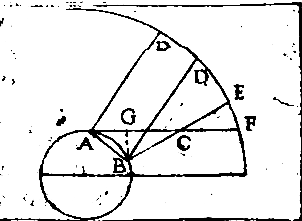
\includegraphics[max width=0.82\textwidth,max height=0.42\textheight,keepaspectratio]{images/figura01.png}\vspace{0.4em}\end{center}


Ed acciocchè V. S. Illustrissima vegga, ch'io non parlo così senza fondamento, ripigli la dimostrazion, ch'egli comincia alla fac. 123. del trattato della Cometa del 1577. ch'è nell'vltima parte de' suoi proginnasmi, nella quale volendo egli prouare, com'ella non fusse inferiore alla Luna per la conferenza dell'osseruazioni fatte da se in Vraniburg e da Tadeo Agapecio in Praga, prima tirata la subtesa A.B. all'arco dell'Orbe terrestre, che media trà i detti due luoghi e traguardando dal punto A. la stella fissa posta in D. suppone l'angolo D.A.B. esser retto, il che è molto lontano dal possibile, perche sendo la linea A.B. corda d'vn'arco minor di gr. 6. (come Ticcon medesimo afferma) bisogna, accioche il detto ang. sia retto, che la fissa D. sia lontana dal Zenit di A. meno di gr. 3. cosa ch'è tanto falsa, quanto che la sua minima distanza è più di gr. 48. essendo per detto dell'istesso Ticcone, la declinazion della fissa D. ch'è l'Aquila, ò vogliamo dire l'Auuoltoio di gr. 7.52. verso Borea, è la latitudine di Vraniburg gr. 55.54. In oltre egli scriue la medesima stella fissa da i due luoghi A. e B. vedersi nel medesimo luogo dell'ottaua sfera, perche la Terra tutta, non che la piccola parte A.B. non hà sensibil proporzione coll'immensità d'essa ottaua sfera. Ma perdonimi Ticcone, la grandezza, e piccolezza della Terra non hà che fare in questo caso, perche il vedersi da ogni sua parte la medesima stella nell'istesso luogo deriua dall'essere ella realmente nell'ottaua sfera, e non da altro; in quel modo à punto, che i caratteri, che sono sopra questo foglio, giamai rispetto al medesimo foglio non muteranno apparenza di sito per qualunque grandissima mutazion di luogo che faccia l'occhio di V. S. Illustriss. che gli riguarda, ma ben vno oggetto posto trà l'occhio, e la carta, al mouimento della testa varierà l'apparente sito, rispetto a' caratteri, sì che il medesimo carattere ora se gli vedrà dalla destra, ora dalla sinistra, ora più alto, ed ora più basso, \& in cotal guisa mutano apparente luogo i Pianeti nell'Orbe stellato, veduti da differenti parti della Terra, perche da quello sono lontanissimi. E quello che in questo caso opera la piccolezza della Terra, è che, faccendo i più lontani da noi minor varietà d'aspetto, ed i più vicini maggiore, finalmente per vno lontanissimo la grandezza della Terra non basti à far tal varietà sensibile. Quello poi che soggiunge accadere conforme alle leggi de gli archi, e delle corde, vegga V. S. Illustriss. quant'ei sia da tali leggi lontano, anzi pure da' primi elementi di Geometria. Egli dice, le due rette A.B; B.D. esser perpendicolari alla AB. il che è impossibile, perche la sola retta, che viene dal vertice, è perpendicolare sopra la tangente, e le sue parallele; e queste non vengono altramente dal vertice, nè l'AB. è tangente, ò ad essa parallela. In oltre, ei le domanda parallele, \& appresso dice, che le si vanno à congiungere nel centro, doue, oltre alla contradizzione dell'esser parallele, e concorrenti, vi e che prolungate passano lontanissime dal centro, e finalmente conchiude, che venendo dal centro alla circonferenza sopra i termini dell'AB. elle sono perpendicolari, il che è tanto impossibile, quanto che delle linee tirate dal centro à tutti i punti della corda AB. sola quella che cade nel punto di mezo gli è perpendicolare, e quelle che cascano ne gli estremi termini sono più di tutte l'altre inclinate, \& oblique, vegga dunque V. S. Illustrissima à quali, e quante essorbitanze aurebbe il Sarsi fatto prestar l'assenso dal suo maestro, quando vero fusse ciò, ch'in questo proposito hà scritto, cioè che quello abbia seguitate le ragioni, e modi di dimostrar di Ticcone nel ricercar il luogo della cometa. Vegga di più il medesimo Sarsi, quant'io meglio di lui, senza adoperar'Astrologia, nè Telescopio, abbia penetrato, (non dirò i sensi interni dell'animo suo, perche per ispiar questi io non hò nè occhi nè anco orecchi) ma i sensi della sua scrittura, i quali son pur tanto chiari, e manifesti, che bisogno non ci è de gli occhi lincei gentilmente introdotti dal Sarsi, credo, per ischerzare vn poco sopra la nostra Academia. E perche è V. S. Illustriss, ed altri Principi, e Signori grandi son meco à parte nello scherzo, io per la dottrina di sopra insegnatami dal Sarsi, non curando molto i suoi motti, me la passerò sotto l'ombra loro, e per meglio dire, illustrerò l'ombra mia col loro splendore. Ma tornando al proposito, vegga com'egli di nuouo vuol pure ch'io abbia reputato gran mancamento nel P. Gr. l'auer' egli aderito alla dottrina di Ticcone, e risentitamente domanda, chi ei doueua seguitare; forse Tolomeo, la cui dottrina dalle nuoue osseruazioni in Marte è scoperta per falsa? forse il Copernico, dal quale più presto si deue riuocar' ognuno, mercè dell'Ipotesi vltimamente dannata? Doue io noto più cose; e prima replico, ch'è falsissimo ch'io abbia mai biasimato il seguitar Ticcone, ancorche con ragione auessi potuto farlo, come pur finalmente dourà restar manifesto à i suoi aderenti per l'Antiticcone del Sig. Caualier Chiaramonte, si che quanto quì scriue il Sarsi è molto lontano dal proposito, e molto più fuor del caso s'introducono Tolomeo, e Copernico, de' quali non si troua, che scriuessero mai parola attenente à distanze, grandezze, mouimenti, e teoriche di comete, delle quali sole, e non d'altro si è trattato, e con altrettanta occasione vi si poteuano accoppiare Sofocle, e Bartolo, ò Liuio. Parmi oltre a ciò, di scorgere nel Sarsi ferma credenza, che nel filosofare sia necessario appoggiarsi all'opinioni di qualche celebre Autore, sì che la mente nostra, quando non si maritasse col discorso d'vn'altro, ne douesse in tutto rimanere sterile, ed infeconda; e forse stima, che la Filosofia sia vn libro, e vna fantasia d'vn vomo, come l'Iliade, e l'Orlando Furioso, libri ne' quali la meno importante cosa è, che quello che vi è scritto, sia vero. S. Sarsi la cosa non istà così. La Filosofia è scritta in questo grandissimo libro, che continuamente ci sta aperto innanzi à gli occhi (io dico l'vniuerso) ma non si può intendere se prima non s'impara a intender la lingua, e conoscer i caratteri, ne' quali è scritto. Egli è scritto in lingua matematica, e i caratteri son triangoli, cerchi, \& altre figure Geometriche, senza i quali mezi è impossibile a intenderne vmanamente parola; senza questi è vn'aggirarsi vanamente per vn'oscuro laberinto. Ma posto pur anco, come al Sarsi pare, che l'intelletto nostro debba farsi mancipio dell'intelletto d'vn'altr'vomo (lascio stare, ch'egli facendo così tutti, e sè stesso ancora, copiatori, loderà in sè quello, che hà biasimato nel Signor Mario) e che nelle contemplazioni de' moti celesti si debba aderire ad alcuno, io non veggo per qual ragione ei s'elegga Ticcone, anteponendolo a Tolomeo, e à Nicolò Copernico, de' quali due abbiamo i sistemi del Mondo interi, e con sommo artificio costrutti, e condotti al fine; cosa ch'io non veggo, che Ticcone abbia fatta, se già al Sarsi non basta l'auer negati gli altri due, e promessone vn altro, se ben poi non esseguito, nè meno dell'auer conuinto gli altri due di falsità, vorrei che alcuno lo riconoscesse da Ticcone: perche, quanto à quello di Tolomeo, nè Ticcone nè altri Astronomi nè il Copernico stesso poteuano apertamente conuincerlo, auuenga che la principal ragione presa da i mouimenti di Marte, e di Venere, aueua sempre il senso in contrario; al quale dimostrandosi il disco di Venere nelle due congiunzioni e separazioni dal Sole pochissimo differente in grandezza da sè stesso, e quel di Marte perigeo, à pena 3. ò 4. volte maggiore, che quando è Apogeo, giàmai non si sarebbe persuaso dimostrarsi veramente quello 40. e questo 60. volte maggiore nell'vno, che nell'altro stato, come bisognaua, che fusse quando le conuersioni loro fussero state intorno al Sole, secondo il sistema Copernicano; tuttauia ciò esser vero e manifesto al senso, hò dimostrato io, e fattolo con perfetto Telescopio toccar con mano a chiunque l'hà voluto vedere. Quanto poi all'Ipotesi Copernicana, quando per beneficio di noi Cattolici da più sourana sapienza non fussimo stati tolti d'errore, ed illuminata la nostra cecità, non credo, che tal grazia e beneficio si fusse potuto ottenere dalle ragioni, \& esperienze poste da Ticcone. Essendo dunque sicuramente falsi li due sistemi, e nullo quello di Ticcone, non dourebbe il Sarsi riprendermi, se con Seneca desidero la vera constituzion dell'vniuerso; e benche la domanda sia grande, e da mè molto bramata, non però trà ramarichi, e lagrime deploro, come scriue il Sarsi, la miseria, e calamità di questo secolo, nè pur si troua minimo vestigio di tali lamenti in tutta la scrittura del S. M. ma il Sarsi, bisognoso d'adombrare, e dar'appoggio à qualche suo pensiero, ch'ei disideraua di spiegare, lo và da sè stesso preparando, e somministrandosi quegli attacchi, che da altri non gli sono stati sposti. E quando pur'io deplorassi questo nostro infortunio, io non veggo quanto acconciamente possa dire il Sarsi, indarno essere sparse le mie querele, non auendo io poi modo, nè facoltà di tor via tal miseria, perche à me pare, che appunto per questo aurei causa di querelarmi, ed all'incontro le querimonie allora non ci aurebbon luogo, quando io potessi tor via l'infortunio.



\par\bigskip\noindent\phantomsection\addcontentsline{toc}{section}{§ 7}{\Large\color{rubric}\textbf{7.}}\enspace Ma legga ormai V. S. Illustrissima. \textit{Et quoniam hoc loco, atque hoc ad disputationem ingressu confutanda ea mihi sunt, quæ minoris ponderis videntur. Illud ab homine perhumano, qualem illum omnes norunt, expectassem profectò nunquam, vt vel ipso Catone seuerior, lepores quosdam, ac sales, appositè à nobis inter dicendum vsurpatos, fastidiosè adeo auersaretur, vt irrideret potius, ac diceret Naturam, pœticis non delectari. At ego, pròh, quantum ab hac opinione distabam: Naturam Poetriam ad hanc vsque diem existimaui. Illa certè vix vnquam pompa, fructusque vllos parit, quorum flores, veluti ludibunda, non præmittat. Galilæum verò quis vnquam adeò durum, existimasset, vt à seuerioribus negotijs, festiua aliqua eorum condimenta longè ableganda censeret? Hoc enim Stoici potius est, quam Academici. Attamen iure is quidem nos }\textit{arguat, si grauissimas quæstiones iocis, ac salibus eludere potius quam explicare tentaremus: at vero, rationum inter grauissimarum pondera lepida aliquandò, ac salsa iocari quis vetat? Vetat enimuerò Academicus. non paremus; \& si illi nostra hæc vrbanitas non sapit? Plures habemus non minus eruditos, quos delectat. Neque enim hic fuit sensus virorum, \& genere, \& doctrina clarissimorum, qui nostræ disputationi interfuere, quibus sapienter omninò factum visum est, vt Cometes, triste infaustumque vulgo portentum, placido aliquo verborum lenimento tractaretur, ac propè mitigaretur. }\textit{Sed hæc leuia sunt inquis. ita est, ac proinde leuiter diluenda.}


Da quanto qui è scritto in poche parole sbrigandomi, dico che nè il S. M. nè io, siamo così austeri, che gli scherzi, e le soauità poetiche ci abbiano à far nausea, di che ci sieno testimoni l'altre vaghezze interserite molto leggiadramente dal P. Gr. nella sua scrittura, delle quali il S. M. non hà pur mosso parola per tassarle; anzi con gran gusto si son letti i natali, la cuna, le abitazioni, i funerali della cometa, e l'essersi accesa per far lume all'abboccamento, e cena del Sole, e di Mercurio, nè pur ci ha dato fastidio che i lumi fussero accesi 20. giorni dopo cena, nè meno il sapere, che dou'è il Sole le candele son superflue, ed inutili, e ch'egli non cena, ma desina solamente, cioè mangia di giorno, e non di notte, la quale stagione gli è del tutto ignota; tutte queste cose senza veruno scrupolo si sono trapassate, perche, dette in cotal guisa, non ci anno lasciato nulla da desiderare nella verità del concetto sotto cotali scherzi contenuto, il quale per esser per sè noto e manifesto, non auea bisogno d'altra più profonda dubitazione. Ma che in vna questione massima, e difficilissima, qual è il volermi persuadere trouarsi realmente, e fuor di burle in natura vn particolare orbe celeste per le comete, mentre che Ticcone non si può suiluppar nell'esplicazion della difformità del moto apparente di essa cometa, la mente mia debba quietarsi, e restar appagata d'vn fioretto poetico, al quale non succede poi frutto veruno, questo è quello che il S. M. rifiuta; e con ragione, e con verità dice, che la Natura non si diletta di Poesie; proposizion verissima, benche il Sarsi mostri di non la credere, e finga di non conoscer ò la Natura, ò la Poesia, e di non sapere, che alla Poesia sono in maniera necessarie le fauole, e finzioni, che senza quelle non può essere; le quali bugie son poi tanto abborrite dalla Natura, che non meno impossibil cosa è il ritrouaruene pur'vna, che il trouar tenebre nella luce. Ma tempo è ormai, che vegniamo à cose di momento maggiore; però legga V. S. Illustriss. quel che segue.



\par\bigskip\noindent\phantomsection\addcontentsline{toc}{section}{§ 8}{\Large\color{rubric}\textbf{8.}}\enspace \textit{Venio nunc ad grauiora. }\textit{Tribus potissimum argumentis Cometæ locum indagandum censuit Magister meus. Primum quidem per Parallaxis obseruationes, deinde ex incessu eiusdem, ac motu, denique ex ijs, quæ Tubo optico, in illo obseruarentur. Conatur Galilæus singulis abrogare fidem, eaque suis momentis priuare. Cum enim ostendissemus Cometam, ex varijs diuersorum locorum obseruationibus, paruam admodum passum esse aspectus diuersitatem, ac propterea suprà Lunam statuendum; ait ille argumentum ex Parallaxi desumptum nihil habere ponderis, nisi prius statuatur, sint ne illa, quæ obseruantur, vera, vnoque loco consistentia, an verò in speciem apparentia, ac vaga. }\textit{Rectè is quidem, sed non erat his opus. Quid enim, si statutum iam id haberetur? Certè cum certamen nobis præsertim esset cum Peripateticis, quorum sententia quamplurimos etiam }\textit{nunc sectatores recenset; frustrà ex apparentium numero Cometas exclusissemus, cum nullius nostrum animum pulsaret hæc dubitatio. Sanè Galilæus ipse, dum aduersus Aristotelem disputat, non acriori, ac validiori vtitur argumento, quam ex Parallaxi desumpto. Cur igitur simili, atque eadem prorsus in caussa, nobis eodem vti liberè non liceret?}


Per conoscer quanto sia il momento delle cose quì scritte, basterà restringere in breuità quello che dice il S. M. e questo, che gli viene opposto. Scrisse il S. M. in generale. Quelli che per via della Paralasse voglion determinar circa 'l luogo della Cometa, anno bisogno di stabilir prima, lei esser cosa fissa e reale, e non vn'apparenza vaga, atteso che la ragion della Paralasse conchiude ben negli oggetti reali, ma non negli apparenti, com'egli essemplifica in molti particolari. Aggiunge poi la mancanza di Paralasse rendere incompatibili le due proposizioni d'Aristotile, che sono, che la cometa sia vn incendio, ch'è cosa tanto reale, e sia in aria molto vicina alla Terra. Qui si leua sù il Sarsi, e dice. Tutto stà bene, ma è fuor del caso nostro, perche noi disputiamo contro Aristotile, e vana sarebbe stata la fatica in prouar, che la cometa non fusse vna apparenza; poiche noi conuegniamo con lui in tenerla cosa reale, e come di cosa reale il nostro argomento preso dalla Paralasse conchiude. Anzi (soggiunge egli) l'auuersario stesso non si serue d'argomento più valido contro Aristotile, e se ei se ne serue, perche nell'istessa causa non ce ne possiamo liberamente seruir noi ancora? Hor quì io non so quel, che il Sarsi pretenda, nè in qual cosa ei pensa d'impugnare il S. M. poiche ambedue dicono le medesime cose, cioè che la ragione della Paralasse non vale nelle pure apparenze, ma val ben ne gli oggetti reali, ed in conseguenza val contro Aristotile, mentr'ei vuole, che la Cometa sia cosa reale. Quì se si debbe dire il vero con pace del Sarsi, non si può dir altro, se non ch'egli co'l palliare il detto del S. Mario hà voluto abbarbagliar la vista al lettore, si che gli resti concetto che il S. Mario abbia parlato à sproposito, perche à voler che l'obbiezzioni del Sarsi auessero vigore, bisognerebbe, che doue il S. Mario parlando in generale a tutto il Mondo dice. A chi vuol, che l'argomento della Paralasse militi nella cometa, conuien, che proui prima, quella esser cosa reale, bisognerebbe dico, che auesse detto. Se il P. Gr. vuole che l'argomento della Paralasse militi contro Aristotile, che tiene la cometa esser cosa reale, e non apparente, bisogna che prima proui, che la cometa sia cosa reale, e non apparente, e così il detto del S. Mario sarebbe veramente, quale il Sarsi lo vorrebbe far apparire, vn grandissimo sproposito, ma il S. M. non hà mai, nè scritte, nè pensate queste sciocchezze.



\par\bigskip\noindent\phantomsection\addcontentsline{toc}{section}{§ 9}{\Large\color{rubric}\textbf{9.}}\enspace \textit{Sed confutandæ etiam fuerint Anaxagoræ, Pythagoræorum atque Hippocratis opiniones. Nemo tamen ex ijs cometam vanum omni ex parte oculorum ludibrium affirmarat. Anaxagoras enim Stellarum verissimarum congeriem esse dixit; cum Aeschylo Hippocrates nihil à Pythagoræis dissentit: Aristoteles profectò cum eorundem Pythagoræorum sententiam exposuisset, quia dicerent Cometam vnum esse errantium siderum, tardissimè ad nos accedens, ac citissimè fugiens, subdit. Similiter autem his, \& qui sub Hippocrate Chio, \& discipulo eius Aeschylo, enunciauerunt. Sed comam non ex se ipso aiunt habere: sed errantem, propter locum aliquando accipere refracto nostro visu ab humore attracto ab ipso ad Solem. Galilæus verò in ipso suæ disputationis exordio, dum eorumdem placita }\textit{recenset: asserit dixisse illos Cometam stellam quandam fuisse, quæ Terris aliquandò propior facta, quosdam ab eadem ad se vapores extraheret, e quibus sibi non caput, sed comam decenter aptaret. Minus igitur, vt hoc obiter dicam, ad rem facit; dum postea ex his ijsdem locis probat, Pythagoræos etiam existimasse Cometam ex refractione luminis extitisse. illi enim nihil in Cometis vanum, præter barbam, existimarunt. Intelligit ergo nulli horum visum vnquam fuisse, Cometam, si de eiusdem capite loquamur, inane quiddam, ac merè apparens dicendum. Quare cum hac in re, ad hoc vsque tempus, conuenirent omnes, quid erat causæ, cur facem hanc lucidissimam laruis illis, ac fictis colorum ludibrijs spoliaremus, ab eaque crimen illud auerteremus, quod ei nullus hominum, quorum habenda foret ratio, obiecisset? Cardanus enim ac Telesius, ex quibus aliquid ad hanc rem desumpsisse videtur Galilæus, sterilem, atque infelicem Philosophiam nacti; nulla ab ea prole beati, libros posteris, non liberos reliquerunt. Nobis igitur, ac Tychoni satis sit apud eos non perperam disputasse, apud quos nunquam vani, ac fallacis spectri Cometes incurrit suspicionem; hoc est ipso Galilæo teste, apud omnium, quot quot adhuc fuerunt, Philosophorum Academias. Quod si quis modo inuentus est, qui hæc phænomena inter merè apparentia reponenda disertè docuerit; ostendam huic ego suo loco, ni fallor, quam longè Cometæ ab Iride, Areis, \& Coronis, moribus, ac motibus distent, quibusque argumentis conficiatur, Cometem, si comam excluseris, non ad Solis imperium, nutumque, quod apparentibus omnibus commune est, agi; sed liberum moueri protinus ac circumferri, quò sua illum Natura impulerit, traxeritque.}


Quì volendo anco in vniuersale mostrar la dubitazion promossa dal S. M. esser vana, e superflua, dice, niuno Autore antico, ò moderno degno d'esser'auuto in considerazione, auer mai stimato la cometa potere esser vna semplice apparenza, e che per ciò al suo Maestro, il quale solo con questi disputaua, e di questi soli aspiraua alla vittoria, niun mestier faceua di rimuouerla dal numero de' puri simulacri. Al che io rispondendo dico primieramente, che il Sarsi ancora con simil ragione poteua lasciare stare il S. Mario, e mè, poi che siam fuori del numero di quegli antichi, e moderni, contro i quali il suo Maestro disputaua, ed abbiamo auuta intenzione di parlar solamente con quelli (sieno antichi, ò moderni) che cercano con ogni studio d'inuestigar qualche verità in Natura, lasciando in tutto e per tutto ne' lor panni quegli, che solo per ostentazione in strepitose contese aspirano ad esser con pomposo applauso popolare giudicati, non ritrouatori di cose vere, ma solamente superiori à gli altri; nè doueua mettersi con tanta ansietà per atterrar cosa, che nè à se, nè al suo Maestro era di pregiudicio. Doueua secondariamente considerare, che molto più è scusabile vno, à chi in alcuna professione non cade in mente qualche particolare attenente à quella, e massime quando, nè anco à mille altri, che abbiano professato il medesimo, è souuenuto, che quegli, à cui venga in mente, e presti l'assenso à cosa, che sia vana, ed inutile in quell'affare, ond'ei poteua, e doueua più tosto confessare, che al suo Maestro, com'anco a nessun de' suoi antecessori, non era passato per la mente il concetto, che la cometa potesse essere vna apparenza, che sforzarsi, per dichiarar vana la considerazion souuenuta à noi, perche quello, oltre che passaua senza niuna offesa del suo Maestro, daua indizio, d'vna ingenua libertà, e questo, non potendo seguire senza offesa della mia reputazione (quando gli fusse sortito l'intento), dà più tosto segno d'animo alterato da qualche passione. Il S. Mario con isperanza di far cosa grata, e profitteuole àgli studiosi del vero propose con ogni modestia, che per l'auuenire fusse bene considerare l'essenza della cometa, e s'ella potesse esser cosa non reale, ma solo apparente, e non biasimò il P. Gr. nè altri, che per l'addietro non l'auesser fatto. Il Sarsi si leua sù, e con mente alterata cerca di prouare, la dubitazione essere stata fuor di proposito, ed esser di più manifestamente falsa; tuttauia per trouarsi, come si dice, \textit{in vtrumque paratus}, in ogni euento, ch'ella apparisse pur degna di qualche considerazione, per ispogliarmi di quella lode che arrecar mi potesse, la predica per cosa vecchia del Cardano, e del Telesio, ma disprezzata dal suo Maestro, come fantasia di Filosofi deboli, e di niun seguito, ed in tanto dissimola, e non sente con quanta poca pietà egli spoglia, e denuda coloro di tutta la reputazione, per ricoprire vn piccolissimo neo di quella del suo Maestro. Se voi Sarsi vi fate scolare di quei Venerandi Padri nella natural Filosofia, non vi fate già nella morale, perche non vi sarà creduto. Quello che abbiano scritto il Cardano e 'l Telesio, io non l'hò veduto, ma per altri riscontri, che vedremo appresso, posso facilmente conghietturare che il Sarsi non abbia ben penetrato il senso loro. In tanto non posso mancare, per auuertimento suo e per difesa di quelli, di mostrar quanto improbabilmente ei conclude la lor poca scienza della Filosofia dal piccol numero de' suoi seguaci. Forse crede il Sarsi, che de' buoni Filosofi se ne trouino le squadre intere dentro ogni ricinto di mura? Io S. Sarsi credo, che volino, come l'Aquile, e non come gli storni. E ben vero, che quelle perche son rare, poco si veggono, e meno si sentono, e questi, che volano à stormi, douunque si posano, empiendo il Ciel di strida, e di rumori, metton sozzopra il mondo. Ma pur fussero i veri Filosofi, come l'Aquile, e non più tosto come la Fenice. S. Sarsi. Infinita è la turba de gli sciocchi, cioè di quelli, che non sanno nulla; assai son quelli, che sanno pochissimo di Filosofia; pochi son quelli che ne sanno qualche piccola cosetta; pochissimi quelli che ne sanno qualche particella; vn solo Dio è quello che la sà tutta. Sì che per dir quel, ch'io voglio inferire, trattando della scienza, che per via di dimostrazione, e di discorso vmano si può da gli vuomini conseguire, io tengo per fermo, che quanto più essa participerà di perfezzione, tanto minor numero di conclusioni prometterà d'insegnare, tanto minor numero ne dimostrerà, ed in conseguenza tanto meno alletterà, e tanto minore sarà il numero de' suoi seguaci. Ma per l'opposito, la magnificenza de' titoli, la grandezza, e numerosità delle promesse, attrændo la natural curiosità de gli vuomini, e tenendogli perpetuamente rauuolti in fallacie, e chimere, senza mai far loro gustar l'acutezza d'vna sola dimostrazione, onde il gusto risuegliato abbia à conoscer l'insipidezza de' suoi cibi consueti, ne terrà numero infinito occupato, e gran ventura sarà d'alcuno, che, scorto da straordinario lume naturale, si saprà torre da i tenebrosi, e confusi laberinti, ne i quali si sarebbe coll'vniuersale andato sempre aggirando e tuttauia più auuiluppando. Il giudicar dunque dell'opinioni d'alcuno in materia di Filosofia dal numero de i seguaci, lo tengo poco sicuro. Ma ben ch'io stimi piccolissimo poter esser il numero de i seguaci della miglior Filosofia, non però concludo, pel conuerso, quelle opinioni e dottrine esser necessariamente perfette, le quali anno pochi seguaci, imperocchè io intendo molto bene, potersi da alcuno tenere opinioni tanto erronee, che da tutti gli altri restino abbandonate. Ora, da qual de' due fonti deriui la scarsità de' seguaci de' due Autori nominati dal Sarsi per infecondi e derelitti, io non lo sò, nè hò fatto studio tale nell'opere loro, che mi potesse bastar per giudicarle. Ma tornando alla materia, dico, che troppo tardi mi par, che il Sarsi voglia persuaderci, che il suo Maestro, non perche non gli cadesse in mente, ma perche disprezzò, come cosa vanissima, il concetto che la cometa potess'essere vn puro simulacro, e che in questi non milita l'argomento della Paralasse, non ne fece menzione, tarda, dico, è cotale scusa, perche quand'egli scrisse nel suo Problema: \textit{Statuo, rem quamcunque inter firmamentum \& terram constitutam, si diuersis è locis spectetur, diuersis etiam firmamenti partibus responsuram}. Chiaramente si dimostrò non gli esser venuto in mente l'Iride e l'Alone, i Parelij ed altre riflessioni, che à tal legge non soggiacciono, le quali ei doueua nominare, \& eccettuare, e massime, ch'egli stesso, lasciando Aristotile, inclina all'opinione del Kepplero, che la cometa possa essere vna riflessione. Ma seguendo più auanti, mi par di vedere che il Sarsi faccia gran differenza dal capo della cometa alla sua barba, ò chioma, e che quanto alla chioma possa esser veramente ch'ella sia vn'illusione della nostra vista, e vna apparenza, e che tale l'abbiano stimata ancora quei Pittagorici nominati da Aristotile; ma quanto al capo stima, che sia necessariamente cosa reale, e che niuno l'abbia mai creduto altrimenti. Or quì vorrei io vna bene specificata distinzione trà quello, che il Sarsi intende per reale, e quello, ch'egli stima apparente, e qual cosa sia quella che fà esser reale quello, ch'è reale, e apparente quello, ch'è apparente. Perche s'egli chiama il capo reale, per esser in vna sostanza, e materia reale, io dico che anco la chioma è tale; sì che chi leuasse via quei vapori ne' quali si fà la reflession della vista nostra al Sole, sarebo tolta parimente la chioma, come al tor via delle nuuole, si toglie l'Iride e l'Alone, e s'ei domanda la chioma finta, perche senza la riflession della vista al Sole ella non sarebbe, io dico che anco del capo seguirebbe l'istesso, si che tanto la chioma, quanto il capo non son'altro, che reflession di raggi in vna materia qualunqu'ella si sia; e che in quanto riflessioni sono pure apparenze, in quanto alla materia son cosa reale; e se il Sarsi ammette, che alla mutazion di luogo del riguardante faccia, ò possa far mutazion di luogo, la generazion della chioma nella materia, io dico, che del capo ancora può nel medesimo modo seguir l'istesso, e non credo, che quei Filosofi antichi stimassero altrimenti, perche, se v. g. auesser creduto il capo esser realmente vna stella per sè stessa, lucida, e consistente, e solo la chioma apparente, aurebber detto, che quando per l'obliquità della sfera non si fà la refrazzion della nostra vista al Sole, non si vede più la chioma, ma si ben la stella, ch'è capo della cometa; il che non dissero, ma dissero che in tutto non si vedeua cometa; segno euidente la generazion d'ambedue esser l'istessa. Ma detto, ò non detto, che ciò sia da gli antichi, vien messo in considerazione adesso dal S. Mar. con assai sensate ragioni di dubitare, le quali deuono esser ponderate, come pure fà ancora l'istesso Sarsi; e noi à suo luogo anderemo considerando quanto egli ne scriue.



\par\bigskip\noindent\phantomsection\addcontentsline{toc}{section}{§ 10}{\Large\color{rubric}\textbf{10.}}\enspace Intanto segua V. S. Illustriss. di leggere. \textit{Eadem prorsus ratione respondendum mihi est ad ea, quæ argumento ex motu desumpto obijciuntur. Nos enim ex eo, quòd loca Cometæ singulis diebus respondentia in plano ad modum horologij descripta, in vna recta linea reperirentur; }\textit{motum illum in circulo maximo fuisse necessariò inferebamus. Obijcit autem Galilæus non deduci id necessariò; quia si incessus Cometæ reuera in linea recta fuisset, sic etiam loca ipsius, ad modum horologij descripta lineam rectam constituissent; non tamen fuisset motus hic in circulo maximo. Sed quamuis verissimum sit, motum etiam per lineam rectam repræsentari debuisse rectum: cum tamen aduersus eos lis esset, qui vel de Cometæ motu circulari nihil ambigerent, vel quibus rectus hic motus nunquam venisset in mentem: hoc est contra Anaxagoram, Pythagoræos, Hippocratem, \& Aristotelem; atque illud tantum quæreretur, an Cometes, qui in orbem agi credebatur, maiores, an potius minores, lustraret orbes; non ineptè, sed prorsus necessariò, ex motu in linea recta apparente inferebatur circulus eo motu descriptus maximus fuisse. Nemo enim adhuc motum hunc rectum, \& perpendicularem inuexerat. Quamuis enim }\textit{Keplerus ante Galilæum, in appendicula de motu Cometarum, per lineas rectas eundem motum explicare contendat: ille tamen nihilominus vidit, in quales sese difficultates indueret; Quare neque ad Terram perpendicularem esse voluit motum hunc; sed transuersum, neque æqualem, sed in principio ac fine remissiorem, celerium in medio, eumque præterea fulciendum terræ ipsius motu circulari existimauit, vt omnia Cometarum Phœnomena explicaret. Quæ nobis Catholicis nulla ratione permittuntur. Ego igitur opinionem illam, quam piè, ac sanctè tueri non liceret, pro nulla habendam duxeram. Quòd si postea paucis mutatis, motum hunc rectum Cometis tribuendum putauit Galilæus; id quam non rectè præstiterit inferius singillatim mihi ostendendum erit. Intelligat interim, nihil nos contra Logicæ præcepta }\textit{peccasse, dum ex motu in linea recta apparente orbis maximi partem eodem descriptam fuisse deduximus. Quid enim opus fuerat motum illum rectum \& perpendicularem excludere,}\textit{ }\textit{quem in Cometis nusquam reperiri constabat.}


Aueua il Sig. Guiducci, con quell'onestissimo fine d'ageuolar la strada agli studiosi del vero, messo in considerazione l'equiuoco, che prendeuano quegli che, dall'apparir la cometa mossa per linea retta, argumentauano il mouimento suo esser per cerchio massimo, auuertendogli, che, se bene era vero, che il moto per cerchio massimo sempre appariua retto, non era però necessariamente vero il conuerso, cioè che il moto, che apparisse retto fusse per cerchio massimo, come veniuano ad auer supposto quegli, che dall'apparente moto retto inferiuano, la cometa muouersi per cerchio massimo: trà i quali era stato il P. Gr. il quale forse quietandosi nell'autorità di Ticcone, che prima aueua equiuocato, trapassò quello, che forse non aurebbe passato quando non auesse auuto tal precursore; il che rende assai scusabile appresso di mè il piccolo errore del Padre, il quale credo anco, che dell'auuertimento del S. M. abbia fatto capitale, e tenutogliene buon grado. Vien'ora il Sarsi, e continuando nel suo già impresso affetto, s'ingegna di far apparir l'auuertimento innauuertenza e poca considerazione, credendo in cotal guisa saluar' il suo Maestro, ma à me pare che ne segua contrario effetto (quando però il Padre prestasse il suo assenso alle scuse, e difese del Sarsi), e che per ischiuare vn'error solo incorrerebbe in molti. E prima seguitando il Sarsi di reputar vano, e superfluo l'auuertir quelle cose, che nè esso, nè altri hà auuertite, dice, che disputando il suo Maestro con Ar. e con Pittagorici, che mai non aueuano introdotto per le comete mouimento retto, fuor del caso sarebbe stato, ch'auesse tentato di rimuouerla. Ma se noi ben considereremo, questa scusa, non solleua punto il P. perche non auendo mai li medesimi auuersari introdotto per le comete il moto per cerchi minori, altrettanto resta superfluo il dimostrar, ch'elle si muouano per cerchi massimi. Bisogna dunque al Sarsi, ò trouar, che quegli antichi abbiano scritto, le comete muouersi per cerchi minori, ò confessare che il suo Maestro sia del pari stato superfluo nel considerare il moto per cerchio massimo, come sarebbe stato nel considerare il retto. Anzi (e sia per la seconda instanza), stando pur nella regola del Sarsi, assai maggior mancamento è stato il lasciar senza considerazione il moto retto, poi che pur v'era il Kepplero, che attribuito l'aueua alle comete, ed il medesimo Sarsi lo nomina. Nè mi pare che la scusa, ch'egli adduce sia del tutto sofficiente, cioè che per tirarsi tale opinion del Kepplero in conseguenza la mobilità della Terra, proposizione, la quale piamente e santamente non si può tenere, egli per ciò la reputaua per niente. Perche questo doueua più tosto essergli stimolo à distruggerla, e manifestarla per impossibile, e forse non è mal fatto il dimostrar' anco con ragioni naturali, quando ciò si possa, la falsità di quelle proposizioni, che son dichiarate repugnanti alle scritture sacre. Terzo resta ancor mancheuole la scusa del Sarsi, perche non solamente il moto veramente retto apparisce per linea retta, ma qualunque altro, tuttauolta, che sia fatto nel medesimo piano, nel quale è l'occhio del riguardante, il che fu pure accennato dal S. M. si che bisognerà al Sarsi trouar modo di persuaderci, che nè anco alcuno altro mouimento fuor del circolare sia mai caduto in mente ad alcuno potersi assegnare alle comete, il che non sò quanto acconciamente gli potesse succedere, perche quando niuno altro l'auesse detto, l'ha pure egli stesso scritto pochi versi di sotto, quando, per difesa della digression dal Sole di più di 90 gradi, ei dà luogo al moto non circolare, \& ammette quello per linea ouata, anzi pur bisognando per qualsiuoglia linea irregolare ancora. E dunque necessario, ò che l'istesso mouimento sia or circolare, or'ouale, or del tutto irregolare, secondo il bisogno del Sarsi, ò ch'ei confessi la difesa pel suo Maestro esser difettuosa. Quarto, ma che sarà quando io ammetta, il moto della cometa esser, non solo per commune opinione, ma veramente, e necessariamente, circolare? stimerà forse il Sarsi, esser perciò dal suo Maestro, ò da altri dall'apparir quello per retta linea, concludentemente dimostrato esser per cerchio massimo? Sò che il Sarsi hà sin'ora creduto di sì, e si è ingannato, ed io lo trarrei d'errore, quando credessi di non gli dispiacere; e per ciò fare l'interrogherei, quali nella sfera ei domanda cerchi massimi. Sò che mi risponderebbe, quelli che passando per lo centro di quella (ch'è anco il centro della Terra), la diuidono in due parti vguali. Io gli soggiungerei. Adunque i cerchi descritti da Venere, da Mercurio e da' Pianeti Medicei non sono altrimenti cerchi massimi, anzi piccolissimi, auendo questi per lor centro Gioue, e quelli il Sole; tuttauia se s'osseruerà quali si mostrino i mouimenti loro, gli troueremo apparir per linee rette; il che auuiene per esser l'occhio nostro nel medesimo piano nel quale son anco i cerchi descritti dalle nominate stelle. Concludiamo per tanto che dall'apparirci vn moto retto, altro non si può concludere, saluo, che l'esser fatto, non per la circonferenza d'vn cerchio massimo, più che per quella d'vn minore, ma solamente esser fatto nel piano, che passa per l'occhio, cioè nel piano d'vn cerchio massimo; e che in sè stesso quel moto può esser fatto per linea circolare, ed anco per qualsiuoglia altra, quantosiuoglia irregolare, chè sempre apparirà retto, e che però, non essendo le due proposizioni già da noi essaminate conuertibili, il prender l'vna per l'altra è vn equiuocare, ch'è poi peccare in Logica. Se io credessi che il Sarsi non fusse per volermene male, vorrei che noi gli conferissimo vn'altra simil fallacia, la quale veggo, ch'è da grandissimi vuomini trapassata, e forse l'istesso Sarsi non vi hà fatto riflessione; ma non vorrei fargli dispiacere col mostrargli di non l'auer io ancora con tanti altri più perspicaci di mè trascorsa, ma sia come si voglia, la voglio conferire à V. S. Illustriss. E stato con arguta osseruazion notato, che l'estremità della coda, il capo delle comete ed il centro del disco del Sole si scorgono sempre secondo la medesima linea retta: dal che si è preso gagliarda conghiettura detta coda essere vna distesa refrazzione del lume solare diametralmente opposta al Sole; ned'è, per quanto io sappia, sin quì caduto in considerazione ad alcuno, come il mostrarcisi il Sole, e tutto il tratto della cometa in linea retta non conchiuda, che necessariamente la linea retta tirata per l'estremità della coda, e pel capo della cometa vada prolungata à terminar nel Sole. Per apparir trè, ò più termini in linea retta, basta che sieno collocati nel medesimo piano, che l'occhio. E così, per essempio, Marte, ò la Luna talora si vederanno in mezo direttamente trà due stelle fisse, ma non perciò la linea retta che congiungesse le due stelle passerebbe per Marte, ò per la Luna. Dall'apparir dunque la coda della cometa direttamente opposta al Sole, altro non si può necessariamente conchiudere, che l'esser nel medesimo piano coll'occhio. Or sia, nel quinto luogo notata certa, dirò così, circostanza nelle parole verso il fine delle lette da V. S. Illustriss. e da mè essaminate, doue il Sarsi si prende assunto di voler più a basso mostrare, quanto malamente io, cioè il S. M. abbia attribuito alla cometa il moto retto, e poi trè versi più a basso, dice non esser bisogno alcuno d'escluder questo moto retto, il qual'era certo, e manifesto già mai non ritrouarsi nelle comete; ma se l'impossibilità di questo moto è certa, e manifesta, à che proposito mettersi à volerla escludere? ed in qual modo è ella certa, e manifesta, se per detto del Sarsi, nessuno l'hà pur mai non solamente confutata, ma nè anco considerata? Al Kepplero solo, dic'egli è tal moto venuto in considerazione, ma il Kepplero non lo confuta, anzi l'introduce per possibile, e vero. Parmi che 'l Sarsi sentendosi di non poter far' altro, cerchi d'auuiluppare il Lettore, ma io cercherò di disfare i viluppi.



\par\bigskip\noindent\phantomsection\addcontentsline{toc}{section}{§ 11}{\Large\color{rubric}\textbf{11.}}\enspace \textit{Sed dum illud præterea hoc loco nobis obijcit: Si Cometes circa Solem ageretur, cum integro quadrante ab eodem Sole recesserit, futurum aliquandò, vt ad Terram vsque descenderet; non venit illi in mentem fortassè, non vno modo circa Solem cometam agi potuisse. Quid enim, si circulus, quo vehebatur eccentricus Soli fuisset? \& maiori sui parte, aut supra Solem existente, aut ad Septentrionem vergente? }\textit{Quid si motus circularis non fuisset, sed Ellipticus, \& quidem summa, imaque parte compressus, longe vero exporrectus in latera? Quid si ne Ellipticus quidem, sed omnino irregularis; cum, præsertim, ex ipsius Galilæi Systemate, nullo planè impedimento Cometis quocunque liberet moueri licuerit? }\textit{Vt sanè propterea timendum non esset, ne Cometarum lucem Tellus, aut Tartarus è propinquo visurus vmquam foret.}


Quì primieramente se io ammetto l'accusa che mi dà il Sarsi di poco considerato, mentre non mi siano venuti in mente i diuersi moti ch'attribuir si possono alla cometa, non sò com'egli potrà scolpare dalla medesima nota il suo Maestro, il quale non considerò il potersi ella muouer di moto retto; e s'egli scusa il suo Maestro col dire che tal considerazione sarebbe stata superflua, non sendo stato da niun altro Autore introdotto tal mouimento, non veggo di meritar d'essere accusato io, ma sì ben nell'istesso modo debbo essere scusato, non si trouando Autor nessuno, ch'abbia introdotti questi moti stranieri, ch'ora nomina il Sarsi. In oltre, S. Sarsi toccaua al vostro Maestro, e non à mè, à pensare à questi mouimenti, per li quali si potesse render conueneuol ragione delle digressioni così grandi della cometa, e se alcuno ve n'è accommodato a tal bisogno, doueua nominarlo, e quel solo accettare, e non lasciarlo sotto silentio, e introdurre con Ticcone il semplice circolare intorno al Sole, inettissimo à saluar cotale apparenza, e voler poi, che non esso, ma noi auessimo commesso fallo in non indouinare, ch'ei potesse internamente auer dato ricetto à pensieri diuersissimi da quello, ch'aueua scritto. Di più, il S. M. non hà mai detto. che non sia in Natura modo alcuno di saluar la digressione d'vna quarta (anzi se tal digressione è stata, ben chiara cosa è, che ci è anco il modo com'ella è stata); ma hà detto nell'Ippotesi riceuuta dal P. non si può far tal digressione senza, che la cometa tocchi la Terra, e anco la penetri. Vana dunque è sin qui la scusa del Sarsi. Ma fors'ei pretende, ch'ogni leggiera scusa si debba ammettere per lo suo Maestro, ma che per mè ogni più gagliarda resti inualida, e se questo è, io volentieri mi quieto, e liberamente gliel concedo. E vengo, nel secondo luogo à produrre altra scusa per mè (vestito della persona del S. M.); e con ingenuità confessando non m'esser venuti in mente i mouimenti per eccentrici, ò per linee ouali, ò per altre irregolari, dico ciò essere accaduto perch'io non soglio dar'orecchio a' concetti, che non anno, che fare in quel proposito di che si tratta. E che vuol fare il Sarsi del moto intorno al Sole in vna figura ouale, per far digredir la cometa vna quarta? cred'egli forse, che coll'allungar per vn verso e stringer per l'altro tal figura, gli possa succedere l'intento? certo nò, quando anco ei l'allungasse in infinito. E la medesima impossibilità cade nell'eccentrico, che sia per la minor parte sotto il Sole.


\begin{center}\vspace{0.4em}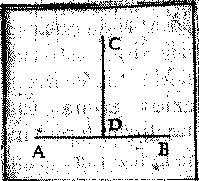
\includegraphics[max width=0.82\textwidth,max height=0.42\textheight,keepaspectratio]{images/figura02.png}\vspace{0.4em}\end{center}


E per intelligenza del Sarsi, V. S. Illustriss. potrà vna volta incontrandolo, proporgli due tali linee rette AB. CD. delle quali la CD. sia perpendicolare all'AB. e dirgli, che supponendo la retta DC. esser quella, che và dall'occhio al Sole, quella per la quale si hà da vedere la cometa digredita 90. gr. bisogna che di necessità sia la BA. o vero DB. essendo communemente conceduto, il moto apparente della cometa esser nel piano d'vn cerchio massimo. Lo preghi poi, che per nostro ammæstramento egli descriua l'eccentrico, ò l'ouato nominati da lui, per li quali mouendosi la cometa possa abbassarsi tanto ch'ella venga veduta per la linea ADB. perche io confesso di non lo saper fare, e sin quì vengono esclusi due de' proposti modi; ci resta l'altro eccentrico col centro dechinante à destra, ò a sinistra della linea DC. e la linea irregolare. Quanto all'eccentrico è vero, che non è del tutto impossibile à disegnarsi in carta, in maniera, che causi la cercata digressione; ma dico bene al Sarsi che s'ei si metterà à delinear' il Sole cogli Orbi di Mercurio, e di Venere attorno, e di più la Terra circondata dall'Orbe della Luna, come di necessità conuien fare l'vno, e l'altro, e poi si porrà a volerui ingarbare vn tale eccentrico per la cometa, credo certo, che se gli rappresenteranno tali essorbitanze, e mostruosità, che quando bene con tale scusa ei potesse solleuare il suo Maestro, si spauenterebbe a farlo. Quanto poi alle linee irregolari, non è dubbio nessuno, che non solamente questa, ma qualsiuoglia altra apparenza si può saluare. Ma voglio auuertire il Sarsi, che l'introdur tal linea non pur non giouerebbe alla causa del suo Maestro, ma più grauemente gli pregiudicherebbe, e questo non solamente perch'ei non l'ha nominata mai, anzi accettò la linea circolare regolarissima, per così dire, sopra ogn'altra, ma perche maggior leggerezza sarebbe stata il proporla, il che potrebbe intendere il Sarsi medesimo, tuttauolta ch'ei considerasse che cosa importi linea irregolare. Chiamansi linee regolari quelle, che auendo la lor descrizzione vna, ferma, e determinata, si possono definire, e di loro dimostrare gli accidenti, e proprietà: e così la spirale, e regolare, e si definisce nascer da due moti vniformi, l'vn retto, e l'altro circolare, così l'ellittica, nascendo dalla sezzion del cono, e del cilindro, \&c. Ma le linee irregolari son quelle, che, non auendo determinazion veruna, sono infinite, e casuali, e perciò indefinibili, nè di esse si può, in conseguenza dimostrar proprietà alcuna, nè in somma saperne nulla; si che il voler dire, il tale accidente accade, mercè di vna linea irregolare, è il medesimo, che dire, io non so perche ei s'accaggia, e l'introduzzione di tal linea non è punto migliore delle simpatie, antipatie, proprietà occulte, influenze ed altri termini vsati da alcuni Filosofi per maschera della vera risposta, che sarebbe. Io non lo sò. Risposta tanto più tollerabile dell'altra, quant'vna candida sincerità è più bella d'vn'inganneuol doppiezza. Fù dunque molto più auueduto il P. Gr. à non propor cotali linee irregolari come bastanti à soddisfare al quesito, che il suo scolare à nominarle. E ben vero, s'io deuo liberamente dire il mio parere, che io credo, che il Sarsi medesimo abbia benissimo ed internamente compresa l'inefficacia delle sue risposte, e che poco fondamento ci abbia fatto; sopra il che conghietturo io dall'essersene con gran breuità spedito, ancorche il punto fusse principalissimo nella materia, che si tratta, e le difficoltà promosse dal S. M. grauissime: ed egli di sè medesimo mi è buon testimonio mentre, alla fac. 16. parlando di certo argomento vsato dal suo Maestro, scriue: \textit{Cæterùm quanti hoc argumentum apud nos esset, satis arbitror, ex eo poterat intelligi, quod paucis adeò, ac planè ieiunè propositum fuerit, cùm prius reliqua duo longè accuratiùs ac fusiùs fuissent explicata}. E con qual breuità, e quanto sobbriamente egli abbia tocco questo, veggasi, oltre all'altre cose, dal non auer pur fatte le figure degli eccentrici e dell'ellissi, introddotte per saluare il tutto; doue che più à basso incontreremo vn mar di disegni inseriti in vn lungo discorso per riprouar poi vna esperienza che in vltimo non reca pure vn minimo ristoro alla principale intenzione che si hà in quel luogo. Ma, senz'andar più lontano, entri pur V. S. Illustrissima in vn'Oceano di distinzioni, sillogismi \& altri termini logicali, e trouerà esser fatta dal Sarsi stima grandissima di cosa, che liberamente parlando, io stimo assai meno della lana caprina.



\par\bigskip\noindent\phantomsection\addcontentsline{toc}{section}{§ 12}{\Large\color{rubric}\textbf{12.}}\enspace \textit{Sed quando Magistro meo Logicæ imperitiam Galilæus obiecit, patiatur experiri nos, quàm exactè eiusdem ipse facultatis leges seruauerit: neque hoc multis; vno enim aut altero exemplo contenti erimus. Dixeramus Stellas Tubo inspectas minimum, ad sensum; incrementum suscepisse. Sed cum Stellæ, inquit ille, quamplurimæ, quæ perspicacissimos quosque oculos fugiunt, per Tubum conspiciantur; non insensibile, sed infinitum potius, incrementum ab illo accepisse dicendæ erunt. nihil enim, atque aliquid, infinito planè distant interuallo. Ex eo igitur; quòd aliquid videatur, cum prius non videretur, infert Galilæus obiecti incrementum infinitum, incrementum inquam, apparens saltem, quantitatis. At ego, neque infinitum, neque incre}\textit{mentum quidem vllum inferri posse existimo. Et primo quidem, quamquam verum sit inter hoc quod est videri, \& hoc quod est non videri, distantiam esse infinitam vna saltem ex parte, atque hæc duo proportionem illam habere, quam Nihil, atque Aliquid, hoc est proportionem prorsus nullam: cum tamen id quod non erat esse incipit, crescere, aut augeri non dicitur; quòd augumentum omne aliquid semper ante supponat. neque Mundum, cum primum à Deo creatus est, infinitè auctum dicimus; cum nihil antea præfuisset. est enim augeri, fieri aliquid maius, cum prius esset minus. Quare ex eo, quod aliquid prius non videretur, videatur autem postea, inferri }\textit{non potest, ne in ratione quidem visibilis, augumentum infinitum. Sed hoc interim nihil moror, vocetur augumentum transitus de non esse ad esse; vlterius pergo. Ipse tamen, cum ex eo, quod Stellæ antea non visæ, per Tubum inspectæ fuerint, intulit à Tubo illas infinitum incrementum accepisse, meminisse debuerat affirmasse se alibi Tubum eundem in eadem proportione augere omnia. Si ergo Stellas, quas nudis oculis videmus auget in certa, ac determinata proportione, puta, in Centupla, illas etiam minimas, quæ oculos fugiunt, cum in aspectum profert, in eadem proportione augebit; non igitur infinitum erit illarum incrementum, hoc enim nullam admittit proportionem.}


\textit{Secundò, ad hoc, vt inter visibile, \& non visibile intercedat augumentum infinitum in apparenti quantitate, id enim significat vox incrementi ab illo vsurpata, necesse est ostendere inter quantitatem visam \& non visam distantiam esse infinitam in ratione quanti, alioquin nunquam inferetur hoc augumentum infinitum. Si quis enim ita argumentaretur: cum quid transit de non visibili ad visibile, augetur infinitè; sed Stellæ transeunt de non visibili ad visibile; ergo augentur infinitè. distinguenda erit maior. augentur infinitè in ratione visibilis, esto; augentur in ratione quanti; negatur. sic enim etiam consequens eadem distinctione soluetur. augentur in ratione visibilis, non autem in ratiene quanti. Ex quibus apparet terminum incrementi non eodem modo sumi in maiori propositione, atque in consequentia; in illa siquidem pro incremento visibilitatis accipitur, in hac verò pro augumento quantitatis: hoc autem quam Logicæ legibus consentaneum sit, videat Galilæus.}


\textit{Tertiò aio ne vllum quidem augumentum indè inferri posse. }\textit{Logicorum enim lex est, quotiescumque effectus }\textit{aliquis à pluribus causis haberi potest, malè ex effectu ipso, vnam tantum illarum inferri. v. g., cum calor haberi possit ab igne, à motu, à Sole, alijsque causis; malè quis inferet, hic calor est, ergo ab igne. Cum ergo hoc quod est videri aliquid, cum prius non videretur, à multis etiam causis pendere possit; non poterit ex illa visibilitate, vna tantum illarum causarum deduci. Posse autem hunc effectum à pluribus causis haberi apertissimum esse arbitror. manente enim, primum, obiecto ipso immutato; si vel potentia visiua augeatur in se ipsa, vel impedimentum aliquod auferatur, si adsit, vel instrumento aliquo, qualia sunt specilla, eadem potentia fortior euadat: vel certè immutata potentia, obiectum ipsum aut illuminetur clarius, aut propius accedat ad visum, aut eius denique moles excrescat; vnum ex his satis erit ad eumdem effectum producendum. Cum ergo infertur ex eo quòd Stellæ videantur, cum prius laterent, infinitum illas augumentum accepisse, ad Logicorum normam id minus rectè colligitur, quòd aliæ causæ omissæ sint, ex quibus idem effectus haberi poterat. Sanè nihil est quòd Tubo hoc incrementum tribuat Galilæus, si enim, vel clausos tantum oculos semel aperiat, augeri omnia infinitè æquè verè pronunciabit; cum prius non viderentur, modò videantur. Quòd si dicat sibi de ijs tantum loquendum fuisse, quæ à Tubo haberi possent, cum solum hic de Tubo ageretur; potuisse proinde se alias causas omittere. Respondeo ne id quidem ad rectam argumentationem satis esse. Tubus enim ipse non vno tantum modo ea quæ sine illo non videntur, in conspectum profert. }\textit{Primò quidem, obiecta sub maiori angulo ad oculum ferendo, ex quo fit vt maiora videantur. Secundò radios, ac species in vnum cogendo, ex quo fit vt efficacius agant: horum autem alterum satis est ad }\textit{hoc vt videantur ea, quæ prius aspectum fugiebant; non licuit ergo ex hoc effectu alteram tantum illarum causarum inferre.}


\textit{Quartò, ne id quidem Logicorum legibus congruit. }\textit{Stellas, si per Tubum non augentur, ab eodem singulari sanè eiusdem prærogatiua instrumenti, illuminari. Ex quibus videtur Galilæus duobus his membris adæquatè specillorum effecta partiri: quasi diceret, specillum vel stellas auget, vel easdem illuminat, non auget, ergo illuminat. Lex tamen alia Logicorum est, in diuisione membra omnia diuidentia includi debere; sed in hac Galilæi diuisione, neque omnia specilli effecta includuntur, neque ea, quæ numerantur, eius propria sunt. illuminatio enim, ut ipse quidem existimat, Tubi effectus esse non potest, \& specierum, aut radiorum coactio, quæ propriè à specillis habetur, ab eodem omittitur; Vitiosa igitur fuit eiusdem diuisio. Nec plura hic addo. pauca autem hæc, quæ vno fermè loco fortè inter legendum offendi, adnotare volui, alijs interim omissis, vt intelligat disputationem suam ea culpa non vacare, quam ipse in alijs repræhendit.}


\textit{Sed quid? }(\textit{libet enim hoc loco rem Galilæo adhuc inauditam, non omittere})\textit{, quid inquam, si quam ipse prærogatiuam Tubo suo tribuere non audet, illam ego eidem tribuendam esse ostendero? Tubus, inquit, vel obiecta auget, vel certè occulta quadam, atque inaudita vi eadem, scilicet, illuminat. Ita est; Tubus luminosa omnia magis illuminat. Hoc si ostendero, nè ego magnam me apud Galilæum initurum gratiam spero; dum Tubum, cuius amplificatione meritò gloriatur, hac etiam inaudita prærogatiua donauero. Age igitur, Tubo eodem ideò augeri dicimus obiecta, quia hæc ab eo ad oculum feruntur maiori angulo, quàm cum }\textit{sine Tubo conspiciuntur; quæcumque autem sub maiori angulo conspiciuntur, ea maiora videntur, ex Opticis: sed Tubus idem luminosorum species, \& dispersos radios dum cogit, \& ad vnum ferè punctum colligit, conum visiuum, seu piramidem luminosam, qua obiecta lucida spectantur, longè lucidiorem efficit; \& proindè luminosa obiecta splendidiore piramide ad oculum vehit: ergo pari ratione dicetur Tubus Stellas illuminare, sicuti easdem augere dicitur. Quemadmodum enim angulus maior, vel minor, sub quo res conspicitur, rem maiorem minoremue ostendit, ita piramis magis minusue luminosa, per quam corpus luminosum aspicitur, idem obiectum lucidum magis aut minus monstrabit. Fieri autem lucidiorem piramidem opticam ex radiorum coactione, satis manifestè, \& experientia, \& ratio ipsa ostendunt. Hæc siquidem docet, lumen iddem, quo minori compræhenditur spatio, magis illuminare locum in quo est, at radij in vnum coacti lumen idem minori spatio claudunt; ergo \& hoc idem magis illuminat.}\textit{ }\textit{Experientia vero idem probabitur, si lentem vitream Soli exponamus. videbimus enim in radijs ad vnum punctum coactis, non solum ligna comburi, \& plumbum liquescere; sed oculos eo lumine, vtpotè clarissimo, penè excæcari. quare assero tam verè dici Stellas Tubo illuminari, quàm easdem eodem Tubo augeri.}\textit{ }\textit{Benè igitur est ac perbeatè Tubo huic nostro; quando Stellas ipsas ac Solem, clarissima lumina, illustrare etiam clarius per me iam potest.}


Quì, come vede V. S. Illustriss. in contracambio dell'equiuoco, nel quale il P. Gr. era, come il Sig. Guiducci auuerte, in corso, seguendo l'orme di Ticcone, e d'altri, vuole il Sarsi mostrare mè auer altrettanto, ò più errato in Logica, mentre che per mostrare, l'augumento del Telescopio esser nelle stelle fisse, quale negli altri oggetti, e non insensibile, ò nullo, come aueua scritto il P. si argumentò in cotal forma: Molte stelle del tutto inuisibili à qualsiuoglia vista libera si rendon visibilissime col Telescopio, adunque tale augumento si douerebbe più tosto chiamare infinito, che nullo. Quì insorge il Sarsi, e con lunghissime contese fà forza di dichiararmi pessimo logico per auer chiamato tale ingrandimento infinito, alle quali tutte, perche ormai sento grandissima nausea da quelle altercazioni, nelle quali io altresì nella mia fanciullezza, mentr'ero ancor sotto il Pedante, con diletto m'ingolfauo, risponderò breue, e semplicemente parermi, che il Sarsi apertamente si mostri quale egli tenta di mostrar mè, cioè poco intendente di Logica, mentr'ei piglia per assoluto quello, ch'è detto in relazione. Mai non si è detto l'accrescimento nelle stelle fisse esser'infinito, ma auendo scritto il P. quello esser nullo, \& il S. M. auuertitolo ciò non esser vero, poiche moltissime stelle di totalmente inuisibili si rendono visibilissime, soggiunse tale accrescimento douersi più tosto chiamare infinito, che nullo. E chi è così semplice, che non intenda, che chiamandosi il guadagno di mille sopra cento di capitale, grande, e non nullo, il medesimo sopra diece grandissimo, e non nullo, e' non intenda, dico, che l'acquisto di mille sopra il niente, più tosto si deua chiamare infinito, che nullo? Ma quando il S. M. hà parlaro dell'accrescimento assoluto, sà pur' il Sarsi, ed in molti luoghi l'ha scritto, ch'egli hà detto esser, come di tutti gli altri oggetti veduti coll'istesso strumento; si che quando in questo luogo ei vuol tassar il S. M. di poca memoria dicendo, ch'ei si doueua pur ricordare d'auere altra volta detto che il medesimo strumento accresceua tutti gli oggetti nella medesima proporzione, l'accusa è vana. Anzi, quando anco senz'altra relazione il S. M. l'auesse chiamato infinito, non aurei creduto che si fusse per trouar'alcuno così cauilloso, che vi si fusse attaccato, essendo vn modo di parlare tutto il giorno vsitato il porre il termine d'infinito in luogo del grandissimo. Largo campo aurà il Sarsi di mostrarsi maggior Logico di tutti gli Scrittori del Mondo, ne i quali io l'assicuro, ch'ei trouerà la parola \textit{infinito} presa delle diece volte le noue in vece di \textit{grande,} o \textit{grandissimo}. Ma più, S. Sarsi, se il Sauio si leuerà contro di voi e dirà \textit{Stultorum infinitus est numerus}, qual partito sarà il vostro? vorrete voi forse ingaggiarla seco, e sostener la sua proposizione esser falsa, prouando, anco coll'autorità dell'istessa scrittura, che il Mondo non è eterno, e che essendo stato creato in tempo, non possono essere, nè essere stati, vuomini infiniti, e che non regnando la stoltizia; se non trà gli vuomini, non può accadere, che quel detto sia mai vero, quando ben tutti gli vuomini presenti, e passati, ed anco dirò i futuri, fussero sciocchi, essendo impossibile, che gl'indiuidui vmani, quando anco la durazion del Mondo fusse per essere eterna, sieno già mai infiniti? Ma ritornando alla materia, che diremo dell'altra fallacia con tanta sottigliezza scoperta dal Sarsi, nel chiamar noi accrescimento quello d'vn'oggetto, che d'inuisibile, si fà col Telescopio, visibile? il quale dic'egli non si può chiamare accrescimento, perche l'accrescimento suppone prima qualche quantità, e l'accrescersi non è altro, che di minore farsi maggiore. A questo veramente io non saprei che altro dirmi, per iscusa del S. M., se non ch'egli se n'andò \textit{alla buona, come si dice.} e credendo, che la facoltà del Telescopio, colla quale ei ci rappresenta quelli oggetti, i quali senz'esso non iscorgeuamo, fusse la medesima, che quella, colla quale anco i veduti auanti ci rappresenta maggiori assai, e sentendo che questa communemente si chiamaua vno accrescimento della specie, ò dell'oggetto visibile, si lasciò traportare à chiamare quella ancora nell'istesso modo; la quale come ora ci insegna il Sarsi, si doueua chiamar non accrescimento, ma transito dal non essere all'essere. Sì che quando, v. g. l'occhiale ci fà da vna gran lontananza legger quella scrittura, della quale senz'esso noi non veggiamo, se non i caratteri maiuscoli, per parlar logicamente si deue dire che l'occhiale ingrandisce le maiuscole, ma quanto alle minuscole fà lor far transito dal non essere all'essere. Ma se non si può senza errore vsar la parola \textit{accrescimento,} doue non si supponga prima alcuna cosa in atto, che debba riceuerlo, forse che la parola \textit{transito,} ò \textit{trapasso} non verrà troppo più veridicamente vsurpata dal Sarsi, doue non sieno due termini, cioè quello donde si parte, e l'altro doue si trapassa. Ma chi sa, che il S. M. non auesse, \& abbia opinione, che degli oggetti, ancorchè lontanissimi, le specie pure arriuino à noi, ma sotto angoli così acuti, che restino al senso nostro impercettibili, e come nulle, ancorch'elle veramente sieno qualche cosa? (perche s'io deuo dire il mio parere, stimo che quando veramente elle fusser niente, non basterebbon tutti gli occhiali del Mondo à farle diuentar qualche cosa) si che le specie altresi delle stelle inuisibili sieno non meno che quelle delle visibili diffuse per l'vniuerso, e che in conseguenza si possa anco di quelle, con buona grazia del Sarsi, e senza error di Logica predicar l'accrescimento? Ma perche vò io mettendo in dubbio cosa, della quale io hò necessaria, e sensata proua? quel fulgore ascitizio delle stelle, non è realmente intorno alle stelle, ma è nel nostro occhio, siche dalla stella vien la sola sua specie nuda, e terminatissima; supponiamo di sicuro, ch'vna nubilosa non è altro, che vno aggregato di molte stelle minute inuisibili à noi, con tutto ciò non ci resta inuisibile quel campo che da loro è occupato, masi dimostra in aspetto d'vna piazzetta biancheggiante, la qual deriua dal congiungimento de' fulgori, di che ciascheduna stellina s'inghirlanda: ma perche questi irraggiamenti non sono se non nell'occhio nostro, è necessario, che ciascheduna specie di esse stelline sia realmente, e distintamente nell'occhio. Di quì si caua vn'altra dottrina, cioè, che le nubilose, ed anco tutta la via Lattea in Cielo non son niente, ma sono vna pura affezzione dell'occhio nostro; siche per quelli, che fussero di vista così acuta, che potesser distinguer quelle minutissime stelle, le nubilose, e la via Lattea non sarebbono in Cielo. Queste come conclusioni non dette da altri sin'hora, credo, che non sarebbono ammesse dal Sarsi, e ch'egli pur vorrebbe, che il S. M. auesse peccato nel chiamare accrescimento quello, che appresso di lui si deue dir transito dal non essere all'essere: Ma sia come si voglia; io hò licenza dal S. M. (per non ingaggiar nuoue liti) di conceder tutta la vittoria al Sarsi di questo duello, e di quello ancora che segue appresso, doue il Sarsi si contenta che la scoperta delle fisse inuisibili, si possa chiamare accrescimento infinito in ragion di visibile, ma non già in ragion di quanto: tutto questo se gli conceda, purche ei conceda à noi, che, e le inuisibili, e le visibili (crescano pure in ragion di quel, che piace al Sarsi) crescono finalmente in modo, che rendon totalmente falso il detto del suo Maestro, che scrisse, ch'elle non cresceuano punto in veruna maniera; sopra il qual detto era fondato il terzo delle ragioni, colle quali egli aueua intrapreso à prouar la primaria intenzione del suo trattato, cioè il luogo della cometa. Ma che risponderem noi ad vn'altro errore pure in Logica, che il Sarsi ci attribuisce? sentiamolo, e poi prenderemo quel partito, che ci parrà più opportuno. Non contento il Sarsi d'auer mostrato, come il più volte già nominato scoprimento delle fisse inuisibili non si deue chiamare accrescimento infinito, passa à prouar, che il dire ch'ei proceda dal Telescopio, e graue errore in logica le cui leggi vogliono, che quando vn effetto può deriuare da più cause, malamente da quello se n'inferisca vna sola, e che il vedersi quello, che prima non si vedeua, sia vn degli effetti, che posson depender da più cause, oltre à quella del Telescopio, chiaramente lo mostra il Sarsi nominandole ad vna ad vna, le quali tutte era necessario rimuouere, e mostrar, com'elle non erano à parte nell'atto del farci vedere col Telescopio le stelle inuisibili, si che il S. M. per fuggir l'imputazione del Sarsi, doueua mostrare, che l'accostarsi il Telescopio all'occhio non era prima vno accrescere in sè stessa, e per sè stessa la virtù visiua (che pur è vna causa; per la quale senz'altro aiuto si può veder quel, che prima non si poteua) secondo, doueua mostrar, che la medesima applicazione, non era vn tor via le nuuole, gli alberi, i tetti, ò altri impedimenti di mezo; terzo, ch'ei non era vn seruirsi d'vn paio d'occhiali da naso ordinarij. E vò, come V. S. Illustriss. vede, numerando le cause poste dal medesimo Sarsi, senz'alterar nulla) quarto; che questo non è vn'illuminar l'oggetto più chiaramente; quinto, che questo non è vn far venir le stelle in Terra, ò salir noi in Cielo, onde l'interuallo traposto si diminuisca; sesto, ch'ei non è vn farle rigonfiare, onde ingrandite diuengano più visibili; settimo, che questo non è finalmente vn'aprir gli occhi chiusi; azzioni tutte, ciascheduna delle quali (ed in particolar l'vltima) è bastante à farci vedere quel che prima non vedeuamo. S. Sarsi io non sò che dirui, se non che voi discorrete benissimo, solo dispiacemi, che queste imputazioni cascano tutte addosso al vostro Maestro, senza toccar punto il S. M. ò mè. Io vi domando se alcune di queste cause da voi proddotte, come potenti à farci veder quello, che senza lor non si vederebbe, come v. g. l'auuicinarlo, l'interpor vapori, ò cristalli \&c. Vi dimando dico, se alcuna di queste cause può produr l'effetto dell'ingrandir gli oggetti visibili, si come lo produce il Telescopio ancora. Io credo pure, che voi risponderete di sì. Ed io vi soggiungerò, che questo è vn'aperto accusare di cattiuo logico il vostro Maestro, il quale, parlando in generale à tutto il Mondo riconobbe l'ingrandimento della Luna, e di tutti gli altri oggetti dal solo Telescopio senza l'esclusion di niuna dell'altre cause, come per vostra opinione sarebbe stato in obligo di fare, il quale obligo non cade poi punto nel S. M. auuenga, che parlando solo col vostro Maestro, e non più a tutto il Mondo, e volendo mostrar falso quello, ch'egli aueua pronunziato dell'effetto di tale strumento, lo considerò (nè era in obligo di considerarlo altrimenti) nel modo che l'aueua considerato il suo auuersario; Anzi la vostra nota di cattiuo logico cade tanto più grauemente sopra il vostro Maestro, quanto ch'egli in altra occasione importantissima trasgredì la Legge: dico nell'inferir dall'apparenza del moto retto la circolazione per cerchio massimo; potendo esser del medesimo effetto causa il mouimento realmente retto, e qualunque altro moto fatto nell'istesso piano, doue fusse l'occhio, delle quali trè cagioni, poteuano con gran ragione dubitare anco gli vuomini molto sensati; anzi l'istesso vostro Maestro, per vostro detto, non ricusò d'accettare il moto per linea ouale, ò anco irregolare; ma il dubitare se alcuna delle vostre sette cause poste di sopra potesse auer luogo nell'apparizion delle stelle inuisibili, mentre che col Telescopio si rimirano, se io deuo parlar liberamente, non credo, che potesse cadere in mente, se non à persone constituite nel sommo, ed altissimo grado di semplicità. Nella quale schiera, io non però intendo, Illustrissimo Signore, di porre il Sarsi, perche se ben'egli è quello, che si è lasciato traportare à far questa passata, tuttauia si vede, ch'ei non hà parlato, come si dice, \textit{ex corde}; poiche in vltimo quasi, quasi si accommoda à concedere, che non si trattando d'altro, che del Telescopio, si potessero lasciar da banda l'altre cause; tuttauia, perche il conceder poi questo apertamente si tiraua in conseguenza la nullità della sua già fatta accusa, ed il concetto per quella impresso forse in alcuno de' lettori d'esser'io cattiuo logico per ouuiare à tutto questo soggiunge, che nè anco tal cosa basta ad vna retta argumentazione, e la ragion'è, perche il Telescopio non in vn modo solo fa veder quel, che non si vedeua, ma in due; il primo è col portar gli oggetti à gli occhi sotto angolo maggiore, per lo che maggiori appariscono, l'altro, con l'vnire i raggi, e le specie, onde più efficacemente operano. E perche l'vno di questi basta per far'apparire quel, che non si scorgeua, non si deue da questo effetto inferir'vna sola di quelle cause. Queste sono le sue precise parole, delle quali io non direi di saper penetrar l'intimo senso, auuenga che egli stia troppo sù'l generale, doue mi par, che fusse stato di mestieri dichiararsi più specificatamente, potendo la sua proposizione esser intesa in più modi; de i quali quello ch'è per auuentura il primo à rappresentarsi alla mente, contiene in sè vna manifesta contradizzione. Imperocchè il portar gli oggetti sotto maggior'angolo, onde maggiori appariscano, si rappresenta effetto contrario al ristringer insieme i raggi, e le specie, perche essendo i raggi, quelli che conducono le specie, par, che non ben si capisca, come, nel condurle, si ristringano insieme, ed in vn tempo formino angolo maggiore, imperochè concorrendo insieme linee à formare vn'angolo, par, che nel ristringersi, l'angolo debba più tosto inacutirsi, che farsi maggiore. E se pure il Sarsi aueua in fantasia qualch'altro modo, per lo quale potessero i raggi, coll'vnirsi, formare angolo maggiore (il che io non niego poter per auuentura ritrouarsi), doueua dichiararlo, e distinguerlo dall'altro, per non lasciare il Lettore trà i dubbi, e gli equiuoci. Ma posto per ora che sieno tali due modi d'operare nell'vso del Telescopio, io vorrei sapere, se ei lauora sempre con ambedue insieme, ò pur taluolta coll'vno, e l'altra volta coll'altro separatamente, si che quando ei si serue dell'ingrandimento dell'angolo, lasci stare il ristringimento de' raggi, e quando ristringe i raggi ritenga l'angolo nella sua primiera quantità. S'egli opera sempre con ambedue questi mezi, gran semplicità è quella del Sarsi mentre accusa il S. M. per non auere accettato, e nominato l'vno, ed escluso l'altro; ma s'egli opera con vn solo, pure hà errato il Sarsi à non lo nominare, escludendo l'altro, e mostrar; che quando noi guardiamo, v. g., la Luna, che ricresce assaissimo, ei lauora coll'ingrandimento dell'angolo, ma quando si guardano le stelle, non s'ingrandisce l'angolo, ma solamente s'vniscono i raggi. Io per quanto posso con verità deporre, nelle infinite, ò per meglio dire, moltissime volte, che hò guardato con tale strumento, non hò mai conosciuta diuersità alcuna nel suo operare, e però credo, ch'egli operi sempre nell'istessa maniera, e credo che il Sarsi creda l'istesso, e come questo sia, bisogna, che le due operazioni, dell'ingrandir l'angolo, e ristringer'i raggi, concorrano sempre insieme, la qual cosa rende poi in tutto, e per tutto fuori del caso l'opposizione del Sarsi; perch'è ben vero, che quando da vn'effetto il quale può depender da più cause separatamente, altri ne inferisce vna particolare, commette errore, ma quando le cause sieno trà di loro inseparabili, sì che necessariamente concorrano sempre tutte, se ne può ad arbitrio inferir qual più ne piace, perche qualunque volta sia presente l'effetto necessariamente vi è anco quella causa. E così, per darne vn'essempio, di chi dicesse Il tale hà acceso il fuoco, adunque si è seruito dello specchio vstorio, errerebbe, potendo deriuar l'accendimento dal batter'vn ferro; dall'esca, \& fucile, dalla confricazion di due legni, e da altre cause, ma chi dicesse io hò sentito batter'il fuoco al vicino, e soggiungesse adunque egli hà della pietra focaia, senza ragione sarebbe ripreso da chi gli opponesse, che concorrendo à tale operazione, oltre alla pietra il fucile, l'esca e 'l solfanello ancora, non si poteua con buona Logica inferir la pietra risolutamente, e così, se l'ingrandimento dell'angolo, e l'vnion de' raggi, concorron sempre nell'operazioni del Telescopio, delle quali vna è il far veder l'inuisibile, perche da questo effetto non si può inferire quale delle due cause più ne piace? Io credo di penetrare in parte la mente del Sarsi, il quale, s'io non m'inganno, vorrebbe che il Lettore credesse quello, ch'egli stesso assolutamente non crede, cioè, ch'il veder le stelle, che prima erano inuisibili, deriuasse non dall'ingrandimento dell'angolo, ma dall'vnione de' raggi; si che, non perche la specie di quelle diuenisse maggiore, ma perche i raggi fussero fortificati, si facesser visibili: ma non si è voluto apertamente scoprire, perche troppo gli sono addosso l'altre ragioni del S. M. taciute da esso, ed in particolare quella del vedersi gl'interualli trà stella, e stella ampliati colla medesima proporzione che gli oggetti quàggiù bassi; i quali interualli non dourian ricrescer punto, se niente ricrescessono le stelle, essendo loro così distanti da noi, come quelle. Ma per finirla, io sò certo, che quando il Sarsi volesse venire à dichiararsi, com'egli intenda queste due operazioni del Telescopio, dico del ristringere i raggi, e dell'ingrandir il loro angolo, e' manifesterebbe, che non totalmente si fanno sempre ambedue insieme, si che già mai non accaggia vnire i raggi senza ingrandir l'angolo, ma ch'elle sono vna cosa medesima. E quando egli auesse altra opinione, bisogna, ch'ei mostri, che 'l Telescopio alcune volte vnisca i raggi senza ingrandir l'angolo, e che ciò faccia egli à punto quando si guardano le stelle fisse: cosa, ch'egli non mostrerà in eterno, perch'è vna vanissima chimera o, per dirla più chiara, vna falsità. Io non credeua, Signor mio Illustrissimo, douer consumar tante parole in queste leggerezze, ma già che si è fatto il più, facciasi ancora il meno. E quanto all'altra censura di trasgression dalle leggi logicali, mentre nella diuision degli effetti del Telescopio il S. M. ne pose vno che non vi è, e ne trapassò vno che vi si doueua porre, quando disse Il Telescopio rende visibili le stelle, ò coll'ingrandir la loro specie, ò coll'illuminarle, in vece di dire coll'ingrandirle, ò coll'vnir le specie, e i raggi, come vorrebbe il Sarsi che si douesse dire; io rispondo, che il S. M. non ebbe mai intenzion di far diuisione di quello, ch'è vna cosa sola, quale egli, ed io ancora, stimiamo esser l'operazione del Telescopio nel rappresentarci gli oggetti: e quando ei disse, se il Telescopio non ci rende visibili le stelle coll'ingrandirle, bisogna che con qualche inaudita maniera le illumini, non introdusse l'illuminazione, come effetto creduto, ma come manifesto impossibile lo contrappose all'altro, acciò la di lui verità restasse più certa; e questo è vn modo di parlare vsitatissimo, come quando si dicesse se gli inimici non anno scalata la rocca, bisogna che vi sian piouuti dal Cielo. Se il Sarsi adesso crede di poter con lode impugnare questi modi di parlare, se gli apre vn altra porta, oltre à quella di sopra dell'infinito da trionfare in duello di Logica sopra tutti gli Scrittori del Mondo, ma auuertisca nel voler mostrarsi gran logico, di non apparer maggior sofista. Mi par di veder V. S. Illustriss. sogghignare; ma che vuol ella; il Sarsi era entrato in vmore di scriuere in contradizzione alla scrittura del S. M. gli è stato forza attaccarsi, come noi sogliamo dire, alle funi del Cielo; Io per mè non solamente lo scuso, ma lo lodo, e parmi ch'egli abbia fatto l'impossibile. Ma tornando alla materia, già è manifesto, che il S. M. non hà posto l'illuminare, com'effetto creduto del Telescopio, ma che più? l'istesso Sarsi confessa ch'ei l'hà messo, come impossibile. Non è adunque membro della diuisione, anzi, come hò detto, non ci è meno diuisione. Circa poi all'vnioni delle specie, e de' raggi, ricordata dal Sarsi, come membro trapassato dal S. M. nella diuisione sarebbe bene, che il Sarsi specificasse, come questa è vna seconda operazion diuersa dall'altra, perche noi sin quì l'abbiamo intesa per vna stessa cosa; e quando saremo assicurati, ch'elle sieno due differenti, e di diuerse operazioni allora intenderemo d'auere errato, ma l'error non sarà di Logica nel mal diuidere, ma di prospettiua nel non auer ben penetrati tutti gli effetti dello strumento. Quanto alla chiusa, doue il Sarsi dice di non voler per adesso stare à registrare altri errori, che questi pochi incontrati così casualmente in vn luogo solo, lasciando da banda gli altri, io prima, ringrazio il Sarsi del pietoso affetto verso di noi; poi mi rallegro col S. M., il quale può star sicuro di non auer commesso in tutto il trattato vn minimo mancamento in Logica; perche se bene par, che il Sarsi accenni, che ve ne sieno moltissimi altri, tuttauia crederò almeno, che questi notati, e manifestati da lui, sieno stati eletti per li maggiori, il momento de i quali lascio ora, che sia da lei giudicato, ed in conseguenza la qualità degli altri. Vengo finalmente a considerar l'vltima parte, nella quale il Sarsi, per farmi vn segnalato fauore, vuol nobilitare il Telescopio con vna ammirabil condizione, e facoltà d'illuminar gli oggetti che per esso rimiriamo, non meno, ch'ei ce gl'ingrandisca; ma prima ch'io passi più auanti, voglio rendergli grazie del suo cortese affetto, perche dubito, che l'effetto sia per obligarmi assai poco, dopò che auremo considerata la forza della dimostrazione portata per proua del suo intento, della quale perche mi par che l'Autore nello spiegarla si vada, non sò perche, rauuolgendo, e più volte replicando le medesime proposizioni, cercherò di trarne la sostanza, la qual mi par che sia questa. Il Telescopio rappresenta gli oggetti maggiori, perche gli porta sotto maggiore angolo, che quando son veduti senza lo strumento. Il medesimo ristringendo quasi à vn punto le specie de' corpi luminosi, \& i raggi sparsi, rende il cono visiuo, ò vogliamo dire la piramide luminosa, per la quale si veggono gli oggetti di gran lunga più lucida; e però gli oggetti splendidi di pari ci si rappresentano ingranditi e di maggior luce illustrati. Che poi la Piramide ottica si renda più lucida per lo ristringimento de i raggi, lo proua con ragione, e con esperienza. Imperoche la ragione ci insegna, che il lume raccolto in minore spazio lo debba illuminar più; e l'esperienza ci mostra, che posta vna lente cristallina al Sole, nel punto del concorso de' raggi non solo s'abbrucia il legno, ma si liquefà il piombo, e si accieca la vista: perloche di nuouo conchiude, che con altrettanta verità si può dire che il Telescopio illumina le stelle, con quanta si dice ch'ei le accresce. In ricompensa della cortesia e del buono animo che 'l Sarsi ha auuto d'essaltare, e maggiormente nobilitare questo ammirabile strumento, io non gli posso dar'altro, per ora, che vn totale assenso à tutte le proposizioni, ed esperienze sopradette. Ma mi duol bene oltre modo, che l'essere esse vere, gli è di maggior pregiudicio, che se fusser false; poiche la principal conclusione; che per esse doueua essere dimostrata, è falsissima, ne credo, che ci sia verso di poter sostenere, che grauemente non pecchi in Logica quegli, che dà proposizioni vere deduce vna conclusion falsa. E vero che il Telescopio ingrandisce gli oggetti, col portargli sotto maggior'angolo verissima è la proua, che n'arrecano i prospettiui, non è men vero, che i raggi della Piramide luminosa maggiormente vniti la rendono più lucida, ed in conseguenza gli oggetti per essa veduti. Vera è la ragione, che n'assegna il Sarsi, cioè perche il medesimo lume ridotto in minore spazio l'illumina più. E finalmente verissima è l'esperienza della lente, che coll'vnione de' raggi solari abbrucia ed accieca. Ma è poi falsissimo che gli oggetti luminosi ci si rappresentino col Telescopio più lucidi, che senza, anzi è vero, che li veggiamo assai più oscuri. E se il Sarsi nel riguardar, v. g., la Luna col Telescopio, auesse vna volta aperto l'altr'occhio, e con esso libero riguardato pur l'istessa Luna, aurebbe potuto fare il paragone senza niuna fatica trà lo splendor della gran Luna vista con lo strumento, e quello della piccola, vista coll'occhio libero; il che osseruato, aurebbe sicuramente scritto la luce della veduta liberamente mostrarsi di gran lunga maggiore, che quella dell'altra. Chiarissima è adunque la falsità della conchiusione. Resta ora che mostriamo la fallacia nel dedurla da premesse vere. E quì mi pare, che al Sarsi sia accaduto quello, che accaderebbe ad vn mercante, che nel riueder sopra i suoi libri, lo stato suo, leggesse solamente le facce dell'auere, e che così si persuadesse di star bene, ed esser ricco; la qual conchiusione sarebbe vera, quando all'incontro non vi fussero le facce del dare; E vero, S. Sarsi, che la lente, cioè il vetro conuesso, vnisce i raggi, e perciò moltiplica il lume, e fauorisce la vostra conchiusione; ma doue lasciate voi il vetro concauo, che nel Telescopio è la contrafaccia della lente, e la più importante, perch'è quello appresso del quale si tiene l'occhio, e per lo quale passano gli vltimi raggi, \& è finalmente l'vltimo bilancio, e saldo delle partite; se la lente conuessa vnisce i raggi, non sapete voi, che il vetro concauo gli dilata, e forma il cono inuerso? Se voi aueste prouato a riceuere i raggi passati per ambedue i vetri del Telescopio, come auete osseruato quelli che si rifrangono in vna lente sola, aureste veduto, che doue questi s'vniscono in vn punto, quelli si vanno più e più dilatando in infinito, ò per dir meglio per ispazio grandissimo, la quale esperienza molto chiaramente si vede nel riceuer sopra vna carta l'immagine del Sole, come quando si disegnano le sue macchie, sopra la qual carta, secondo ch'ella più e più si discosta dall'estremità del Telescopio maggiore, e maggior cerchio vi viene stampato dal cono de' raggi, e quanto si fà tal cerchio maggiore, tanto è men luminoso in comparazione del resto del foglio tocco da' raggi liberi del Sole. E quando questa, ed ogn'altra esperienza vi fusse stata occulta, mi resta pur tuttauia duro à credere, che voi non abbiate alcuna volta sentito dir questo, ch'è verissimo, cioè che i vetri concaui, quanto più mostrano l'oggetto grande, tanto più lo mostrano oscuro: come dunque mandate voi di pari nel Telescopio l'illuminar coll'ingrandire? S. Sarsi, rimaneteui dal voler cercar d'essaltar questo strumento con queste vostre nuoue facoltà sì ammirande, se non volete porlo in vltimo dispregio appresso quelli, che sin quì l'ànno auuto in poca stima. Ed auuertite, che io in questo conto vi hò passata, come cosa vera, vna partita, ch'è falsa, cioè che la luce ingagliardita mediante l'vnion de' raggi, renda l'oggetto veduto più luminoso. Sarebbe vero questo, quando tal luce andasse a trouar l'oggetto, ma ella vien verso l'occhio, il che prodduce poi contrario effetto; imperoche, oltre all'offender la vista, rende il mezo più luminoso fà apparir (come credo, che voi sappiate) gli oggetti più oscuri, che per questa sola cagione le stelle più risplendenti si mostrano, quanto più l'aria della notte diuien tenebrosa, e nello schiarirsi l'aria si mostrano più fosche. Queste cose, come vede V. S. Illustrissima, son tanto manifeste, che non mi lasciano credere, che al Sarsi possano essere state incognite, ma ch'egli più tosto per mostrar la viuezza del suo ingegno si sia messo a dimostrare vn paradosso, che, perch'egli così internamente credesse. Ed in questa opinione mi conferma l'vltima sua conchiusione, doue, per mostrar (cred'io) ch'egli hà parlato per ischerzo, serra con quelle parole. Affermo dunque, con tanta verità dirsi che il Telescopio illumina le stelle, con quanta si dice che il medesimo le ingrandisce. V. S. Illustriss. sà poi che ed egli ed il suo Maestro, anno sempre detto, e dicono ancora, ch'ei non l'ingrandisce punto; la qual conchiusione si sforza il Sarsi di sostenere ancora, come vedremo, nelle cose, che seguono quì appresso.



\par\bigskip\noindent\phantomsection\addcontentsline{toc}{section}{§ 13}{\Large\color{rubric}\textbf{13.}}\enspace Legga dunque V. S. Illustrissima: \textit{Ad tertium Argumentum propero, quod ijsdem mihi verbis hoc loco referendum arbitror; vt nimirum omnes intelligant, quid illud tandem fuerit, quo se vehementer adeò offensum profitetur Galilæus. Sic enim se habet. Illud tertio loco hoc idem persuadet; quod Cometa Tubo optico inspectus vix vllum passus est incrementum: longa tamen experientia compertum est, atque opticis rationibus comprobatum, quæcunque hoc instrumento conspiciuntur, maiora videri, quam nudis oculis inspecta compareant; ea tamen lege, vt minus ac sentiant ex illo incrementum; quò magis ab oculo remota fuerint; ex quo fit, vt Stellæ fixæ à nobis omnium remotissimæ, nullam sensibilem ab illo recipiant magnitudinem. Cum ergo parum admodum augeri visus sit Cometa, multo à nobis remotior, quàm Luna dicendus erit; cum hæc Tubo inspecta longè maior appareat}\textit{. }\textit{Scio hoc argumentum parui apud aliquos fuisse momenti: sed hi fortasse parum Opticæ principia perpendunt, ex quibus necesse est, huic eidem maximam inesse vim ad hoc, quod agimus persuadendum. Hic ego præmittere primum habeo, quorsum huiusmodi argumentum disputationi nostræ intextum fuerit. Non enim velim maiori id apud alios in pretio haberi, quàm apud nos, neque ij sumus, qui emptoribus fucum faciamus, sed tanti merces nostras vendimus, quanti valent. Cum igitur ad Magistrum meum ex multis Europæ partibus illustrium Astronomorum obseruationes perferrentur; nemo illorum tunc fuit, qui illud etiam postremo loco non adderet. Cometam à se longiori Specillo obseruatum vix vllum incrementum suscepisse: ex }\textit{qua obseruatione deducerent illum saltem supra Lunam statuendum: cumque hoc etiam, vt cætera, varijs, hominum inter frequentium cœtus, sermonibus agitaretur: non defuere, qui palam, ac liberè assererent nullam huic argumento fidem habendam, Tubum hunc laruas oculis ingerere ac varijs animum deludere imaginibus. Quare sicuti ne ea quidem, quæ cominus aspicimus sincera, ac sine ludificationibus ostendit, ita illum multo minus ea, quæ longè à nobis remota sunt, non nisi laruata, atque deformia monstraturum. Vt ergo, \& amicorum obseruationibus aliquid dedisse videremur, ac simul eorum inscitiam, quibus instrumentum hoc nullo erat in precio, publicè redargueremus, }\textit{hoc argumentum tertio loco apponendum, ac postrema ea verba, quibus offensum se dicit Galilæus,}\textit{ }\textit{addenda existimauimus, de homine benè potius nos hinc meritos, quàm malè sperantes; dum Tubum hunc, quamuis non fœtum, alumnum certè ipsius ab inuidorum calumnijs tueremur. Cæterum quanti hoc argumentum apud nos esset, satis arbitror ex eo poterat intelligi, quòd paucis adeò ac planè ieiunè propositum fuerit, cum prius reliqua duo longè accuratius, ac fusius fuissent explicata. }\textit{Neque Galilæum hæc ipsa latuerunt, si, quod res est, fateri velit. Cum enim rescissemus eo illum argumento grauiter commotum; quod existimaret se vnum ijs verbis peti; curauit Magister meus illi per amicos significari; nihil vnquam minus se cogitasse, quam vt eum verbo, vel scripto læderet. Cumque ijs à quibus hæc acceperat, Galilæus pacatum iam, atque eorum dictis acquiescentem animum ostendisset, maluit tamen postea, quantum in se fuit, amicum quam dictum perdere.}


Intorno alle cose qui scritte mi si fa da considerar, nel primo luogo, qual possa esser la cagione per la quale il Sarsi abbia scritto, ch io grandemente mi sia lamentato del P. Gr. auuenga che nel trattato del S. M. non vi è pur'ombra di mie querele, nè io già mai con alcuno, nè anco con me stesso mi son doluto, nè meno ho conosciuto d'auer cagion di dolermi; e gran semplicità mi parrebbe di chi si dolesse, che vuomini di gran nome fusser contrari alle sue opinioni, qualunque volta egli auesse modi facili, ed euidenti da poterle dimostrar vere, quali son sicuro d'auer'io, talche à mè non si rappresenta altra cagione, se non che 'l Sarsi sotto questa finzione hà voluto ascondere, non so già perche suoi interni motiui che l'anno spinto à volerla pigliar meco, delche hò ben sentito qualche fastidio, perche più volentieri aurei impiegato questo tempo in qualch'altro studio più di mio gusto. Che il P. Gr. non auesse intenzione d'offender mè nel tassar di poco intelligenti quelli, che disprezzauano l'argomento preso dal poco ingrandimento della cometa per lo Telescopio, lo voglio creder al Sarsi; ma se io per mè stesso m'ero già dichiarato essere in quel numero, ben mi doueua esser tollerato, ch'io producessi mie ragioni, e difendessi la causa mia, e tanto più quanto ella era giusta e vera. Voglio ancora ammettere al Sarsi che 'l suo Maestro con buona intenzione si mettesse a sostenere quell'opinione, credendo di conseruare, ed accrescere la reputazione, ed il pregio del Telescopio contro alle calunnie di quelli, che lo predicauano frodolente, e per ingannator della vista, e così cercauano di spogliarlo de' suoi ammirabili pregi, ma in questo fatto, quanto l'intenzion del P. mi par lodeuole e buona, tanto l'elezzione, e la qualità delle difese mi si rappresenta cattiua, e dannosa, mentr'ei vuole contro all'imposture de' maligni fare scudo agli effetti veri del Telescopio, coll'attribuirgliene de' manifestamente falsi. Questo non mi par buon luogo topico per persuader la nobiltà di tale strumento. Per tanto piaccia al Sarsi di scusarmi se io non vengo, con quella larghezza, che forse gli par, che conuenisse, à chiamarmi, e confessarmi obligato per li nuoui pregi, ed onori arrecati à questo strumento. E con qual ragione pretend'egli che in me si debba accrescer l'obligo, e l'affezzione verso di loro per li vani, e falsi attributi, mentr'eglino, perche io col dir cose vere gli traggo d'errore, mi pronunzian la perdita della loro amicizia? Segue appresso, e non sò quanto opportunamente s'induce a chiamare il Telescopio mio allieuo, ma a scoprire insieme come non è altrimenti mio figliuolo. Che fate S. Sarsi mentre voi sete su 'l maneggio d'interessarmi in oblighi grandi per li beneficij fatti à questo, ch'io reputauo mio figliuolo, mi venite dicendo che non è altro, ch'vn allieuo? che Rettorica è la vostra? Aurei più tosto creduto che in tale occasione voi aueste auuto à cercar di farmelo creder figliuolo, quando ben voi foste stato sicuro, che non fusse. Qual parte io abbia nel ritrouamento di questo strumento, e s'io lo possa ragioneuolmente nominar mio parto, l'hò gran tempo fa manifestato nel mio auuiso sidereo, scriuendo come in Vinezia, doue allora mi ritrouauo, giunsero nuoue che al Sig. Conte Maurizio era stato presentato da vn'Olandese vn'occhiale, col quale le cose lontane si vedeuano così perfettamente come se fussero state molto vicine; nè più aggiunto. Sù questa relazione io tornai à Padoua, doue allora stanziauo, e mi posi à pensar sopra tal problema, e la prima notte, dopò il mio ritorno lo ritrouai, ed il giorno seguente fabbricai lo strumento, e ne diedi conto à Vinezia à i medesimi amici, co' quali il giorno precedente ero stato à ragionamento sopra questa materia. M'applicai poi subito à fabbricarne vn altro più perfetto, il quale sei giorni dopo condussi à Vinezia, doue con gran merauiglia fù veduto, quasi da tutti i principali gentiluomini di quella Republica, ma con mia grandissima fatica per più d'vn mese continuouo. Finalmente, per consiglio d'alcun mio affezzionato padrone, lo presentai al Principe in pieno Collegio, dal quale quanto ei fusse stimato, e riceuuto con ammirazione, testificano le lettere Ducali, che ancora sono appresso di mè, contenenti la magnificenza di quel Sereniss. Principe in ricondurmi per ricompensa della presentata inuenzione, e confermarmi in vita nella mia lettura nello Studio di Padoua, con dupplicato stipendio di quello, che aueuo per addietro, ch'era poi più che triplicato di quello di qualsiuoglia altro mio antecessore. Questi atti S. Sarsi non son seguiti in vn bosco, ò in vn diserto. Son seguiti in Vinezia, doue se voi allora foste stato, non m'aureste spacciato così per semplice balio; ma viue ancora per la Dio grazia la maggior parte di quei Signori benissimo consapeuoli del tutto, da' quali potrete esser meglio informato. Ma forse alcuno mi potrebbe dire, che di non piccolo aiuto è al ritrouamento, e risoluzion d'alcun Problema, l'esser prima in qualche modo reso consapeuole della verità della conchiusione, e sicuro di non cercar l'impossibile, e che perciò l'auuiso, e la certezza che l'occhiale era di già stato fatto mi fusse d'aiuto tale, che per auuentura senza quello non l'aurei ritrouato. A questo io rispondo distinguendo, e dico, che l'aiuto recatomi dall'auuiso, suegliò la volontà ad applicarui il pensiero, che senza quello può esser ch'io mai non v'auessi pensato, ma che, oltre a questo tale auuiso possa ageuolar l'inuenzione, io non lo credo: e dico di più, che il ritrouar la risoluzion d'vn Problema segnato, e nominato, è opera di maggiore ingegno assai, che 'l ritrouarne vno non pensato, nè nominato, perche in questo può auer grandissima parte il caso, ma quello è tutto opera del discorso, e già noi siamo certi, che l'Olandese primo inuentor del Telescopio, era vn semplice mæstro d'occhiali ordinari, il quale casualmente, maneggiando vetri di più sorti, si abbattè a guardare nell'istesso tempo per due, l'vno conuesso e l'altro concauo, posti in diuerse lontananze dall'occhio, ed in questo modo vide, ed osseruò l'effetto, che ne seguiua, e ritrouò lo strumento; ma io mosso dall'auuiso detto ritrouai il medesimo per via di discorso; e perche il discorso fù anco assai facile, io lo voglio manifestare à V. S. Illustrissima, acciò raccontandolo doue ne cadesse il proposito, ella possa render colla sua facilità, più creduli quelli, che col Sarsi volessero diminuirmi quella lode, qualunqu'ella si sia, che mi si peruiene. Fù dunque tale il mio discorso. Questo artificio, ò costa d'vn vetro solo, ò di più d'vno; d'vn solo non può essere, perche la sua figura, ò è conuessa, cioè più grossa nel mezo che verso gli estremi, o è concaua, cioè più sottile nel mezo, ò è compresa trà superficie parallele; ma questa non altera punto gli oggetti visibili col crescergli, ò diminuirgli; la concaua gli diminuisce, e la conuessa gli accresce bene, ma gli mostra assai indistinti, \& abbagliati; adunque vn vetro solo non basta per produr l'effetto. Passando poi à due, e sapendo, che 'l vetro di superficie parallele, non altera niente, come si è detto, conchiusi che l'effetto non poteua nè anco seguir dall'accoppiamento di questo con alcuno degli altri due; onde mi ristrinsi a volere esperimentare quello, che facesse la composizion degli altri due, cioè del conuesso, e del concauo, e vidi come questa mi daua l'intento, e tale fù il progresso del mio ritrouamento, nel quale di niuno aiuto mi fù la concepita opinione della verità della conchiusione. Ma se il Sarsi, ò altri stimano, che la certezza della conchiusione arrechi grand'aiuto al ritrouare il modo del ridurla all'effetto, leggano l'Historie, che ritroueranno essere stata fatta da Archita vna colomba, che volaua, da Archimede vno specchio, che ardeua in grandissime distanze ed altre macchine ammirabili; da altri essere stati accesi lumi perpetui, e cento altre conclusioni stupende; intorno alle quali discorrendo potranno, con poca fatica, e loro grandissimo onore, ed vtile, ritrouarne la costruzzione, ò almeno, quando ciò lor non succeda, ne caueranno vn altro beneficio, che sarà il chiarirsi meglio, che l'ageuolezze, che si prometteuano da quella precognizione della verità dell'effetto, era assai meno di quel che credeuano. Ma ritorno à quel, che segue scriuendo il Sarsi, doue destreggiando, per non si ridurre à dire, che l'argomento preso dal minimo ingrandimento degli oggetti remotissimi non val nulla, perch'è falso, dice, che di quello non n'anno mai fatta molta stima, il che manifesta egli dall'auerlo il suo Maestro scritto con assai breuità, doue che gli altri due argomenti si veggono distesi, ed amplificati senza risparmio di parole. Alche io rispondo, che non dalla moltitudine, ma dall'efficacia delle parole si deue argumentar la stima, che altri fà delle cose dette, e come ogn'vn sà, vi sono delle dimostrazioni, che per lor natura non possono esser senza lunghezza spiegate, \& altre nelle quali la lunghezza sarebbe del tutto superflua, e tediosa. E quì se si deue auer riguardo alle parole, l'argomento è portato con quante bastauano alla sua spiegatura chiara e perfetta; ma, oltre à questo, lo scriuere lo stesso P. Gr. esser in tal argomento, come necessariamente si raccoglie da' principij ottici, forza grandissima per prouar l'intento, ci dà pur troppo chiaro indizio della stima, ch'egli almeno hà voluto mostrar di farne, la qual voglio ben credere al Sarsi, che internamente sia stata pochissima, \& à questo mi persuade, non la breuità dello spiegarlo, ma altra assai più forte conghiettura; e questa è, che mentre il P. fà sembiante di dimostrare il luogo della cometa douer essere lontanissimo, auuenga che nel riceuere dal Telescopio insensibile augumento, ella imita puntualmente le lontanissime stelle fisse, quando poi accanto accanto ei passa à più specifica limitazione d'esso luogo, ei la colloca sotto ad oggetti, che riceuono dal medesimo Telescopio grandissimo accrescimento, dico sotto il Sole, che pur ricresce in superficie quelle medesime centinaia, e migliaia di volte, che il medesimo P. ed il Sarsi stesso sanno. Ma il Sarsi non hà penetrato l'artificio grande del suo Maestro, col quale nell'istesso tempo hà voluto cortesemente applaudere à gli amici suoi, nè hà voluto amareggiar loro il gusto, che sentiuano per l'inuenzion del nuouo argomento, ed a' più intendenti, e meno appassionati, hà in tanto voluto, come si dice, sotto mano mostrarsi accorto, ed intelligente, imitando quel generosissimo atto di quel gran signore, che gettò il Flussi a monte per non interrompere il giubilo, nel quale vedeua galleggiare il giouinetto Principe suo auuersario, per la vittoria d'vn gran resto promessagli dal suo Signore, già scoperto, e gittato in tauola. Ma il S. M. con maniera vn poco più seuera, hà voluto à carte spiegate dire il suo concetto, e mostrar la falsità, e nullità di quell'argomento, regolandosi da altro fine, ch'è stato di voler più tosto medicare i difetti, e tor via gli errori con qualche passione degl'infermi, che fomentargli e fargli maggiori per non gli disgustare; à quello che il Sarsi scriue in vltimo, che il suo Maestro non auesse auuto pensiero di offender mè, nel tassar quelli, che si burlauan dell'argomento; non occorre ch'io replichi altro; perche già hò detto, che lo credo, e che mai non hò creduto in contrario. Ma voglio, che il Sarsi creda, che nè io ancora, nel dimostrar falso l'argomento non hò auuta intenzion d'offender il suo Maestro, ma ben di giouare à chiunque era in quello errore, nè so bene intendere con quale occasione m'abbia in questo luogo à toccare col motto del volere, per non perdere vn bel detto, perdere vn'amico, nè sò vedere quale arguzia sia nel dir. Questo argumento non è vero, sì che debba esser preso per detto arguto.



\par\bigskip\noindent\phantomsection\addcontentsline{toc}{section}{§ 14}{\Large\color{rubric}\textbf{14.}}\enspace Or segua V. S. Illustrissima il leggere: \textit{Sed rem ipsam nunc enucleatius discutiamus. Aio nihil in hoc argumento à veritate alienum reperiri. Nam asserimus primum obiecta Tubo optico visa, quò propinquiora fuerint eò augeri magis, minus verò quò remotiora. nihil verius. Galilæus negat. Quid, si fateatur? Quæro enim ex illo, cum Tubum illum suum, \& quidem optimum in manus acceperit, si fortè rem intra cubiculi aut aulæ spatia inclusam intueri voluerit an non is longissimè producendus sit? Ita est ait. Si vero rem longè dissitam è fenestra eodem instrumento spectare libuerit, contrahendum illicò dicet, atque ab immani illa longitudine, breuiorem redigendum in formam. Quod si productionis huius contractionisque caussam quæsiero; ad naturam vtique instrumenti recurrendum erit; cuius ea conditio est, vt ad propinquiora intuenda ex Opticæ principijs produci, ad remotiora vero spectanda contrahi postulet. Cum ergo ex productione, \& contractione Tubi, vt ait ipse,}\textit{ }\textit{necessariò oriatur maius minusue obiectorum }\textit{incrementum; licebit iam mihi ex his argumentum huismodi conficere. Quæcumquè non aliter, quàm productiore Tubo spectari postulant, necessariò augentur magis; \& quæcumque non aliter, quam contractione Tubo spectari postulant, necessariò augentur minus; sed propinqua omnia non aliter, quàm productiore Tubo, longè verò remota non aliter, quàm contractiore Tubo spectari postulant; ergò propinqua omnia necessariò augentur magis, longè verò remota necessariò augentur minus. in quo argumento si maior minorque propositio vera comprobetur, nec negabitur, arbitror, quod ex illis necessariò consequitur. Primam verò propositionem ipse vltrò admittit; Altera etiam certissima est: \& quidem in ijs, quæ citrà dimidium milliare spectantur, nulla apud illum probatione indiget: quod si ea, quæ vlterius deindè excurrunt, eadem spectare solent Tubi longitudine; id fit, non quia reuera magis semper, ac magis contrahendus ille non sit; sed quia maior isthæc contractio adeò exiguis includitur terminis, vt non multum intersit, si omittatur, ac proindè vt plurimum negligatur. Si tamen rei naturam spectemus atque ex rigore geometrico loquendum sit; semper maior hæc contractio requiretur. Eadem planè ratione, ac si quis diceret, visibile quodcumque, quo magis ab oculo remouetur minori semper ac minori spectari angulo: quæ propositio verissima est. Nihilominus, cum res oculo obiecta ad certam peruenerit distantiam, in qua angulum visiuum efficiat valdè exiguum, quamuis postea multo adhuc interuallo fiat remotior, non minuitur sensibiliter iddem angulus; \& tamen demonstrari potest illum semper minorem ac minorem futurum. Ita quamuis vltrà maximam quandam distantiam obiectorum vix varientur anguli incidentiæ specierum ad Tubi }\textit{specilla }(\textit{perindè enim tunc est, ac si omnes radij perpendiculariter inciderent})\textit{ \& consequenter nequè varianda sensibiliter sit instrumenti longitudo; verissima tamen adhuc censenda est ea propositio, quæ asserit, naturam specilli eam esse, vt quò remotiora fuerint obiecta, eò magis ad ea spectanda contrahi postulet, \& proptereà minus eadem augeat quàm propinqua; \& si seuerè, vt aiebam loquendum sit, affirmo Stellas breuiori Specillo spectandas, quàm Lunam.}


Quì com'ella vede si apparecchia il Sarsi con mirabil franchezza à volere in virtù d'acuti Sillogismi mantenere niuna cosa esser più vera della più volte profferita proposizione, cioè che gli oggetti veduti col Telescopio tanto ricrescon più, quanto son più vicini, e tanto meno, quanto son più lontani, ed è tanta la sua confidenza, che quasi si promette, ch'io sia per confessarla, benche di presente io la neghi. Ma io fò vn'augurio, e pronostico molto differente, e credo, ch'egli si sia, nel tesser questa tela, per ritrouare in maniera inuiluppato più di quello, ch'ei pensa ora, che egli è sù l'ordirla, che in vltimo da per sè stesso sia per confessarsi conuinto; conuinto dico, à chi con qualche attenzione considererà le cose, nelle quali egli anderà à terminare, che facilmente saranno le medesime \textit{ad vnguem} che le scritte dal S. M. ma orpellate in maniera, e così spezzatamente intarsiate trà varij ornamenti, e rabeschi di parole, ouero riportate in iscorcio in qualche angolo, che forse alla prima scorza possano à chi meno fissamente le consideri, parer qualch'altra cosa da quello che realmente sono in pianta. In tanto per non lo tor d'animo gli soggiungo, che come questo, ch'ei tenta, sia vero, non solo l'argomento, che in questa proposizione s'appoggia, del quale il suo Maestro, e gli altri Astronomi amici suoi si son seruiti, per ritrouare il luogo della cometa, è il più ingegnoso, e concludente d'ogn'altro; ma di più dico, che questo effetto del Telescopio auanza in eccellenza di gran lunga tutti gli altri, mediante le gran conseguenze, ch'ei si tira addietro: e resto estremamente merauigliato, nè sò restar capace, come possa esser, che conoscendolo vero abbia il Sarsi poco fà detto di sè, e del suo Maestro d'auerne fatto assai minore stima, che degli altri due presi, l'vno dal moto circolare, e l'altro dalla piccolezza della Paralasse; li quali, sia detto con pace loro, non son degni d'esser seruidori di questo. Signore, se questa cosa è vera, ecco spianata al Sarsi la strada ad inuenzioni ammirande, tentate da moltissimi, nè mai trouate da alcuno; ecco non solo misurata in vna sola stazione qualsiuoglia lontananza in Terra, ma senza errore alcuno, stabilite le distanze de' corpi celesti. Perche osseruato, che sia vna volta sola, che, v. g. vn cerchio lontano vn miglio ci si dimostri veduto col Telescopio di diametro trenta volte maggiore che coll'occhio libero, subito che vedremo l'altezza d'vna Torre ricrescer, per essempio, diece volte; saremo sicuri quella esser lontana trè miglia; e ricrescendo il diametro della Luna come dir tre volte più di quel che ce lo mostra l'occhio libero, potremo dire, quella esser lontana dieci miglia, \& il Sole quindici, se il suo diametro ricrescerà due volte solamente, ò pure, se con qualche Telescopio eccellente noi vedessimo la Luna ricrescere in diametro, v. g., dieci volte, la qual è lontana più di cento mila miglia, come bene scriue il P. Gr., la palla della cupola dalla distanza di vn miglio ricrescerà in diametro più d'vn milion di volte. Or io, per aiutare quanto posso vn'impresa così stupenda, anderò promouendo alcuni dubbietti, che mi nascono nel progresso del Sarsi, i quali V. S. Illustriss. se così le piacerà, potrà con qualche occasione mostrar à lui, acciò col torgli via possa tanto più perfettamente stabilire il tutto. Volendo dunque il Sarsi persuadermi, che le stelle fisse non riceuono sensibile accrescimento dal Telescopio, comincia dagli oggetti, che sono in camera, e mi domanda se per vedergli col Telescopio, e mi bisogna allungarlo assaissimo; \& io gli rispondo che sì; Passa à gli oggetti fuori della finestra in gran lontananza, e mi dice, che per veder questi bisogna scorciar assai lo strumento, \& io l'affermo, e gli concedo, appresso, ciò diriuar, com'esso scriue, dalla natura dello strumento, che per veder gli oggetti vicinissimi richiede assai maggior lunghezza di canna, e minor per li più lontani; ed oltre a ciò confesso, che la canna più lunga mostra gli oggetti maggiori, che la più breue, e finalmente gli concedo per ora tutto il sillogismo, la cui conclusione è, che in vniuersale gli oggetti vicini s'accrescon più, e i molto lontani meno, cioè (adattandola à i nominati particolari) che le stelle fisse, che sono oggetti lontani, ricrescon meno, che le cose poste in camera ò dentro al Palazzo, trà i quali termini mi pare, che il Sarsi comprenda le cose, ch'ei chiama vicine, non auendo nominatamente discostato in maggior lontananza il termine loro. Ma il detto sin quì non mi par che soddisfaccia à gran lunga al bisogno del Sarsi, imperocchè domando io adesso à lui, s'ei ripone la Luna nella classe degli oggetti vicini, ò pure in quella de' lontani. Se la mette trà i lontani, di lei si concluderà il medesimo, che delle stelle fisse, cioè il poco ingrandirsi (ch'è poi di diretto contrario all'intenzion del suo Maestro, il quale, per costituir la cometa sopra la Luna, hà bisogno, che la Luna sia di quegli oggetti, che assai s'ingrandiscono, e però anco scrisse, ch'ella in effetto assaissimo ricresceua, e pochissimo la cometa); ma s'egli la mette trà i vicini, che son quelli, che ricrescono assai, io gli risponderò, ch'ei non doueua da principio ristringere i termini delle cose vicine dentro alle mura della casa, ma doueua ampliargli almeno sino al Ciel della Luna. Or sieno ampliati sin là, e torni il Sarsi alle sue prime interrogazioni, e mi dimandi, se per veder col Telescopio gli oggetti vicini, cioè che non sono oltre all'Orbe della Luna, e' mi bisogna allungar assaissimo il Telescopio? Io gli risponderò di nò, \& ecco spezzato l'arco, e finito il saettar de' sillogismi. Per tanto se noi torneremo à considerar meglio questo argomento, lo troueremo esser difettuoso, ed esser preso, come assoluto quello, che non si può intendere senza relazione, ouero come terminato quello, ch'è indeterminato, ed in somma essere stata fatta vna diuisione diminuta (che si chiamano errori in Logica, mentre il Sarsi, senza assegnar termine, e confine trà la vicinanza, e lontananza, hà diuisi gli oggetti visibili in lontani, ed in vicini, errando in quel medesimo modo, ch'errerebbe quel, che dicesse le cose del Mondo, ò son grandi, ò son piccole, nella qual proposizione non è verità, nè falsità, e così anco non è nel dire gli oggetti, ò son vicini, ò son lontani, dalla quale indeterminazione nasce, che le medesime cose si potranno chiamar vicinissime, e lontanissime, grandissime, e piccolissime, e le più vicine lontane, e le più lontane vicine, e le più grandi piccole, e le più piccole grandi, e si potrà dire questa è vna collinetta piccolissima, e questo è vn grandissimo diamante: quel corriero chiama breuissimo il viaggio da Roma à Napoli, mentre, che quella gentildonna si duole, che la Chiesa è troppo lontana dalla casa sua, doueua dunque s'io non m'inganno, per fuggir questi equiuochi fare il Sarsi la sua diuisione, almeno in trè membri, dicendo degli oggetti visibili, altri son vicini, altri lontani, ed altri posti in mediocre distanza, la qual restaua come confine trà i vicini, \& i lontani; nè anco quì si doueua fermare, ma di più doueua soggiungere vna precisa determinazione alla distanza d'esso confine. Dicendo, v. g. io chiamo distanza mediocre quella d'vna lega; grande, quella ch'è più d'vna lega; piccola, quella ch'e meno. Nè sò ben capire perch'egli non l'abbia fatto, se non che forse scorgeua più il suo conto, e più se lo prometteua dal potere accortamente prestigiare con equiuochi trà le persone semplici, che dal saldamente conchiudere trà i più intelligenti, ed è veramente vn gran vantaggio auer la carta dipinta da tutte due le bande, e poter per, essempio dire. Le stelle fisse, perche son lontane, ricrescon pochissimo, ma la Luna assai, perch'è vicina, \& altra volta, quando venisse il bisogno, dire. Gli oggetti di camera, essendo vicini, crescono assaissimo, ma la Luna poco, perch'è lontanissima. E questo sia il primo dubbio; secondo; già il P. Gr. pose in vn sol capo la cagione del ricrescere or più, ed or meno gli oggetti veduti col Telescopio, e questo fù la minore, ò la maggior lontananza d'essi oggetti, nè pur toccò vna sillaba dell'allungare, ò abbreuiare lo strumento; e di questo dice hora il Sarsi nessuna cosa esser più vera; tuttauia, quando ei si ristringe al dimostrarlo, non gli basta più la breue, e gran lontananza dell'oggetto, ma gli bisogna aggiungerui la maggiore, e la minor lunghezza del Telescopio, e construire il sillogismo in cotal forma. La vicinanza dell'oggetto è causa d'allungare il Telescopio, ma tal'allungamento è causa di ricrescimento maggiore; adunque la vicinanza dell'oggetto è causa di ricrescimento maggiore. Quì mi pare, che il Sarsi, in cambio di solleuare il suo Maestro, l'aggraui maggiormente, facendolo equiuocare dal \textit{per accidens} al \textit{per se}; in quel modo ch'errarebbe quegli, che volesse metter l'auarizia trà le regole \textit{de sanitate tuenda}, e dicesse. L'auarizia è causa di viuer sobbriamente, la sobbrietà è causa di sanità, adunque l'auarizia mantien sano: doue l'auarizia è vn'occasione, o vero vn'assai remota causa \textit{per accidens} alla sanità, la quale segue fuor della primaria intenzion dell'auaro, in quanto auaro, il fine del qual'è il risparmio solamente, e questo ch'io dico è tanto vero, quanto con altrettanta conseguenza io prouerò, l'auarizia esser causa di malattia, perche l'auaro, per risparmiare il suo và frequentemente à i conuiti degli amici, e de' parenti, e la frequenza de' conuiti causa diuerse malattie, adunque l'auarizia è causa d'ammalarsi; da i quali discorsi si scorge finalmente, che l'auarizia, come auarizia, non hà che far niente colla sanità, come anco la propinquità dell'oggetto col suo maggior ricrescimento. E la causa per la quale nel rimirar gli oggetti propinqui s'allunga lo strumento, e per rimuouer la confusione, nella quale esso oggetto ci si dimostra adombrato, la qual si toglie coll'allungamento, ma perche poi all'allungamento ne conseguita vn maggior ricrescimento, ma fuor della primaria intenzione, che fù di chiarificare, e non d'ingrandir l'oggetto, quindi è che la propinquità non si può chiamare altro, che vn'occasione, ò vero vna rimotissima causa \textit{per accidens} del maggior ricrescimento. Terzo, se è vero, che quella, e non altra, si debba propriamente stimar causa, la qual posta segue sempre l'effetto, e rimossa si rimuoue; solo l'allungamento del Telescopio si potrà dir causa del maggior ricrescimento auuenga che sia pur l'oggetto in qualsiuoglia lontananza ad ogni minimo allungamento, ne seguita manifesto ingrandimento, ma all'incontro tuttauolta, che lo strumento si riterrà nella medesima lunghezza, auuicinisi pur quanto si voglia l'oggetto, quando anco dalla lontananza di cento mila passi si riducesse a quella di cinquanta solamente, non però il ricrescimento sopra l'apparenza dell'occhio libero si farà punto maggiore in questo sito, che in quello. Ma bene è vero, che auuicinandola à piccolissime distanze, come di quattro passi, di due, d'vno, d'vn mezo la specie dell'oggetto più, e più sempre s'intorbida, ed offusca, si che, per vederlo distinto, e chiaro, conuien più, e più allungar il Telescopio, al qual allungamento ne conseguita poi il maggior, e maggior ricrescimento, \& auuenga, che tal ricrescimento dipenda solo dall'allungamento, e non dall'auuicinamento, da quello, e non da questo, si deue regolare; e perche nelle lontananze oltre à mezo miglio non fà di mestieri, per veder gli oggetti chiari; e distinti, di muouer punto lo strumento, niuna mutazione cade ne' loro ingrandimenti, ma tutti si fanno colla medesima proporzione; siche, se la superficie v. g. d'vna palla, veduta col Telescopio, in distanza di mezo miglio ricresce mille volte; mille volte ancora, e niente meno, ricrescerà il disco della Luna, tanto ricrescerà quel di Gioue, e finalmente tanto quel d'vna stella fissa. Nè accade quì, che il Sarsi la voglia star à sminuzzolare, e riuedere à tutto rigor di Geometria, perche quando ei l'aurà tirata, e ridotta in atomi, e presosi anco tutti i vantaggi, il guadagno suo non arriuerà à quello di colui, che con diligenza s'andaua informando per qual porta della Città s'vsciua per andar per la più breue in India; ed in fine gli conuerrà confessare (come anco in parte, pare, ch'ei faccia nel fine del periodo letto da V. S. Illustrissima) che trattando con ogni seuerità il Telescopio, si debba tener manco d'vn capello più corto nel riguardar le stelle fisse, che nel mirar la Luna; ma da tutta questa seuerità, che ne risulterà poi in vltimo, che sia di solleuamento al Sarsi? nulla assolutamente, perche non ne raccorrà altro, se non che ricrescendo v. g. la Luna mille volte, le stelle fisse ricrescano noue cento nouantanoue, mentre che per difesa sua, e del suo Maestro bisognerebbe, ch'elle non crescessero, nè anco due volte, perche il ricrescimento del doppio non è cosa impercettibile, ed eglino dicono le fisse non ricrescer sensibilmente. Io sò, che il Sarsi hà intese benissimo queste cose anco nella lettura del S. M. ma vuol per quanto ei può mantener viuo il suo Maestro à quint'essenza di sillogismi sottilissimamente distillati (e siami lecito dir così, perche di qui a poco ei chiamerà troppo minute alcune cose del S. M. che sono assai più corpulente di queste sue). Ma per finire ormai i miei dubbi, m'accade dir qualche cosa intorno all'essempio portato dal Sarsi, preso da gli oggetti veduti naturalmente, de' quali dice, che quanto più s'allontanano dall'occhio, sempre si veggono sotto minor'angolo; nientedimeno, quando si è arriuato à certa distanza, nella quale l'angolo si faccia assai piccolo, per molto poi, che si allontani più l'oggetto, l'angolo però non si diminuisce sensibilmente, tuttauia dic'egli, si può dimostrare, ch'ei si fà minore. Ma se il senso di questo essempio è quale mi si rappresenta, e qual'anco conuien, che sia, se hà da quadrar bene al concetto essemplificato, io son di parere molto diuerso da questo del Sarsi, imperocchè à mè pare, ch'in sostanza ei voglia, che l'angolo visuale nell'allontanarsi l'oggetto, si vada ben continuamente diminuendo, ma sempre successiuamente con minor proporzione, si che oltre à vna gran lontananza, per molto che l'oggetto si discosti ancora, poco più si diminuisca l'angolo, ma io son di contrario parere, e dico che la diminuzione dell'angolo si và faccendo sempre con maggior proporzion, quanto più l'oggetto s'allontana. E per più facilmente dichiararmi, noto primieramente, che il voler determinar le grandezze apparenti degli oggetti visibili colle quantità degli angoli, sotto i quali quelle ci si rappresentano, è ben fatto nel trattar di parti di alcuna circonferenza di cerchio, nel centro del quale sia collocato l'occhio, ma trattandosi di tutti gli altri oggetti, è errore: imperocchè l'apparenti grandezze, non dagli angoli visuali, ma dalle corde degli archi suttensi à detto angolo si deono determinare, e queste tali apparenti quantità si vanno sempre diminuendo puntualissimamente con proporzion contraria di quella delle lontananze, si che il diametro, v. g., d'vn cerchio, veduto in distanza di cento braccia, mi si rappresenta giusto la metà di quello, che m'apparrebbe dalla distanza di braccia cinquanta, e veduto in distanza di mille braccia mi parrà doppio che se sarà lontano dumila, e così sempre in tutte le lontananze; nè mai accaderà, ch'egli per qualsiuoglia grandissima distanza m'apparisca così piccolo, ch'ei non mi paia ancora la metà da dupplicata lontananza. Ma se noi pur vorremo determinar l'apparenti grandezze della quantità degli angoli, come fà il Sarsi, il fatto seguirà ancora più disfauoreuole per lui, perche tali angoli non diminuiranno già colla proporzione, colla quale le lontananze crescono, ma con minore, ma quel, che contraria al detto del Sarsi è, che paragonati gli angoli frà di loro, con maggior proporzione si vanno diminuendo nelle maggiori distanze, che nelle minori; si che se v. g. l'angolo d'vn oggetto posto in distanza di cinquanta braccia all'angolo del medesimo oggetto posto in distanza di braccia cento, e per essempio, come cento à sessanta, l'angolo del medesimo oggetto in distanza di mille all'angolo in distanza di dumila, sarà v. g. come cento a cinquant'otto, e quello in distanza di quattromila a quello in distanza d'ottomila sarà come cento a cinquantacinque, e quel della distanza di ventimila sarà come cento à cinquantadue, e sempre la diminuzion dell'angolo s'anderà facendo in maggiore, e maggior proporzione, senza però ridursi mai à farsi colla medesima delle lontananze permutatamente prese. Talche s'io non prendo errore, quello, che scriue il Sarsi, che l'angolo visuale, ridotto per gran lontananze à molta acutezza, non continoua di diminuirsi per altri immensi allontanamenti con sì gran proporzione, come faceua nelle minori distanze, è tanto falso, quanto che tal diminuzione vi è sempre fatta in maggior proporzione.



\par\bigskip\noindent\phantomsection\addcontentsline{toc}{section}{§ 15}{\Large\color{rubric}\textbf{15.}}\enspace Legga ora V. S. Illustrissima: \textit{Sed dicetis, hoc non esse saltem, eodem vti instrumento; ac proindè, si de eodem loquamur specillo, falsam esse positionem illam. quamquam, enim eadem sint vitra, idem etiam Tubus; si tamen hic idem modò productior, modò vero fuerit contractior, non idem semper erit instrumentum. Apagè hæc tam minuta. si quis igitur cum amico colloquens leni sono verba formauerit, vt scìlicet è propinquo exaudiatur: mox alium conspicatus è longinquo, contentissima illum voce inclamarit; alio atque alio illum vti gutture, atque ore dixeris; quòd hæc vocis instrumenta illic contrahi, hìc dilatari atque extendi necesse sit? Nos verò cum Tubicines æs illud recuruum, ac replicatum, adducta, reductaque dextera, ad grauiorem quidem sonum producentes, ad acutiorem verò contrahentes intuemur; num proptereà alia atque alia vti Tuba existimamus?}


Quì com'ella vede il Sarsi introduce mè, come ormai conuinto dalla forza de' suoi sillogismi à ricorrere per mio scampo à qualunque debolissimo attacco, ed è dire, quando pur vero, sia che le stelle fisse non riceuano accrescimento, come gli oggetti vicini, che questo (\textit{saltem}\textit{)} non è seruirsi del medesimo strumento, poiche negli oggetti propinqui si deue allungare; e mi soggiunge, con vn'\textit{Apage}, ch'io ricorro a cose troppo minute. Ma, S. Sarsi, io non ho bisogno di ricorrere al (\textit{saltem}\textit{) }ed alle minuzie. Necessità ne auete auuta voi sin quì; e più l'auerete nel progresso. Voi auete auuto bisogno di dire che (\textit{saltem}\textit{)} nelle sottilissime Idee Geometriche le fisse richieggono abbreuiazione del Telescopio più che la Luna, dal che poi ne seguiua, come di sopra ho notato, che ricrescendo la Luna mille volte, le fisse ricrescerebbono nouecento nouantanoue, mentre che per mantenimento del vostro detto aueuate di bisogno, ch'elle non ricrescessero, nè anco vna meza volta. Questo, Sig. Sarsi, è vn ridursi al \textit{saltem}, e vn far come quella serpe, che lacerata, e pesta, non le sendo rimasti più spiriti fuorche nell'estremità della coda, quella si và pur tuttauia diuincolando, per dare à credere à' viandanti d'essere ancor sana, e gagliarda. Ed il dire che il Telescopio allungato è vn altro strumento da quel, ch'era auanti, non è nel proposito di che si parla, cosa essenzialissima, e tanto vera quanto verissima; nè il Sarsi aurebbe stimato altrimenti, se nel darne giudicio non auesse equiuocato dalla materia alla forma, ò figura, che dir la vogliamo; il che si può facilmente dichiarare anco senza vscir del suo medesimo essempio. Io domando al Sarsi, onde auuenga, che le canne dell'organo non suonan tutte all'vnisono, ma altre rendono il tuono più graue, ed altre meno? Dirà egli forse ciò deriuare, perch'elle sieno di materie diuerse? certo nò, essendo tutte di piombo. Ma suonano diuerse note, perche sono di diuerse grandezze; e quanto alla materia, ella non hà parte alcuna nella forma del suono; perche si faran canne, altre di legno, altre di stagno, altre di piombo, altre d'argento, \& altre di carta, e soneran tutte l'vnisono, il che auuerrà quando le loro lunghezze, e larghezze sieno eguali ed all'incontro coll'istessa materia in numero cioè colle medesime quattro libre di piombo; figurandolo or'in maggiore, or'in minor vaso, ne formerò diuerse note; siche, per quanto appartiene al proddur suono, diuersi sono gli strumenti, che anno diuersa grandezza, e non quelli, che anno diuersa materia. Ora, se disfacendo vna canna, se ne rigetterà del medesimo piombo vn'altra più lunga, ed in conseguenza di tuono più graue, sarà il Sarsi renitente à dir, che questa sia vna canna diuersa dalla prima? voglio creder di nò, ma se altri trouasse modo di formar la seconda più lunga, senza disfar la prima, non sarebbe l'istesso? certo sì; Ma il modo sarà col farla di due pezzi e ch'vno entri nell'altro, perche così si potrà allungare, e scorciare, ed in somma farla all'arbitrio nostro diuenir canne diuerse per quello che si ricerca al formar diuerse note; e tale è la struttura del Trombone. Le corde dell'Arpe, benche sieno tutte della medesima materia rendon suoni differenti, perche sono di diuerse lunghezze; ma quelche fanno molte di queste, lo fa vna sola nel Liuto, mentre che col tasteggiare si caua il suono ora da tutta, ora da vna parte, ch'è l'istesso, che allungarla e scorciarla, ed in somma trasmutarla per quanto appartiene alla produzzion del suono, in corde differenti. E l'istesso si può dire della canna della gola, la qual, col variar lunghezza, e larghezza, accommodandosi a formar varie voci, può senza errore dirsi, ch'ella diuenti canne diuerse. Così, e non altrimenti, perche il maggiore, ò minor ricrescimento non consiste nella materia del Telescopio; ma nella figura, si che il più lungo mostra maggiore, quando ritenendo l'istessa materia, si muterà l'interuallo trà vetro, e vetro, si verranno à costituire strumenti diuersi.



\par\bigskip\noindent\phantomsection\addcontentsline{toc}{section}{§ 16}{\Large\color{rubric}\textbf{16.}}\enspace Or sentiamo l'altro sillogismo che forma il Sarsi: \textit{Sed videat Galilæus, quàm non contentiosè agam: aliud sit instrumentum Tubus nunc productior, nunc contractior: iterum, paucis mutatis idem argumentum conficiam. Quæcumquè diuerso instrumento spectari postulant, diuersum etiam ex instrumento capiunt incrementum; sed propinqua, \& remota diuerso instrumento spectari postulant; diuersum igitur propinqua, \& remota ex instrumento capient incrementum. Maior iterum ac minor ipsius est, eiusdem sit \& }\textit{consequentia necesse est. Quibus rebus expositis, satis docuisse videor, nihil nos hactenus à veritate, neque à Galilæo quidem alienum, pronunciasse, cum diximus, hoc instrumento minus remota augeri, quam propinqua; cum, natura etiam sua, ad illa spectanda contrahi, ad hæc vero produci postulet: dici tamen non ineptè poterit, iddem quidem esse instrumentum, diuerso tamen modo usurpatum.}


Il quale argomento io concedo tutto, ma non veggo ch'ei concluda niente in disfauor del S. M. nè in fauor della causa del S. al quale di niun profitto è, che gli oggetti vicinissimi veduti con vn Telescopio lungo ricrescono più, che i lontani veduti con vn corto, ch'è la conclusion del sillogismo, ma molto diuersa dall'obligo intrapreso dal Sarsi, il qual'è di prouar due punti principali; l'vno è che gli oggetti sino alla Luna, e non quei soli, che sono nella camera ricrescano assaissimo; ma le stelle fisse, non poco manco, ma insensibilmente, vedute queste, e quelli coll'istesso strumento, l'altro, che la diuersità di tali ricrescimenti proceda dalla diuersità delle lontananze d'essi oggetti, e che à quelle proporzionatamente risponda; le quali cose egli non prouerà mai in eterno, perche son false. Ma della nullità del presente sillogismo, per quanto appartiene alla materia, di che si tratta, siacene testimonio, che io su le sue medesime pedate procederò a dimostrar concludentemente il contrario. Gli oggetti, che ricercano d'esser riguardati col medesimo strumento, riceuono da quello il medesimo ricrescimento; ma tutti gli oggetti, da vn quarto di miglio in là sino alla lontananza di mille milioni, ricercano d'esser riguardati col medesimo strumento, adunque tutti questi riceuono il medesimo ricrescimento. Non conchiuda per tanto il Sarsi di non auere scritto cosa aliena, nè dal vero, nè da me; perche di mè almanco l'assicuro, ch'egli sin quì hà conchiuso cosa contraria all'intenzion mia. Nell'vltima chiusa di questo periodo, dou'egli dice che il Telescopio or lungo, or corto si può chiamar il medesimo strumento, ma diuersamente vsurpato, vi è s'io non m'inganno vn poco di equiuoco, anzi parmi, che il negozio proceda tutto all'opposito; cioè che lo strumento sia diuerso, e l'vsurpamento, ò vero applicazione sia la medesima à capello. Chiamasi il medesimo strumento esser diuersamente vsurpato, quando, senza punto alterarlo si applica ad vsi differenti. E così l'Anchora fù la medesima, ma diuersamente vsurpata dal Piloto per dar fondo, e da Orlando per prender Balene; ma nel caso nostro accade tutto l'opposito, imperocchè l'vso del Telescopio è sempre il medesimo, perche sempre s'applica à riguardar oggetti visibili, ma lo strumento è ben diuersificato, mutandosi in esso cosa essenzialissima, qual'è l'interuallo da vetro à vetro. E adunque manifesto l'equiuoco del Sarsi.



\par\bigskip\noindent\phantomsection\addcontentsline{toc}{section}{§ 17}{\Large\color{rubric}\textbf{17.}}\enspace Ma seguitiamo più auanti: \textit{At dicet, verissima hæc quidem esse, si summo Geometriæ iure res agatur, quod tamen in re nostra locum non habet; \& cum saltem ad Lunam, \& stellas intuendas, nullo longitudinis discrimine specillum adhiberi soleat, nihil hic etiam ponderis habituram esse maiorem, minoremue distantiam, ad maius, minusue obiecti incrementum inferendum. Quarè si Stellæ minus augeri videantur, quàm Luna, ex alio deducendam huius Phœnomeni rationem, non ex obiecti remotione. Ita sit; \& nisi aliundè etiam habeat Tubus hic Stellas minus augere, quàm Lunam; minus fortasse ponderis argumento insit. Dum tamen illud prætereà huic instrumento }\textit{tribuitur, vt luminosa omnia larga illa radiatione, qua veluti coronantur, expoliet, ex quo fit, vt licet Stellæ idem fortasse re ipsa capiant ex illo incrementum, quod Luna; minus tamen augeri videantur, }(\textit{cum diuersum planè sit id, quod Tubo conspicitur ab eo, quod nudis prius oculis videbatur; hi siquidem nudi, \& Stellam \& circumfusum fulgorem spectabant; Tubo vero adhibito, solum Stellæ corpusculum intuendum obijcitur})\textit{, verissimum etiam est ijs omnibus, quæ ad Opticam spectant consideratis, Stellas hoc instrumento, quoad aspectum saltem, minus accipere incrementi, quàm Lunam; immò etiam aliquandò, si oculis credas, nulla ratione augeri, ac, si Deo placet, etiam minui; quod nec ipse Galilæus negat. Mirari proindè desinat, quòd Stellas insensibiliter per Tubum augeri dixerimus. neque enim hìc huius aspectus causam quærebamus, sed aspectum ipsum.}


Quì noti primieramente V. S. Illustriss. come la mia predizzione, fatta di sopra al numero 14, comincia à verificarsi. Là animosamente s'esibì il Sarsi a mantener niuna cosa esser più vera del ricrescer gli oggetti veduti col Telescopio, tanto più quanto più son vicini, e tanto meno, quanto più lontani; onde le stelle fisse, come lontanissime, non ricrescesser sensibilmente; ma la Luna, assaissimo, come vicina. Or qui mi pare che si cominci à vedere vna gran ritirata, ed vna confession manifesta; prima che la diuersità delle lontananze degli oggetti non sia più la vera causa de' diuersi ingrandimenti, ma che bisogni ricorrere all'allungamento, e scorciamento del Telescopio, cosa non detta, nè pure accennata, nè forse pensata da loro auanti l'auuertimento del S. M. secondo, che nè anco questo abbia luogo nel presente caso, che niuna mutazione si faccia nello strumento, si che cessando questo rifugio ancora, l'argomento, che sopra ciò si fondaua resti inualido totalmente veggo nel terzo luogo ricorrere à cagioni lontanissime dalle portate da principio per vere, e sole, e dire, che il poco ricrescimento apparente nelle fisse non dependa più, nè da gran lontananza d'esse, nè da breuità di strumento, ma che è vn'illusione dell'occhio nostro, il quale libero vede le stelle con vn grandissimo irraggiamento non reale, e che però ci sembrano grandi; ma collo strumento si vede il nudo corpo della stella, il quale, ben che ringrandito, come tutti gli altri oggetti, non però par tale paragonato colle medesime stelle vedute liberamente, in relazion delle quali l'accrescimento par piccolissimo, dalche ei conclude che almeno quanto all'apparenza le stelle fisse pur mostrano di ricrescer pochissimo. Perloche io non mi deuo marauigliare, ch'eglino ciò abbiano detto, poi ch'ei non ricercauano la causa di tale aspetto, ma solamente l'aspetto istesso. Ma, S. Sarsi perdonatemi; voi mentre cercate di rimuouermi la merauiglia, non pur non me la leuate, ma con altre nuoue cagioni me la moltiplicate assai. E prima, io non poco mi merauiglio nel vederui portar questo precedente discorso con maniera dottrinale, quasi che voi lo vogliate insegnare à mè, mentre l'auete di parola in parola imparato voi dal S. M. e di più soggiungete, ch'io non nego queste cose, credo con intenzione, che nel Lettore resti concetto, ch'io medesimo auessi in mano la risoluzione della difficoltà; ma che io non l'auessi saputa conoscere, nè preualermene. Merauigliomi secondariamente, che voi diciate, che il vostro Maestro non andò ricercando la cagione dell'insensibil ricrescimento delle stelle fisse, ma solo l'istesso effetto dell'insensibilmente ricrescere, ancorch'egli più d'vna volta replichi esser di ciò la cagione l'immensa lontananza. Ma quello, che nel terzo luogo m'accresce la merauiglia à cento doppi è che voi non v'accorgiate, che quando ciò vero fusse, voi figurereste à gran torto il vostro Maestro priuo ancora di quella communissima Logica naturale, in virtù della quale ogni persona per idiota, ch'ella sia, discorre, e conchiude direttamente le sue intenzioni. E per farui toccar con mano la verità di quanto io dico; rimouete la considerazion della causa ed introducete il solo effetto (già che voi affermate, che il vostro Maestro non ricercò la causa, ma il solo effetto), e poi discorrendo dite. Le stelle fisse ricrescono insensibilmente; ma la cometa essa ancora ricresce insensibilmente; adunque, S. Sarsi, che ne concluderete? rispondete nulla, se volete rispondere manco male, che sia possibile; perche se voi pretenderete di poterne inferire vna conseguenza, ed io pretenderò con altrettanta connessione poterne inferir mille; e se vi parrà di poter dire. Adunque la cometa è lontanissima, perche anco le fisse sono lontanissime, ed io con non minor ragione dirò: Adunque la cometa è incorruttibile, perche le fisse sono incorruttibili, ed appresso dirò. Adunque la cometa scintilla, perche le fisse scintillano, e con non minor ragione potrò dire. Adunque la cometa risplende di propria luce, perche così fanno le fisse. E s'io farò di queste conseguenze, voi vi riderete di mè, come d'vn logico senza dramma di Logica, \& aurete mille ragioni, e poi cortesemente m'auuertirete, ch'io da quelle premesse non posso inferir'altro per la cometa se non quei particolari accidenti, che anno necessaria, anzi necessarijssima connessione coll'insensibil ricrescimento delle stelle fisse, e perche questo ricrescimento non depende, nè hà connession veruna coll'incorruttibilità, nè colla scintillazione, nè coll'esser lucido da per sè, però niuna di queste conclusioni si può concludere della cometa. E chi di là vorrà inferir la cometa esser lontanissima bisogna, che di necessità abbia prima ben bene stabilito l'insensibil ricrescimento delle stelle dependere, come da causa necessarissima dalla gran lontananza; perche altrimenti non si sarebbe potuto seruir del suo conuerso, cioè, che quegli oggetti, che insensibilmente ricrescono, sieno di necessità lontanissimi. Or vedete quali errori in Logica voi immeritamente addossate al vostro Maestro, dico immeritamente, perche son vostri, e non suoi.



\par\bigskip\noindent\phantomsection\addcontentsline{toc}{section}{§ 18}{\Large\color{rubric}\textbf{18.}}\enspace Or legga V. S. Illustrissima sin al fine di questo primo essame: \textit{At videat hoc loco Galilæus, quàm non insipienter ex his, atque alijs in Sidereo Nuncio ab illo traditis, inferamus cometam supra Lunam statuendum. Ait ipse cælestia inter lumina, alia quidem natiua, ac propria fulgere luce, quo in numero Solem, ac Stellas, quas fixas dicimus, collocat; alia verò nullo à Natura splendore donata lumen omne à Sole mutuari; qualia fex reliqui Planetæ haberi }\textit{solent. Obseruauit prætereà Stellas maximè, inane illud lucis non suæ coronamentum adamasse, ac veluti comam alere consueuisse; Planetas verò, Lunam præsertim, Iouem, atque Saturnum nullo fere huiusmodi fulgore vestiri. Martem tamen, Venerem, atque Mercurium, quamuis nullo, \& ipsi generis splendore sint præditi, è Solis propinquitate tantum haurire luminis, vt Stellis quodammodo pares, earumdem \& scintillationem, \& circumfusos radios imitentur. Cum ergo cometa vel Galilæo auctore, lumen non à Natura inditum habeat, sed Soli acceptum referat; nosque illum tanquam temporarium Planetam existimaremus, cum cæteris non postremæ notæ viris; de eo etiam similiter philosophandum erat, atque de Luna, cæterisque errantibus; quorum cum ea sit conditio, vt quo minus à Sole distant, eò splendeant ardentius, fulgoreque maiore vestiti }(\textit{quod inde consequitur})\textit{ Tubo inspecti minus augeri videantur: dum cometa ex hoc eodem instrumento idem fere, quod Mercurius, caperet incrementum; an non valde probabiliter inferre indè potuimus, cometam eumdem non plus admodum circumfusi illius luminis admisisse, quàm Mercurium, nec proinde longiori multo à Sole dissitum interuallo? Contrà verò cum minus augeretur, quàm Luna; maiori circumfusum lu}\textit{mine,}\textit{ }\textit{ac Soli viciniorem statuendum? }\textit{Ex quibus iure dixisse nos intelligit; cum parum admodum augeri visus sit cometa, multo à nobis remotiorem, quàm Lunam, dicendum esse. Et sanè, cum nobis ex Parallaxi obseruata, ex cursu etiam cometæ decoro, ac planè sidereo, satis iam de eius loco costaret; cum prætereà eumdem Tubus pari penè incremento, ac Mercurium afficeret, contrarium certè nulla ratione suaderet; licuit hinc etiam non minimam momenti, ac ponderis appendiculam in nostram deriuare sententiam. }\textit{Quamquam enim sciremus ex multis posse ista pendere; ex ea tamen ipsa, quam lucidum hoc corpus in omnibus suis Phœnomenis cum reliquis Cælestibus corporibus seruaret Analogiam, satis magnum à Tubo nos accepisse beneficium tunc putauimus; quòd sententiam nostram aliorum iam argumentorum pondere firmatam, suo etiam suffragio ipse vehementius confirmaret. Quod autem reliquum est argumento additum, ea videlicet verba. Scio hoc argumentum apud aliquos parui fuisse momenti }\textit{\&c.}\textit{ Disertè ingenuèque supra memorauimus, quorsum hæc addita fuerint. aduersus eos nimirum qui, huic instrumento fidem eleuantes, opticarum disciplinarum planè ignari, fallax illud, ac nulla dignum fide prædicarent. }\textit{Intelligit igitur, ni fallor, Galilæus, quàm immeritò nostram de Tubo sententiam oppugnarit, quam veritati, immò, \& suis etiam placitis, nulla in re aduersam agnoscit; agnoscere etiam ante poterat si pacato magis illam animo aspexisset. Qui igitur nobis in mentem veniret vnquam fore aliquandò, vt minus hæc illi grata acciderent, quæ prorsus ipsius esse censeremus? Sed quandò hæc pro nostra sententia satis esse arbitror, ad ipsius Galilæi placita expendenda gradum faciamus.}


Qui primieramente, com'ella vede, auiamo vn'argomento rappezzato, come si dice, sù'l vecchio, di diuersi fragmenti di proposizioni, per prouar pure, il luogo della cometa essere stato trà la Luna, ed il Sole; il qual discorso il S. M. ed io gli possiamo, senza pregiudicio alcuno conceder tutto, non auendo noi mai affermato cosa veruna attenente al sito della cometa, nè negato, ch'ella possa essere sopra la Luna, ma solamente si è detto, che le dimostrazioni portate sin quì dagli Autori non mancano di dubitazioni; per le quali rimuouere di niuno aiuto è, che ora il Sarsi venga con altra nuoua dimostrazione, quando bene ella fusse necessaria, e concludente à prouar la conclusione esser vera, auuenga che anco intorno à conclusioni vere si può falsamente argumentare, e commetter paralogismi, e fallacie. Tuttauia per lo disiderio, ch'io tengo, che le cose recondite vengano in luce, e si guadagnino conchiusioni vere, anderò mouendo alcune considerazioni intorno ad esso discorso. E per più chiara intelligenza lo ristringerò prima nella maggior breuità ch'io possa. Dic'egli dunque, auer dal mio nunzio sidereo le stelle fisse, come quelle, che risplendono di propria luce, irraggiarsi molto di quel fulgore non reale, ma solo apparente; ma i Pianeti, come priui di luce propria, non far così, e massime la Luna, Gioue, e Saturno, ma dimostrarsi quasi nudi di tale splendore: ma Venere, Mercurio e Marte, benchè priui di luce propria, irraggiarsi nondimeno assai per la vicinità del Sole, dal quale più viuamente vengon tocchi. Dice di più, che la cometa di mio parere riceue il suo lume dal Sole: e poi soggiunge, sè con altri Autori di nome auer reputata la cometa, come vn Pianeta per à tempo, e che però di lei si possa filosofare, come degli altri Pianeti; de' quali essendo, che i più vicini al Sole, più s'irraggiano, ed in conseguenza meno ricrescono veduti col Telescopio, ed auuenga che la cometa ricresceua poco più di Mercurio, ed assai meno che la Luna, molto ragioneuolmente si poteua conchiuder, lei esser non molto più lontana dal Sole, che Mercurio, ma assai più vicina à quello, che la Luna. Questo è il discorso, il quale calza così bene, e così aggiustatamente s'assesta, al bisogno del Sarsi, come se la conchiusione fusse fatta prima de' principij, e de' mezi, si che non quella da questi, ma questi da quella dependessero, e fussero non dalla larghezza della natura, ma dalla puntualità di sottilissima arte stati preparati per lei. Ma veggiamo quanto siano conchiudenti, e prima, che io abbia scritto nel Nunzio Sidereo che Gioue e Saturno non s'irraggino quasi niente, ma che Marte, Venere e Mercurio si coronino grandemente de' raggi, è del tutto falso; perche la Luna solamente hò sequestrata dal resto di tutte le stelle tanto fisse, quanto erranti. Secondariamente non sò se per far, che la cometa sia vn quasi Pianeta, e che come tale se gli conuengano le proprietà degli altri Pianeti, basti che il Sarsi, il suo Maestro, ed altri Autori l'abbiano stimata, e nominata per tale, che se la stima, e la voce loro auesser possanza di porre in essere le cose da essi stimate, e nominate, io gli supplicherei à farmi grazia di stimar, e nominar'oro molti ferramenti vecchi, che mi ritrouo auer' in casa. Ma lasciando i nomi da parte qual condizione induce questi tali à riputar la cometa quasi vn Pianeta per à tempo? forse il risplendere, come i Pianeti? ma qual nuuola, qual fumo, qual legno, qual muraglia, qual montagna, tocca dal Sole, non risplende altrettanto? Non ha veduto il Sarsi nel Nunzio Sidereo dimostrato lo stesso globo terrestre risplender più che la Luna? Ma che dico io del risplender la cometa come vn Pianeta? io, in quanto à mè, non hò per impossibile che la sua luce possa esser tanto debole, e la sua sostanza tanto tenue, e rara, che quando alcuno se gli potesse auuicinare assai, la perdesse del tutto di vista, come accade d'alcuni fuochi, ch'escono dalla Terra, i quali solamente di notte, e da lontano si veggono, ma da vicino si perdono; in quel modo che le nuuole lontane si veggono terminatissime, che poi da presso mostrano vn poco di adombramento di nebbia talmente interminato, che altri quasi, nell'entrarui dentro, non distingue il suo termine, nè lo sà separar dall'aria sua contigua, e quelle proiezzioni de' raggi solari trà le rotture delle nuuole tanto simili alle comete, quando mai son elle vedute, se non da quelli, che da loro son lontani? conuien forse la cometa co' Pianeti per ragion di moto? e qual cosa separata dalla parte elementare, ch'vbidisce allo stato terrestre, non si mouerà al moto diurno col resto dell'Vniuerso? Ma se si parla dell'altro moto trauersale, questo non hà che far col mouimento de' Pianeti; non essendo, nè per quel verso, nè regolato, nè forse pur circolare. Ma, lasciati gli accidenti, crederà forse alcuno la sostanza, ò materia della cometa auer conuenienza con quella de' Pianeti? Questa si può credere esser solidissima, che così nè persuade in particolare, e quasi sensatamente la Luna, ed in vniuersale la figura terminatissima, \& immutabile di tutti i Pianeti; doue, per l'opposito, quella della cometa in pochi giorni si può credere, che si dissolua, e la sua figura, non circolarmente terminata, ma confusa, ed indistinta, ci dà segno la sua sostanza esser cosa più tenue, e più rara, che la nebbia, ò il fumo. Si che in somma ella si possa più tosto chiamare vn Pianeta dipinto, che reale. Terzo io non sò quanto perfettamente ei possa auer paragonato l'irraggiamento, ed il ricrescimento della cometa con quel di Mercurio, il quale, auuenga che rarissime volte dia occasion d'essere osseruato, in tutto il tempo, che apparue la cometa, sicuramente non l'hà veduto egli mai, nè potè esser veduto, ritrouandosi sempre assai vicino al Sole. Si che io credo di poter senza scrupolo creder, che il Sarsi non facesse altrimenti questo paragone, difficile anco per altro, e mal sicuro à potersi fare, ma ch'io lo dica, perche quando così fussi, seruirebbe meglio alla sua causa; e del non essere egli venuto à questa esperienza me ne dà anco indizio questo, che nel riferir l'osseruazioni fatte in Mercurio, e nella Luna, colle quali paragona quelle della cometa, mi par ch'ei si confonda alquanto, atteso che per voler conchiudere, la cometa esser più lontana dal Sole, che Mercurio, aueua bisogno dire, ch'ella s'irraggiaua meno di lui, e veduta col Telescopio ricresceua più di lui; tuttauia gli è venuto scritto à rouescio, cioè ch'ella non s'irraggiaua assai più di Mercurio, e ch'ella riceueua quasi il medesimo ricrescimento, ch'è quanto a dire ch'ella s'irraggiaua più, e ricresceua manco, di Mercurio. Paragonandola poi colla Luna scriue l'istesso (bench'egli dica di scriuere il contrario) cioè ch'ella ricresceua meno, che la Luna, e s'irraggiaua più, tuttauia poi, nel conchiudere, dalla identità di premesse ne deduce contrarie conclusioni; cioè che la cometa è più vicina al Sole che la Luna, ma più remota che Mercurio. E finalmente, professando il Sarsi d'esser molto esatto logico, non sò perche nella diuision de' corpi luminosi, che s'irraggiano più, ò meno, e che in conseguenza, veduti col Telescopio riceuono ingrandimento minore, ò maggiore, e' non abbia registrati i nostri lumi elementari, auuenga che le candele, le fiaccole ardenti vedute in qualche distanza, e qualunque sassetto, legnuzzo, ò altro piccolo corpicello, insin le foglie dell'erbe, e le stille della rugiada percosse dal Sole risplendono, e da certe vedute s'irraggiano al pari di qualunque più folgorante stella, e viste col Telescopio osseruano nell'ingrandimento l'istesso tenore, che le stelle, perloche cessa del tutto quell'aiuto di costa ch'altri si era promesso dal Telescopio per condur la cometa in Cielo, e rimuouerla dalla sfera elementare. Cessi pertanto ancora il Sarsi dal pensiero di poter solleuare il suo Maestro, e sia certo, che per voler sostenere vn'errore, e forza di commetterne cento, e quel ch'è peggio, restar in vltimo à piedi. Vorrei anco pregarlo, ch'ei cessasse di replicar, com'egli pur fa nel fine di questa parte, che queste sue sieno mie dottrine, perch'io nè scrissi mai tali cose, nè le dissi, nè le pensai. E tanto basti intorno al primo essame.



\par\bigskip\noindent\phantomsection\addcontentsline{toc}{section}{§ 19}{\Large\color{rubric}\textbf{19.}}\enspace Ora passiamo al secondo, \textit{Qvamvis ad hanc vsque diem nemo cometam, omni ex parte, inania inter spectra numerandum dixerit, ex quo fieret, vt necesse non haberemus illum ab hoc inanitatis crimine liberare, Quia tamen Galilæus aliam inire viam explicandi cometæ, satius sapientiusque duxit, par est in nouo hoc illius inuento diligentius expendendo commorari. Duo sunt, quæ ille excogitauit. alterum substantiam, alterum vero motum cometæ spectat. Quod ad prius attinet, ait lumen hoc ex eorum genere esse, quæ per alterius luminis refractionem ostentata verius, quam facta, vmbræ potius luminosorum corporum, quam luminosa corpora dicenda videntur; qualia sunt Irides, Coronæ, Parelia, aliaque hoc genus multa. Quod vero spectat ad posterius, affirmat, motum cometarum rectum semper fuisse, ac Terræ superficiei perpendicularem: quibus in medium prolatis, aliorum facilè sententias se labefacturum existimauit. Nos, quantum hisce opinionibus tribuendum sit, paucis in præsentia ac sine vllo verborum fuco }(\textit{quando satis sibi ornata est, vel nuda, veritas})\textit{ videamus. \& quamquam perdifficile est duo hæc dicta complecti singillatim; cum adeò inter se connexa sint, vt alterum ab altero pendere, ac mutuam sibi adiumenti vicem rependere videantur; curabimus tamen, nè quid iacturæ lectoribus hinc existat. Quare contra primum Galilæi dictum; affirmo cometam inane lucis figmentum spectantium oculis illudens non fuisse. Quod nullo alio egere argumento }\textit{apud eum existimo, qui vel semel cometam ipsum tum nudis oculis, tum optico Tubo inspexerit. }\textit{Satis enim, vel ex ipso aspectu, se se huius natura luminis prodebat, vt ex verissimorum collatione luminum iudicare facilè quiuis posset, fictumnè esset an verum, quod cerneret. Sanè Tycho, dum Thaddæi Hagecij obseruationes examinat, hæc ex eiusdem epistola profert. Corpus cometæ ijs diebus, magnitudine, Iouis ac Veneris Stellam adæquasse, \& luce nitida, ac splendore eximio, eoque eleganti, \& venusto præditum fuisse, \& puriorem eius substantiam apparuisse, quàm vt purè elementaribus materijs quadraret; sed potius cælestibus illis corporibus analogam extitisse; quibus posteà hæc Tycho subdit. Atque in hoc sanè rectissimè sensit Thaddæus, \& vel indè etiam non obscurè conludere potuisset, minimè elementarem fuisse hunc cometam.}


Di sopra il Sarsi s'andò figurando arbitrariamente i principij, ed i mezi accommodati alle conchiusioni, ch'egli intendeua di dimostrare; adesso mi par, ch'ei si vada figurando conchiusioni per oppugnarle, come pensieri del S. M. e miei, molto diuerse, ò almeno molto diuersamente prese da quello, che nel discorso del S. M. son portate; imperocchè; che la cometa sia senz'altro vn simulacro vano, ed vna semplice apparenza, non è mai risolutamente stato affermato, ma solo messo in dubbio, e promosso alla considerazion de' Filosofi con quelle ragioni, e conghietture, che par, che possano persuadere, che così possa essere. Ecco le parole del S. M. in questo proposito: \textit{Io non dico risolutamente, che la cometa si faccia in tal modo, ma dico bene, che come di questo, così son dubbio degli altri modi assegnati dagli altri Autori; i quali se pretenderanno d'indubitatamente stabilir lor parere, saranno in obligo di }\textit{mostrar questa, e tutte l'altre posizioni vane, e fallaci}. Con simil diuersità porta il Sarsi, che noi con risolutezza abbiamo affermato, il moto della cometa douer necessariamente esser retto, e perpendicolare alla superficie terrestre: cosa, che non si è proposta in cotal forma, ma solo s'è messo in considerazione, come questo più semplicemente, e più conforme all'apparenze soddisfaceua alle mutazioni osseruate in essa cometa. E tal pensiero vien tanto temperatamente proposto dal S. M. che nell'vltimo dice queste parole. \textit{Però à noi conuiene contentarci di quel poco, che possiamo conghietturar così tra l'ombre}; ma il Sarsi hà voluto rappresentar queste opinioni tanto più fermamente esser da mè state credute, quanto egli si è immaginato di poterle con più efficaci mezi annichilare; il che se gli sarà venuto fatto, io gliene terrò obligo, perche per l'auuenire aurò a pensare a vna opinion di manco, qualunque volta mi venga in pensiero di filosofar sopra tal materia. In tanto perche mi pare, che pur'ancora resti qualche poco di viuo nelle conghietture del S. M. anderò faccendo alcuna considerazione intorno al momento delle opposizioni del Sarsi; il quale venendo con gran risolutezza ad oppugnar la prima conchiusione, dice, che à chi auesse pur' vna sola volta rimirata la cometa di nissun altro argomento gli sarebbe stato di mestieri per conoscer la natura di cotal lume, il quale paragonato cogli altri lumi verissimi, pur troppo apertamente mostraua sè esser vero, e non finto. Siche, come vede V. S. Illustriss. il Sarsi confida tanto nel senso della vista, che stima impossibil cosa restar'ingannato, tuttauolta, che si possa far parallelo trà vn oggetto finto, ed vn reale. Io confesso di non auer la facoltà distintiua tanto perfetta, ma d'esser come quella scimia, che crede fermamente veder nello specchio vn'altra Bertuccia, nè prima conosce il suo errore, che quattro, ò sei volte non sia corsa dietro allo specchio per prenderla, tanto se le rappresenta quel simulacro viuo, e vero. E supposto, che quegli, che il Sarsi vede nello specchio non sieno vuomini veri, e reali, ma vani simulacri, come quelli che ci veggiamo noi altri, grande curiosità aurei di sapere quali sieno quelle visuali differenze, per le quali tanto speditamente distingue il vero dal finto. Io quanto à mè mi sono mille volte ritrouato in qualche stanza à finestre serrate, e per qualche piccol foro veduto vn poco di reflession di Sole fatta da vn'altro muro opposto, e giudicatola quanto alla vista, vna stella non men lucida della canicola, e di Venere; e caminando in campagna contro al Sole, in quante migliaia di pagliuzze, di sassetti, vn poco lisci, ò bagnati, si vedrà la reflession del Sole in aspetto di stelle splendentissime, sputi solamente in terra il Sarsi, chè senz'altro dal luogo, doue và la reflession del raggio solare, vedrà l'aspetto d'vna stella naturalissima. In oltre qual corpo posto in gran lontananza, venendo tocco dal Sole, non apparirà vna stella, massime se sarà tanto alto, che si possa veder di notte, come si veggon l'altre stelle? E chi distinguerebbe la Luna, veduta di giorno, da vna nuuola tocca dal Sole, se non fusse la diuersità della figura, e dell'apparente grandezza? niuno sicuramente. E finalmente se la semplice apparenza deue determinar dell'essenza, bisogna, che il Sarsi conceda, che i Soli, le Lune e le stelle, vedute nell'acqua ferma, e negli specchi, sien veri Soli, vere Lune, e vere stelle. Cangi pure il Sarsi, quanto à questa parte, opinione, nè creda col citare autorità di Ticcone, di Taddeo Agecio, ò d'altri molti, di megliorar la condizion sua, se non in quanto l'auere auuto vuomini tali per compagni, rende più scusabile il suo errore.



\par\bigskip\noindent\phantomsection\addcontentsline{toc}{section}{§ 20}{\Large\color{rubric}\textbf{20.}}\enspace Segua V. S. Illustrissima di leggere. \textit{Quia tamen toto eo tempore, quo noster hic fulsit, Galilæus, vt audio, lecto affixus ex morbo decubuit, neque ei vnquam fortassè per valetudinem licuit corpus illud pellucidum, oculis intuerì, alijs proptereà cum illo agendum esse duximus argumentis. Ait igitur ipse vaporem sæpè fumidum ex aliqua Terræ parte in altum suprà Lunam etiam, ac Solem attolli, \& simul atque extra vmbrosum Terræ conum progressus, Solis lumen aspexerit, ex illius veluti luce concipere, \& cometam parere. Motum autem siue ascensum vaporis huiusmodi, non vagum, incertumque, sed rectum, nullamque deflectentem in partem existere. Sic ille. At nos harum positionum pondus ad nostram trutinam referamus. Principiò materiam hanc fumidam, \& vaporosam per eos forte dies ascendisse constat è Terra, cum vehementissimis Boreæ flatibus toto latè Cælo dominantibus dispergi facilè; ac disijci potuisset: vt mirum profectò sit impunè adeò tenuissimis, leuissimisque corpusculis licuisse inter sæuientis Aquilonis iras constantissimo gressu, qua cœperant via, in altum ferri, cum nè grauissima quidem pondera tunc Aër semel commissa eiusdem vim, atque impetum superare possent. Ego verò adeò pugnare inter se existimo, duo hæc, vaporem leuissimum ascendere, \& recta ascendere; vt inter instabiles saltem Aëris huius vicissitudines id fieri posse vix credam. Illud etiam adde, auctore Galilæo, nè à sublimioribus quidem illis Planetarum regionibus abesse concretiones, ac rarefactiones huiusmodi corporum fumidorum, ac proinde nec motus illos vagos incertosque, quibus eadem ferri necesse est.}


Che vapori fumidi da qualche parte della Terra sormontino sopra la Luna, ed anco sopra il Sole, e che vsciti fuori del cono dell'ombra terrestre, sieno dal raggio solare ingrauidati, e quindi partoriscano la cometa, non è mai stato scritto dal S. M. nè detto da mè, ben che il Sarsi me l'attribuisca. Quello che hà scritto il S. M. è che non hà per impossibile, che tal volta possano eleuarsi dalla Terra essalazioni, ed altre cose tali, ma tanto più sottili del consueto, che ascendano anco sopra la Luna, e possano esser materia per formar la cometa, e che talora si facciano sublimazioni fuor del consueto della materia de' crepuscoli l'essemplifica per quella boreale Aurora, ma non dice già, che quella sia in numero la medesima materia delle comete, la qual è necessario, che sia assai più rara e sottile che i vapori crepuscolini, e che quella materia della detta Aurora boreale; atteso che la cometa risplende meno assai dell'Aurora, siche, se la cometa si distendesse, v. g., lungo l'Oriente nel candor dell'Alba, mentre il Sole non fusse lontano dall'orizonte più di sei, ouero otto gradi, ella senza dubbio non si discernerebbe per esser manco lucida del campo suo ambiente. E coll'istessa, non risolutezza, ma probabilità, si è attribuito il moto retto in sù alla medesima materia. E questo sia detto non per ritirarci per paura, che ci facciano l'oppugnazioni del Sarsi, ma solo, perche si vegga, che noi non ci allontaniamo dal nostro costume, ch'è di non affermar per certe, se non le cose, che noi sappiamo indubitatamente, che così c'insegna la nostra Filosofia, e le nostre Matematiche. Or posto che noi abbiamo detto, come c'impone il Sarsi, sentiamo, ed essaminiamo le sue opposizioni. E la sua prima instanza fondata sopra l'impossibilità del salir vapori per linea retta verso il Cielo, mentre impetuoso Aquilone di trauerso spinge l'aria, e ciò che per entro lei si ritroua, e tale si sentì egli per molti giorni appresso all'apparir della cometa, l'instanza veramente è ingegnosa, ma le vien tolto assai di forza da alcuni auuisi sicuri, per li quali s'ebbe, che in quei giorni nè in Persia, nè in China fù perturbazione alcuna di venti, ed io crederò, che d'vna di quelle Regioni si eleuasse la materia della cometa, se il Sarsi non mi proua, ch'ella si mouesse non di là, ma di Roma, dou'egli sentì l'impeto boreale. Ma quando ben'anco il vapore si fusse partito d'Italia, chi sa ch'ei non si mettesse in viaggio auanti i giorni ventosi, de i quali ne fusser passati poi molti auanti il suo arriuo all'orbe cometario, lontano dalla Terra per relazion del Maestro del Sarsi, 470000. miglia in circa, chè pure à far tanto viaggio ci vuol del tempo, e non poco; perche l'ascender de' vapori, per quelche si vede quì vicini a Terra, non arriua alla velocità del volo degli vccelli à gran pezzo, siche non basterebbe il tempo di quattro anni à far tanto viaggio. Ma dato anco, che tali vapori si mouessero in tempo ventoso, egli, che presta intera fede à gl'Istorici, ed a' poeti ancora, non dourà negare, che la commozion de' venti non ascenda più di due, ò tre miglia in alto, già che vi son monti, la cima de' quali trascende la region ventosa, siche il più, che possa conchiudere, sarà che dentro à tale spazio vadano i vapori non perpendicolarmente, ma trasuersalmente fluttuando, ma fuor di tale spazio cessa l'impedimento che dal camin retto gli disuia.



\par\bigskip\noindent\phantomsection\addcontentsline{toc}{section}{§ 21}{\Large\color{rubric}\textbf{21.}}\enspace Séguiti ora V. S. Illustrissima. \textit{Sed demus licuisse per ventos halitibus hisce cœptum semel cursum tenere, eoque contendere, vbi Solis radios, \& directos excipere, ac repercussos remittere ad nos possent. Cur ibi demum, cum se totis totum planè excipiunt Phœbum. parte sui tantum minima eumdem nobis ostendunt? Sanè, vel ipso Galilæo }\textit{teste, cum per æstiuos dies non absimilis vapor ad }\textit{Septemtrionem fortè solito altius prouectus, Soli se spectandum obiecerit, tunc enimuerò clarissimo perfusus lumine candidissimum omni se ex parte exhibet, atque, vt eius verbis vtar, Borealem nobis, nocturnis etiam in tenebris, Auroram refert; nec mutuati splendoris adeò se auarum præbet, vt cum toto hauserit Solem sinu, vix vna illum è rimula ad nos relabi patiatur. Vidi egomet, non per æstiuum tantum tempus, sed Ianuario mense, quatuor post Solis occasum horis, quod admirabilius est, vertici ferè imminentem, candido, ac fulgenti habitu nubeculam adeò raram, vt nè minimas quidem Stellas velaret: at illa etiam, quæ à Sole acceperat lucis dona, largo apertoque sinu liberalissimè vndiquè profundebat. Nubes denique omnes }(\textit{si quam tamen illæ cum cometarum materia affinitatem seruat})\textit{, si densæ adeò fuerint atque opacæ, vt Solis radios liberè non transmittant, ea saltem parte qua Solem respiciunt, eumdem ad nos reciproca liberalitate reflectunt. At si raræ, ac tenues sint, easque facilè lux omni ex parte peruadat, nulla se parte tenebricosas ostendunt, sed clarissimo vndique perfusas lumine spectandas offerunt. Si igitur cometa non ex alia elucet materia, quàm ex vaporibus huiusmodi fumidis non in vnum veluti globum coactis, sed vt ipse ait, satis amplum Cæli spatium occupantibus, omnique ex parte Solis luce fulgentibus. quid tandem causæ est, cur ex angusto tantum, breuique orbiculo spectantibus semper affulgeat, neque reliquæ vaporis eiusdem partes, pari à Sole lumine illustratæ, vnquam compareant? Neque facilè id Iridis exemplo soluitur, in cuius productione idem contingit; vt videlicet ex vna tantum nubis parte ad oculum relabatur; cum tamen in toto spatio à Sole illustrato, eadem colorum }\textit{diuersitas, eiusdem lumine procreetur. Illa enim, \& si qua alia huiusmodi sunt, roridam potius, humentemque requirunt materiam,}\textit{ }\textit{\& iam in aquam abeuntem; hæc siquidem materia tunc solum, cum in aquam soluitur, læuium, ac politorum corporum, perspicuorumque naturam imitata, ea tantum ex parte, qua anguli reflexionum, refractionumque ad id requisiti, fiunt, lumen remittit, vt experimur in speculis, aquis ac pilis cristallinis.}\textit{ }\textit{Si qui verò halitus rariores, ac sicciores extiterint, hi neque læuem habent superficiem, vt specula, neque multam radiorum refractionem efficiunt. Cum igitur ad reflexiones corporis læuitas, ad refractiones verò cum perspicuo densitas requiratur }(\textit{quæ omnia nunquam in Meteorologicis impressionibus habentur, nisi cum earum materia aquæ multum habuerit, vt non Aristoteles modò, sed Opticæ etiam Magistri omnes docuerunt, ac ratio ipsa efficacius persuadet})\textit{, hinc necessariò sequitur, huiusmodi halitus grauiores natura sua futuros, ac proinde minus aptos, qui supra Lunam etiam, ac Solem ascendant: cum vel Galilæus ipse fateatur, tenues valdè, ac leues esse eos debere, qui eò vsque euolant. Non ergo ex vapore illo fumido, ac raro, \& nullius reuera ponderis, reuibrari ad nos poterit fulgidum illud lucis simulacrum}\textit{,}\textit{ vapor verò aqueus, vtpotè grauis, in altum ferri nulla ratione poterit.}


Parmi d'auer per lunghe esperienze osseruato, tale esser la condizione vmana intorno alle cose intellettuali, che quanto altri meno nè intende, e ne sà, tanto più risolutamente voglia discorrerne; e che, all'incontro la moltitudine delle cose conosciute, ed intese, renda più lento, ed irresoluto al sentenziare circa qualche nouità; Nacque già in vn luogo assai solitario vn vomo dotato da natura d'vno ingegno perspicacissimo, e d'vna curiosità straordinaria, e per suo trastullo alleuandosi diuersi vccelli, gustaua molto del lor canto, e con grandissima merauiglia andaua osseruando con che bell'artificio, colla stess'aria, con la quale respirauano ad arbitrio loro formauano canti diuersi, e tutti soauissimi. Accadde, ch'vna notte vicino à casa sua sentì vn delicato suono, nè potendosi immaginar, che fusse altro, che qualche vccelletto, si mosse per prenderlo, e venuto nella strada, trouò vn Pastorello, che soffiando in certo legno forato, e mouendo le dita sopra il legno, ora serrando, \& ora aprendo certi fori, che vi erano, ne træua quelle diuerse voci simili à quelle d'vn vccello, ma con maniera diuersissima, stupefatto, e mosso dalla sua natural curiosità, donò al Pastore vn vitello, per auer quel zufolo; e ritiratosi in sè stesso, e conoscendo, che se non s'abbatteua à passar colui, egli non aurebbe mai imparato, che ci erano in natura due modi da formar voci, e canti soaui, volle allontanarsi da casa, stimando di potere incontrar qualche altra auuentura; ed occorse il giorno seguente, che passando presso à vn piccol tugurio sentì risonarui dentro vna simil voce, e per certificarsi se era vn zufolo, ò pure vn merlo, entrò dentro, e trouò vn fanciullo, che andaua con vn'archetto, ch'ei teneua nella man destra, segnando alcuni nerui tesi sopra certo legno concauo, e con la sinistra sosteneua lo strumento e vi andaua sopra mouendo le dita, e senz'altro fiato ne træua voci diuerse, e molto soaui. Or qual fusse il suo stupore, giudichilo chi participa dell'ingegno, e della curiosità, che aueua colui; il qual vedendosi sopraggiunto da due nuoui modi di formar la voce, ed il canto tanto inopinati, cominciò a creder, ch'altri ancora ve ne potessero essere in natura. Ma qual fù la sua merauiglia, quando entrando in certo Tempio si mise à guardar dietro alla porta per veder chi aueua sonato, e s'accorse, che 'l suono era vscito dagli arpioni, e dalle bandelle nell'aprir la porta. Vn'altra volta spinto dalla curiosità entrò in vn'osteria, e credendo d'auer'à veder vno che coll'archetto toccasse leggiermente le corde d'vn violino vide vno, che fregando il polpastrello d'vn dito sopra l'orlo d'vn bicchiero ne cauaua soauissimo suono. Ma quando poi gli venne osseruato, che le vespe, le zanzare e i mosconi, non come i suoi primi vccelli, col respirare formauano voci interrotte, ma col velocissimo batter dell'ali rendeuano vn suono perpetouo, quanto crebbe in esso lo stupore, tanto si scemò l'opinione ch'egli aueua circa il sapere, come si generi il suono, nè tutte l'esperienze già vedute sarebbono state bastanti à fargli comprendere, ò credere, che i Grilli, già che non volauano, potessero, non col fiato, ma collo scuoter l'ali, cacciar sibili così dolci e sonori. Ma quando ei si credeua non potere esser quasi possibile, che vi fussero altre maniere di formar voci, dopò l'auere oltre à i modi narrati osseruato ancora tanti organi, trombe, pifferi, strumenti da corde di tante, e tante sorte, e sino à quella linguetta di ferro, che sospesa frà i denti, si serue con modo strano della cauità della bocca per corpo della risonanza, e del fiato per veicolo del suono, quando, dico, ei credeua d'auer veduto il tutto, trouossi più che mai rinuolto nell'ignoranza, e nello stupore, nel capitargli in mano vna cicala, e che ne per serrarle la bocca, nè per fermarle l'ali poteua ne pur diminuire il suo altissimo stridore, nè le vedeua muouere squamme nè altra parte, e che finalmente, alzandole il casso del petto e vedendoui sotto alcune cartilagini dure, ma sottili, e credendo che lo strepito deriuasse dallo scuoter di quelle, si ridusse à romperle per farla chetare, e che tutto fu in vano, sin che, spingendo l'ago più a dentro, non le tolse trafiggendola colla voce la vita; si che nè anco potè accertarsi se il canto deriuaua da quelle; onde si ridusse a tanta diffidenza del suo sapere, che domandato come si generauano i suoni, generosamente rispondeua di sapere alcuni modi, ma che teneua per fermo poteruene essere cento altri incogniti ed inopinabili. Io potrei con altri molti essempi spiegar la ricchezza della Natura nel produr suoi effetti con maniere inescogitabili da noi, quando il senso, e l'esperienza non lo ci mostrasse, la quale anco taluolta non basta à supplire alla nostra incapacità; onde se io non saperò precisamente diterminar la maniera della produzzion della cometa non mi dourà esser negata la scusa, e tanto più, quant'io non mi son mai arrogato di poter ciò fare, conoscendo potere essere ch'ella si faccia in alcun modo lontano da ogni nostra immaginazione; e la difficoltà dell'intendere come si formi il canto della cicala, mentr'ella ci canta in mano, scusa di souerchio il non sapere come in tanta lontananza si generi la cometa. Fermandomi dunque sù la prima intenzione del S. M. e mia, ch'è di promuouer quelle dubitazioni, che ci è paruto, che rendano incerte l'opinioni auute sin quì, e di proporre alcuna considerazione di nuouo, acciò sia essaminata; e considerato, se vi sia cosa, che possa in alcun modo arrecar qualche lume, ed ageuolar la strada al ritrouamento del vero, anderò seguitando di considerar l'opposizioni fatteci dal Sarsi, per le quali i nostri pensieri gli sono paruti improbabili. Procedendo egli adunque auanti, e concedendoci, che quando pur non fusse conteso à i vapori, ò altra materia atta al formar la cometa, il solleuarsi da terra, ed ascendere in parti altissime, doue direttamente potesse riceuere i raggi solari, e riflettergli à noi, muoue difficoltà, in qual modo venendo illuminata tutta, da vna sola sua particella venga poi fatta à noi la riflessione, e non faccia, come quei vapori, che ci rappresentano quella intempestiua Aurora boreale, i quali, sì come tutti s'illuminano, tutti ancora luminosi ci si dimostrano, ed appresso soggiunge auer veduto verso la meza notte cosa più merauigliosa, cioè vna nuuoletta verso il vertice, la quale si come tutta era illuminata, così da ogni sua parte liberalissimamente ci rimandaua lo splendore. E le nuuole tutte (segu'egli se saranno dense, ed opache ci rendono il lume del Sole da tutta quella parte, che da esso vengono vedute; ma se saranno rare, siche il lume le penetri, ci si mostrano tutte lucide, ed in niuna parte tenebrose. Se dunque la cometa non si forma in altra materia, che in simili vapori fumidi largamente distesi, come dice il S. M. e non raccolti in figura sferica, essendo da ogni lor parte tocchi dal Sole, per qual cagione da vn sol piccolo globetto, e non dal resto, benchè egualmente illuminato, ci vien fatta la reflessione? Ancorche le soluzioni di queste instanze sieno à pien distese nel discorso del S. M. nientedimeno l'anderò quì replicando, e disponendole a' luoghi loro coll'aggiunta di qualch'altra considerazione, secondo che l'opposizioni di passo in passo mi faranno souuenire. E prima, non dourebbe auer difficoltà veruna il Sarsi nel conceder, che da vn luogo particolare solamente di tutta la materia sublimata per la cometa si possa far la reflessione del lume del Sole alla vista d'vn particolare, benchè tutta sia egualmente illuminata: auuenga che noi ne abbiamo mille simili esperienze in fauore per vna che paia essere in contrario. E facilmente di quelle prodotte dal Sarsi, come contrarianti à tal posizione ne troueremo la maggior parte esser fauoreuoli. Già non è dubbio, che di qualsiuoglia specchio piano esposto al Sole tutta la superficie è da quello illuminata, il simile è di qualsiuoglia stagno, lago, fiume, mare, ed in somma d'ogni superficie tersa, e liscia di qualunque corpo ella si sia, nulladimeno all'occhio d'vn particolare non si fà la reflession del raggio solare, se non da vn luogo particolare d'essa superficie, il qual luogo si và mutando alla mutazion dell'occhio riguardante l'esterna superficie di sottili, ma per grande spazio distese nuuole è tutta egualmente illuminata dal Sole; tuttauia l'alone, ed i parelij non si mostrano ad vn'occhio particolare, se non in vn luogo solo, e questo parimente al mouimento dell'occhio và mutando sito in essa nuuola. Dice il Sarsi quella sottil materia sublimata, che rende taluolta quella boreale Aurora, si vede pur, qual ella è in fatto, illuminata tutta; Ma io domando al Sarsi, onde egli abbia questa certezza? ed egli non mi può rispondere altro, se non che ei non vede parte alcuna, che non sia illuminata, sì com'ei vede il resto della superficie degli specchi, dell'acque, de' marmi, oltr'a quella particella che ci rende la reflession viua del raggio solare. Sì, ma io l'auuertisco, che quando la materia fusse in colore simile al resto dell'ambiente, ouero fusse trasparente, ei non distinguerebbe altro, che quel solo splendido raggio reflesso, come accade taluolta, che la superficie del mare non si distingue dall'aria, e pur si vede l'immagine reflessa del Sole; e così posto vn sottil vetro in qualche lontananza ci potrà mostrar di sè quella sola particella, in cui si fà la reflessione di qualche lume, rimanendo il resto inuisibile per la sua trasparenza. Questo del Sarsi è simil all'error di coloro, che dicono, che nessun delinquente deue mai confidarsi, che il suo delitto sia per restare occulto, nè s'accorgono dell'incompatibilità, ch'è tra 'l restar occulto e l'essere scoperto, e che senz'altro chi volesse tener due registri, vno de' delitti che restano occulti, e l'altro di quelli, che si manifestano, in quel degli occulti non ci verrebbe mai registrato, e notato cosa veruna. Vengo dunque à dir che senza ripugnanza alcuna posso credere, che, la materia di quella boreale Aurora si distenda in ispazio grandissimo, e sia tutta egualmente illuminata dal Sole, ma perche à me non si scopre, e fà visibile se non quella parte, onde vien all'occhio mio la refrazzione, restando tutto il rimanente inuisibile, però mi par di vedere il tutto. Ma che più? De' vapori crepuscolini, che circondano tutta la Terra, non è egli sempre egualmente illuminato vno emisferio da' raggi solari? certo sì; tuttauia quella parte che direttamente s'interpone trà 'l Sole, e noi ci si mostra più luminosa assai delle parti più lontane; e questa come l'altre ancora è vna pura apparenza, ed illusion dell'occhio nostro, auuenga, che siamo noi in qualsiuoglia luogo, sempre veggiamo il corpo solare, come centro d'vn cerchio luminoso, ma che di grado in grado và perdendo di splendore secondo, ch'è più remoto da esso centro à destra, ò à sinistra; ma ad altri più verso Borea quella parte, che à mè è più chiara, apparisce più fosca, e più lucida quella, che à mè si rappresentaua più oscura. Si che noi possiamo dire d'auere vn perpetouo, e grande Alone intorno al Sole, figurato nella conuessa superficie, che termina la sfera vaporosa, il quale Alone nel modo stesso dell'altro, che talora si forma in vna sottil nuuola, si và mutando di luogo, secondo la mutazion del riguardante. Quanto alla nuuoletta, che 'l Sarsi afferma auer veduta tutta lucida nella profonda notte; lo potrei parimente interrogare, qual certezza egli abbia, ch'ella non fusse maggior di quella, ch'ei vedeua? e massime dicendo egli, ch'ella era in modo trasparente, che non celaua le stelle fisse, ancorche minime; perlochè niuno indizio gli poteua rimanere, onde potesse assicurarsi, quella non distendersi inuisibilmente, come trasparentissima molto, e molto oltre a' termini della parte lucida veduta, e però resta dubbio, se essa ancora fusse vna dell'apparenze, la quale alla mutazion di luogo dell'occhio, come l'altre s'andasse mutando. Oltre che non ripugna, ch'ella potesse apparir luminosa tutta, ed esser nondimeno vna illusione, il che accaderebbe, quand'ella non fusse maggior di quello spazio, che viene occupato dall'immagine del Sole, in quel modo che se vedendo il simulacro del Sole occupar v. g. in vno specchio tanto spazio, quant'è vn'vgna, noi tagliassimo via il rimanente; che non hà dubbio alcuno, che questo piccolo specchietto potrà apparirci lucido tutto; ma di più ancora quando lo specchietto fusse minore del simulacro, allora non solamente si potrebbe vedere illuminato tutto, ma il simulacro in lui, non ad ogni mouimento dell'occhio apparrebbe esso ancora muouersi, com'ei fà nello specchio grande; anzi, per essere egli incapace di tutta l'immagine del Sole, seguirebbe, che mouendosi l'occhio vederebbe la riflession fatta or da vna, ed or da vn'altra parte del disco solare; e così l'immagine parrebbe immobile finche venendo l'occhio verso la parte, doue non si dirizza la reflessione, ella del tutto si perderebbe. Assaissimo dunque, importa il considerar la grandezza, e qualità della superficie, nella quale si fà la reflessione; perche, secondo che la superficie sarà men tersa, l'immagine del medesimo oggetto vi si rappresenterà maggiore, e maggiore, siche taluolta auanti, che l'immagine trapassi tutto lo specchio, molto spazio conuerrà, che cammini l'occhio, ed essa immagine apparirà fissa, se ben realmente sarà mobile. E per meglio dichiararmi in vn punto importantissimo, e che forse, non dirò al Sarsi, ma à qualunqu'altro sopraggiungerà pensier nuouo; si figuri V. S. Illustriss. d'esser lungo la Marina, in tempo ch'ella sia tranquillissima, ed il Sole già dechinante verso l'Occaso; vederà nella superficie del Mare, ch'è intorno al verticale, che passa per lo disco solare il reflesso del Sole lucidissimo, ma non allargato per molto spazio, anzi, se, come hò detto l'acqua sarà quietissima, vederà la pura immagine del disco solare terminata, come in vno specchio. Cominci poi vn leggier venticello à increspare la superficie dell'acqua, comincerà nell'istesso tempo à veder V. S. Illustriss. il simulacro del Sole rompersi in molte parti, ma allargarsi, e diffondersi in maggiore spazio, e benchè mentre ella fosse vicina, potrebbe distinguer l'vn dall'altro de i pezzi del simulacro rotto, tuttauia da maggior lontananza non vederebbe tal separazione, sì per l'angustia degl'interualli trà pezzo, e pezzo, sì pel gran fulgor delle parti splendenti, che insieme s'anderebbono mescolando e faccendo l'istesso, che molti fuochi trà sè vicini, che di lontano appariscono vn solo. Cresca in onde maggiori, e maggiori l'increspamento sempre per interualli più, e più larghi si distenderà la moltitudine degli specchi, da' quali, secondo le diuerse inchinazioni dell'onde, si rifletterà verso l'occhio l'immagine del Sole spezzata, ma recandosi in distanze maggiori, e maggiori, e per poter meglio scoprire il Mare montando sopra colline, ò altre eminenze, vn solo, e continuato parrà il campo lucido, ed io mi sono incontrato à veder da vna montagna altissima, e lontana dal mar di Liuorno sessanta miglia, in tempo sereno, ma ventoso, vn'ora in circa auanti il tramontar del Sole, vna striscia lucidissima diffusa à destra, ed à sinistra del Sole, la quale in lunghezza occupaua molte decine, e forse anco qualche centinaio di miglia, la quale però era vna medesima reflessione, come l'altre, della luce del Sole. Ora s'immagini il Sarsi, che della superficie del Mare, ritenendo il medesimo increspamento, se ne fusse rimosso verso gli estremi gran parte, e lasciatone solamente verso il mezo, cioè incontro al Sole, vna lunghezza di due, ò trè miglia; questa sicuramente si sarebbe veduta tutta illuminata, \& anco non mobile, ed ogni mutazion, che il riguardante auesse fatto à questa, ò à quella mano, se non dopò essersi mosso forse per qualche miglio, che allora comincerebbe à perdersi la parte sinistra del simulacro, s'egli caminasse alla destra, e l'imagine splendida si verrebbe restringendo, sinche fatta sottilissima del tutto suanirebbe, ma non perciò resta, che il simulacro non sia mobile al moto del riguardante, anzi, pur vedendolo tutto, tutto lo vederemmo ancor muouere, attalchè il suo mezo risponderebbe sempre alla drittura del Sole, il quale ad altri, \& altri che nel medesimo momento li rimirano risponde ad altri, ad altri punti dell'Orizzonte. Io non voglio tacere à V. S. Illustriss. in questo luogo quello, che mi è souuenuto per la soluzion d'vn problema marinaresco. Conoscono talora i marinari esperti il vento, che da qualche parte del Mare dopò non molto interuallo è per sopragiunger loro, e di questo dicono esser argomento sicuro il veder l'aria verso quella parte più chiara di quel, che per consueto dourebbe essere. Or pensi V. S. Illustriss. se ciò potesse deriuare dall'esser di già in quella parte il vento in campo, e commosse l'onde, dalle quali nascendo, come da specchi moltiplicati à molti doppi, e diffusi per grande spazio, la reflession del Sole assai maggiore, che se 'l Mare vi fusse in bonaccia, possa da questa nuoua luce esser maggiormente illuminata quella parte dell'aria vaporosa, per la quale tal reflession si diffonde, la qual come sublime renda ancora qualche riflesso di lume agli occhi de' Marinari a' quali, per esser bassi non poteua venir la primaria reflession di quella parte di Mare di gia increspato da' venti, e lontana per auuentura da loro venti, ò trenta, ò più miglia, e che questo sia il lor vedere, ò preuedere il vento da lontano. Ma seguitando il nostro primo concetto dico, che non in tutte le materie, ò vogliamo dire in tutte le superficie stampano i raggi solari l'immagine del Sole della medesima grandezza, ma in alcune, e queste sono le piane, e lisce, come vno specchio, ci si mostra il disco solare terminato, ed eguale al vero nelle conuesse, pur lisce, ci apparisce minore, e nelle concaue talor minore, talor maggiore, ed anco taluolta eguale secondo le diuerse distanze trà lo specchio, e l'oggetto, e l'occhio. Ma se la superficie sarà non eguale, ma sinuosa, e piena d'eminenze e cauità, e come se dicessimo composta di gran moltitudine di piccoli specchietti locati in varie inclinazioni, in mille, e mille modi esposte all'occhio, allora l'istessa immagine del Sole da mille, e mille parti, ed in mille, e mille pezzi diuisa, verrà all'occhio nostro, i quali per grande ispazio s'allargheranno, stampando in essa superficie vn'ampio aggregato di moltissime piazzette lucide, la frequenza delle quali farà, che da lontano apparirà vn sol campo sparso di luce continuata più gagliarda, e viua nel mezo, che verso gli estremi, dou'ella và languendo, e finalmente sfumando suanisce, quando per l'obliquità dell'occhio ad essa superficie i raggi visiui non trouano più onde reflettersi verso il Sole. Questo gran simulacro è esso ancora mobile al mouimento dell'occhio, purche oltre à i suoi termini si vada continouando la superficie, doue si fanno le riflessioni, ma se la quantità della materia occuperà piccolo spazio, e minore assai di quello del simulacro intero, potrà accadere, che restando la materia fissa, e mouendosi l'occhio, ella continoui ad apparer lucida, sinche peruenuto l'occhio à quel termine dal quale per l'obliquità de' raggi incidenti sopra essa materia, le riflessioni non si dirizzano più verso il Sole, la luce suanisce, e si perde. Ora io dico al Sarsi, che quando ei vede vna nuuola sospesa in aria, terminata, e tutta lucida, la quale resta ancor tale, benchè l'occhio per qualche spazio si vada mutando di luogo, non perciò si tenga sicuro quella illuminazione esser cosa più reale di quella dell'Alone, de' Parelij, dell'Iride, e della reflession nella superficie del Mare; perche io gli dico, che la sua consistenza, ed apparente stabilità può dipendere dalla piccolezza della nuuola, la quale non è capace di riceuere tutta la grandezza del simulacro del Sole, il qual simulacro rispetto alla posizion delle parti della superficie di essa nuuola s'allargherebbe, quando non gli mancasse la materia per ispazio molte, e molte volte maggiore della nuuola, ed allora quando si vedesse intero, e che oltre di lui auanzasse altro campo di nubi, dico che al mouimento dell'occhio esso ancora così intero s'anderebbe mouendo. Argomento necessario ci sia di ciò il veder noi spessissime volte nel nascere, ò nel tramontar del Sole molte nuuolette sospese vicino all'Orizonte, delle quali quelle, che son vicine all'incontro del Sole si mostrano splendentissime, e quasi di finissimo oro, dell'altre laterali, le men rimote dal mezo lucide esse ancora più delle più lontane, le quali di grado in grado ci si vanno dimostrando men chiare, siche finalmente delle molto rimote, lo splendore è quasi nullo; dico nullo à noi, ma à chi fusse in tal sito, che queste restassero interposte trà l'occhio suo, e 'l luogo dell'Occaso del Sole, lucidissime se gli mostrerebbono, ed oscure le nostre più risplendenti. Intenda dunque il Sarsi, che quando le nubi non fussero spezzate, ma vna lunghissima distesa, e continuata, accaderebbe, che à ciaschedun riguardante la parte sua di mezo apparisse lucidissima, e le laterali di grado in grado, secondo la lontananza dal suo mezo, men chiare, siche doue à mè comparisce il colmo dello splendore ad altri, è il fine, ed vltimo termine. Ma quì potrebbe dir'alcunoe, già che quel pezzo di nube riman fisso, ed il lume in esso non si vede andar mouendo alla mutazione di luogo del riguardante, questo basta à far, che la Paralasse operi nel diterminar della sua altezza, e che però, potendo accader l'istesso della cometa, l'vso della Paralasse resti atto al bisogno di chi cerchi di mostrare il suo luogo. A questo si risponde, che ciò sarebbe vero quando si fusse prima dimostrato, che la cometa fusse non vn intero simulacro del Sole, ma vn pezzo solamente, siche la materia, in cui si forma la cometa fusse, non solamente illuminata tutta, ma che 'l simolacro del Sole eccedesse dalle bande in modo, ch'ei fusse bastante ad illuminar campo assai maggiore, quando vi fusse materia disposta alla riflession del lume; il che non solamente non s'è dimostrato, ma si può molto ragioneuolmente creder l'opposito, cioè che la cometa sia vn simulacro intero, e non mutilato, e tronco, chè così ne persuade la sua figura regolata, e con bella simmetria disegnata. E di più quì si può trar facile, ed accommodata risposta all'instanza, che fà il Sarsi, mentre mi domanda, come possa essere, che figurandosi, per detto del S. M., la cometa in vna materia distesa per grande spazio in alto, ella non s'illumini tutta, ma ci rimandi solo da vn piccolo cerchietto la riflessione, senza che l'altre parti, pur viste dal Sole, compariscano giamai? Imperoche io farò la medesima interrogazione ad esso, ò al suo Maestro, il quale non volendo, che la cometa sia vn'incendio, ma inchinando à credere (s'io non erro) ch'almeno la sua coda sia vna refrazzione de' raggi solari, io gli domanderò, s'ei credono, che la materia, nella quale si fà tal refrazzione, sia tagliata appunto alla misura d'essa chioma, ò purche di qua, e di là, e d'ogn'intorno ve n'auanzi? e se ve n'auanza (come credo che sarà risposto) perche non si vede essendo tocca dal Sole? Quì non si può dire, che la refrazzione si faccia nella sostanza dell'etere, la quale, come diafanissima non è potente à ciò fare nè meno in altra materia, la quale, quando fusse atta à rifrangere, sarebbe ancor'atta à riflettere i raggi solari. In oltre io non sò con qual ragione chiami ora vn piccolo cerchietto il capo della cometa, il quale con sottili calcoli il suo Maestro hà ritrouato contenere 87127. miglia quadre, che forse nessuna nuuola arriua à tanta grandezza. Segue il Sarsi, ed ad imitazion di colui, che per vn pezzo ebbe opinion, che 'l suono non si potesse produrre se non in vn modo solo, dice non esser possibile, che la cometa si generi per reflessione in quei vapori fumidi, e che l'essempio dell'iride non ageuola la difficoltà, se ben'esso veramente è vna illusion della vista; imperocchè la procreazion dell'Iride, e d'altre simili cose ricercano vna materia vmida, e che già si vada risoluendo in acqua, la quale allora solamente imitando la Natura de' corpi lisci, e tersi, riflette il lume da quella parte doue si fanno gli angoli della riflessione e della refrazzione, che à tale effetto si ricercano, come accade negli specchi, nell'acqua, e nelle palle di cristallo; ma in altri rari, e secchi non auendo la superficie liscia, come gli specchi, non si fà molta refrazzione. Ricercandosi dunque, per questi effetti vna materia acquosa, ed in conseguenza graue assai, ed inabile à salir sopra la Luna, ed il Sole, doue non possono salire (anco per mio parere) se non essalazioni leggerissime; adunque la cometa non può esser prodotta da tali vapori fumidi. Risposta sofficiente à tutto questo discorso sarebbe il dire, come il S. M. non si è mai ristretto à dir qual sia la materia precisa, nella quale si forma la cometa, nè s'ella sia vmida, nè fumosa, nè secca, nè liscia; e sò ch'egli non si arrossirà à dire di non la sapere: ma vedendo, come in vapori, in nuuole rare, e non acquose, ed in quelle, che già si risoluono in minute gocciole nell'acque stagnanti, negli specchi, ed altre materie, si figurano per riflessi, e refrazzioni molto varie illusioni di simulacri diuersi: hà stimato di non essere impossibile, che in Natura sia ancora vna materia proporzionata à renderci vn'altro simolacro diuerso dagli altri, e che questo sia la cometa. Tal risposta dico è adeguatissima all'instanza quando anco ciascuna parte d'essa instanza fusse vera. Tuttauia il desiderio (com'altre volte hò detto) d'ageuolar, per quanto m'è conceduto, la strada all'inuestigazion di qualche vero, m'induce à far alcuna considerazione sopra certi particolari contenuti in esso discorso. E prima è vero, che in vno effluuio di minutissime stille d'acqua si fà l'illusion dell'Iride, ma non credo già, che pel conuerso simile illusione non possa farsi senza tale effluuio. Il prisma triangolare cristallino appressato agli occhi ci rappresenta tutti gli oggetti tinti de' colori dell'Iride; molte volte si vede l'Iride in nubi asciutte, e senza che pioggia veruna discenda in Terra. Non si veggono le medesime illusioni di colori diuersi nelle piume di molti vccelli, mentre il Sole in varie maniere le ferisce? Ma che più? Direi al Sarsi cosa forse nuoua, se cosa nuuoua se gli potesse dire. Prenda egli qualsiuoglia materia, ò sia pietra, ò sia legno, ò sia metallo, e tenendola al Sole, attentissimamente la rimiri, ch'egli vi vederà tutti i colori compartiti in minutissime particelle, e s'ei si seruirà, per riguardargli, d'vn Telescopio accommodato per veder gli oggetti vicinissimi, assai più distintamente vederà quant'io dico senza verun bisogno, che quei corpi si risoluano in rugiada, ò in vapori vmidi. In oltre, quelle nuuolette, che ne' crepuscoli si mostrano lucidissime, e ci fanno vna reflession del lume del Sole tanto viua, che quasi ci abbaglia, sono delle più rare, asciutte, e sterili che sieno in aria, e quelle, che sono vmide, quanto più son pregne d'acqua, tanto più si dimostrano oscure. L'Alone e i Parelij si fanno senza piogge, e senza vmido nelle più rare, ed asciutte nuuole, ò più tosto caligini, che sieno in aria. Secondo è vero, che le superficie terse, e ben lisce, come quelle degli specchi, ci rendono vna gagliarda riflession del lume del Sole, e tale, ch'appena la possiamo rimirar senza offesa, ma è anco vero, che da superficie non tanto terse si fà la riflessione, ma men potente secondo che la pulitezza sarà minore. Vegga ora V. S. Illustriss. se lo splendore della cometa, e di quegli, ch'abbagliano la vista, ò pur di quegli, che per la lor debolezza non offendon punto, e da questo giudichi, se per proddurlo sia necessaria vna superficie somigliante à quella d'vno specchio, ò pure basti vn'assai men tersa. Io vorrei mostrar al Sarsi vn modo di rappresentare vna reflession simile assai alla cometa. Prenda V. S. Illustriss. vna boccia di vetro ben netta, ed auendo vna candela accesa, non molto lontana dal vaso, vederà nella sua superficie vn'immagine piccolina d'esso lume, molto chiara e terminata; presa poi colla punta del dito vna minima quantità di qualsiuoglia materia, che abbia vn poco di vntuosità, si che s'attacchi al vetro, vada quanto più sottilmente può vngendo in quella parte, doue si vede l'immagine del lume, siche la superficie venga ad appannarsi vn poco, subito che vederà la detta immagine offuscarsi, volga poi il vaso, siche l'immagine esca dell'vntuosità, e si fermi al contatto di essa, e poi dia vna fregata sola per diritto col dito sopra detta parte vntuosa: che subito vederà deriuare vn raggio dritto ad imitazion della chioma della cometa, e questo raggio taglierà in trauerso, ed ad angoli retti il fregamento, ch'ella auerà fatto col dito; siche s'ella tornerà à fregar per vn'altro verso il detto raggio, si dirizzerà in altra parte; e questo auuiene; perche auendo noi la pelle de' polpastrelli delle dita non liscia, ma segnata d'alcune linee tortuose ad vso del tatto per sentir le minime differenze delle cose tangibili, nel muouere il dito sopra detta superficie vntuosa lascia alcuni solchi sottilissimi, ne i colmi de' quali si fanno le reflessioni del lume, ch'essendo molte, ed ordinatamente disposte, rappresentano poi vna striscia lucida: in capo della quale, se si farà, col muouere il vaso, venir quella prima immagine fatta nella parte non vnta, si vederà il capo della chioma più lucido, e la chioma poi alquanto meno risplendente. Ed il medesimo effetto si vederà, se in vece d'vngere il vetro s'appannerà coll'alitarui sopra. Io prego V. S. Illustriss. che se mai le venisse accennato questo scherzo del Sarsi, se gli protesti per mè largamente, e specificatamente, ch'io non intendo perciò affermar che in Cielo vi sia vna gran carrafa, e chi col dito la vada vngendo, e che così si faccia la cometa; ma ch'io arreco questo caso, e che altri ne potrei arrecare, e che forse molti altri ce ne sono in Natura, inescogitabili à noi, come argomenti della sua ricchezza in modi differenti trà di loro, per produrre i suoi effetti. Terzo, che la reflessione, e refrazzione non si possa far da materie, ed impressioni meteorologiche, se non quando contengono in sè molt'acqua, perche allora solamente sono di superficie lisce, e terse, condizioni necessarie per produr tal'effetto, dico non esser talmente vero, che non possa esser'anco altrimenti. E quanto alla necessità della pulitezza, io dico; che anco senza quella si farà la reflession dell'immagine vnita, e distinta (dico così, perche la rotta è confusa si fà da tutte le superficie quanto si voglia scabrose ed ineguali, che però quell'immagine d'vn panno colorato, che distintissima si scorge in vno specchio oppostogli, confusa, e rotta si vede nel muro, dal quale certo adombramento del color di esso panno ci vien solamente ripercosso) Ma se V. S. Illustriss. piglierà vna pietra, ò vna riga di legno non tanto liscia, che ci renda direttamente l'immagini, e quella, s'esporrà obliquamente all'occhio, come se volesse conoscer s'ella è piana, e diritta, vederà distintamente sopra d'essa l'immagine de gli oggetti, che fussero accostati all'altro capo della riga, così distinte, che tenendoui vn libro scritto, potrà commodamente leggerlo. Ma di più s'ella si constituirà coll'occhio vicino all'estremità di qualche muraglia diritta, ed assai lunga, prima vederà vn perpetuo corso d'essalazioni verso il Cielo, e massime quando il parete sia percosso dal Sole, per le quali tutti gli oggetti opposti appariscono tremare; dipoi se farà, che alcun dall'altro capo del muro se le vada pian piano accostando vederà, quando le sarà assai vicino, vscirgli incontro l'immagine sua riflessa da quei vapori ascendenti, non punto, vmidi, nè graui, anzi aridissimi, e leggieri. Ma che più? non è ancor giunto al Sarsi il rumore, che si fà, in particolare da Ticcone, delle refrazzioni, che si fanno nell'essalazioni, e vapori, che circondano la Terra, ancorche l'aria sia serenissima, asciuttissima, e lontanissima dalle piogge, e da ogni vmidità? Nè mi citi, com'egli fà, l'autorità d'Aristotile, e di tutti i mæstri di perspettiua: perch'egli non farà altro che dichiararmi più cauto osseruatore di loro, cosa, per mio credere, diametralmente contraria alla sua intenzione. E tanto basti in risposta al primo argomento del Sarsi, e vegniamo al secondo.



\par\bigskip\noindent\phantomsection\addcontentsline{toc}{section}{§ 22}{\Large\color{rubric}\textbf{22.}}\enspace \textit{Quod si fortè quis nihilominus affirmare audeat, nihil prohibere, quominus vapor aqueus, ac densus vi aliqua altius prouehatur ab eoque refractio hæc, atque reflexio cometæ proueniat }(\textit{nullum enim aliud huic effugium parere videtur, cum longa experientia compertum sit, quò rariora corpora fuerint, magisque perspicua, minus ea illuminari, saltem quoad aspectum; magis verò quò densiora, \& cum plus opacitatis habuerint. Cum ergo cometa ingenti adeò luce fulgeret, vt Stellas etiam primæ magnitudinis, ac planetas ipsos splendore superaret, densior eius materia, atque aliqua ex parte opacior dicenda erit. Trabem enim eodem tempore, quòd eius summa esset raritas, albicantem potius, quàm splendentem, nullisque radijs micantem, vidimus.})\textit{ Verum, si densus adeò fuit vapor hic fumidus, vt lumen tam illustre, atque ingens ad nos retorqueret, atque, vt Galilæo, placet, si satis amplam Cæli partem occupauit, qui tandem factum est, ut Stellæ, quæ per hunc subiectum vaporem intermicabant, nullam insolitam paterentur refractionem, neque minores, maioresuè, quàm antea comparerent? Certè cum eodem tempore Stellarum cometam vndiquè circumsistentium distantias inter se quam }\textit{exactissimè metiremur, nihil illas à Tychonicis distantijs discrepare inuenimus. variari tamen Stellarum magnitudines, earumque distantias inter s}\textit{e, ex interpositione vaporum huiusmodi, \& experientia nos docuit, \& Vitello, \& Halazen scriptis consignarunt. Aut igitur dicendum est vapores hosce tenues adeò, ac raros fuisse, vt Astrorum lumini nihil officerent }(\textit{qui tamen cometæ per refractionem luminis producendo minus apti probati iam sunt})\textit{, vel, quod longè verius sit, fuisse nullos.}


Molte cose son da considerarsi in questo argomento, le quali mi pare che lo sneruano assai. E prima nè il S. M. nè io abbiamo mai ardito di dire, che vapori aquei, e densi sieno stati attratti in alto à proddur la cometa, onde tutta l'instanza, che sopra l'impossibilità di questa posizione s'appoggia, cade, e suanisce. Secondo, che i corpi meno, e meno s'illuminino, quanto all'apparenza, secondo, ch'ei sono più rari, e perspicui, e più, e più, quanto più densi, come dice il Sarsi, auer per lunghe esperienze osseruato, l'hò per falsissimo, e questo mi persuade vn'esperienza sola, ch'è il vedere egualmente illuminata vna nuuola, come s'ella fusse vna montagna di marmi, e pur la materia della nuuola è alquanto più rara, e perspicua di quella delle montagne; onde io non veggo qual necessità abbia il Sarsi di far la materia della cometa più densa, e più opaca di quella de' Pianeti (che così mi par, ch'ei dica, se bene hò capita la construzzion delle sue parole) e tanto più, quanto io non hò per chiaro ch'ella fusse più splendida delle stelle della prima grandezza, e de' Pianeti. Ma quando ben'ella fusse stata tale, à che proposito introdur questa tanta densità di materia, se noi veggiamo i vapori crepuscolini risplendere assai più delle stelle, e di lei? oltre a quelle nuuolette d'oro, lucide cento volte più? Terzo, che posto, che vn fumido, e denso vapore fusse stato quello, in cui la cometa si produsse, ei ne douesse seguir notabile discrepanza negli interualli presi da stella à stella, come ch'ei douessero per causa della refrazzione per entro esso vapore discordar da' misurati da Ticcone, e che, per l'opposito, niuna diuersità vi fusse da loro osseruata nel misurargli con ogni somma esattezza; io, se deuo dire il vero ci scorgo due cose le quali grandemente mi dispiacciono, l'vna è ch'io non veggo modo di poter prestar fede al detto del Sarsi, senza negarla à quel del suo Maestro, atteso, che l'vno dice d'auer loro con somma esattezza misurate le distanze trà le stelle, e l'altro ingenuamente si scusa di non auere auuto il commodo di far tali osseruazioni coll'esquisitezza, che sarebbe stata di bisogno per mancamento di strumenti grandi, ed esatti, come quelli di Ticcone; perloche si contenta anco che altri non faccia gran capitale delle sue instrumentali osseruazioni; l'altra è, ch'io non trouo via di poter dir'à V. S. Illustriss. con quella modestia, e riseruà, ch'io disidero, com'io dubito che il S. Sarsi non intenda perfettamente, che cosa sieno queste refrazzioni, e come, e quando elle si facciano, e prodducano loro effetti. Però ella che lo saperà fare colla sua infinita gentilezza gli dica vna volta, come i raggi, che nel venir dall'oggetto all'occhio segano ad angoli retti la superficie di quel diafano, in cui si deue far la refrazzione, non si rifrangono altrimenti, onde la refrazzione non è nulla; e però le stelle verso il vertice, come quelle, che mandano à noi i raggi loro perpendicolari alla superficie sferica da i vapori, che circondano la Terra, non patiscono refrazzione, ma le medesime, secondo che più, e più declinano verso l'Orizonte, ed in conseguenza più, e più obliquamente segano co' raggi loro la detta superficie, più, e più gli rifrangono, e con fallacia maggiore ci mostrano il sito loro. L'auuertisca poi, che per essere il termine di questa materia non molto alto, onde la sfera vaporosa, non è molto maggiore del globo terrestre, nella cui superficie siamo noi, l'incidenza de' raggi, che vengono da' punti vicini all'Orizonte, è molto obliqua; la qual obliquità si farebbe sempre minore, quanto più la superficie de' vapori si sublimasse in alto; siche, quando ella s'eleuasse tanto, che nella sua lontananza comprendesse molti semidiametri della Terra, i raggi, che da qualsiuoglia punto del Cielo venissero à noi, pochissimo obliquamente potrebbon segar la detta superficie, ma sarebbon come se tendessero al centro della sfera, ch'è quanto à dire che fussero perpendicolari alla sua superficie. Ora perche il Sarsi colloca la cometa alta assai più che la Luna, ne' vapori, che in tanta altezza fussero distesi, niuna sensibile refrazzione far si dourebbe, ed in conseguenza niuna sensibile apparenza di diuersità di sito nelle stelle fisse. Non occorre dunque che 'l Sarsi assottigli altrimenti cotali vapori per iscusar la mancanza di refrazzione, e molto meno che per tal rispetto gli rimuoua del tutto. In questo medesimo errore sono incorsi alcuni, mentre si sono persuasi di poter mostrare, la sostanza celeste non differir dalla prossima elementare, nè potersi dare quella moltiplicità d'orbi, auuenga che quando ciò fusse, gran diuersità caderebbe negli apparenti luoghi delle stelle, mediante le refrazzioni fatte in tanti diafani differenti; il qual discorso è vano, perche la grandezza di essi orbi, quando ben tutti fussero diafani trà loro diuersissimi, non permetterebbe alcuna refrazzione agli occhi nostri, come riposti nell'istesso centro di essi orbi.



\par\bigskip\noindent\phantomsection\addcontentsline{toc}{section}{§ 23}{\Large\color{rubric}\textbf{23.}}\enspace Or passiamo al terzo argomento. \textit{Asserit prætereà Galilæus, cometæ materiam non differre à materia illorum corpusculorum, quæ circa Solem certa conuersione mouentur, ac vulgo solares maculæ nominantur. Non abnuo. quin illud etiam addo, eo tempore, quo visus est cometa, nullam per mensem integrum in Sole maculam inspectam, perque rarò posteà in eodem sordes huiusmodi obseruatas. Vt non immeritò Poëtarum aliquis hinc arripere occasionem ludendi possit; per eos fortè dies Solem solito diligentius os lucidissimum aqua proluisse, cuius per Cælum dispersis loturæ reliquijs, Cometam ipse conformauerit, miratusque sit posteà clarius multo sordes suas fulgere, quàm Stellas. Sed quid ego etiam nunc poëticas consector nugas? Ad me redeo. Sit ergo eadem cometæ, \& solarium, vt ità loquar, variolarum materia: cum igitur hæc cometam paritura, recto, ac perpendiculari sursum semper feratur motu; quid illud postea est, quod eam circa Solem in orbem agit, cogitque perpetuò, dum Solis vultum maculis illis deturpat, eamdem in partem, per lineas eclipticæ parallelas, circumuolui.}\textit{ }\textit{Si enim leuium natura est sursum tantummodò ferri; quid ergo vapor vnus, atque idem modò rectè sursum agitur, modo in orbem certis adeò legibus rotatur? Ac si fortè quis dixerit, hunc quidem vi sua summa semper rectissimo cursu petere, at vbi propius ad Solem accesserit, eius nutibus obsequentem eò moueri, quò regia Domini virtus annuerit. Mirabor profectò, dum reliqua corpora eadem materia constantia auidè adeò solem complectuntur; vnum cometam, proximum Soli natum, illud votis omnibus optasse, vt à Sole abesset quam longissimè, maluisseque gelidos inter }\textit{Triones obscuro loco extingui, quàm, cum posset, Solis inter radios, Soli ipsi, obiectu corporis sui, }\textit{tenebras offundere. Sed hæc Physica potius sunt, quàm Mathematica.}


Seguita il Sarsi, come altra volta di sopra notai, d'andarsi formando conchiusioni di suo arbitrio, ed attribuirle al S. M. ed à mè, per confutarle ed in questa guisa farci Autori d'opinioni assurde, e false. Il S. M. per essemplificare, come non è impossibile, che materie tenui, e sottili si solleuino assai da Terra, disse di quella boreale Aurora; ma il Sarsi volse ch'egli intendesse anco questa medesima esser la materia della cometa. Quindi à poco, non contento di questo, auendo egli stesso opinione, che la reflession del lume non si potesse fare in altre impressioni meteorologiche, fuor che nell'vmide, ed acquose, attribuì al S. M. ed à mè, che noi fussimo quelli, che affermassimo, che vapori acquosi, e graui salissero in Cielo à formar la cometa. Ora vuol, che noi abbiamo affermato, la materia della cometa esser la medesima, che quella delle macchie solari, nominate solamente dal S. M. per dichiarar, com'egli stima, che per entro la sostanza celeste si possano muouere, generare, e dissoluere alcune materie, ma non mai per affermar di queste proddursi la cometa. Di quì comprenda meglio V. S. Illustriss. come la protestazion, ch'io feci di sopra, del non dire, che la cometa si figurasse in vn grandissimo caraffone vnto, non fù ridicola, nè fuor di proposito. Primieramente (per rispondere à tutte le parti) io dico, non occorrere che 'l Sarsi venga sì spessamente ripetendo il rinfacciarci l'aborrimento della Poesia: poiche noi, come già si disse, non l'aborriamo in modo veruno. Anzi qui soggiungiamo non ci essere incognito, che per l'incatenata parentela, laqual tutte l'arti vna coll'altra tengono, non solo si permette al Filosofo il tramezar talora ne' suoi trattati alcune poetiche delizie, come fece Platone, e come fanno oggi molti: ma si concede anco al Poeta il seminare alle volte ne' suoi poemi alcune scientifiche speculazioni, come trà i nostri antichi fece Dante nella sua Comedia, e come trà i moderni hà fatto il Cavaliere Stigliani nel suo Mondo Nuovo. Appresso dico (per rientrar nella disputa) ch'io non hò mai affermato la cometa, e le macchie solari esser dell'istessa materia; ma mi fò intender ben'ora, che quando io non temessi d'incontrar più gagliarde opposizioni, che le prodotte in questo luogo dal Sarsi, io non mi spauenterei punto ad affermarlo, ed à poterlo anco sostenere. Egli mette vna gran repugnanza nel potere essere, ch'vna materia sottile vada rettamente verso il corpo solare, e che, quiui giunta, sia poi portata in giro: ma perche non perdona egli questo assunto al S. M., ed ad Arist. sì, ed à tutta la sua setta, i quali fanno ascendere il fuoco rettamente sino all'orbe lunare, e quiui poi cangiare il suo moto retto in circolare? e come fà il Sarsi à sostenere per impossibil cosa, che vn legno caschi da alto perpendicolarmente in vn fiume rapido, e che giunto nell'acqua cominci subito ad esser portato in giro intorno all'orbe terrestre? Più valida sarebbe veramente l'altra instanza mossa da lui, cioè, com'esser possa, che bramando tutte l'altre materie consorti della cometa d'andare auidamente ad abbracciare il Sole, ella sola l'abbia fuggito, ritirandosi verso Settentrione. Questa difficoltà, com'io dico stringerebbe, se egli medesimo non l'auesse poco di sopra sciolta, quando nel far che Apollo si laui il viso, e poi getti via la lauatura, della quale si generi la cometa, e' non ci auesse dichiarato di tenere opinione, che la materia delle macchie si parta dal Sole, e non vi concorra.



\par\bigskip\noindent\phantomsection\addcontentsline{toc}{section}{§ 24}{\Large\color{rubric}\textbf{24.}}\enspace Sentiamo ora il quarto argomento. \textit{Venio nunc ad Opticas rationes, quibus longè probatur efficacius cometam }\textit{nunquam vanum spectrum fuisse, neque laruatum vnquam nocturnas inter tenebras ambulasse; sed vno se omnibus loco vnum, eumdemque vultu, quo semper fuit, spectandum præbuisse.}


\begin{center}\vspace{0.4em}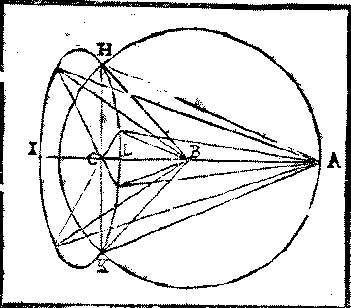
\includegraphics[max width=0.82\textwidth,max height=0.42\textheight,keepaspectratio]{images/figura03.png}\vspace{0.4em}\end{center}


\textit{Quæcunque enim ea sunt, quæ per refractionem luminis appareant verius, quàm sint; vt Iris, Corona, aliaque huiusmodi; ea semper lege producuntur, vt luminosum corpus, ex cuius existunt lumine, quocunque illud sese conuerterit, sequaci, obsentique motu consequantur. Ita iris IHL, quæ Sole existente in Horizonte A verticem sui semicirculi habet in H, si Sol intelligatur eleuari ex A vsque ad D, descendet ipsa ex opposita parte, \& verticem sui }\textit{arcus H, ad Horizontem inclinabit; \& quò altius Sol eleuabitur, eò magis Iridis vertex H deprimetur.}


\begin{center}\vspace{0.4em}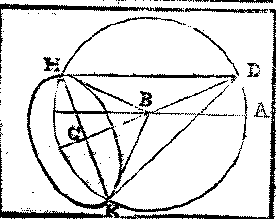
\includegraphics[max width=0.82\textwidth,max height=0.42\textheight,keepaspectratio]{images/figura04.png}\vspace{0.4em}\end{center}


\textit{Ex quo patet eamdem semper in partem Iridem moueri, in quam Sol ipse fertur.}\textit{ }\textit{Idem obseruari potest in Areis, Coronis, \& Parelijs: hæc siquidem omnia, cum luminosum, à quo fiunt, certo interuallo coronent, ad illius etiam motum in eamdem semper partem feruntur. Idem etiam apertissimè deprehenditur in imagine luminosa, quam Sol ad Occasum flectens in superficie Maris, ac fluminum formare solet. Hæc enim, quò magis à nobis Sol remouetur, eò etiam abscedit magis, donec illo occumbente euanescat. }


\begin{center}\vspace{0.4em}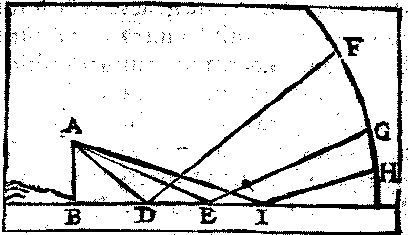
\includegraphics[max width=0.82\textwidth,max height=0.42\textheight,keepaspectratio]{images/figura05.png}\vspace{0.4em}\end{center}


\textit{Sit enim}\textit{ }\textit{superficies Maris visa BI insensibiliter à plana superficie differens; sit oculus in litore positus in A, Sol primum in F. ducantur ad D radij FD, DA, facientes angulos ADB, FDE incidentiæ, \& reflexionis, æquales in D; videbitur ergo lumen Solis in D. Descendat iam idem Sol ad G, atque eadem ratione, qua prius, ducantur à Sole G atque ab oculo A duæ lineæ facientes cum }\textit{recta BE angulos incidentiæ, \& reflexionis, æquales; hæ coincident in puncto E, \& non alio, vt est manifestum. lumen ergo Solis apparebit in E, \& propter eamdem causam, Sole magis adhuc depresso in H, lumen apparebit in }\textit{I. }\textit{Contrarium verò accidit quotiescumque idem lumen à Sole oriente in aquis producitur; tunc enim sicuti Sol magis ad verticem nostrum accedit; ita \& lumen spectanti fit propius. Prius enim v. g. apparebit in }\textit{I, }\textit{secundò in E, tertio in D. ex quibus quilibet intelligat in eam semper partem isthæc apparentia moueri, }\textit{in quam luminosa ipsa, à quibus producuntur, feruntur. Cum ergo ex Solis lumine cometa sine controuersia, producatur, Solis etiam motum sequi debuit; quod si non præstitit, inter apparentia lumina numerandus non erit. Aio igitur in cometa nihil vnquam tale obseruatum fuisse. Cum enim primo, quo visus est die, hoc est 29. Nouembris Sol in gradu Sagittarij 6. m. 43 reperiretur, atque ad Capricornum etiam tunc tenderet; necessariò singulis sequentibus diebus vsque ad 22. Decembris, in quocumque verticali depressior fieri debuit; \& si motus hic attendatur, Sol ab Aequatore magis, \& magis in Austrum mouebatur. Quare si de genere refractorum luminum, aut repercussorum fuit cometa, in Austrum etiam ferri debuit, à quo tamen motu tantum abfuit, vt in Septentrionem potius tendere voluerit. Vt fortasse, vel ex hoc, suam Galilæo testaretur libertatem, doceretque, nihil se amplius à Sole habuisse, quàm homines habeant in eiusdem Solis luce ambulantes, \& quo sua illos libido impulerit, liberè contendentes. Quòd si quis fortè hoc loco aliam aliquam reflexionis, refractionisue regulam à superioribus diuersam inuexerit, quam cometis tribuendam, nescio qua occulta prærogatiua, existimet; illud saltem statuendum est, vt quam semel admiserit motus regulam, seruet postea exactè. Sit igitur, quando hoc aliquis vult, vt libet. Fuerit cometarum non Solis motu moueri, sed contrario: vt proinde dum hic in Austrum tenderet, illi in Septentrionem aufugerent; debuerant ijdem illi, Sole ad Septentrionem redeunte, in Austrum contra, propter eamdem rationem, moueri. Cum ergo à die 22. Decembris, hoc est à Solstitio brumali, in Septentrionem iterum Sol regrederetur, debuit noster cometa in Austrum contra, vnde discesserat, remeare; hic tamen constantissimè eumdem semper motus }\textit{tenorem in Septentrionem seruauit; ex quo satis constare potest, nullam cum Solis motu cognationem habuisse incessum cometæ, cum, siue in hanc, siue in illam partem moueretur Sol, eadem ille, qua primum cœperat, semita progrederetur.}


Qual sia stato il momento de' passati trè argomenti, si è veduto sin quì; il quale credo, che anco l'istesso Sarsi non abbia reputato molto, per esser discorsi fisici, onde egli stesso nomina; e stima i seguenti presi dalle dimostrazioni ottiche di gran lunga più conchiudenti e più efficaci de' passati, indizio manifesto di non auer auuto l'intera sua soddisfazzione in quei progressi naturali. Ma auuertisca bene al caso suo, e consideri, che per vno, che si voglia persuader cosa, se non falsa, almeno assai dubbiosa, di gran vantaggio è il potersi seruire d'argomenti probabili, di conghietture, d'essempi, di verisimili ed anco di sofismi, fortificandosi appresso è ben trincerandosi con testi chiari, con autorità d'altri Filosofi, di Naturalisti, di Rettorici, e d'Istorici. Ma quel ridursi alla seuerità di Geometriche dimostrazioni è troppo pericoloso cimento per chi non le sà ben maneggiare; imperocchè, sì come \textit{ex parte rei} non si dà mezo trà il vero, e 'l falso, così nelle dimostrazioni necessarie, ò indubitabilmente si conchiude, ò inescusabilmente si paralogiza senza lasciarsi campo di poter con limitazioni, con distinzioni, con istorcimenti di parole, ò con altre girandole sostenersi più in piede, ma è forza in breui parole, ed al primo assalto restare, ò Cesare, ò niente. Questa Geometrica strettezza farà, ch'io con breuità, e con minor tedio di V. S. Illustriss. mi potrò dalle seguenti proue distrigare, le quali io chiamerò Ottiche, ò Geometriche più per secondare il Sarsi, che perche io ci ritroui dentro, dalle figure in poi molta prospettiua, ò Geometria. E, come V. S. Illustriss. vede, l'intenzion del Sarsi in questo quarto argomento di conchiudere che la cometa non sia del genere de' simulacri solamente apparenti cagionati da riflessione, e da refrazzione de' raggi solari; per la relazione, ch'ella osserua, e ritiene verso il Sole diuersa da quella, ch'osseruano, e ritengon quelle, che noi sappiamo certo esser pure apparenze, quali sono l'Iride, l'Alone, i Parelij, le reflessioni del Mare, le quali tutte, dic'egli al mouimento del Sole si vanno esse ancora mouendo con tenor tale che la mutazion loro è sempre verso la medesima parte che quella del Sole; ma nella cometa è accaduto il contrario, adunque ella non è vn'illusione. Quì, ancorchè assai competente risposta fusse il dire, che non si vede necessità veruna per la quale la cometa debba seguitar lo stile dell'Iride; ò dell'Alone o dell'altre nominate illusioni, poiche ella è differente dall'Iride, dall'Alone, e dall'altre. Tuttauia io voglio conceder qualche cosa di più dell'obligo, purche il Sarsi nel resto non voglia auer più priuilegio di mè, sihe alcun modo d'argomentare, che per lui douesse esser conchiudente, per me poi auesse da esser reputato inutile. Per tanto io domando al Sarsi, s'ei reputa l'argomento preso dalla contrarietà dello stile osseruato dalla cometa, e da i puri simulacri in contrariar quella, ed in secondar questi il moto del Sole sia necessariamente conchiudente, ò nò? s'ei risponde di nò, già tutto il suo progresso è vano, nè io più vi aggiungo parola, ma se ei risponde di sì, giusta cosa sarà, che altrettanto vaglia per mè per conchiuder, che la cometa sia vn'illusione, il dimostrar io, ch'ella osserui lo stile d'alcun vano simulacro in quel che appartiene al secondare, ò contrariare al moto del Sole. Ma per trouare tal simolacro non occorre ne anco che io mi parta da vn prodotto dall'istesso Sarsi per opportunissimo, e manifestamente farci conoscere il progresso della cometa esser contrario a quello d'esso simulacro; il quale però à mè pare non contrario, ma il medesimo à capello. Prenda dunque V. S. Illustriss. la sua seconda figura, nella quale ei fà parallelo della cometa con la reflession del Sole fatta nella superficie del Mare, doue, quando il Sole sia in H. il suo simulacro vien veduto dall'occhio A. secondo la linea AI. E quando il Sole sarà in G. si vedrà il simulacro per la linea AE. ed essendo in F. il simulacro apparrà nella linea AD. Resta ora che veggiamo, mentre che il Sole ci apparisce essersi mosso in Cielo per l'arco HGF. per qual verso ci apparisca essersi mosso parimente il suo simulacro, rispetto al Cielo, doue il Sarsi osseruò il moto della cometa, e del Sole, perloche bisogna continuar l'arco FGHLMN. e prolungar le linee AI. AE. AD. in L. M. N. e poi dire:


\begin{center}\vspace{0.4em}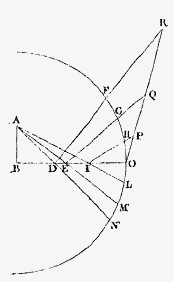
\includegraphics[max width=0.82\textwidth,max height=0.42\textheight,keepaspectratio]{images/figura06.png}\vspace{0.4em}\end{center}


Quando il Sol era in H. il suo simulacro si vedeua per la linea AI. che in Cielo risponde nel punto L. e quando il Sole venne in G. il suo simulacro si vedeua per la linea AE. ed appariua in M. e finalmente, giunto il Sole in F. il suo simolacro apparse in N. Adunque, mouendosi il Sole da H. verso F. il suo simolacro apparisce muouersi da L. in N. ma questo, S. Sarsi, è apparir muouersi al contrario del Sole, e non pel medesimo verso, come auete creduto, ò più tosto voluto dare à creder voi. Io, Illustriss. S. dico così, perche non mi posso persuadere, com'egli auesse auuto à equiuocare in cosa tanto manifesta: oltre che si vede anco, che nel dichiararsi vsa certe maniere di dire assai improprie, e non consuete, solo per accommodare al suo bisogno quello, ch'accommodar non vi si può, perche non è nulla v. g. ei si vede, che passando il Sole da H. in G. e da G. in F. la sua immagine viene da I. in E. e da E. in D. il qual progresso IED. è vn vero, e realissimo auuicinarsi, e muouersi verso l'occhio A. E perche il bisogno del Sarsi è di poter dir, che l'immagine, ed il Sole si muouano pel medesimo verso, ei si risolue liberamente à dire, che 'l moto del Sole per l'arco HGF. sia vn'auuicinarsi al punto A. e che l'andar verso il vertice, sia il medesimo, che andar verso il centro. E di più forza, ch'ei dissimuli di non s'accorgere d'vn'altro più graue assurdo, che gli verrebbe addosso quand'ei volesse sostenere, che il simulacro secondasse il mouimento dell'oggetto reale; perche quando questo fusse; bisognerebbe di necessità, che parimente pel conuerso, l'oggetto secondasse il simulacro; dal che vegga V. S. Illustriss. quel che ne seguirebbe. Tirisi dal termine del diametro O. la linea retta OR. cadente fuor del cerchio e colla BO. contenente qualsiuoglia angolo, e si prolunghino sino ad essa le DF. EG. IH. ne i punti R. Q. P. è manifesto, che quando l'oggetto reale si fusse mosso per la linea P. Q. R. il simulacro sarebbe venuto per la I. E D. e perche questo è vno auuicinarsi e muouersi verso l'occhio A. e quel, che fà il simulacro, lo fà ancora (per detto del Sarsi) l'oggetto; adunque l'oggetto, mouendosi dal termine P. in R. si è venuto auuicinando al punto A. ma egli si è discostato. Ecco dunque l'assurdo manifesto. Notisi di più, che quanto il Sarsi và considerando in questo luogo accader trà l'oggetto reale, e la sua immagine, è preso come se la materia, in cui si deue formare il simulacro resti sempre immobile, e solo si muoua l'oggetto; che quando s'intendesse muouersi detta materia ancora, altre, ed altre conseguenze ne seguirebbono circa l'apparenze del simulacro: e però da quel, che aggiunge il Sarsi, del non esser ritornata indietro la cometa al ritorno del Sole, non se ne inferirà mai nulla, se prima non si determina dello stato o del mouimento della materia in cui la cometa si produsse.



\par\bigskip\noindent\phantomsection\addcontentsline{toc}{section}{§ 25}{\Large\color{rubric}\textbf{25.}}\enspace Passo al quinto argomento. \textit{Præterea, si de apparentium simulacrorum numero cometa fuit, debuit ad certum ac determinatum angulum spectari, quod in Iride, Area, Corona, alijsque huiusmodi accidit. Meminisse autem hoc loco debet Galilæus, se affirmasse satis amplum Cæli spatium huiusmodi vaporibus occupatum: quod si ita est; aio circularem, vel circuli segmentum apparere cometam debuisse. Sic enim argumentari libet. Quæcumque sub vno certo, ac determinato angulo conspiciuntur, ibi videntur, vbi certus ille, ac determinatus angulus constituitur, sed pluribus in locis in circulari linea positis, determinatus hic, \& certus cometæ angulus constituitur; ergo pluribus in locis, in linea circulari dispositis cometa videbitur. maior certissima est, neque vllius probationis indigens. Minorem sic probo.}


\begin{center}\vspace{0.4em}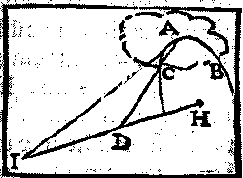
\includegraphics[max width=0.82\textwidth,max height=0.42\textheight,keepaspectratio]{images/figura07.png}\vspace{0.4em}\end{center}


\textit{Sit sol infra Horizontem in }\textit{I, }\textit{locus vaporis fumidi circa A, cometa vero ipse se se, v. g., spectandum ostendat in A, posito oculo in D. occupet autem vapor idem \& alias partes circa A constituas, quod Galilæus vltrò concedit. Intelligatur iam ducta linea recta per centrum Solis }\textit{I, }\textit{\& per centrum visus D. ex punctis vero }\textit{I, }\textit{\& D ad locum cometæ A concurrant radij IA, DA, constituentes triangulum IAD. erit ergo angulus IAD ille certus, \& determinatus, sub quo ad nos cometæ species remittitur. Concipiamus iam circa axem IDH triangulum IAD moueri, tunc vertex illius A describet segmentum circuli, in quo semper radij Solis, IA directus, \& AD reflexus angulum eundem IAD efficient: cum autem in hac verticis A circumductione multæ ab illo circumfusi vaporis partes attingantur, in ijs omnibus fiet determinatus ille, ac certus angulus, ad quem cometa necessariò consequitur: in toto ergo circuli segmento BAC, quod vaporem attingit, cometa comparebit; eadem prorsus ratione, qua in roridis nubibus Irides, \& Coronas fieri contingit, aut circulares, aut circulorum segmenta. Cum }\textit{ergonihil tale in cometa obseruatum fuerit, non erit proindè in apparentium simulacrorum numero collocandus; cum nulla in re hic illis se similem præbeat.}


Seguita, anzi pur cresce, in mè la merauiglia nata dal veder quanto frequentemente il Sarsi vada dissimulando di vedere le cose, ch'egli hà dinanzi agli occhi con speranza forse, che la sua dissimulazione abbia negli altri à partorire non vna simulata, ma vna vera cecità. Ei vuole nel presente suo argomento prouar, che quando la cometa fusse vna nuda apparenza, ella dourebbe dimostrarsi in figura di cerchio, ò di parte di cerchio, perche così auuiene dell'Iride, dell'Alone, della Corona e dell'altre varie immagini, il che non sò, com'ei possa affermare, sendosi cento volte ricordata la reflession nel mare dell'immagine solare, e quelle proiezzioni dall'aperture delle nuuole, le quali compariscono strisce dritte, e similissime alla cometa. Ma forse ei si persuade, che senz'altre auuertenze la dimostrazione ottica, ch'ei n'arreca, conchiuda nella cometa necessariamente la sua intenzione; delche però io grandemente dubito, e parmi, s'io non m'inganno, che 'l suo progresso sia mutilo, e che gli manchi vna parte principalissima del dato (che sarebbe gran difetto in Logica) e questa è la disposizion locale in relazione all'occhio della superficie di quella materia, nella quale si hà à far la riflessione, la qual disposizione non vien messa in considerazion dal Sarsi, di che non saperei addur più modesta scusa, che il non l'auere egli auuertito; chè quando ei l'auesse conosciuto, ma dissimolato per mantenere il Lettore nell'ignoranza, mi parrebbe mancamento assai più graue. La considerazion poi di cotal disposizione opera il tutto; imperocchè la dimostrazion del Sarsi non conchiuderà mai, se non quando la superficie del vapore intorno al punto A. della sua figura sarà opposta all'occhio D. direttamente, sì che l'asse IDH. caschi perpendicolarmente sopra il piano, nel quale essa superficie si distendesse; perche allora nel girare il triangolo IDA. intorno all'asse IH. il punto A. anderebbe terminando continouamente in essa superficie, e descriuendoui vna circonferenza di cerchio, chè quando la superficie detta fusse esposta all'occhio obliquamente, l'angolo A. non la toccherebbe, se non in vn sol punto, e nel girar del triangolo, il medesimo angolo A. ò penetrerebbe oltre ad essa superficie, ò non v'arriuerebbe. Ed in somma à voler, che la cometa apparisse circolare, bisognerebbe che la superficie, dou'ella si genera fusse piana, \& esposta direttamente alla linea, che passa per li centri dell'occhio, e del Sole; la qual constituzione non può mai accadere, se non nella diametrale opposizione, ouero nella linear congiunzione de' vapori, e del Sole: e però l'Iride si vede sempre opposto, l'Alone ò la corona sempre congiunti al Sole, onde appariscono circolari; ma delle comete non sò che se ne sien mai vedute, nè in opposizione, nè in congiunzione al Sole. Se al Sarsi nello scriuere la sua dimostrazione fusse vna volta passato per la fantasia di chiamar quella materia, ch'ei si figura intorno al punto A. non vapori, ma acqua del Mare, ei si sarebbe accorto, che 'l suo argomento aurebbe nel modo stesso, e coll'istesse parole concluso, che la riflessione nel Mare di necessità si deue distender per linea circolare; dalche poi mercè del senso, che mostra il contrario, aurebbe scoperta la fallacia del suo sillogismo.



\par\bigskip\noindent\phantomsection\addcontentsline{toc}{section}{§ 26}{\Large\color{rubric}\textbf{26.}}\enspace Or sentiamo l'argomento sesto: \textit{Sed placet, ex ipsius etiam Galilæi verbis, hoc idem confirmare. Ait enim ipse; quod etiam fortasse verissimum est, spectra huiusmodi, \& }\textit{vana simulacra eam in Parallaxi legem seruare, quam seruat luminosum illud corpus, à quo proueniunt. Ita, si qua illorum Lunæ effecta fuerint, hæc parem cum Luna Parallaxim pati; quæ verò à Sole fiunt, eamdem cum Sole aspectus diuersitatem sortiri. }\textit{Prætereà, dum aduersus Aristotelem disputat, \& argumentum ex Parallaxi ductum assumit, hæc habet. Denique cometam ignem esse, ac sublunarem asserere omninò impossibile est, cum obstet Parallaxis exiguitas, tot insignium Astronomorum solertissima inquisitione, obseruata. Ex quibus ita rem conficio. Auctore Galilæo, quæcumque merè apparentia, à Sole producuntur, illa eamdem patiuntur Parallaxim. quam patitur Sol; sed cometa non passus est eamdem Parallaxim, quam Sol patitur; ergo cometa non est apparens quid à Sole productum. Si quis autem de minori huius argumenti propositione ambigat; Tychonis obseruationes cum obseruationibus aliorum conferat, dum agunt de cometa anni 1577. Ipse certè Tycho ex suis obseruationibus illud tandem deducit; demonstratam nimirum distantiam Cometæ à centro Terræ, die 13. }\textit{Nouembris fuisse semidiametrorum eiusdem Terræ. 211. tantum, cum Sol ab eodem centro }\textit{ponatur distare semidiametris saltem 1150. Luna vero semidiametris 60. De hoc verò nostro, si quis eas obseruationes inter se contulerit, quas in disputatione ab vno ex Patribus habita, edidit in lucem Magister meus; satis illi inde costabit huius propositionis veritas. Nam ferè semper longè maiorem cometæ Parallaxim inueniet, quàm Solis. Neque obseruationes huiusmodi Galilæo suspectæ esse nunc possunt, cum easdem summorum Astronomorum opera exquisitissimè ad Astronomiæ calculos castigatas testatus sit.}


Che il S. M. ed io abbiamo mai scritto, ò detto, che i simolacri prodotti dal Sole ritengano la medesima Paralasse che quello (come il Sarsi in questo luogo afferma per fondamento del suo sillogismo) è del tutto falso; anzi il S. M. dopò auer nominati, e considerati molti de' tali simolacri, soggiugne così. \textit{E auuenga che de' sopranominati simolacri in alcuni la Paralasse sia nulla, ed in altri operi molto diuersamente da quello, ch'ella fà negli oggetti reali}. Non si troua nella scrittura del S. M. ch'egli affermi, la Paralasse esser l'istessa, che quella del Sole, ò della Luna, se non nell'Alone; negli altri, \& anco nell'istesso Iride, vien posta diuersa. Falsa dunque è la prima proposizion del sillogismo. Or veggiamo quanto sia vera la seconda, e quanto conchiudente, posto anco, che la Paralasse di tutti i simolacri vani douesse essere eguale à quella del Sole. Vuole il Sarsi, e coll'autorità di Ticcone, e con quella del suo Maestro, prouare (e così è in obligo di fare) che la Paralasse osseruata nelle comete sia maggiore di quella del Sole. Ma s'astiene poi di proddurre l'osseruazioni particolari di Ticcone, e di molti altri Astronomi di nome, fatte circa la Paralasse della cometa; e ciò fa egli, perche il Lettore non vegga come quelle sono trà di loro differentissime, e qualunque elle si sieno, ò sono giuste, ò sono errate; se giuste, si che à loro si debba prestare intera fede, bisogna necessariamente conchiudere, ò che la medesima cometa fusse nell'istesso tempo, e sotto il Sole, e sopra, ed anco nel firmamento, ò vero, che, per non essere ella vn'oggetto fisso, e reale, ma vago, e vano, non soggiace alle leggi dei fissi, e reali; ma se tali osseruazioni sono errate, mancano d'autorità, nè per esse si può diterminar cosa veruna, e l'istesso Ticcone trà tante diuersità andò eleggendo, come se fussero più certe quelle che più seruiuano alla sua determinazione fatta innanzi di voler assegnar luogo alla cometa trà il Sole, e Venere. Quanto poi all'altre osseruazioni proddotte dal suo Maestro, sono tanto frà se differenti, ch'egli medesimo le determina inette à potere stabilire il luogo della cometa, dicendo quelle esser state fatte con istrumenti non esatti, e senza la necessaria considerazion dell'ore, e della refrazzione, e d'altre circostanze perloche egli stesso non obliga altrui à prestargli molta fede, ma si riduce ad vna sola osseruazione, la quale non ricercando strumento alcuno, ma potendo colla semplice vista farsi esattissimamente, egli l'antepone à tutte l'altre, e questa fù la puntual congiunzione del capo della cometa con vna stella fissa, la qual congiunzione fù vista nel medesimo tempo da luoghi trà di se molto distanti. Ma, S. Sarsi, se così è seguito questo è del tutto contrario al bisogno vostro, poiche di quì si raccoglie, la Paralasse essere stata nulla, mentre che voi prodducete questa auttorità per confermar la vostra proposizione, che dice tal Paralasse esser maggiore che quella del Sole. Or vedete come gli stessi Autori chiamati da voi testificano contro alla causa vostra. A quello poi, che voi dite, che noi stessi abbiamo confessato l'osseruazione degli Astronomi grandi, essere state fatte esattissimamente; vi rispondo; che se voi meglio considererete il doue, e 'l quando sono state chiamate tali, comprenderete, che esatte si poteuano dire, quando elle fussero state anco assai più differenti trà loro di quello, che state sono. Furon chiamate esatte, e sufficienti à confutar l'opinione di Arist. mentr'egli voleua, che la cometa fusse oggetto reale, e vicinissimo alla Terra; e non sapete, che il vostro Maestro stesso dimostra, che il solo interuallo trà Roma, ed Annuersa in vn'oggetto reale che, fusse anco sopra la suprema region dell'aria, può cagionar Paralasse maggiore di 50. di 60. di 100. ed anco di 140. gradi? e se questo è non si potranno elleno chiamar osseruazioni esatte, e potenti quelle, che, essendo tutte minori d'vn grado solo differiscono trà di loro di pochi minuti



\par\bigskip\noindent\phantomsection\addcontentsline{toc}{section}{§ 27}{\Large\color{rubric}\textbf{27.}}\enspace Or legga V. S. Illustriss. l'vltimo argumento. \textit{Denique neque illud omittendum, quod vel vnum homini veritatis potius inuestigandæ, quàm altercandi cupido, satis, id quod agimus persuadere possit. Experimur enim quotidie, ea omnia, quibus certa, ac stabilis species non est, sed vana colorum, ac lucis imagine, illudunt oculis, angustissimis vitæ spatijs finiri, breuissimo etiam temporis interuallo, varias sese in formas mutare; modò extingui, modò iterum accendi; nunc pallescere, nunc ardentiori luce micare, partes illorum nunc interrumpi, nunc iterum coalescere, nunquam denique eadem diu specie apparere, quæ omnia, si cometæ stabili motu, aspectuque conferantur, ostendent, quanta demum inter illum, atque huiusmodi vanas imagines morum, ac Naturæ discordia sit. Quare si nihil planè reperias, in quo se illis cometa similem probet; cur non potius, nullam cum ijsdem Naturæ affinitatem, aut cognationem habere dixeris? Dixerunt enimuerò Philosophorum antiquissimi, atque optimi, dixerunt recentiorum eruditissimi: vnus nunc Galilæus illis repugnat, at Galilæo, nisi fallor, repugnare veritas videtur.}


Il qual argomento egli stima tanto, che gli par, ch'esso solo possa esser bastante à persuader l'intento suo; tuttauia io non ci scorgo efficacia, che mi persuada, mentr'io considero, che nel proddur questi vani simulacri v'interuiene il Sole, com'efficiente, e le nuuole e vapori, ò altre cose, come materia; e perche l'efficiente è perpetouo, quando non mancasse dalla materia, e l'Iride, e l'Alone, ed i Parelij, e tutte l'altre apparenze sarebbono perpetoue; la breue dunque, ò lunga durazion dalla stabilità, e posizion della materia si deue attendere. Or qual ragione ci dissuade poter esser sopra le regioni elementari alcuna materia di più lunga durazione delle nubi, della caligine, della pioggia cadente in minute stille, ò d'altre materie elementari, siche la riflessione, ò refrazzion del Sole fatta in quelle ci si mostri più lungamente dell'Iride, de' Parelij, dell'Alone? ma senza partirsi da' nostri elementi; l'Aurora, ch'è vna refrazzion de' raggi solari nella region vaporosa, e le riflessioni nella superficie del Mare non son'elleno apparenze perpetoue, siche se il riguardante, il Sole, i vapori, e la superficie del Mare stessero sempre nella medesima disposizione, perpetouamente si vederebbe l'Aurora, e la striscia splendida nell'acqua? In oltre dalla minore, ò maggior durazione, poco conchiudentemente s'inferisce vn'essenzial differenza, anzi delle comete stesse, senza cercar altre materie, se ne son vedute alcune durare 90. e più giorni, ed altre dissoluersi il quarto, ed anco il terzo. E perche si è osseruato, le più diuturne mostrarsi anco nel lor primo apparire, assai maggiori dell'altre, chi sà che non ve ne sieno, ed anco frequentemente, di quelle, che durino non solamente pochi giorni, ma anco non molte ore, ma che per la lor piccolezza non vengano facilmente osseruate? E per conchiuderla, che nel luogo doue si formano le comete vi sia materia atta nata à conseruarsi più della nuuola, e della caligine elementare, l'istesse comete ce n'assicurano, prodducendosi di materia, ò in materia non celeste, ed eterna, nè anco che necessariamente in breuissimi tempi si dissolua; si che il dubbio resta ancora, se quello che si prodduce in detta materia sia vna pura e semplice reflession di lume, ed in conseguenza vno apparente simulacro, ò pure se sia altra cosa fissa e reale; E per tanto niuna cosa conchiude l'argomento del S. Sarsi, nè conchiuderà, s'egli prima non dimostra, che la materia cometaria non sia atta à riflettere, ò rifrangere il lume solare, perche quanto all'esser atta à durar molti giorni, la durazion delle medesime comete ce ne rende più che certi.



\par\bigskip\noindent\phantomsection\addcontentsline{toc}{section}{§ 28}{\Large\color{rubric}\textbf{28.}}\enspace Or passiamo alla seconda questione di questo secondo essame. \textit{Venio nunc ad motum: quem rectum fuisse Galilæus asserit, ego tamen disertè nego. Ea primùm ratio, hoc mihi persuadet vt faciam, quàm ipse soluere, vel nescire se, vel non audere ingenuè profitetur. Illa enim ratio adeò aperta est, adeòque ad hunc motum dissuadendum efficax, vt cum fortè id maximè vellet, dissimulare}\textit{ tamen eam non potuerit. Si enim }(\textit{verba eius sunt})\textit{ solus hic motus cometæ tribuatur, explicari non potest, quì factum sit, vt non ad verticem solum magis ac magis accesserit, sed vlterius, ad Polum vsque peruenerit quare vel præclarum hoc inuentum abijciendum, quod sanè haud sciam, vel motus alius addendus,}\textit{ }\textit{quod non ausim. Vbi mirandum sanè est, hominem apertum, ac minimè meticulosum, repentino adeò timore corripi, vt conceptum sermonem proferre non audeat. Ego verò non is sum, qui diuinare norim.}


E quì prima ch'io proceda più auanti, non posso far ch'io non mi risenta alquanto col Sarsi della non punto meritata imputazione, ch'egli m'attribuisce di dissimolatore, essendo cotal nota lontanissima dalla profession mia, la qual è di liberamente confessare come sempre hò fatto, di ritrouarmi abbagliato e quasi del tutto cieco nel penetrare i secreti di Natura, ma ben d'esser desideratissimo di conseguir qualche piccola cognizione d'alcuno d'essi, alla quale intenzione niun'altra cosa è più contraria, che la finzione, ò dissimulazione. Il Sig. M. nella sua scrittura mai non hà finto cosa alcuna, nè hà auuto di mestieri di fingerla, poiche quanto egli di nuouo hà proposto l'hà portato sempre dubitatiuamente, e conghietturalmente, nè hà cercato di fare ad altri tener per certo, e sicuro quello, ch'egli, ed io per dubbio, ed al più per probabile abbiamo arrecato, ed esposto alla considerazion de' più intelligenti di noi, per trarne, co 'l loro aiuto, ò la confermazione di alcuna conchiusion vera, ò la totale esclusion delle false. Ma se la scrittura del S. M. è schietta, e sincera, ben altrettanto è piena di simolazioni la vostra S. Lottario; poiche, per farui strada alle oppugnazioni delle 10. volte le 9. fingete di non intendere quel, che hà scritto il S. M. e dandogli sensi molto lontani dall'intenzion di quello, e spesso aggiungendoui, ò leuandone, preparate ad arbitrio vostro la materia, onde il Lettore prestando fede à quanto voi prodducete poi in contrario resti in concetto, che noi abbiamo scritte gran semplicità, e che voi acutamente l'auete scoperte, e ributtate, il che sin quì si è da me osseruato, e nel restante s'osseruerà non meno. Ma venendo al fatto, qual cagione vi muoue à scriuere, che noi abbiamo sommamente voluto, ma non potuto dissimolare, che mouendosi la cometa di semplice moto retto, fusse necessario, ch'ella andasse sempre verso il vertice, ne da quello declinasse giamai? chi hà fatto auuertito voi di tal conseguenza, altri che l'istesso S. M. che la scriue; la quale al sicuro à voi aurebbe egli potuto dissimulare, e voi per vostra benignità auereste dissimolata la sua dissimolazione. Ma che più? voi stesso due solli versi di sopra scriuete, che io ingenuamente hò confessato di non sapere, ò non ardir di sciorre cotal ragione da mè prodotta, ed accanto, accanto soggiungete, ch'io massimamente aurei voluto dissimolarla, e qual contradizzion'è questa, che vno ingenuamente porti, e scriua, e stampi vna proposizione, e sia il primo à portarla, e scriuerla, e stamparla, e che voi poi diciate lui auer grandemente disiderato di dissimolarla, ed asconderla? veramente, S. Lottario, voi siete molto bisognoso, che nel Lettore sia vna gran semplicità, ed vna piccola auuertenza. Or veggiamo se in questo detto, doue nulla si troua di nostra simolazione, ve ne fusse per sorte di quella del Sarsi. E certo in poche parole ven'è più d'vna, e prima, per aprirsi il campo à dichiararmi per tanto ignorante Geometra, che non abbia capito quelle conseguenze che per lor dimostrazione non ricercano maggiore scienza, che di alcune poche, e tritissime proposizioni del primo libro degli elementi, egli mi fà dir quello, che già mai non s'è detto, nè scritto; e mentre noi diciamo, che se la cometa si mouesse di moto retto, ci apparrebbe muouersi verso il vertice, e zenit, esso vuole che noi abbiamo detto ch'ella, mouendosi douesse arriuare al vertice, e zenit. Quì bisogna che il Sarsi confessi, ò di non auere inteso quel, che vuol dir \textit{muouersi verso vn luogo}, ò d'auer voluto con finzione, e simolazione attribuirci vna falsità; Il primo non credo, che possa essere, perche così verrebbe anco à stimare, che il dir \textit{nauigare verso il Polo,} e \textit{tirar vna Pietra verso il Cielo} importasse che la naue arriuasse al Polo, e la Pietra in Cielo. Adunque resta, ch'egli dissimolando d'intender il vero scritto da noi, ci attribuisca il falso per poter poi attribuirci le non meritate note. Di più non sinceramente riferisce egli le presenti parole del S. M. anco in vn'altro particolare; poiche doue quello dice, che ò bisogna rimuouere il moto retto attribuito alla cometa, ò vero, ritenendolo, aggiungere qualche altra cagione dell'apparente deuiazione; il Sarsi di suo arbitrio muta le parole. \textit{Qualche altra cagione,} in \textit{qualch'altro moto}, per poter poi, fuor d'ogni mia intenzione tirarmi nel moto della Terra, e quì scriuer varie girandole, e vanità; conchiuda finalmente il Sarsi non esser di quelli, che sanno indouinare; e pure assai frequentemente si getta al voler penetrare gl'interni sensi altrui.



\par\bigskip\noindent\phantomsection\addcontentsline{toc}{section}{§ 29}{\Large\color{rubric}\textbf{29.}}\enspace Or segua V. S. Illustrissima. \textit{Quæro igitur, an motus hic alius, quo bellè explicare omnia posset, nec eum proferre audet, vapori huic cometico, tribuendus sit, an alij cuipiam, ad cuius postea motum moueri, in speciem tantùm, videatur cometa. Non primum, arbitror, hoc enim esset motum illum rectum, \& perpendicularem destruere; siquidem, si vapor ex terra, Aequatori verbi gratia subiecta, motu perpendiculari sursum ascendat, \& motu alio idem ipse in Septentrionem feratur; motus hic secundus necessariò priorem destruet: quòd si nihilominus ad Septentrionem moueri, saltem in speciem, videatur; ad alterius alicuius corporis motum, id consequi, dicendum erit. Certè dvm Galilæus ait, eum motum qui addendus esset, causam tantummodò futurum apparentis deuiationis cometæ; satis apertè innuit, motum hunc in alio, quàm in vapore cometico ponendum esse; cum illum apparenter solùm ad Septentrionem moueri velit. }\textit{Quod si ita est, non video, cuiusnam corporis hic futurus sit motus. Cum enim nulli Galilæo sint Cælestes Ptolemæi orbes, nihilque ex eiusdem Galilæi Systemate, in Cælo solidi inueniatur; non igitur ad motum eorum orbium, quos nusquam reperiri existimat, cometam moueri putabit. }\textit{Sed audio hic mihi nescio quem tacitè, ac timidè in aurem insusurrantem Terræ }\textit{motum. Apage dissonum veritati, ac pijs auribus asperum verbum. Næ tu cautè id submissa insusurrasti voce. sed si ita res se haberet, conclamata esset Galilæi opinio, quæ non alij, quam huic falso inniteretur fundamento. Si enim Terra non moueatur, motus hic rectus cum obseruationibus cometæ non congruit; sed Terram, certum est apud Catholicos, non moueri; erit ergo æquè certum, motum hunc rectum cum obseruationibus cometicis minimè concordare, ac propterea ineptum ad rem nostram iudicandum. neque id ego vnquam Galilæo in mentem venisse existimo, quem pium semper, ac religiosum noui.}


Qui, com'ella vede, si va il Sarsi affaticando per mostrar, niun altro moto, che si attribuisca, ò all'istessa cometa, ò ad altro corpo mondano poter esser'atto à mantenere il mouimento per linea retta, introdotto dal S. M. ed à supplire insieme all'apparente deuiazion dal vertice, il qual discorso è tutto superfluo, e vano, atteso che nè il S. M. nè io abbiamo mai scritto, la cagion di tal deuiazione depender da qualch'altro moto, nè di Terra nè di Cieli nè d'altro corpo. Il Sarsi di suo capriccio l'ha introdotto, egli stesso si risponda, nè pretenda d'obligar altri à sostener quello, che non hà detto, nè scritto, nè forse pensato, ancor per confessione dell'istesso Sarsi, il quale apertamente afferma di non creder che mai mi sia caduto in mente d'introdurre il mouimento della Terra per saluar tal deuiazione, auendomi egli conosciuto sempre per persona pia, e religiosa; ma s'è così; à che proposito l'auete voi nominato, ed à qual fine cercato di mostrarlo inetto à cotal bisogno? Ma è bene che passiamo auanti.



\par\bigskip\noindent\phantomsection\addcontentsline{toc}{section}{§ 30}{\Large\color{rubric}\textbf{30.}}\enspace Segua, dunque, V. S. Illustriss. di leggere. \textit{Verùm, ni fallor, non quilibet cometæ motus Galilæum torsit, coegitque }\textit{aliquid aliud prætereà excogitare, quod proferre, vel nesciat, vel non audeat; sed is tantum, quo vltra nostrum verticem, seu Zenith, propius ad Polum accessit. Si igitur vltra verticem cometa progressus non fuisset, nil erat, quòd de hoc alio motu cogitaret. Hoc enim ipsemet verbis illis innuere videtur, quibus ait; si nullus alius ponatur motus, quàm rectus, ac perpendicularis, tunc ad nostrum tantùm verticem, rectà cometam ascensurum, non tamen progressurum vlterius.}


\begin{center}\vspace{0.4em}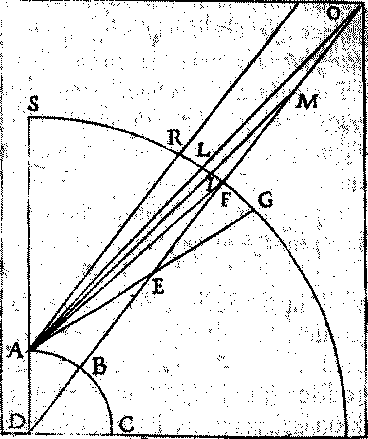
\includegraphics[max width=0.82\textwidth,max height=0.42\textheight,keepaspectratio]{images/figura08.png}\vspace{0.4em}\end{center}


\textit{Demus igitur, nullum vnquam Cometam verticem nostrum prætergressum. aio tamen, ne sic quidem, eius cursum explicari posse motu hoc recto. Sit enim Terræ globus ABC, locus, ex quo vapor ascendit sit B, oculus verò spectantis in A, visusque sit primum cometa, v. g., in E, locus eidem respondens in Cælo sit G. Intelligatur moueri cometa }\textit{sursum in linea BO per partes æquales EF, FM, MO. Affirmo quantumuis vapor ille per lineam DO ascendat, etiam in omni æternitate, nunquam ad verticem nostrum, nè apparenter quidem, peruenturum. Ducatur enim linea AR ipsi BO parallela: nunquam tantus erit cometæ motus apparens, quantus est arcus GR, \& nunquam radius visualis coincidet cum linea AR. Cum enim semper radius visiuus concurrere debeat cum recta BO, in qua apparet cometa, cumque radius AR sit lineæ BO parallelus; non poterit cum illa vnquam concurrere, ex definitione parallelarum: ergo nunquam radius, per quem cometa videtur, poterit ad R peruenire; \& consequenter, motus apparens cometæ, non solum non perueniet ad nostrum verticem S, sed neque ad punctum R, quod longissimè adhuc à vertice distat. Apparebit enim primo in G. secundo in F. tertio in }\textit{I. }\textit{deinde in L. \&c. sed nunquam perueniet ad R.}


Torna il Sarsi, come V. S. Illustriss. vede, ad alterar la scrittura del S. M., volendo pure, ch'egli abbia scritto, che il moto perpendicolare alla Terra douesse condur finalmente la cometa al punto verticale; il che non si troua nel suo libro; ma sì bene che tal moto sarebbe verso il vertice, e ciò fa, per mio parere il Sarsi, per pigliare occasione di portarci questa geometrica dimostrazione, fabbricata sopra fondamenti non più profondi della sola intelligenza della diffinizione delle linee parallele, dalla quale azzione alcuno potrebbe dedurre forse vna conseguenza non molto insigne pel Sarsi; imperocchè, ò egli stima questa sua conchiusione, e dimostrazione per cosa ingegnosa, e da persone non vulgari, ò vero per vna cosuccia da essere anco ritrouata da' fanciulli. S'egli la stima per cosa puerile, poteua ben'esser sicuro, che nè il S. M. ned io siamo costituiti in sì infelice stato di cognizione, che per mancamento di cotal notizia auessimo ad incorrere in errore; ma se ei l'hà per cosa sottile, e di momento, io non saperei come non far giudicio ch'ei fusse pouero affatto, e bisognoso di ritornar sotto la disciplina del Mæstro. E vero dunque, che il moto perpendicolare alla superficie terrestre non arriua mai al vertice (eccetto però, che quello, che si parte dall'istesso luogo del riguardante, il che forse il Sarsi non hà osseruato), ma è anco vero che noi non abbiamo detto mai ch'ei v'arriui.



\par\bigskip\noindent\phantomsection\addcontentsline{toc}{section}{§ 31}{\Large\color{rubric}\textbf{31.}}\enspace \textit{Præterea, quoniam, vt Galilæus ipse fatetur, cometæ motus in principio velocior visus est, \& paulatim postea remitti. Videndum est, in qua proportione hæc motus remissio procedere debeat in hac linea recta. Certè si Galilæi figuram expendamus, quando cometa fuerit in E, apparebit in G; cum verò, paria percurrens spatia EF, FM, MO, motum suum apparentem in punctis F}\textit{I}\textit{L ostendet; videbitur motus eius decrescere decrementis maximis; nam arcus FI vix est medietas ipsius GF, \& IL ipsius FI, atque ita de reliquis; debuit ergo cometæ motus apparens in eadem proportione decrescere. Sciendum autem est, motum cometæ osseruatum non in hac proportione decreuisse; immò primis diebus adeo exiguum ipsius decrementum fuisse, vt non facilè animaduerteretur. }\textit{Cum enim in suo exordio tres circiter gradus quotidie percurreret, diebus iam 20. elapsis, vix quicquam de illa priori contentione remisisse visus est. Immò, si in iudicium aduocentur cometæ duo Tychonici annorum 1577. \& 1585. ex ipsorum motibus apertissimè colligemus, quàm longè abfuerint ab immani hoc decremento. Si quis iam ex me quærat, quantus tandem futurus sit cometæ motus per lineam hanc rectam ascendentis. Respondeo, si cometa tunc primùm appareat, }\textit{cum vapor, ex quo producitur non longè abest à Luna, quod valdè probabile est, \& præterea ponamus locum, ex quo in Terræ globo fumus ille ascendit, distare à nobis gradibus 60. respondeo inquam, apparentem cometæ motum, toto durationis suæ tempore non absoluturum gradum vnum, \& min.}


\begin{center}\vspace{0.4em}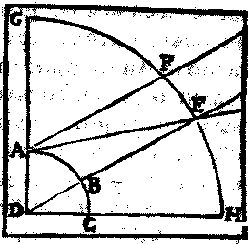
\includegraphics[max width=0.82\textwidth,max height=0.42\textheight,keepaspectratio]{images/figura09.png}\vspace{0.4em}\end{center}


\textit{31. Sit enim Terræ globus ABC. Lunæ concauum GFH distans à centro D. Terræ semidiametris 33. ex Ptolemæo; Tycho enim duplam ferè ponit distantiam, quod magis è re mea foret. }\textit{Sitque A locus, ex quo spectatur cometa, B verò locus, ex quo vapor ascendit. Dico, cum visus fuerit cometa in E, futurum angulum DEA grad. }\textit{1. min. 31. ac proinde, si ducatur AF parallela ipsi DE, erit etiam angulus FAE grad. 1. min. 31. cum sit alternus ipsi DAE inter easdem parallelas; duæ ergo lineæ AE, AF intercipient in Firmamento arcum gr. 1. min. 31. sed ad lineam AF, }\textit{parallelam ipsi DE, nunquam perueniet cometa, vt probauimus superius: ergo nunquam absoluet motum grad. 1. min. 31. Quòd autem angulus DEA futurus sit in concauo Lunæ grad. 1. min. 31. probatur; quia cum cognitus sit, ex suppositione, angulus EDA graduum 60. in triangulo ADE, \& præterea latus AD vnius Terræ semidiametri, \& latus DE semidiam. 33. si fiat, vt 34. aggregatum duorum laterum AD, DE, ad 32. differentiam eorumdem laterum, ita 173205. tangens dimidij summæ reliquorum duorum angulorum, hoc est tangens anguli grad. 60. ad quartum numerum, inuenietur 163016. tangens anguli grad. 58. min. 29. qui, detracti ex grad. 60. hoc est, ex dimidio duorum reliquorum angulorum, relinquent angulum DEA quæsitum gra. 1. min. 31. ex regulis trigonometricis.}


Io credetti dalla precedente dimostrazion del Sarsi, ch'ei potesse essere ch'egli auesse veduto, e forse inteso, il primo libro degli Elementi della Geometria; ma quello ch'egli scriue qui, mi mette in gran dubbio, s'egli abbia prattica veruna sopra le cose matematiche, poiche dalla figura delineata di sua fantasia da sè medesimo, ei vuol ritrarre qual sia la proporzion della diminuzion dell'apparente velocità del moto attribuito dal S. M. alla cometa: doue prima egli dimostra di non auere osseruato, che in tutti i libri de' Matematici niun riguardo si hà già mai delle figure, tutta volta, che vi è la scrittura che parla, e che in Astronomia, in particolare, si tratterebbe poco meno, che dell'impossibile à voler mantenere nelle figure le proporzioni, che realmente anno trà di loro i moti, le distanze, e le grandezze degli orbi celesti; le quali proporzion senza verun pregiudicio della dottrina, si alterano sì fattamente; che quel cerchio, ò quell'angolo, che dourebbe esser mille volte maggiore d'vn altro, non si fà nè anco due, ò ver trè. Si veda anco il secondo errore del Sarsi, ch'è ch'ei s'immagina, che 'l medesimo mouimento debba apparir fatto colle stesse apparenti inegualità da tutti i luoghi, ond'ei venga osseruato ed in tutte le distanze, ò altezze, doue il mobile si ritroui: tuttauia la verità è, che segnati nel moto retto perpendicolarmente ascendente molti spazij eguali, i mouimenti apparenti, v. g. di quattro parti vicine à terra importeranno mutazioni in Cielo tra di sè molto più disuguali, che quelli di quattro altre parti assai lontane. Si che finalmente in gran lontananza la disugualità che nelle parti basse era grandissima nell'altre resterà insensibile, così parimente in altra proporzione apparranno fatti i medesimi ritardamenti, se il riguardante sarà vicino al principio della linea del moto, che s'egli ne sarà lontano. Tuttauia il Sarsi, perche nella figura troua che gli archi GF. FI. IL. che sono i moti apparenti, decrescono grandemente, ed assai più, che non si scorse nel mouimento della cometa, si è persuaso che simil moto in conto niuno possa à quella adattarsi; nè hà auuertito, come cotali decrementi possano apparir meno, e meno disuguali, secondo che l'altezza del mobile sarà posta maggiore. Egli pur sà, che nelle figure, nè si osserua, nè importa nulla il non osseruar le debite proporzioni, della qual notizia egli medesimo ce ne rende certi nella sua seguente figura, nella quale proua l'angolo DEA. esser solamente vn grado, e mezo, se bene in disegno è più di gradi 15. ed il semidiametro del concauo lunare DE. appena è triplo del semidiametro terrestre DB. il qual tuttauia egli nomina 33. volte maggiore. Si che questo solo era bastante à fargli conoscere quanto grande sia la semplicità, di chi volesse raccor la mente d'vn Geometra dal misurar colle stesse le sue figure. Concludendo dunque, dico S. Lottario, che può star benissimo in vn'istesso moto retto, ed vniforme vn'apparente diminuzione, e grande, e mezana, e piccola, e minima, ed insensibile ancora. E se voi vorrete prouare, che niuna di queste corrisponda al moto della cometa, bisognerà, che facciate altra fattura, che misurar le dipinture; e v'assicuro che scriuendo voi cose tali, non v'acquisterete l'applauso d'altri, che di chi, non intendendo nè il S. M. nè Voi, ripon la vittoria nel più loquace, e ch'è l'vltimo a parlare. Ma sentiamo, Illustrissimo Sig. quello che in vltimo il Sarsi produce. Esso, per mio credere, vuol da questo ch'ei soggiunge, ch'è la piccolezza del moto apparente prouare il già più volte nominato moto retto non competere in verun modo alla cometa (e dico di creder così, e non d'esserne sicuro, poiche l'istesso Autore doppo sue dimostrazioni, e calcoli, non raccoglie conchiusione alcuna) e per ciò fare egli suppone la cometa nel suo primo apparire esser stata lontana dalla superficie della Terra 32. semidiametri terrestri, e che il riguardante sia situato 60. gr. lontano dal punto della superficie della Terra, che perpendicolarmente risponde sotto alla linea del moto d'essa cometa; e fatte tali due supposizioni dimostra la quantità del moto apparente potere appena arriuare in Cielo à vn gr. e mezzo, e quì finisce senza applicare il detto à proposito alcuno, ò raccorne altra conchiusione. Ma già che il Sarsi non l'hà fatto, ne raccorrò io due delle conchiusioni; la prima sarà quella, che l'istesso Sarsi vorrebbe, che il semplice Lettore n'inferisse da per se stesso, e l'altra quella, che per vera conseguenza, e non per inauuertenza di persone semplici, si raccoglie. Ecco la prima dunque ò Lettore, nel cui orecchio ancora risuona quello, che di sopra è stato scritto, cioè che il moto apparente della nostra cometa valicò in Cielo molte, e molte decine di gradi fà tù ora concetto, e tieni per sicuro, che il moto retto del S. M. in veruna maniera se gli assesta, per lo quale à gran fatica si può valicare vn sol gr. e mezo. E questa è la conseguenza de' semplici. Ma chi auerà fior di Logica naturale congiungendo le premesse del Sarsi colla conchiusione da quelle dependente, formerà cotal sillogismo. Posto che la cometa nel suo apparire fusse stata alta 32. semidiametri terrestri, e che il riguardante fusse gr. 60. lontano dalla linea del suo moto, la quantità del suo moto apparente non poteua eccedere vn grado, e mezo, ma egli eccedette molte decine di gradi; (venga trà la conseguenza vera) adunque nel tempo delle prime osseruazioni la nostra cometa non era in altezza da Terra di 32. semidiametri, e l'osseruator lontano 60. gradi dalla linea del moto di quella: il che liberamente si conceda al Sarsi, essendo vna conchiusione, che distrugge i suoi medesimi assunti: benche per vn'altro rispetto ancora il suo sillogismo resti imperfetto, nè punto vaglia contro al S. M. il qual già apertamente ha scritto, che vn semplice moto retto non può bastare à soddisfare all'apparente mutazion della cometa, ma vi bisogna aggiunger qualch'altra cagione della sua deuiazione, la qual condizione, tralasciata dal Sarsi, snerua del tutto ogni sua illazione. Ma noto di più, vn'altro non piccolo errore in Logica in questo suo discorso. Vuole il Sarsi, dalla gran mutazion di luogo, che fece la cometa, prouar che 'l moto retto del S. M. non gli poteua competere; perche la mutazione, che segue à cotal moto, è piccola, e perche la verità è, che à questo moto retto ne possono seguir mutazioni piccole, mediocri ed anco grandissime, secondo che il mobile sarà più alto, ò più basso, ed il riguardante più lontano, ò meno dalla linea d'esso moto; Il Sarsi, senza domandar all'auuersario in qual altezza,e in qual lontananza ei ponga il mobile, el riguardante, ripone l'vno e l'altro in luoghi accommodati al suo bisogno, e sconci per quel dell'auuersario. E dice; pongasi, che la cometa nel principio fusse alta 32. semidiametri, e l'osseruatore lontano 60. grad. Ma, S. Lottario mio, se l'auuersario dirà, ch'ella non era tanto lontana à molte migliaia di miglia, e l'osseruatore parimente assai più vicino, che farete voi del vostro sillogismo? che ne concluderete? niente. Bisognaua che noi, e non voi auessimo attribuito alla cometa, ed all'osseruatore cotali distanze, ed allora ci aureste colle nostre proprie armi trafitti; ò se pur voleuate trafiggerci colle vostre doueuate prima necessariamente prouare, tali essere state in fatto le lontananze (il che non auete fatto) e non arbitrariamente fingeruele, ed elegger delle più pregiudiciali alla causa dell'auuersario. Questo particolare solo mi fà inchinare vn poco à credere che possa esser vero quello, che sin quì non hò creduto giamai, cioè che possiate essere stato scolare di quello, di chi voi vi fate, auuenga ch'egli ancora caschi, s'io non m'inganno, nell'istessa fallacia; mentre vuol dimostrar falsa l'opinion d'Arist. e d'altri, ch'ànno stimato la cometa esser cosa elementare, e dentro alla regione elementare auer sua residenza, à i quali egli oppone come grandissimo inconueniente, la smisurata mole, ch'ella dourebbe auere, e quanto incredibil cosa sarebbe, che dalla Terra potesse esserle somministrato pabulo, e nutrimento. Per dimostrarla poi vna smisuratissima macchia la constituisce, senza licenza degli auuersari, nella più sublime parte della sfera elementare, cioè nell'istessa concauità dell'orbe lunare, e di quiui dall'apparirci ella, quale la veggiamo, và calcolando la sua mole douer esser poco manco ci cinque cento milioni di miglia cubiche (e noti il Lettore che lo spazio d'vn sol miglio cubo è tanto grande, che capirebbe più d'vn milion di Naui, che forse tante non se ne trouano al Mondo), macchia veramente troppo sconcia, e disonesta, e di troppo grande spesa al genere vmano, che di quaggiù le auesse à mandar lo pietanza per cibarsi e nutrirsi. Ma Arist. e i suoi aderenti risponderanno: Padre mio, noi diciamo, che la cometa è elementare, e che può esser, ch'ella sia lontana dalla Terra 50. ò 60. miglia, e forse manco, e non cento ventun mila settecento, e quattro, come solamente di vostra semplice autorità, la fate voi; e per tanto il corpo suo non viene ad esser à mille miglia grande, quanto voi credete, nè insaziabile, ò impasturabile, e quì poi non ci è altro da fare per l'oppugnatore, se non istringersi nelle spalle, e tacere. Quando si hà da conuincer l'auuersario, bisogna affrontarlo colle sue più fauoreuoli, e non colle più pregiudiciali asserzioni; altrimenti segli lascia sempre da ritirarsi in franchigia, lasciando l'inimico come attonito, ed insensato, e qual restò Ruggiero allo sparir d'Angelica.



\par\bigskip\noindent\phantomsection\addcontentsline{toc}{section}{§ 32}{\Large\color{rubric}\textbf{32.}}\enspace Or sentiamo quel che segue, e legga V. S. Illustriss. questo quarto argomento. \textit{Iam verò quamuis Terra non moueatur, neque tutum homini pio sit id asserere; si quis tamen scire ex me cupiat, an per motum Terræ, possit hic cometæ cursus per rectam lineam explicari. Respondeo, si nullus alius in Terra motus concipiatur, præter eum, quem Copernicus excogitauit, ne sic quidem, motu hoc recto salari cometæ phænomena. Quamuis enim per motum Copernici annuum, Sol, ex ipsius sententia, videatur ab Aequatore modò in Septentrionem flectere, quem tamen ipse immobilem existimat; quilibet tamen horum motuum integro }\textit{semestri completur; \& breui illo spatio dierum 40. quo fermè cometa comparuit, parum admodum Sol moueri visus est, hoc est per gradus tres; neque multò maior, ex hoc Terræ motu, videri potuit cometæ apparens deuiatio, cui etiam si addatur totus ille motus, qui ex incessu illo recto apparenter oriretur: nunquam motum cometæ obseruatum exæquabit.}


Quì egli vuol mostrare, che nè anco ponendosi il moto della Terra, quale dal Copernico fù assegnato, si potrebbe esplicare, e sostenere questo moto per linea retta e quella deuiazion dal vertice; perche, se bene al moto della Terra ne conseguita l'apparente dechinazione del Sole, ora verso Austro, ora verso Borea, tuttauia nello spazio di 140. giorni, ne i quali si osseruò la cometa, tal dechinazione non importò più di gr. 3, nè molto maggior di tanto poteua apparir quella della cometa, siche congiunta questa con quel solo gr. e mezo che poteua importar l'altra dipendente dal proprio moto retto, tuttauia noi rimagniamo assai lontani da quel moto grandissimo, che in lei si vide. Quì, non auendo noi affermato, nè detto, che di tal deuiazione apparente ne sia cagione mouimento alcuno di qualch'altro corpo, e men di tutti del corpo terrestre, il quale l'istesso Sarsi confessa di sapere, che noi reputiamo falso, chiaramente apparisce, ch'egli l'hà introddotto di suo capriccio per farsi adito à crescere il suo volume, per lo che niuno obligo cade in noi di risposta per mantenimento di quello, che non abbiamo proddotto. Non però voglio restar di dire, ch'io fortemente dubito, che il Sarsi non abbia ancora formatasi perfetta idea de' moti attribuiti alla Terra, nè delle varie, e moltiplici apparenze che da quelli negli altri corpi mondani scorger si dourebbono, già che io veggo, ch'egli senza niuna differenza di positura, ò sotto, ò fuori dell'eclittica, ò dentro, ò fuori dell'orbe magno, ò di meridionale, ò settentrionale, ò di vicino, ò lontano da essa Terra, stima, che qual deuiazione apparisce nel corpo solare collocato nel centro di essa eclittica, debba ancor la medesima, ò pochissimo differente, scorgersi in ogn'altro visibile oggetto, in qualsiuoglia luogo del Mondo collocato, cosa ch'è remotissima dal vero; e non ripugna, che mediante la differente postura, quella mutazione, che nel Sole apparisce trè gradi, in altro oggetto possa apparire 10. 20. 30. ed in conchiusione se il mouimento attribuito alla Terra, il quale io, come persona pia, e cattolica riputo falsissimo, e nullo, s'accommoda al render ragione di tante, e sì diuerse apparenze, lequali s'osseruano ne' corpi celesti; io non m'assicurerò, ch'egli, così falso, non possa anco inganneuolmente rispondere all'apparenze delle comete, se il Sarsi non discende a più distinte considerazioni di quelle, che sin quì hà prodotte.



\par\bigskip\noindent\phantomsection\addcontentsline{toc}{section}{§ 33}{\Large\color{rubric}\textbf{33.}}\enspace Legga ora V. S. Illustrissima il quinto argomento. \textit{Atque hæc quidem, si omnium, quotquot adhuc fuerunt, cometarum motus æquè certus, ac regularis fuisset. }\textit{At si alios etiam in quæstionem vocemus, quorum motus longè diuersus ab his fuit, multò clarius ex illis constabit, possitne cometis motus hic rectus præscribi. Adi igitur Cardanum. hæc apud illum, ex Pontano, leges. Cometes tenui capite, comaque admodum breui à nobis conspectus est, qui mox miræ magnitudinis factus, ab Ortu in Septentrionem cœpit deflectere, nunc citato motu, nunc remisso: \& quoad Mars, Saturnusque regrederentur; ipse auersus, coma progrediente, ferebatur, donec ad Arctos peruenit, Vnde cum primum Saturnus, \& Mars recto cursu pergere cœperunt, in Occasum iter flexit tanta celeritate, vt die vno 30. grad. }\textit{emensus sit; atque vbi ad Arietem, \& Taurum commeauit, videri desijt. Prætereà apud eumdem, ex Regiomontano, hæc habes. Idibus Ianuarijs anno Domini 1475. visus est nobis cometa sub Libra, cum Stellis Virginis, cuius caput tardi erat motus donec propinquum esset Spicæ; nunc incedebat per crura Bootis versus eius sinistram, à qua discedendo, die vno naturali, portionem circuli magni gr. 40. descripsit. vbi cum esset in medio Cancri, maximè distabat ab orbe signorum grad. }\textit{67. \& tunc per duos Polos Zodiaci, \& Aequinoctialis ibat, vsque ad intermedia nedum Cephæi, deinde per pectus Cassiopeiæ super Andromedæ ventrem; post gradiendo per longitudinem Piscis Septentrionalis, vbi valdè remittebatur motus eius, propinquabat Zodiaco }\textit{\&c.}\textit{ Quare in principio, ac fine, tardissimi fuit motus, in medio verò celerrimi, quod motui isti per lineam rectam apertissimè repugnat. hic enim semper in principio velocior est, postea sensim remittitur; cui tamen adhuc apertius obstat prior cometa Pontani, in principio tardus, in fine velocissimus. Audi illum in Meteoris ita concinentem.}


\begin{verse}

Nam memini, quondam, Icario de sidere lapsum \\

Squallentem præferre comam, tardoque meatu \\

Flectere sub gelidum Boreæ penetrabilis orbem. \\

Hinc rursum præferre caput, cursuque secundo \\

Vertere in Occasum, ac laxis insistere habenis, \\

Donec Agenorei sensit fera cornua Tauri. \\

\end{verse}

\textit{In his duobus porrò cometis difficilius multò motus ille rectus explicari potest; cum hi, breuissimo temporis spatio, integrum semicirculum maximum, motu suo, percurrerint, cui motui explicando, perexiguo futurus est adiumento quicumque Terræ motus. Neque hoc loco Catalogum cometarum, variorumque illorum motuum texere mei est instituti; si quis verò eos adeat, qui de his egerunt, multa inueniet, quæ cum motu hoc recto stare nulla ratione possunt. Satis igitur, superque de cometa substantia, ac motu dictum.}


Quì col produrre il Sarsi altre varie mutazioni fatte in altre comete e descritte da altri Autori, pensa pur di confermare il suo detto. Ma quello che hò scritto di sopra risponde ancora à questo, nè altro ci bisogna, se prima lasciando il Sarsi le troppo larghe generalità, non viene alle particolari considerazioni de' particolari stati d'esse comete, quanto all'essere alte, basse, australi, ò boreali, ed apparse ne' tempi de' solstizi, ò degli equinozzi; condizioni tralasciate da esso, e necessarissime in cotali decisioni, com'egli stesso potrà conoscere qualunque volta con maggiore attenzione si ridurrà a questa speculazione.



\par\bigskip\noindent\phantomsection\addcontentsline{toc}{section}{§ 34}{\Large\color{rubric}\textbf{34.}}\enspace Passo ora all'vltima questione del presente esame: \textit{Reliqva nunc est cometæ coma, seu barba, vel, si mauis cauda, quæ sua illa curuitate non parum Astronomis negotij facessit; in qua tamen explicanda triumphare planè sibi videtur Galilæus. Verùm, illud primùm hoc loco ei suggere habeo, nihil esse quòd nouum hunc modum comarum explicandarum sibi adscribat; nihil ipsum sua hac in disputatione protulisse, quod Keplerus multò ante non viderit, \& scriptis planissimè consignarit. Nam dum rationes inquirit, cur cmetarum caudæ curuæ aliquandò videantur; ait id non ex Parallaxi oriri, quod alio etiam loco probat, neque ex refractione, multa in hanc sententiam afferens; vbi tandem ait hoc Phænomenon inter Naturæ arcana relinquendum. }\textit{Hoc igitur præmissum volui, quandoquidem ipse ait se vidisse neminem, qui hac de re scripserit, præter }\textit{Tychonem. Hoc vno inter se differunt Keplerus, \& Galilæus; quòd hic ijs rationibus assentitur, quas non tanti ponderis ille existimauit, ac propterea sub iudice litem relinquendam statuit.}


Troppo veramente si dimostra il Sarsi desideroso di spogliarmi, anzi del tutto denudarmi, d'ogni ben che lieue ornamento, di gloria: e quì non contento di scoprire la ragion prodotta per mia dal S. M. onde auuenga, che la chioma della cometa talora ci apparisca piegarsi in arco, esser falsa, e non conchiudente, aggiunge in quella non esser da mè arrecato niente di nuouo, ma il tutto molto innanzi essere stato scritto, e publicato, e poi come falso rifiutato da Gio: Kepplero, talche nell'animo del Lettore, qualunque volta egli si fermasse sopra la relazion del Sarsi, io resterei in concetto non solo d'inuolator delle cose altrui, ma di ladruccio dappoco, che andasse raggranellando sino alle cose rifiutate; Ma chi sa, che anco forse la piccolezza del furto non mi renda più colpeuole nel concetto del Sarsi, che s'io con maggiore animo mi fussi applicato à prede maggiori? e se per auuentura io in cambio di rubacchiar qualche cosarella, mi fussi con maggior generosità messo alla cerca di libri non così noti in queste nostre parti, ed incontratone alcuno di qualche brauo Autore auessi tentato di sopprimere il suo nome ed attribuire a mè tutta l'opera intera, forse cotal impresa gli saria paruta altrettanto eroica, e grande, quanto l'altra pusillanima, ed abietta, ma io non son di tanto cuore, e liberamente confesso la mia codardia. Ma s'io son poueretto . e d'ardire, e di forze, sono almanco da bene, nè voglio S. Lottario, immeritamente restar con questo fregio su'l viso, ma voglio liberamente scriuere e palesare il vostro mancamento, e non penetrando io da quale affetto possa esser nato, lascerò che voi stesso lo specifichiate poi nella vostra scusa. Volse già Ticcone assegnar la causa di cotale apparente curuità, riducendola ad alcune proposizioni dimostrate da Vitellione; ma il S. M. mostrò che quello non aueua comprese le cose scritte da quell'Autore, le quali sono rimotissime dal seruire al proposito di tal piegatura. Soggiunse l'istesso S. M. quella, che à sè, ed à mè era paruta la vera causa, e dimostratiua ragione; si leua sù il Sarsi, e volendo confutarla, e di più manifestarla cosa del Kepplero, cade con Ticcone nell'istessa fossa, e si dichiara non auere inteso niente di quello, che scriuono il Kepplero, \& il S. M., o almeno dissimula l'intender l'vno, e l'altro, e vuole, che ambedue scriuano l'istessa cosa, mentre scriuono cose differentissime. Il Kepplero vuol render ragione della curuità, come ch'essa chioma sia realmente, e non in apparenza solamente curua. Il S. M. la suppone realmente diritta, e cerca la causa della piegatura apparente. Il Kepplero la riduce ad vna diuersità di refrazzioni de' raggi stessi solari fatte nell'istessa materia celeste in cui si forma l'istessa chioma, la qual materia in quella parte solamente, che serue alla prodduzzion della chioma in altri, ed altri gradi di vicinità all'istessa stella, sia più, e più densa; siche, faccendo altre, ed altre refrazzioni, dal composto finalmente di tutte ne risulti vna total refrazzione distesa, non direttamente, ma in arco. Il S. M. introduce vna refrazzione fatta non da' raggi del Sole, ma dalla spezie dell'istessa cometa, non nella materia celeste aderente al capo di quella, ma nella sfera vaporosa, che circonda la Terra, siche l'efficiente, la materia, il luogo, ed il modo di queste produzzioni sono diuersissimi, nè anno altra communicanza trà di loro questi due Autori, che questa sola parola \textit{refrazzione}. Ecco le parole precise del Kepplero: \textit{Non refractio potest esse causa inflexionis huius, ni nescio, quod monstri confingamus, materiam ætheream certis gradibus propinquitatis ad hoc sydus magis magisque crassam, nec nisi ex vna sola parte in quam caudam vergit}. Ah S. Lottario è possibile, che voi vi siate lasciato trasportar tant'oltre dal desiderio d'oscurare il mio nome, qual egli si sia, in materia di scienze, che non solo non abbiate auuto riguardo alla reputazion mia, ma nè anco à quella di tanti amici vostri a' quali con fallacie e simulazioni auete cercato di far credere la vostra dottrina ferma, e sincera, e con tal mezo auete fatto acquisto del loro applauso, e delle lor lodi, che adesso, se mai accaderà, ch'essi veggano questa mia scrittura, e per essa comprendano quante volte, ed in quante maniere voi gli auete voluti trattar da troppo semplici, ei si terranno scherniti da voi, e la stima, e la grazia vostra negli animi loro muterà stato, e condizione. Differentissima è dunque la ragione proddotta, e rifiutata poi dal Kepplero; il quale, come persona conosciuta da mè sempre per non men libera, e sincera, che intelligente, e dotta, son sicuro ch'ei confesserebbe il nostro detto essere in tutto diuerso dal suo, e che come il suo meritò il rifiuto, questo merita l'assenso, perch'è vero, e dimostratiuo, benche il Sarsi s'ingegni di confutarlo.



\par\bigskip\noindent\phantomsection\addcontentsline{toc}{section}{§ 35}{\Large\color{rubric}\textbf{35.}}\enspace Ma sentiamo la forza delle sue confutazioni. \textit{Sed videamus iam, an ex refractione, quod Galilæus asserit, huius caudæ curuitas oriri potuerit . neque enim eas leges illa seruasse videtur, quas eidem ipse præscribit; vt nimirum quoties ad Horizontem inclinaretur eidemque ferè incederet parallela, ac plures verticales intersecaret, tunc solùm curuaretur, vbi verò ad verticem nostrum spectaret, illico }\textit{dirigeretur. Nam vix tribus quatuorue diebus suam illam primam curuitatem seruauit, idque siue Horizonti proxima, siue ab eodem remota: postea verò declinare quidem visa est ab ea linea, quæ per cometæ caput à Sole recta duceretur, sed nullam curuitatem præ se tulit: cum tamen sæpissimè ductus ille caudæ ad Horizontem inclinatus compareret. }\textit{At si ita se res haberet vt Galilæus asserit, longè rectior videri debuisset in ipso exortu, quàm cum altius eleuaretur. Sæpissime enim ita ab Horizonte ascendit, vt tota in eodem fere verticali existeret; in ascensu verò ipso, fiebat ad Horizontem inclinatior, \& plures verticales intersecabat; vt ex globo ipso cognoscere quiuis potest, si obseruet, exempli gratia, in globo aliquo cælesti, locum Cometæ \& ductum caudæ respondentem diei 20. Decembr. Transibat enim tunc coma inter duas postremas stellas caudæ Vrsæ maioris; ipsum verò cometæ caput distabat ab Arcturo grad. 25. min. 54. à Corona verò grad. 24. min. 25. si igitur locus cometæ in globo inueniatur, \& ductus caudæ describatur; in ipsa globi circumuolutione apparebit cauda, ab Horizonte emergens, in vno ferè verticali; mox, altius prouecta, fiet fermè Horizonti parallela, \& tamen hæc, ne in hac quidem positione, curuitatem ullam ostendit.}


Troppo inefficace maniera di confutare vna dimostrazion di prospettiua necessariamente conchiudente è questa del Sarsi, mentr'egli vuole, che altri la posponga à sue relazioni, le quali possono essere alterate, e francamente accommodate al suo bisogno; e perdonimi il Sarsi se io hò tal sospetto, poich'egli stesso dà tanto frequentemente occasione di sospender la credenza delle cose ch'ei prodduce; e qual fede si deue prestare alle relazioni d'vno circa cose già passate, e che niente di loro più si ritroua, nè vede, mentre il medesimo, parlando di cose permanenti, presenti, publiche, e stampate, non s'astiene di riferirne delle dieci le noue alterate, diuersificate ed in somma trasformate in senso contrario? Io torno à dire che la dimostrazione scritta dal S. M. è pura, geometrica, perfetta, e necessaria, questa doueua il Sarsi procurar prima d'intendere perfettamente, e poi, non gli parendo conchiudente, mostrar la sua fallacia, ò nella falsità degli assunti, ò nel progresso della dimostrazione, del che egli non hà fatto niente, ò pochissimo. La nostra dimostrazione proua, che l'oggetto veduto, essendo disteso per linea retta, e constituito fuori della sfera vaporosa, vicino, ed inchinato all'Orizonte, necessariamente si dimostra incuruato all'occhio posto lontano dal centro di essa sfera vaporosa; ma se quello sarà eretto all'Orizonte, ò molto sopra quello eleuato, del tutto diritto, ò insensibilmente incuruato ci si rappresenterà. La presente cometa per quei primi giorni, che si vide bassa, ed inclinata, si vide anco incuruata. Fatta poi sublime restò diritta, e tale si mantenne, perche sempre s'andò dimostrando in grande eleuazione. La cometa del 77. la qual io continuamente vidi, perche sempre si mantenne bassa, e molto inchinata, sempre si vide incuruata notabilmente. Altre minori, che io hò viste altissime, sempre sono state dirittissime: siche l'effetto si trouerà conformarsi colla conchiusione dimostrata, qualunque volta d'esso si abbiano veridiche relazioni. Ma sentiamo quanto il Sarsi oppone alla nostra dimostrazione, e di quanto momento siano le sue instanze.



\par\bigskip\noindent\phantomsection\addcontentsline{toc}{section}{§ 36}{\Large\color{rubric}\textbf{36.}}\enspace \textit{Præterea non video, qui fieri possit, vt adeò securè asseueret Galilæus vaporosam regionem ipsi Terræ Sphæricè circumfundi; cum tamen ipse huiusmodi vapores altius alicubi eleuari, quam alibi, constantissimè doceat, }\textit{dum suam de motu recto sententiam astruere nititur. Immò verò cometas ipsos non aliundè, quàm ex his ipsis vaporibus Terræ vmbrosum conum prætergressis, formatos dictitat. Quid ergo, si hic, vapor à Terræ superficie tribus absit passuum millibus, ibi verò vltra mille leucas protendatur; an sic etiam Sphæræ figuram seruabit vaporosa isthæc regio? Certè qui ad hanc diem Sphæræ rudimenta tradiderunt, ij mediam Aëris partem, quæ maximè vaporibus constat }(\textit{si quam tamen illa certam figuram seruat})\textit{, Sphæroidalem potius, seu oualem esse, quam rotundam docent: cum in ijs partibus, quæ Polis subiectæ sunt, vapores minus à Sole soluantur, eleuenturque proinde altius, quàm in ijs, quæ Aequinoctiali circulo, \& Torridæ Zonæ subiacent, vbi à calore finitimi Solis facillimè dissoluuntur. Si ergo vaporosa hæc regio Sphærica non est, nec æquis vbique interuallis à Terra remouetur, neque æqualem in omnibus partibus crassitiem, \& densitatem seruat; caudæ curuitas, ex eiusdem regionis rotunditate, quæ nusquam est, existere nunquam poterit. Atque hæc de Galilæi sententia, in ijs, quæ cometam immediatè spectant, dicta sint. }\textit{Plura enim dici vetat ipsemet, qui in benè longa disputatione, quid sentiret, paucis admodum, atque inuolutis verbis exposuit, nobisque, plura in illum afferendi locum, præclusit. Qui enim refelleremus, quæ ipse nec protulit, neque nos diuinare potuimus? }\textit{Ad reliqua nunc accedamus.}


Alla dimostrazione, come V. S. Illustrissima vede, viene opposto dal Sarsi l'essere ella fabbricata sopra vn fondamento falso, cioè che la superficie della region vaporosa sia sferica, la quale egli in diuerse maniere proua essere altrimenti. E prima, egli dice che noi stessi constantissimamente affermiamo, tali vapori eleuarsi più in vn luogo che in vn altro. Ma tal proposizione non si troua altrimenti nel libro del S. M. v'è ben che in alcun tempo è accaduto, che alcuni vapori si innalzino più del consueto, ma ciò di rado, e per breuissimo tempo; onde, per tal rispetto, il dire, che la figura della region vaporosa non sia rotonda, è detto arbitrario del Sarsi; il qual soggiunge appresso l'altra falsità, cioè che noi abbiam detto, che la cometa si formi di quelli stessi vapori, che sormontando il cono dell'ombra, formano quella boreale Aurora, cosa che non si troua nel libro del S. M. Aggiunge nel terzo luogo, e dice. Se cotal vapore in vn luogo s'eleuasse trè miglia, ed in vn'altro mille leghe, domin' se anco in questo modo riterrebbe la figura sferica?. Signor nò, S. Sarsi, e chi dicesse tal cosa sarebbe per mio auuiso vn gran balordo; ma io non trouo niuno, che l'abbia mai nè detta, nè, credo pur sognata. Nominate voi l'Autore. A quello, ch'ei mette nel quarto luogo, cioè che quelli che insegnano i primi abbozzamenti della sfera, insegnano la figura di tal region vaporosa esser più tosto ouale, che rotonda; rispondo, che il Sarsi non si merauigli s'egli hà saputa questa cosa, ed io nò; perche la verità è, che io non hò imparato Astronomia da questi Maestri delle prime bozze, ma da Tolomeo, il quale non mi souuiene che scriua questa conchiusione. Ma formalmente quando fosse vero, e certo cotal figura essere ouale, e non rotonda, che ne cauereste, S. Lottario? niente altro, se non che la chioma della cometa non fusse piegata in arco di cerchio, ma di linea ouale, la qual cosa senza vn minimo pregiudicio della nostra intentione e del nostro metodo per dimostrar la causa di tale apparente curuatura, io vi posso concedere, ma non già quello, che ne vorreste dedur voi, mentre conchiudete così. Se dunque questa region vaporosa non è sferica, nè per tutto egualmente lontana dalla Terra, nè in tutte le parti egualmente grossa (proposizione replicata trè volte con diuerse parole, per ispauentare i sempliciotti), la curuità della chioma non può deriuar da cotal rotondità, la quale non è al Mondo. Non ne segue dico in buona Logica questa conchiusione, ma il più, che ne possa seguire e, che tal curuità non è parte di cerchio, ma di linea ouale, e questo sarebbe il vostro infelice, e miserabil guadagno, quando voi poteste auer per sicurissimo, la region vaporosa essere ouata, e non isferica, se poi in fatto tal piegatura sia in figura d'arco di cerchio, o d'Ellisse, ò di linea parabolica, ò iperbolica, ò spirale, o altre, non credo ch'alcuno possa in verun modo determinare, essendo le differenze di cotali inclinazioni, in vn arco di due, ò tre gradi al più del tutto impercettibili. Mi restano da considerare l'vltime parole, dalle quali vò raccogliendo misticamente varie conseguenze, e varij sensi interni del Sarsi. E prima assai apertamente si comprende, ch'egli si mise intorno alla scrittura del S. M. non con animo indifferente circa il notarla, ò lodarla, ma con ferma risoluzione di tassarla, ed impugnarla (come notai anco da principio) che però si scusa di non le auer fatto più numerose opposizioni, dicendo. E come poteu'io confutare le cose ch'ei non hà profferite e ch'io non hò potute indouinare? se ben la verità è tutta all'opposito, cioè ch'ei non hà impugnato altre cose per lo più che le non profferite dal S. M. e ch'egli s'è messo per indouinarle. Dice insieme, che il S. M. hà scritto con parole oscure, ed inuiluppate, e che in vna ben lunga disputazione non si comprende qual sia stato il suo senso. A questo gli rispondo, che il S. M. hà auuta diuersa intenzione da quella del Maestro del Sarsi, questo, come si raccoglie dal principio della scrittura del Sarsi, scrisse al vulgo, e per insegnargli con suoi responsi quello che per se stesso non aurebbe potuto penetrare; ma il S. M. scrisse à i più dotti di noi, e non per insegnare, ma per imparare, e però sempre dubitatiuamente propose, e non mai magistralmente determinò, ma si rimise alle diterminazioni de' più intelligenti; e se la nostra scrittura pareua così oscura, al Sarsi, doueua prima, che censurarla, farsela dichiarare, e non mettersi a contradire quello, ch'ei non intendeua, con pericolo di restarne à bocca rotta. Ma s'io deuo dir liberamente il mio parere, non credo veramente che il Sarsi trapassi senza impugnare la maggior parte delle cose scritte dal S. M. perch'ei non l'abbia benissimo capite, ma si bene perche per l'opposito elle sien troppo apertamente chiare, e vere, e ch'egli abbia stimato miglior consiglio il dire di non l'intendere, che contro à suo gusto prestar loro applauso e lode. Vengo ora al terzo essame, doue il Sarsi in quattro proposizioni, spezzatamente cauate di più di 100. che ne sono nel discorso del S. M., si sforza di farci apparire poco intelligenti; l'altre tutte, assai più principali di queste, le chiude egli sotto silenzio, e queste, ò con aggiungerui, ò con leuarne, ò con torcerle in altro senso da quello, in che son profferite, le và accommodando al suo dente.



\par\bigskip\noindent\phantomsection\addcontentsline{toc}{section}{§ 37}{\Large\color{rubric}\textbf{37.}}\enspace Vegga ora V. S. Illustrissima. \textit{Antequam ad nonnullas Galilæi propositiones accuratius expendendas, quod nunc molior, accedat; illud testatum omnibus velim, nihil hic minùs velle me, quàm pro Aristotelis placitis decertare. sint ne vera, an falsa magni illius viri dicta, nil moror in præsentia: illud vnum interim ago, vt ostendam, admotas à Galilæo}\textsc{ }\textit{machinas minus firmas, ac validas fuisse, ictus irritos cecidisse; atque vt apertissimè dicam, præcipuas propositiones, quibus veluti fundamentis vniuersa }\textit{disputationis ipsius moles innitititur, nonnullam fortasse veritatis speciem præseferre; illas verò si quis diligentius introspexerit, falsas, vt arbitror, deprehensurum.}


\textit{Dum igitur is Aristotelis sententiam refutare conatur illud inter cætera habet. ad Cæli lunaris motum circumferri Aërem non posse, ex quo postea consequitur, neque per hunc motum accendi, quod inde deducebat Aristoteles. Cum enim, inquit Galilæus, cælestibus corporibus figura perfectissima decoratur, æicendum erit, concauam huius Cæli superficiem Sphæricam esse, ac politam, nullamque admittere asperitatem, politis autem, læuibusque corporibus, neque Aër, neque Ignis adhærescit; quare hæc neque ad motum illorum mouebuntur; quæ omnia probat argumento ab experientia ducto. Si enim, inquit, circa suum centrum circumagatur vas aliquod emisphæricum, politum, ac nullius asperitatis, inclusus Aër, ad eius motum non mouebitur, quod persuadet accensa candela internæ superficiei vasis proximè admota, cuius flamma, nullam in partem, ad vasis motum, se se conuertet. at si Aër ad motum vasis raperetur, secum etiam flammam illam traheret. hactenus Galilæus. In his porrò quædam reperias, quæ tamquam certa assumuntur, \& certa non sunt; alia verò, quæ etiam pro certis habentur, \& falsa comprobantur. Primum enim, dictum illud, quo asserit concauo lunari Sphæricam, \& politam figuram deberi, si quis negarit, quia via, quaue ratione contrarium euincet? Nam si læuitas, atque rotunditas cælestibus corporibus debetur, ideò debetur maximè, ne eorumdem motus impediatur. Si enim superficies secundum quas sese contingunt orbes illi; asperitatem aliquam admitterent; asperitas hæc procul dubio remoraretur eorum motum. Prætereà \& ima summi Cæli superficies ideo rotunditatem requirit, ex Aristotele, ne si fortè angulis constet, ad eius motum vacuum existat. Hæc autem omnia nullam prorsus vim habent in re nostra. Si enim concaua hæc lunaris Cæli superficies nec rotunda, nec leuis sit, sed aspera, \& tuberosa, nihil absurdi consequitur, cum eius motui obsistere non possit corpus illi proximum, siue Aër, siue Ignis sit, neque vacuum vllum sequatur, succedente semper vno corpore in alterius locum. Prætereà si hæc asperitas admittatur longè melius seruatur corporum omnium mobilium nexus. sic enim ad motum Cæli mouentur superiora Elementa, ex quorum motu multa gigni, multa destrui quotidie videmus. Verùm, dvm Galilæus nobilissimis corporibus rotundam figuram deberi asserit; numquid homines Cælo longè nobiliores idcircò teretes, atque rotundos optabit? quos tamen quadratos, ex sapientum oraculis, malumus. Dixerim igitur igitur potius, eam cuique figuram tribuendam, quæ ad eiusdem finem consequendum sit aptissima: ex quo non immeritò aliquis sic inferat; cum ergo Lunæ concauum inferiora hæc sublimioribus illis orbibus nectere quodammodo, ac colligare debeat, asperum potius, ac tenax, quam politum, ac læue, fabricandum fuit.}


Qui senza passar più oltre si ritrouano le solite arti del Sarsi; e prima, non si troua nella scrittura del S. M. che noi abbiamo detto mai, che à i corpi lisci, e puliti, nè l'aria nè il fuoco aderiscano, e s'attacchino; il Sarsi ci impone questo falso di suo capriccio, per farsi strada à poter dir, poco di sotto, di certa piastra di vetro. Di più finge il Sarsi di non s'accorgere, che il dir noi che 'l concauo della Luna sia di superficie perfettissima, sferica, tersa, e pulita, non è perche tale sia la nostra opinione, ma perche così vuole Aristotile, ed i suoi seguaci, contro al quale noi argomentiamo \textit{ad }\textit{hominem}: e fingendo di trouar nel libro del S. M. quello che non v'è, simola di non vedere quello, che più volte, e molto apertamente v'è scritto, cioè che noi non ammettiamo quella sin quì riceuuta moltiplicità d'orbi solidi, ma che stimiamo diffondersi per gl'immensi campi dell'vniuerso vna sottilissima sostanza eterea, per la quale i corpi solidi mondani vadano con lor proprij mouimenti vagando; ma che dico? pur'ora mi souuiene ch'egli aueua ciò veduto, e notato di sopra à c. 34, dou'egli scriue. \textit{Cum enim nulli Galilæo sint cælestes Ptolemæi orbes, nihilque ex eiusdem Galilæi systemate, in Cœlo solidi inueniatur}. Quì S. Sarsi, non potete voi mai nasconder di non auere internamate compreso, che il dir noi, che il concauo lunare è perfettamente sferico, e liscio, sia detto non perche tale lo crediamo, ma perche tale lo stimò Aristotile, contro al quale \textit{ad hominem} noi disputiamo; perche se voi creduto aueste ciò essere stato detto di propria nostra sentenza, non ci auereste mai perdonata vna tanta contradizzione. Dico di negare in tutto le distinzioni degli orbi, e la solidità, e poi ammettere l'vna, e l'altra. errore di molto maggior considerazione, che tutte l'altre vostre note rese insieme. Vanissimo dunque è tutto il restante del vostro progresso, doue voi v'andate ingegnando di prouare, il concauo lunare douer più tosto esser sinuoso, ed aspro, che liscio, e terso: e dico vano, nè m'obliga à veruna risposta. Tuttauia voglio che (come dice il gran Poeta) Trà noi per gentilezza si contenda, e considerar quanta sia l'energià delle vostre proue.


Voi dite S. Sarsi, se alcuno negasse, che la concaua superficie lunare sia liscia, e tersa, in qual modo, ò con qual ragione si prouerebbe in contrario? Soggiungete poi, come per proua proddotta dall'auuersario vn discorso fabbricato à vostro modo, e di facile discioglimento. Ma se l'auuersario vi rispondesse, e dicesse S. Lottario posto che gli orbi celesti sieno di materia solida, e distinta da quella, che dentro al concauo lunare è contenuta, vi dico asseuerantemente douersi di necessità dire tal superficie concaua esser pulita, e tersa più di qualsiuoglia specchio, imperocchè quando ella fusse sinuosa, le refrazzioni delle specie visibili delle stelle nel venire à noi farebbono continouamente vn'infinità di strauaganze, come accade à punto nel riguardar noi gli oggetti esterni per vna finestra vetriata, nella quale sieno vetri altri spianati, e puliti, ed altri non lauorati, che, ò perche gli oggetti si muouano, ò perche noi mouiamo la vista, le specie loro mentre passano per li vetri ben lisci niuna alterazione riceuono, nè quanto al sito, nè quanto alla figura, ma nel passar per li vetri non lauorati non si può dir quali e quanto strauaganti sieno le mutazioni. E così appunto quando il concauo lunare fosse sinuoso mirabil cosa sarebbe il veder con quante trasformazioni di figure, di mouimenti, e di situazioni le stelle erranti, e fisse di momento ci si mostrerebbono secondo, che or per vna, or per vn'altra parte del sottoposto orbe lunare passassero à noi le loro specie; ma niuna cotal difformità si scorge adunque il concauo è tersissimo. A questo che direte S. Sarsi? bisogna, che v'affatichiate in persuader, che tal discorso non vi giunga nuouo, e che l'auete trapassato, come superfluo, e finalmente, che non sia mio, ma d'altri, e già dismesso, come rancido, e muffo, e ch'in vltimo l'atterriate. Sia dunque questa la mia ragione per prouare il concauo lunare esser liscio, e non sinuoso. Sentiamo ora quella che prodducete voi per proua del contrario. E ricordiamoci, che noi siamo in contesa degli elementi superiori, se sieno rapiti in giro dal moto celeste, ò nò; (che tal'è il vostro titolo della conchiusione, che voi impugnate, cioè. \textit{Aër, \& exhalatio ad motum Cæli moueri non possunt}), e ch'io hò detto di nò; perche il concauo lunare è liscio, e questo hò prouato per l'vniformità delle refrazzioni; Voi prouando il contrario scriuete così. Se si pone il concauo sinuoso molto meglio si conserua la connession di tuttti i corpi mobili, perche così al moto del Cielo si muouono gli elementi superiori. Ma, S. Lottario; questo è quell'errore che i Logici chiamorno petizion di principio, mentre, che voi pigliate per conceduto quello, ch'è in questione, e ch'io di già nego, cioè che gli elementi superiori si muouano. Noi abbiam quattro conchiusioni, due mie, e due vostre, le mie sono il concauo, e liscio, e questa è la prima; la seconda è però gli elementi non son rapiti, che il concauo sia liscio, lo prouo per le refrazzioni delle stelle, e conchiudo benissimo. Le vostre sono prima il concauo, e aspro; seconda, però rapisce gli elementi, prouate, poi che il concauo sia aspro, perche così al moto di quello vengon rapiti gli elementi, e lasciate l'auuersario nel medesimo stato di prima, senza niun vostro guadagno, il qual nè più, nè meno persisterà in dire, che il concauo non è aspro, ne rapisce gli elementi. Bisognaua dunque per isfuggire il circolo, che voi aueste prouata l'vna delle due conchiusioni per altro mezo. Nè mi diciate auere à bastanza prouata l'inegualità di superficie, mentre dite, che così meglio si collegano le cose inferiori colle superiori; perche per connetterle basta il semplice toccamento, e voi stesso più à basso ammettete l'istessa aderenza, ed vnione, quando bene il concauo sia liscio, e non aspro; talche friuolissima resterebbe cotal proua, nè di più forza sarebbe l'altra, quando per auuentura voi pretendeste d'auer prouato il ratto degli elementi superiori, perche per cotal moto si fanno quaggiù le generazioni, e le corruzzioni, e forse perche per esso viene spinto à basso il fuoco, e l'aria superiore, che son pur fantasie fondate appunto in aria; e tardi ci riscalderemmo, se auessimo aspettare l'espulsione del fuoco verso la Terra. E massime, che voi stesso adesso adesso direte, ch'ei fà forza all'in sù, e che però spinge, e spingendo, aggraua in certo modo, e più saldamente aderisce alla celeste superficie. Pensieri, e discorsi appunto fanciulleschi, che or vogliono, ed or rifiutano le medesime cose, secondo che la sua puerile inconstanza loro detta.



\par\bigskip\noindent\phantomsection\addcontentsline{toc}{section}{§ 38}{\Large\color{rubric}\textbf{38.}}\enspace Ma sentiamo con quali altri mezi nel seguente secondo argomento e' proui l'istessa conchiusione. \textit{Sed quid ego aduersus Galilæum argumenta aliunde conquiro, quando ea ipse m}\textit{ihi abundè suppeditat? Nihil apud illum verius, quàm Lunam non asperam modò esse, sed alterius Telluris in modum, Alpes suas, Olympum, Caucasum suum habere, in valles deprimi, in campos latissimos extendi, Lunæ certè montes in Luna desiderari non posse. An non cæleste corpus, ac nobilissimum est Luna? Numquid non longè nobilius, quàm Cælum ipsum, quo veluti curru vehitur, quod veluti domum inhabitat? Cur igitur Luna tornata non est, sed aspera, ac tuberosa? Stellæ ipsæ, an non, Galilæo teste, figura varia, atque angulari constant? Quid autem inter sublimes substantias nobilius? Addo etiam, ne Solem quidem, si aspectui credas, hanc adeo nobilem figuram sortitum, dum in illo faculæ quædam conspiciuntur reliquis longè partibus clariores, quæ vel asperum, vel non æquè vndique lumine perfusum, eumdem ostendunt. Quare si nihil hæc Galilæi ratio persuadet, licetque in cancauo lunari asperitatem admittere; nemo arbitror negabit, ad eius }\textit{motum ferri exhalationes atque Aërem posse. Asperitatem autem hanc admittendam non esse, non facilè probabit Galilæus. illud hoc loco omittendum non est, quod in Epistola 3. ad Marcum Velserum ipse habet, hoc est solares maculas fumidos vapores esse ad motum Solaris corporis circumductos; vel igitur Solare corpus politum est, ac læue, \& non poterit huiusmodi vapores circumferre, vel asperum est \& tuberosum, atque ita nobilissimum inter cælestia corpora, neque sphæricum est, nec politum. Prætereà in Epistola 2. ad eumdem Marcum, Ait Solem circa suum centrum ad ambientis motum rotari, corpus autem ambiens. ipso etiam Aëre longè tenuius esse debet. quare, si corpus Solare solidum, ad motum circumfusi corporis rarissimi, \& tenuissimi, mouetur; non video, cur postea Cælum ipsum solidum, motu suo, secum rapere non possit corpus inclusum, quamuis tenuissimum, quale est sphæra elementaris.}


E prima che più auanti io proceda, torno à replicare al Sarsi, che non son'io, che voglia, che il Cielo, come corpo nobilissimo abbia ancora figura nobilissima, qual è la sferica perfetta, ma l'istesso Arist. contro al quale si argomenta dal S. M. \textit{ad hominem}: ed io, quanto à mè, non auendo mai lette le Croniche e le nobiltà particolari delle figure, non sò quali di esse sieno più, ò men nobili, più ò men perfette ma credo, che tutte sieno antiche, e nobili à vn modo, ò per dir meglio, che quanto à loro non sieno nè nobili, e perfette, nè ignobili, \& imperfette, se non in quanto per murare, credo, che le quadre sien più perfette, che le sferiche, ma per ruzzolare, ò condurre i carri, stimo più perfette le tonde, che le triangolari. Ma tornando al Sarsi, egli dice, che da mè gli vengon'abbondantemente somministrati argomenti per prouar l'asprezza della concaua superficie del Cielo, perche io stesso voglio, che la Luna, e gli altri Pianeti (corpi pur'essi ancor celesti, ed assai più dell'istesso Cielo nobili, e perfetti) sieno di superficie montuosa, aspra, ed ineguale; e se questo è, perche non si deue dire tale inegualità ritrouarsi ancora nella figura celeste? Quì può l'istesso Sarsi metter per risposta quello, ch'ei risponderebbe ad vno, che gli volesse prouare, che il Mare dourebbe esser tutto pieno di lische, e di squamme, perche tali sono le Balene, i Tonni e gli altri Pesci, che l'abitano. All'interrogazione, ch'egli mi fà per qual cagione la Luna non è liscia, e tersa? io gli rispondo, che la Luna, e gli altri Pianeti tutti, essendo per se stessi tenebrosi, risplendono solamente per l'illuminazione del Sole, fù necessario, che fussero di superficie liscia, e tersa, come vno specchio, niuna reflession di lume arriuarebbe à noi, essi ci resterebbon del tutto inuisibili, ed in conseguenza del tutto nulle resterebbono l'azzioni loro verso la Terra, e scambieuolmente trà di loro, ed in somma essendo ciascheduno anco per sè stesso come nulla, per gli altri sarebbon del tutto, come se non fussero al Mondo. All'incontro poi quasi altrettanto disordine seguirebbe quando i Cieli fussero d'vna sostanza solida, e terminata da vna superficie non perfettissimamente pulita, e tersa, imperocchè (come di sopra ho pur detto), mediante le refrazzione continuamente perturbate in cotal sinuosa superficie, nè i mouimenti de i Pianeti, nè le lor figure, nè le proiezzioni de' lor raggi verso noi, ed in conseguenza gli aspetti loro, altrimenti, che confusissimi, e disregolati non si ritrouerebbono. Eccoui, S. Sarsi, vn'efficace ragione in risposta del vostro quesito; in premio della quale cancellate digrazia dalla vostra scrittura quelle parole doue voi dite, che io hò scritto in molti luoghi, che le stelle son di figure varie, ed angolari, chè sapete bene in coscienza, che questa è vna bugia, e ch'io non hò mai scritta cotal proposizione; ed il più, che voi potete auere inteso, ò letto, e che le stelle fisse sono di lume così visiuo, e folgorante, che il lor piccolo corpicello non si può scorgere distinto, e circolato trà così splendenti raggi. Quanto poi à quello, che il Sarsi scriue nel fine del Sole, e delle fumosità, che in esso si generano e dissoluono, e del suo ambiente, io non hò mai risolutamente parlato, se questo al moto di quello, ò pur quello al moto di questo si raggirino, perche non lo sò, e potrebbe essere anco, che nell'ambiente, nè il corpo solare fusser rapiti, ma che d'ambedue fusse egualmente naturale quella conuersione, per la quale son ben sicuro, perche lo veggo, ch'esse macchie si raggirano in quattro settimane in circa. Ma quando di ciò s'auesse anco perfetta scienza, non veggo quale vtilità ne arrecasse alla presente contesa, doue solamente \textit{ad hominem,} ed argumentando \textit{ex suppositione}, e fatte anco supposizioni sicuramente false, in materie diuersissime dal Sole, e suo ambiente; si cerca se il concauo lunare duro, e liscio, che tale non è al Mondo, girandosi (che pur è vn'altra falsità), rapisce seco il fuoco, che forse anch'esso non v'è. Aggiungasi l'altra dissimilitudine grandissima, la quale il Sarsi dice di non saper vedere, anzi la stima vna identità, e che egualmente, e coll'istessa naturalezza, e facilità possa esser, ch'vn corpo fluido contenuto dentro la concauità d'vn solido sferico, il quale si volga in giro, venga da quello rapito, come se il contenuto fusse vna sfera solida, e l'ambiente vn liquido, ch'è quasi l'istesso, che se altri credesse, che si come al moto del fiume vien portata, e rapita la Naue, così al moto della Naue douesse esser rapita l'acqua di vno stagno, il che è falsissimo, perche prima quanto all'esperienza noi veggiamo la Naue, ed anco mille Naui, che riempiscono tutto il fiume, esser mosse al moto di quello, ma all'incontro il corso d'vna Naue spinta da qualsiuoglia velocità non vien seguito da vna minima particella d'acqua. La ragion poi di questo non dourebbe esser molto recondita, imperocchè non si può far forza alla superficie della Naue, che non si faccia similmente à tutta la macchina, le cui parti essendo solide, cioè saldamente attaccate insieme non si possono separare, ò distrarre, siche alcune cedano all'impeto dell'ambiente esterno, e l'altre nò; ilche non auuien così dell'acqua, ò di altro fluido, le cui parti, non auendo in sè tenacità, ò aderenza appena sensibile facilissimamente si separano, e distraggono, siche quel sol velo sottilissimo d'acqua, che tocca il corpo della Naue, vien per auuentura forzato ad vbidire al moto di quella, ma l'altre parti più rimote abbandonando le più propinque, e queste le contigue in piccolissima lontananza dalla superficie si liberano del tutto dalla sua forza, ed imperio. Aggiungesi à questo, che l'impeto, e la mobilità impressa assai più lungamente, e gagliardamente si conserua ne i corpi solidi, e graui, che ne i fluidi, e leggieri, e così veggiamo in vn gran peso pendente da vna corda, per molte ore conseruarsi l'impeto, e moto communicatogli vna volta sola, ed all'incontro sia quantosiuoglia agitata l'aria rinchiusa in vna stanza, non prima cessa l'impeto di quel che la commoueua, ch'ella totalmente si quieta, nè ritien punto l'agitazione. Quando dunque l'ambiente, e mouente è liquido, e fà forza in vn contenuto solido corpolento, graue, và imprimendo la mobilità in vn soggetto atto nato à ritenerla, e conseruarla lungo tempo perloche il secondo impulso soprauenente troua il moto impresso di già dal primo; il terzo impulso troua l'impeto conferito dal primo, e dal secondo, il quarto sopragiunge alle operazioni del primo, secondo, e terzo, e così di mano in mano, onde il moto nel mobile vien non pur conseruato, ma augumentato ancora; ma quando il mobile sia liquido, sottile, e leggiero, ed in conseguenza impotente à conseruare il mouimento impresso, e che tanto è quello, che s'imprime, quanto quello, che si perde, il volergli imprimer velocità è opera vana, qual sarebbe il volere empier il criuello delle Belide, che tanto versa, quanto vi si rinfonde. Or eccoui, S. Lottario, mostrato somma diuersità ritrouarsi tra queste due operazioni, che a voi pareuano vna cosa medesima.



\par\bigskip\noindent\phantomsection\addcontentsline{toc}{section}{§ 39}{\Large\color{rubric}\textbf{39.}}\enspace Passiamo ora al terzo argomento. \textit{Sed demus Galilæo, orbis huius interiorem superficiem tornatam, ac læuem esse, nego læuibus corporibus Aërem non adhærescere. Lamina certè vitrea B, Aquæ imposita, quamuis læuissima sit, non minus, quam si foret alterius asperioris materiæ, natabit, adhærensque illi Aër Aquam AC circa vitrum per vim sese attollentem, continebit ne diffluat, \& laminam obruat.}


\begin{center}\vspace{0.4em}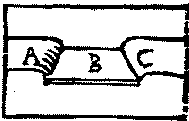
\includegraphics[max width=0.82\textwidth,max height=0.42\textheight,keepaspectratio]{images/figura10.png}\vspace{0.4em}\end{center}


\textit{Cur igitur indè non abscedit Aër, dum descendentis Aquæ }\textit{pondere è vitrea lamina truditur; sed hæret illi mordicus, nec, nisi maiori vi pulsus loco cedit? Prætereà si quis lapideam, fortè, tabulam politissimam nactus, corpus aliud graue æquè politum eidem imposuerit; posteà verò subiectam tabulam huc illuc trahat, impositum æquè corpus quò voluerit trahet; \& tamen, si pondus, quò corpus illud tabulæ innititur auferas, id huic non adhærebit. Tota igitur ratio, quæ ad tabulæ motum corpus etiam impositum moueri cogit, ex illa compressione oritur, qua graue illud tabulam subiectam premit. Iam sicuti ex eo, quòd alterum horum corporum ab altero premitur, ad eius motum hoc etiam moueri necesse est; ita assero concauum Lunæ quodammodo premi ab Aëre, siue exhalationibus inclusis si quando eas rarefieri contigerit, quod semper contingit. dum enim rarefiunt, prioris loci angustijs contemptis, ampliori extenduntur spatio, atque ambientium corporum, ac proinde Cæli ipsius, partes omnes, si qua obstent rarefactioni, quantum in ipsis est, premunt: ac proptereà mirum, si ex compressione adhæsio aliqua consequatur, quæ duo hæc corpora veluti connectat, \& colliget, ita vt ad eumdem postea motum, vtrumque moueatur.}


Continoua il Sarsi in questa sua fantasia, di voler pur, ch'io abbia detto, che l'aria non aderisca à i corpi lisci, e tersi, cosa che non si troua scritta, nè da mè, nè dal S. M. In oltre io non ben capisco, che cosa intenda egli per questa sua aderenza. S'egli intende vna copula, che resista al separarsi del tutto, e spiccarsi, l'vna dall'altra superficie, siche più non si tocchino, io dico tal aderenza esserui, ed esserui grandissima, siche la superficie, v. g. dell'acqua non si staccherà da quella d'vna falda di rame, ò di altra materia, se non con vn'immensa violenza, nè in questo caso importa se tal superficie sia, ò non sia pulita, e liscia, e basta solo vn'esquisito contatto, il qual tien tanto saldamente vniti i corpi, che forse le parti de' corpi solidi, e duri non anno altro glutine di questa, che le tenga attaccate insieme: ma questa aderenza non serue punto al bisogno del Sarsi. Ma s'egli intende vna congiunzion tale, che le due superficie, dico quella del solido, e quella dell'vmido, non possano, ne anco strisciandosi insieme mouersi l'vna contro all'altra, che sarebbe secondo il bisogno suo, dico cotale aderenza non v'essere, non solo trà vn solido, e vn liquido, ma ne anco trà due solidi; e così vederemo in due marmi ben piani, e lisci, la prima aderenza esser tanta, che alzandone vno, l'altro lo segue, ma la seconda esser così debole, che se le superficie toccantisi non saranno ben bene equidistanti all'Orizonte, ma vn sol capello inchinate; subito il marmo inferiore sdrucciolerà verso la parte inchinata, ed in somma al muouer l'vna superficie sopra l'altra non si trouerà resistenza, benche grandissima si senta nel volerle staccare, e separare. E così il toccamento dell'acqua colla barca, benche facesse grandissima resistenza à chi volesse staccare, e separar l'vna dall'altra superficie, nondimeno minima è la resistenza, che si sente nel muouersi l'vna superficie sopra l'altra fregandosi insieme, e come di sopra hò detto ancora, la Naue mossa velocissimamente non conduce seco altro, che quel velo d'acqua, che la tocca, anzi forse di questo ancora si và ella continuamente spogliando, e riuestendone altro, ed altro successiuamente, e sò che il Sarsi mi concederà, che ponendosi in Mare vna Naue bagnata con vino, ò con inchiostro, ella non auerà à pena solcate l'onde per mezo miglio, che non gli resterà più vestigio del primo licore che la circondaua; il che si può creder con gran ragione, che accaggia parimente dell'acqua che la tocca, cioè che continouamente si vada mutando, e senz'altro il seuo, con che ella si spalma, ancorche assai tenacemente vi sia attaccato, pure in breue tempo vien portato via dall'acqua, che nel suo corso le và strisciando sopra, il che non auuerrebbe se l'acqua, che tocca la Naue restasse l'istessa continouamente senza mutarsi. Quanto alla piastra di vetro, che resta à galla trà gli arginetti dell'acqua; io dico che detti arginetti non si sostengono, perche l'aderenza dell'aria colla piastra non lasci scorrer l'acqua sopra la piastra; perche se questo fusse, dourebbe seguir l'istesso, quando si ponesse nell'acqua la medesima falda alquanto vmida, chè non è credibile, che l'aria aderisca meno à vna superficie nmida, che à vna asciutta; tuttauia noi veggiamo, che quando la piastra è vmida, non si formano argini, ma subito scorre l'acqua; del sottenersi dunque detti argini altra non è la cagione, che l'aderenza dell'aria alla superficie d'essa falda, e noi veggiamo frequentissimamente gran pezzi d'acqua sostenersi in particolare sopra le foglie de i cauoli, e d'altre erbe ancora in figure colme, e rileuare in maggiore altezza assai, che quella degli arginetti, che circondano la falda notante. All'vltima proua, dou'ei vuole, che il premere, ò aggrauare, senz'altra aderenza, sia mezo bastante à far ch'vn corpo segua l'altro, com'egli essemplifica di due tauole di pietra ben liscie poste l'vna sopra l'altra, delle quali la superiore, e premente segue il moto dell'inferiore, che venga tirata verso qualche parte; io concedo l'esperienza; ma non veggo ch'ella abbia che far nel caso nostro, prima perche noi trattiamo d'vn corpo liquido, e sottile, le cui parti non anno tal connessione insieme, che al moto d'vna si debba muouere il tutto, come accade in vn corpo solido; secondariamente il Sarsi troppo languidamente proua, che 'l fuoco, l'aria, e l'essalazioni contenute dentro al concauo lunare facciano impeto, e grauino sopra la superficie d'esso concauo; mentr'egli introdduce, come causa di questa compressione, vna continoua rarefazzion d'esse sostanze, le quali dilatandosi, e perciò ricercando sempre spazij maggiori, fanno forza contro al loro contenente, e così vengono in certo modo ad attaccarsegli, siche poi seguono il mouimento suo. Languidissimo veramente è cotal discorso, perche doue il Sarsi risolutamente afferma, che le sostanze contenute si vanno continuamente rarefacendo, e dilatando, l'auuersario con non minor ragione (dico \textit{non minore}, perche il Sarsi non ne adduce niuna) dirà, ch'elle si vanno continouamente condensando, e ristringendo. Ma dato anco, ch'elle si vadano pur continouamente rarefaccendo, e che per tale rarefazzione nasca l'attaccamento al concauo, e finalmente il rapimento si può credere, che cento, e mille anni fà, quando la rarefazzione non era à gran segno al termine d'oggidì (chè così bisogna in dottrina del Sarsi), il rapimento non ci fusse, mancando la causa del farsi? anzi niuna ragione mi può ritenere ch'io non dica al Sarsi, che questa sua rarefazzione, che continouamente si và faccendo, non è ancora giunta à grado di far violenza e premer sopra il concauo della Luna, ma che ben potrebbe giungerui trà due, ò trè anni; al qual tempo io concedo, che la sfera degli elementi superiori comincerà à muouersi; ma in tanto conceda esso à mè, che sino al dì d'oggi non si sia mossa. Io non vorrei che il Sarsi, se per auuentura sentisse queste, ed altre simili risposte veramente ridicole, si mettesse à ridere, poich'egli, che ne dà occasione di proddurle tali, col lasciarsi scappar dalla mente, e poi dalla penna che alcune sostanze materiali si vadano rarefaccendo, e dilatando in perpetouo. Ma io voglio aiutare il medesimo Sarsi, ed insegnarli vn punto nella causa sua, dicendogli, che questa rarefazzione eterna, e pressione contro al concauo della Luna è superflua, tuttauolta, ch'ei possa mostrar, che l'aria vien rapita dal catino, sopra il quale ella non preme e non graua punto, essendo egli posto nella medesima region dell'aria.



\par\bigskip\noindent\phantomsection\addcontentsline{toc}{section}{§ 40}{\Large\color{rubric}\textbf{40.}}\enspace \textit{Sed videamus nunc quam verum sit experimentum illud, cui maxime Galilæi sententia innititur. Si Catinum, inquit, circa centrum, axemque suum moueatur; Aër inclusus minimè sequax, sed restitans, nulla sui parte circumagetur. Audieram iam olim à nonnullis, qui Galilæo familiariter vsi fuerant, idem illum affirmare solitum de aqua eodem catino contenta; videlicet ne illam quidem ad }\textit{vasis motum circumferri. argumento erat, quia si consistenti in eo aquæ leue aliquod corpus, \& natans, festucam scilicet aliquam, aut calamum, imposuisses superficiei catini proximum; mox cum vas ipsum circumduceretur, eodem calamus semper loco perstabat. }\textit{Ex quibus alijsque experimentis, scio aliquos ingenium Galilæi commendasse plurimùm, qui ex rebus leuissimis, atque ob oculos positis, facilitate mirabili, in rerum difficillimarum cognitionem, homines manuduceret. Neque ego in vniuersum hanc ei laudem imminutam volo. Quod autem ad rem præsentem attinet, vtrumque experimentum }(\textit{parcat mihi vera narranti Galilæus})\textit{ falsum omnino comperi. nempè ille semel, aut iterum, credo, catinum circumducebat; sic enim nullus percipitur aquæ motus: at si vlterius mouere pergat, tunc enimuerò intelliget, moueatur nè aqua ad catini motum, an verò resistat. Calamus enim, aut paleæ eidem aquæ impositæ, si non multum à catini superficie abfuerint, }\textit{citissimè circumferentur, nec, licet catinum quieuerit, illæ moueri desinent, sed aquam, cum insidentibus corporibus, ex impetu concepto, per longum tempus, tardiori tamen semper vertigine, circumagi comperies. Verùm nè quisquam incuriosè nos, ac negligenter, id expertos existimet; emisphericum vas }\textit{I. }\textit{ex orichalco affabrè orno excauatum accepimus; torno item curauimus duci axem CE. Catino ipsi iunctum; ita vt per eius centrum, in modum Sphærici axis, transiret, si produceretur. pedem autem construximus firmum, ac stabilem, ne facilè vasis motu agitaretur, atque axem per foramen E traductum, \& fulcimento, ima ex parte, innixum, perpendiculariter erectum statuimus. sic enim, manu, axe in gyrum acto, catinum etiam eodem motu ferri necesse erat. }


\begin{center}\vspace{0.4em}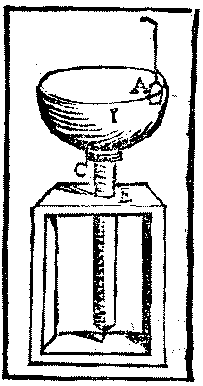
\includegraphics[max width=0.82\textwidth,max height=0.42\textheight,keepaspectratio]{images/figura11.png}\vspace{0.4em}\end{center}


\textit{Verum non aqua solum ad vasis motum fertur, sed Aër ipse, ex quo maximè exemplum desumit Galilæus. Docet id flamma candelæ, proximè, superficiei vasis admota, quæ in eamdem partem, in quam vas fertur, exigua sui corporis declinatione, deflectit. }\textit{Docet id longè clarius, serico filo tenuissimo suspensa, papyro lamella A, cuius latus alterum proximum sit interiori vasis superficiei. Si enim tunc moueatur in vnam partem catillum, in eamdem quoque sese }\textit{papyrus conuertet; \& si iterum in oppositam partem vas reciproca reuolutione voluatur, in eamdem cum adhærente Aëre etiam papyrum secum trahet. Id porrò à me non securius dici, quam verius, testes habeo nec paucos, nec vulgares: Patres primùm Romani Collegij quamplurimos, ex alijs verò, quotquot ex Magistro meo cognoscere id voluerunt, voluerunt autem multi. }\textit{Quos inter, ille mihi silendus non est, cuius non genere, magis, quam eruditione singulari clarissimum nomen sat mihi, meisque rebus luminis afferre, ac dictis facere fidem possit. Virginium Cæsarinum loquor, qui admiratus enimuerò est, rem ad hanc diem, inter multos constantissimè pro certa habitam, falsitatis vnquam argui potuisse: \& tamen vidit factum, fieri quod posse negabant plerique. Atque hæc quidem ab experientia certa sunt; quæ læuibus, fieri nunquam poterit vt vasis superficiei non adhæreant: quòd si hoc adhæsionis vinculum admittatur, motum etiam eorumdem humidorum admitti necesse est. Primùm enim pars illa, quæ vas contingit, ad vasis ductum mouebitur, quippe quæ adhæret vasi; deinde pars hæc mota aliam sibi hærentem trahet; secunda hæc tertiam: cumque motus hic fiat veluti in Spiram; non mirum, si ad vnam, aut alteram catini circumductionem, aquæ motus non percipiatur; cum primæ huius Spiralis partes valde propinquæ sint ipsi superficiei vasis; ac proinde motus, ad reliquas interiores partes, diffusus adhuc non sit; cum hæ aliquam patiantur rarefactionem, \& proptereà non illicò trahentis motum sequantur. Neque miretur quisquam, in hisce nostris experimentis exignum adeò Aëris motum esse, aquæ verò maximum. Cum enim Aër facilius, \& concrescat, \& rarescat, quam aqua; ideò quamquam ad motum vasis Aër eidem }\textit{adhærens facillimè moueatur, non tamen alium Aërem sibi proximum, eadem facilitate trahit, cum hic à reliquis Aëris consistentis partibus, maiori vi contineatur, \& exigua sui, vel concretione, vel rarefactione, vim trahentis Aëris eludere, ad breue aliquod tempus, possit. }


\begin{center}\vspace{0.4em}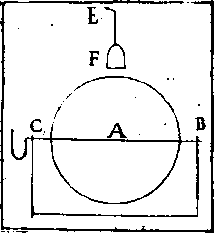
\includegraphics[max width=0.82\textwidth,max height=0.42\textheight,keepaspectratio]{images/figura12.png}\vspace{0.4em}\end{center}


\textit{Si quis tamen apertius experiri cupiat, an corpus Sphæricum in orbem actum Aërem secum trahat, hic globum A, v. g., suis innixum Polis B, \& C manubrio D circunducat, appensa charta ex E filo tenuissimo, ita vt ipsum ferè globum contingat. dum enim Sphæra in vnam rotatur partem, in eamdem charta F ab Aëre commoto fertur; si præsertim globus satis amplus fuerit, \& celerrimè circumductus. Neque tamen ex eo, quòd tum in catino, tum in Sphæra paruum adeò Aëris motum experiamur, rectè quis inferat, in concauo Lunæ, eumdem motum fore perexiguum. Ratio enim, cur in sphæra A, \& catino }\textit{I, }\textit{circumductis, non }\textit{magnus Aëris motus existat; ea inter cæteras est, quia cum catinum, \& sphæra intra Aërem posita sint tota, dum eorum motu mouendus est Aër circumfusus, semper minus est id, quod mouet, quàm quod mouetur. }


\begin{center}\vspace{0.4em}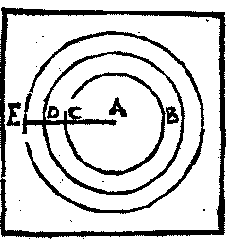
\includegraphics[max width=0.82\textwidth,max height=0.42\textheight,keepaspectratio]{images/figura13.png}\vspace{0.4em}\end{center}


\textit{Si enim, v. g., ad motum sphæræ A, superficies ipsius BC mouere debeat sibi adhærentem Aërem, circulo D, expressum; cum hic maior sit quàm circulus BC, maius à minori mouendum erit, atque idem accidet, dum circulus D trahere secum debet circulum E. At verò in concauo Lunæ, opposito planè modo se res habet; cum semper maius sit id, quod mouet, quàm quod mouetur. si enim sit Lunæ concauum circulus E, atque hic mouere debeat circulum D; D verò circulum BC; semper mouens moto maius est, \& propterea facilior motus. Hoc autem quamquam apud me nullum planè reliquerat dubitationi locum; libuit tamen modum aliquem excogitare, quo Aërem catino circumfusum, }\textit{ab eo, qui catino clauditur, separarem; sperans, haud dubium, fore vt Aër idem, qui segnius anteà ferebatur, quàm aqua, pari posteà celeritate in gyrum, ex catini circumductione, raperetur. }\textit{Quare laminam perspicuam, ne aspectum impediret, è lapide moscouito, quem vulgo, Talcum dicimus, Orificio catini amplitudine parem, quam opportunè catino ipsi posteà imponerem, paraui; in eiusdem parte media, trium ferme digitorum foramine relicto, quod tamen longè minus esse poterat. Filum deinde æreum, EF accepi, diametro catini aliquantò breuius, quod media parte }\textit{I }\textit{compressum, ac perforatum, traducto per foramen }\textit{I, }\textit{filo IG; ex G suspendi ad libræ modum, adiecique extremis EF alas duas papyraceas, mox additis, detractisque ex vtraque parte ponderibus, in æquilibrio filum æreum EF statui: ita vt fulcimentum }\textit{I }\textit{sub catini centro consisteret; alæ verò, quarta saltem digiti parte ab eiusdem superficie distarent. }


\begin{center}\vspace{0.4em}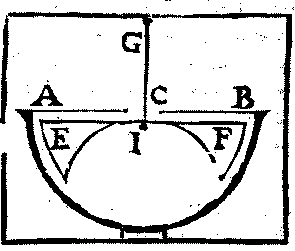
\includegraphics[max width=0.82\textwidth,max height=0.42\textheight,keepaspectratio]{images/figura14.png}\vspace{0.4em}\end{center}


\textit{Tunc vase circumacto, animaduerti, post alteram euolutionem, alas, ac libram totam in gyrum moueri, \& primò quidem lentè, deinde citatiori motu, qui tamen nondum motum aquæ æquabat: Quare superimposui laminam AB perspicuam, quam paraueram, ita vt Aër catino contentus à reliquo separaretur, vel solo foramine C eidem necteretur. Tunc enimuerò, ad vasis motum, ferri citius visa est libra F, ac breui celeriter adeò agi cœpit, vt catini ipsius motum, quamuis velocissimum, assequeretur. vt hinc videas, quotiescumque mouens moto maius fuerit, tunc longè faciliorem motum futurum: imposito enim vasi operculo AB, tunc superficies interior catini, \& operculi simul, ad cuius motum mouendus est Aër, maior est Aëre proximè mouendo; est enim superficies illa continens; Aër verò contentus.}


\begin{center}\vspace{0.4em}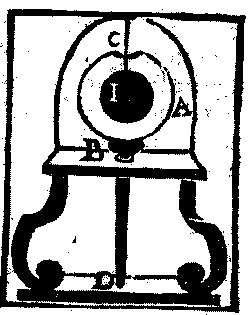
\includegraphics[max width=0.82\textwidth,max height=0.42\textheight,keepaspectratio]{images/figura15.png}\vspace{0.4em}\end{center}


\textit{Idem denique expertus sum, euentu pari, in Sphæra vitrea A, quantum fieri potuit, exactissima summa tantum parte C, perforata ad laminam }\textit{I, }\textit{inducendam. Eadem enim Sphæra axi BD, imposita, axeque ipso circumacto, non Sphæra solum A, sed \& lamina }\textit{I }\textit{suspensa, quamuis multùm ab interiore superficie Sphæræ distaret, celerrimè moueri visa est.  }\textit{Atque ita nulli, aut industriæ, aut labori parcendum duxi, vt quamplurimis idem experimentis, quam diligentissimè comprobarem. }\textit{Hæc porrò postrema experimenta videre ijdem illi, qui superius à me commemorati sunt; vt necesse non habeam, eosdem iterum testari. Illud etiam adnotandum duxi, æstiuo nos tempore }\textit{hæc omnia expertos fuisse, quo, vt calidior, ita siccior Aër existit, magisque proinde ad Ignis naturam accedit; quem omnium elementorum minimè aptum adhæsioni existimat Galilæus. Ex quibus omnibus illud saltem colligere licet, tum ad catini motum, \& Aërem, \& Aquam }\textit{moueri, tum læuibus etiam corporibus Aërem adhærescere atque ad eorum motum agi, quæ constanter adeò pernegauit Galilæus.}


Entra ora il Sarsi nel copiosissimo apparato d'esperienze per confermare il suo detto, e riprouare il nostro, le quali, perche furon fatte alla presenza di V. S. Illustriss. io me ne rimetto à lei, come quello, che più tosto deuo aspettarne il suo giudicio che interporui il mio; però se le piacerà, potrà rilegger quel, che resta sino alla fine della proposizione; dou'io le anderò solamente toccando alcuni particolari sopra varie cosette così alla spezzata. E prima, questo, che il Sarsi cerca d'attribuirmi nel primo ingresso delle sue esperienze, è falsissimo, cioè ch'io abbia detto, che l'acqua contenuta nel catino resti non men, che l'aria immobile al mouimento in giro di esso vaso; non però mi merauiglio che l'abbia scritto, perche ad vno, che continouamente và riferendo in sensi contrari le cose scritte, e stampate da altri, si può bene ammettere, ch'egli alteri quelle ch'ei dice d'auer solamente sentite dire; ma non mi par già che resti del tutto dentro a' termini della buona creanza il pubblicar colle stampe ciò, ch'altri sente dire del prossimo, e tanto più quando, ò per non l'auere inteso bene, ò pur di propria elezzione ei si rapporta molto diuerso da quello, che fù detto, come di presente accade di questo. Tocca à mè S. Sarsi, e non à voi, ò ad altri lo stampar le cose mie, e farle pubbliche al Mondo, e perche quando (come pur talora accade) alcuno nel corso del ragionar dicesse qualche vanità, deue esser chi subito la registri, e stampi, priuandolo del beneficio del tempo, e del poterui pensar sopra meglio, e da per se stesso emendare il suo errore, e mutare opinione, ed in somma fare à suo talento del suo ceruello, e della sua penna? Quello che può auer sentito dire il Sarsi, ma, per quanto veggo, non ben capito, è certa esperienza ch'io mostrai ad alcuni letterati costì in Roma, e forse fu in camera di V. S. Illustriss. stessa, parte in dichiarazione, e parte in confutazione d'vn terzo moto attribuito dal Copernico alla Terra. Pareua à molti cosa molto improbabile e che perturbasse tutto il sistema Copernicano, il terzo moto annuo, ch'egli assegna al globo terrestre intorno al proprio centro al contrario di tutti gli altri mouimenti celesti, i quali col figurarsi fatti tutti, tanto quelli delli eccentrici, quanto quelli delli epicicli, ed il diurno, e l'annuo d'essa Terra nell'orbe magno, da Ponente verso Leuante, questo solo douesse nell'istessa Terra esser fatto da Oriente verso Occidente, contro agli altri due propri, e contro agli altri tutti di tutti i Pianeti; io soleuo leuar questa difficoltà col mostrare, che tal'accidente non solo non era improbabile, ma conforme alla Natura, e quasi necessario; e che qualsiuoglia corpo collocato è sostenuto liberamente in vn mezo tenue, e liquido, se sarà portato per la circonferenza di vn gran cerchio, acquisterà spontaneamente vna conuersione in sè medesimo, al contrario dell'altro gran mouimento, il qual effetto si vedeua pigliando noi in mano vn vaso pien di acqua e mettendo in esso vna palla notante perche stendendo noi il braccio, e girando sopra i nostri piedi, subito veggiamo la detta palla girare in sè stessa al contrario e finir la sua conuersione nell'istesso tempo, che noi finiamo la nostra. Onde cessar doueua la merauiglia, anzi merauigliarsi, quando altrimenti accadesse, se essendo la Terra vn corpo pensile, e sospeso in vn mezo liquido, e sottile, ed in esso portata per la circonferenza d'vn gran cerchio nello spazio d'vn anno, ella non auesse di sua natura, e liberamente acquistata vna conuersione parimente annua in sè medesima al contrario dell'altra. E tanto diceuo per rimuouer l'improbabilità attribuita al sistema del Copernico, al che soggiungeuo poi, che chi meglio consideraua, conosceua, che falsamente veniua da esso Copernico attribuito vn terzo moto alla Terra, il quale non è altramente vn muouersi, ma vn non si muouere ed vna quiete; perch'è ben vero, che à quello che tiene il vaso apparisce muouersi, e rispetto a sè, e rispetto al vaso, e girare in sè stessa la palla posta in acqua, ma la medesima palla paragonata colle mura della stanza, e colle cose esterne, non gira altrimenti, nè muta inchinazione, ma qualunque suo punto che da principio riguardaua verso vn termine esterno segnato nel muro, ò in altro luogo più lontano, sempre riguarda verso lo stesso. E questo è quanto da mè fu detto; cosa, come V. S. Illustriss. vede, molto diuersa dalla riferita dal Sarsi. Questa esperienza, e forse qualch'altra, potè dare occasione à chi più volte si trouò presente a' nostri discorsi di dir di mè quello, che in questo luogo riferisce il Sarsi, cioè che per certo mio natural talento soleuo alcuna volta con cose minime, facili, e patenti, esplicarne altre assai difficili, e recondite; la qual lode il Sarsi non mi nega in tutto, ma come si vede in parte m'ammette: la qual concessione io deuo riconoscere dalla sua cortesia, più che da vna interna, e verace concessione, perche, per quanto io posso comprendere, egli non è di quelli, che così di leggiero si lascino persuadere dalle mie facilità, poich'egli stesso riputando che la scrittura del S. M. sia mia cosa, dice nel fine del precedente essame, quella esser stata scritta con parole molto oscure, e tali, ch'egli non hà potuto indouinare il senso. Già, come hò detto, quanto all'esperienze, me ne rimetto a V. S. Illustriss. che le hà vedute, e solo incontro à tutte ne replicherò vna scritta di già dal S. M. nella sua lettera, dopò che auerò fatto vn poco di considerazione sopra certa ragione, che il Sarsi accoppia coll'esperienze la qual ragione io veramente pagherei gran cosa, che fusse stata taciuta per riputation sua, e del suo Maestro ancora, quando vero fusse, ch'egli fusse discepolo di chi egli si fà. Oimè, Sig. Sarsi, e quali essorbitanze scriuete voi? Se non v'è qualche grand'error di stampa, le vostre parole son queste: \textit{Hinc videas, quotiescunque mouens moto maius fuerit, tunc longe faciliorem motum futurum imposito enim vasi operculo AB. tunc superficies interior catini, \& operculi simul, ad cuius motum mouendus est Aër proximè mouendo: est enim superficies illa continens, Aër verò contentus}. Or rispondetemi in grazia, S. Sarsi: questa superficie del catino, e del suo coperchio, con chi la paragonate voi, colla superficie dell'aria contenuta, ò pur coll'istessa aria, cioè col corpo æreo? Se colla superficie è falso, che quella sia maggior di questa, anzi pur sono elleno egualissime, che così v'insegnerà l'assioma Euclidiano, cioè che \textit{Quæ mutuo congruunt, sunt æqualia}; ma se voi intendete di paragonar la superficie contenente coll'istessa aria, come veramente suonan le vostre parole, fate due errori troppo smisurati; prima col paragonare insieme due quantità di diuersi generi, e però incomparabili, chè così vuole vna diffinizion d'Euclide. \textit{Ratio est duarum magnitudinum eiusdem generis}; e non sapete voi, che chi dice questa superficie è maggior di quel corpo, erra non men di quel, che dicesse la settimana è maggior d'vna Torre, ò l'oro è più graue della nota Cefautte? l'altro errore è, che quando mai si potesse far paragone trà vna superficie, ed vn solido, il negozio sarebbe tutto all'opposito di quello, che scriuete voi, perche non la superficie sarebbe maggior del solido, ma il solido più di cento milioni di volte maggior di lei. S. Sarsi, non vi lasciate persuadere simili chimere, nè anco la general proposizione, che 'l contenente sia maggior del contenuto, quando bene ambedue si prendessero di quantità comparabili frà di loro; altrimenti bisognerà, che voi crediate, che d'vna balla di lana, il guscio, ò inuoglio sia maggior della lana, che vi è dentro, perche questa è contenuta, e quello è il contenente: e perche sono della medesima materia bisognerà anco, che il sacco pesi più essendo maggiore. Io fortemente dubito, che voi abbiate preso con qualche equiuocazione vn pronunciato, che è verissimo, quando vien preso al suo diritto senso, il qual'è, che il contenente è maggior del contenuto, tutta volta che per contenente si prenda il contenente col contenuto insieme, e così vn quadrato descritto intorno à vn cerchio è maggior di esso cerchio, pigliando tutto il quadrato; ma se voi vorrete prender solo quello, che auanza del quadrato, detrattone il cerchio, questo non è altrimenti maggiore, ma minore assai d'esso cerchio, ancorch'ei lo circondi, e racchiuda. Aime, e non m'accorgo del fuggir dell'ore? e vò logorando il mio tempo intorno a queste puerizie? orsù, contro à tutte l'esperienze del Sarsi, potrà V. S. Illustriss. fare accommodare il catino conuertibile sopra il suo asse; e per certificarsi quello, che segua dell'aria contenutaui dentro, mentre quello velocemente và in giro, pigli due candelette accese, ed vna n'attacchi dentro all'istesso vaso vn dito, ò due lontana dalla superficie, e l'altra ritenga in mano, pur dentro al vaso, in simil lontananza dalla medesima superficie, faccia poi con velocità girar il vaso, che se in alcun tempo l'aria anderà parimente con quello in volta, senza alcun dubbio, mouendosi il vaso l'aria contenuta, e la candeletta attaccata tutto colla medesima velocità, la fiammella, d'essa candela non si piegherà punto, ma resterà, come se il tutto fusse ferma (che così à punto auuiene, quando vn corre con vna lanterna entroui racchiuso vn lume acceso, il quale non si spegne, nè pur si piega, auuenga che l'aria ambiente và con la medesima prestezza, il qual effetto anco più apertamente si vede nella Naue, che velocissimamente camini, nella quale i lumi posti sotto couerta non fanno mouimento alcuno, ma restano nel medesimo stato, che quando il Nauilio stà fermo); ma l'altra candeletta ferma darà segno della circolazion dell'aria, che ferendo in lei la farà piegare. Ma se l'euento sarà al contrario, cioè se l'aria non seguirà il moto del vaso, la candela ferma manterrà la sua fiammella diritta, e quieta, e l'altra portata dall'impeto del vaso vrtando nell'aria quieta si piegherà; ora, nell'esperienze vedute da mè, è accaduto sempre, che la fiammella ferma è restata accesa, e diritta, ma l'altra, attaccata al vaso, si è sempre grandissimamente piegata, e molte volte spenta; ed il medesimo di sicuro vederà anco V. S. Illustriss. ed ogn'altro, che voglia farne proua. Giudichi ora quello che si deue dire che faccia l'aria. Dall'esperienze del Sarsi il più che se ne possa cauare, è ch'vna sottilissima falda d'aria alla grossezza di vn quarto di dito contigua alla concauità del vaso venga portata in giro, e questa basta à mostrar tutti gli effetti scritti da lui; e di questo ne può esser bastante cagione l'asprezza della superficie, ò qualche poco di cauità, ò prominenza più in vn luogo, ch'in vn altro. Ma finalmente quando il concauo della Luna portasse seco vn dito di profondità dell'essalazioni contenute, che ne vuol fare il Sarsi? e non creda che se il catino ne porta, v. g., vn mezo dito, che vn vaso maggiore ne abbia a portar più, perche io credo più tosto, ch'ei ne porterebbe manco, e così anco non credo, che la somma velocità colla quale detto concauo lunare passa tutto il cerchio, diciamo in 24. ore, abbia à far più assai; anzi io mi voglio prendere ardir di dire, che mi par quasi vedere per nebbia, ch'ei non farebbe più, ma più tosto manco di quello, che si faccia vn catino che pure in ore 24. desse vna riuoluzione sola; ma pongasi pure, e concedasi al Sarsi, che 'l concauo lunare rapisca, quanto si è detto dell'essalazion contenuta, che sarà poi? e che ne seguirà in disfauor della principal causa, che tratta il S. M. sarà forse vero, che per questo moto si abbia ad accender la materia della cometa? ò pur sarà vero, ch'ella non si accenderà, nè mouendosi, nè non si mouendo? così cred'io: perche se il tutto stà fermo, non s'ecciterà l'incendio, per lo quale Arist. ricerca il moto. Ma se il tutto si muoue, non vi sarà l'attrizione, e lo stropicciamento, senza il quale non si desta il calore, non che l'incendio. Or'ecco, e dal Sarsi, e da mè fatto vn gran dispendio di parole in cercar se la solida concauita dell'orbe lunare, che non è al Mondo, mouendosi in giro, la qual già mai non s'è mossa, rapisce seco l'elemento del fuoco, che non sappiamo se vi sia, e per esso l'essalazioni, le quali perciò s'accendano, e dien fuoco alla materia della cometa, che non sappiamo se sia in quel luogo, e siamo certi; che non è robba ch'abbruci. E quì mi fà il Sarsi souuenire del detto di quell'argutissimo Poeta. Per la spada d'Orlando, che non anno, e forse non son anco per auere, queste mazzate da ciechi si danno. Ma è tempo, che vegniamo alla seconda proposizione, anzi pure prima, che vi passiamo, già che il Sarsi replica nel fine di questa, ch'io abbia constantemente negato, che l'acqua si muoua al moto del vaso, e che l'aria, e gli altri corpi tenui aderiscano a' corpi lisci, replichiamo noi ancora, ch'ei non dice la verità, perche mai, nè il S. M. ned io abbiamo detta, ò scritta alcuna di queste cose, ma bene il Sarsi, non trouando doue attaccarsi, si và fabbricando gli vncini da per sè stesso.



\par\bigskip\noindent\phantomsection\addcontentsline{toc}{section}{§ 41}{\Large\color{rubric}\textbf{41.}}\enspace Passi ora V. S. Illustriss. Alla seconda proposizione. \textit{Ait Aristoteles motum causam esse caloris, quam propositionem omnes ita explicant; non quasi motui tribuendus sit calor, vt effectus proprius, \& per se }(\textit{hic enim est acquisitio loci})\textit{ sed quia, cum per localem motum corpora atterantur; ex attritione autem calor excitetur; mediatè saltem, motus caloris causa dicitur; neque est, quòd hac in re Aristotelem reprehendat Galilæus, cum nihil ipse adhuc afferat ab eiusdem dictis, alienum. Dum verò ait præterea, non quamcumque attritionem satis esse ad calorem producendum, sed illud etiam potissimum requiri, vt partes attritorum corporum aliquæ per attritionem deperdantur, hìc planè totus suus est, nec quicquam ab alio mutuatur. Cur autem hæc partium consumptio ad calorem producendum, requiritur? An quòd ad eumdem calorem concipiendum, rarescere corpora necesse sit; in omni verò rarefactione comminui eadem corpora videantur, ac minutissimæ quæque particulæ e}\textit{uolent? At rarefieri corpora possunt, nulla facta partium separatione, ac proinde, neque consumptione. An ideò hæc comminutio requiritur, vt prius particulæ illæ, vtpotè calori concipiendo }\textit{magis aptæ, calefiant, hæ verò postea, reliquo corpori calorem tribuant? Nequaquam. licet enim particulæ illæ, quò minutiores fuerint, magis calori concipiendo aptæ sint: ex quo fit, vt sæpè ex attritione ferri, excussus puluisculus in ignem abeat: illæ tamen, cum statim euolent aut decidant, non poterunt reliquo corpori, cui non adhærent, calorem tribuere.}


Vuole il Sarsi nel primo ingresso di questa disputa concordare il S. M. ed Arist. e mostrar, che ambedue an pronunziato l'istessa conchiusione, mentre l'vno dice, che'l moto è causa di calore, e l'altro, che non il moto, ma lo stropicciamento gagliardo di due corpi duri. E perche la proposizione del S. M. è vera, nè ha bisogno di chiose, il Sarsi interpreta l'altra con dire, che se bene il moto, come moto non è cagione del caldo, ma l'attrizione, nulladimeno, non si facendo tale attrizione senza moto possiamo dire che almanco secondariamente il moto sia causa. Ma se tale fù la sua intenzione, perche non disse Aristotile l'attrizione? io non sò vedere perche potendo vno dir bene assolutamente con vna semplicissima, e proprijssima parola, ei debba seruirsi d'vna impropria, e bisognosa di limitazioni, ed in somma d'esser finalmente trasportata in vn'altra molto diuersa. In oltre posto, che tale fusse il senso d'Aristotile, egli però è differente da quello del S. M. perche ad Aristotile basta qualunque confricazione di corpi, benche tenui, e sottili, e fino dell'aria stessa; ma il S. M. ricerca due corpi solidi, e stima, che il volere assottigliare, e tritar l'aria sia maggior perdimento di tempo, che quello di chi vuole (com'è in prouerbio) pestar l'acqua nel mortaio. Io non son fuor d'opinione, che possa esser, che la proposizione sia verissima, presa anco nel semplicissimo senso delle parole, e forse potrebbe esser, ch'ella vscisse da qualche buona scuola antica, ma che Aristotile non auendo ben penetrata la mente di quegli antichi, che la profferirono, ne træsse poi vn sentimento falso, forse non è questa sola proposizione vera in sè stessa, ma appresa in sentimento non vero nella Filosofia Peripatetica; ma di questo ne toccherò qualche cosa più à basso. Ora seguitiamo il Sarsi, il quale vuole contro al detto del S. M. che senza verun consumamento de' corpi, che si stropicciano, sin che si riscaldino, si possa eccitare il calore; il che và prouando prima con discorso, poi con esperienze. Ma quanto al discorso io posso sbrigarmi in vna parola sola da tutte le sue instanze, poiche, faccendo egli alcune interrogazioni al S. M. egli stesso risponde per quello, e poi confuta le risposte; talche se io dirò, che il S. M. non risponderà in quella guisa, bisogna, che il Sarsi si quieti. E veramente, quanto alla prima risposta io non credo, che il S. M. dicesse, che per riscaldarsi bisogni prima, che i corpi si rarefacciano, e che rarefaccendosi si sminuzzolino, e che le parti più sottili volino via come scriue il Sarsi; dalla qual risposta mi par di comprendere, ch'ei discordi dalla mente del S. M. e che conuenendo in questa azzione considerare il corpo, che hà da produrre il calore, e quello, che l'hà da riceuere, il Sarsi stimi, che il S. M. ricerchi la diminuzione, e consumamento di parti nel corpo, che hà da riceuere il calore, ma io credo ch'ei voglia, che quello, che l'hà da produrre sia quello, che si diminuisce; siche in somma non il riceuere, ma il conferir calore sia quel che fà la diminuzione nel conferente. Come poi si possano rarefare i corpi senza alcuna separazion di parti, e come cammini questo negozio della rarefazzione, e condensazione, del quale mi par, che con molta confidenza parli il Sarsi l'auerei ben volentieri veduto più distintamente dichiarato essendo, appresso di mè vna delle più recondite, e difficili questioni della Natura. E manifesto ancora, che il S. M. non auerebbe data la seconda risposta, cioè che tal consumamento di parti sia necessario, acciochè prima si riscaldino queste parti più minute, come più atte per la lor sottigliezza à riscaldarsi, e da esse poi venga riscaldato il resto del corpo, perche così la diminuzione toccherebbe pure al corpo, che hà da esser riscaldato, ed il S. M. la dà à quello, che hà da riscaldare, deuesi però auuertire, che bene spesso accade essere vno istesso corpo quello, che prodduce il calore, e quello che lo riceue, e così martellandosi sopra vn chiodo le parti sue nel soffregarsi violentemente eccitano il calore, e l'istesso chiodo è quello, che si riscalda, ma quello, che hò voluto sin quì dire, è che il consumamento di parti dipende dall'atto del proddurre il calore, e non da quello del riceuerlo, come per auuentura più distintamente mi dichiarerò più di sotto. In tanto sentiamo l'esperienze onde il Sarsi pensa d'auer palesato potersi con l'attrizione proddur senza consumamento alcuno.



\par\bigskip\noindent\phantomsection\addcontentsline{toc}{section}{§ 42}{\Large\color{rubric}\textbf{42.}}\enspace \textit{Sed quando ab experientia exempla petere libet. quid si, nulla partium deperditione, ex motu, corpus aliquod calefiat? Ego certè cum æris frustulum, omni prius extersa rubigine, ac situ, ne quis fortè puluisculus adhæreret, ad Argentarij libram perexiguam, exactissimamque, ponderibus minutissimis, expendissem }(\textit{cum etiam quingentesimas duodecimas vnius vnciæ partes haberem})\textit{ ac pondus diligentissimè obseruassem; validissimis mallei ictibus æs idem in laminam extendi: id verò inter ictus, \& mallei verrerba, bis, terquè adeò incaluit, vt manibus attrectari non posset. Cum igitur iam toties incaluisset; experiri libuit }\textit{eadem libra, ijsdemque ponderibus, num aliquod ponderis dispendium, iacturamque passum fuisset; \& tamen ijsdem planè momentis constare comperi; incaluit igitur per attritionem æs illud, nullo partium suarum detrimento, quod Galilæus negat.}\textsc{ }\textit{Audieram etiam aliquid simile librorum compactoribus euenire, cum plicatas illas chartarum moles malleo diutissimè, ac validissimè tundunt: expertus enim est illorum non nemo, eodem postea illas fuisse pondere, quo fuerant prius; incalescere tamen easdem inter ictus maximè, ac penè comburi. Quòd si quis fortè hoc loco asserat deperdi quidem partes, sed adeò minutas, vt sub libra, quamuis exigua, examen non cadant. quæram ego ex illo, vnde norit partes esse deperditas. neque enim video, quonam alio id modo aptius, ac diligentius inquiram.}\textit{ }\textit{Deinde verò; si adeò exigua est hæc partium iactura, vt sensu percipi nequeat, cur tantum caloris excitauit? Præterea dum ferrum lima expolitur, calefit quidem, minus tamen, aut certè non plus, quàm cum malleo validissimè tunditur; \& tamen maior longè partium deperditio ex limatura, quàm ex contusione, existit.}


Che il Sarsi con isquisita bilancia non abbia ritrouato diminuzion di peso in vn pezzetto di rame battuto, e riscaldato più volte; gliel voglio credere; ma non già che per questo egli non si sia diminuito, essendo che può benissimo accadere quello esser diminuito tanto poco, che a qualsiuoglia bilancia resti cosa impercettibile. E prima io domando al Sarsi, se pesato vn bottone d'argento, e poi doratolo, e tornato à pesarlo, ei crede che l'accrescimento fusse notabile, e sensibile. Bisogna dir di nò, perche noi veggiamo l'oro indursi à tanta sottigliezza, che anco nell'aria quietissima si trattiene, e lentissimamente cala à basso; e con tali foglie può dorarsi alcun metallo, in oltre questo medesimo bottone verrà adoperato due, ò trè mesi auanti, che la doratura sia consumata, ò pur consumandosi finalmente, chiara cosa è, che ogni giorno, anzi ogn'ora, s'andaua diminuendo. Di più pigli vna palla d'ambra, muschio, ed altre materie odorate, io dico, che portandola addosso alcuno quindici giorni, empirà d'odore mille stanze, e mille strade, ed in somma ogni luogo, dou'egli capiterà, nè questo si farà senza diminuzione di quella materia, senza la quale indubitatamente non anderà l'odore, pure, tornandosi in capo à tal tempo à ripesarla, non si trouerà sensibil diminuzione. Ecco dunque trouate al Sarsi diminuzioni insensibili di peso, fatte per lo consumamento di mesi continoui, ch'è altro tempo, che vn'ottauo d'ora, che douette durare il suo martellare sopra il pezzetto di rame. E tanto è più esquisita, vna bilancia da saggiatori, ch'vna stadera filosofica. Aggiungendo di più, che può molto bene essere, che la materia, che attenuata produce il caldo sia ancora assai più sottile della sostanza odorifera attento, che questa si racchiude in vetri, e metalli, per li quali essa non traspira, ma non già quella del calore, che trapassa per tutti i corpi. Ma quì muoue il Sarsi vn'instanza, e dice, se il cimento della bilancia non basta à mostrarci vn così piccolo consumamento, come potete voi auerlo conosciuto? l'obiezzione è assai ingegnosa, ma non però tanto, ch'vn poco di Logica naturale non auesse auuto à mostrarne la soluzione. Ed eccone il progresso de i corpi, S. Sarsi, che si stropicciano insieme, alcuni sono, che assolutamente, e sicuramente non si consumano punto, altri, che grandemente, e molto sensibilmente si consumano, ed altri che si consumano bene, ma insensibilmente. Di quelli che stropicciandosi non si consumano punto, quali sarebbon due specchi benissimo lisci, il senso ci mostra, che non si riscaldano; di quelli che si consumano notabilmente, come vn ferro nel limarsi, siamo sicuri che si riscaldano. Adunque di quelli che noi siamo dubbi, se nel fregarsi si consumino, ò nò, se troueremo pel senso, che si riscaldino, dobbiamo dire, e credere, che si consumino ancora, e solo si potrà dire, che non si consumino quelli, che ne anco si riscaldano. A quanto sin quì hò detto, voglio prima, ch'io vada più auanti, aggiungere per ammæstramento del Sarsi, come il dire questo corpo alla bilancia non è calato di peso, adunque di lui non si è consumata parte alcuna, è discorso assai fallace, potendo esser, che se ne sia consumato, e che il peso non solo non sia diminuito, ma anco tal volta cresciuto; il che accaderà sempre, che quello che si consuma, e rimuoue, sia men graue in specie del mezo nel quale si pesa; e così per essempio può accadere, ch'vn pezzo di legno, per auere in sè molti nodi; e per esser vicino alle radici, messo nell'acqua cali al fondo, e v. g., vi pesi quattr'once, e che limandone via, non del nocchioruto, nè della radice, ma della parte più rara, e che per sè stessa è men graue in ispecie dell'acqua, siche in parte sosteneua tutta la mole, può esser dico, che il rimanente pesi più, che prima nel medesimo mezo; e così parimente può essere, che nel limarsi, ò nel fregarsi insieme due ferri, ò due sassi, ò due legni, si separi da loro qualche particella di materia men graue dell'aria, la quale quando sola si rimouesse, lascerebbe quel corpo più graue, che prima. E che quanto io dico sia detto con qualche probabilità, e non per una semplice fuga e ritirata, lasciando la fatica all'auuersario di riprouarla, faccia V. S. Illustriss. diligente osseruazione nel romper vetri. ò pietre, ò qualunque altre materie; che ella in ciascheduno spezzamento, ne vederà vscire vn fumo manifestissimamente apparente, il quale per aria se ne ascende in alto, argomento necessario dell'essere egli più leggieri di lei. Questo osseruai io prima nel vetro, mentre con vna chiaue, ò altro ferro l'andauo scantonando, e tondando, doue, oltre à i molti pezzetti, che saltano via in diuerse grandezze, ma tutti cascano in terra, si vede vn fumo sottile ascendente sempre; ed il medesimo si vede accadere nel frangere in simil modo qualsiuoglia pietra; e di più oltre à quello, che ci manifesta la vista, l'odorato ci dà argomento ed indizio molto chiaro, che per auuentura si partono oltre al detto fumo, altre parti più sottili, e perciò inuisibili, sulfuree e bituminose, le quali per tale odore, che ci arrecano si fanno manifeste. Or vegga il Sarsi, quanto il suo filosofare è superficiale, e poco si profonda oltre alla scorza. Nè si persuada di poter venir con risposte di limitazioni, di distinzioni, di \textit{per accidens}, di \textit{per se}, di \textit{mediatè}, di primario, di secondario, ò d'altre chiacchiere, ch'io l'assicuro, che in vece di sostenere vn'errore, ne commetterà cento più graui, e produrrà in campo sempre vanità maggiori, maggiori dico anco di questa, che mi resta da considerare nel fin della presente particola; dou'egli prima si merauiglia, come possa esser, che sendo quel che si consuma cosa impercettibile alla bilancia, possa nondimeno proddur tanto calore, dapoi soggiunge, che d'vn ferro, che si lima, gran parte se ne consuma e assaissimo maggiore, che quando ei si batte col martello; nulladimeno, non più si scalda limando, che battendolo. Vanissimo è questo discorso, mentre altri vuole col peso misurare la quantità di cosa, che non hà peso alcuno, anzi è leggierissima, e nell'aria velocemente sormonta; e quando pure quello, che si conuerte in materia calda, mentre si fà vna gagliarda confricazione, fusse parte dell'istesso corpo solido, non douerà alcuno marauigliarsi, che piccolissima quantità di quello possa rarefarsi, ed istendersi in ispazio grandissimo, s'ei considererà in quanta gran mole di materia ardente, e calda si risolue vn piccol legno, della quale la fiamma visibile, è la minor parte, restando di gran lunga maggiore l'insensibile alla vista, ma ben sensibile al tatto. Quanto poi all'altro punto auerebbe qualche apparenza l'instanza, se il S. M. auesse mai detto, che tutto quel ferro, che si consuma limando, douentasse materia calorifica, perche così parrebbe ragioneuol cosa, che molto più scaldasse il ferro consumato colla lima, che il percosso col martello, ma non è la limatura quella, che scalda, ma altra sostanza incomparabilmente più sottile.



\par\bigskip\noindent\phantomsection\addcontentsline{toc}{section}{§ 43}{\Large\color{rubric}\textbf{43.}}\enspace Ma seguitiamo innanzi. \textit{Ego igitur multum conferre arbitror ad maiorem, minoremue calefactionem corporum attritorum, qualitates eorumdem; sint ne videlicet illa calidiora an frigidiora, remque hanc ex multis alijs pendere, de quibus statuere adeò facilè non sit. Nam si Ferulas duas, corpora leuissima, ac rarissima, mutua, aut alterius ligni confricatione attriueris, ignem breui concipient: non idem in lignis alijs accidit, durioribus, ac densioribus, quamuis eadem diutius, ac vehementius atteri consumique contingat. }\textit{Seneca certè, facilius inquit, attritu calidorum ignis existit; ex quo fieri ait, vt æstate plurima fiant fulmina, quia plurimum calidi est. Præterea ferreus puluis in flammam coniectus exardescit, non verò quicumque alius puluis e marmore. Quare si Aëre plurimum exalationum calidarum fuerit, eumdemque ex vehementi aliquo motu atteri }\textit{contigerit, non video, cur calefieri, atque etiam incendi non possit. Tunc enim, cum rarus sit, ac siccus, multumque admixtum calidi habeat, ad ignem concipiendum aptissimus est.}


Quì doue pare, che il Sarsi si apparecchi per produrre con dottrina più salda migliore esplicazione delle difficoltà, che si trattano, non veggo, ne che venga apportato molto di nuouo, nè di gran pregiudicio alle cose del S. M. Imperocchè il dire, che molto conferisce al maggiore, ò minor riscaldamento de' corpi, che si stropicciano insieme, l'essere essi di qualità calda, ò fredda, e che anco da molte altre cose, non così ben manifeste dipende questo negozio, lo credo io pur troppo, ma non mi par già di farci acquisto veruno, per esser di questo, che mi vien detto, la seconda parte troppo recondita, e la prima troppo manifesta, e notoria; atteso, che in sostanza non mi dice altro, se non che più si scaldano quei corpi, che son più caldi, ò più disposti allo scaldarsi, e meno quelli, che son più freddi; così parimente quello, che segue appresso, che per la confricazione alcuni legni, cioè i più leggieri, e rari, s'accendano più facilmente, che altri più duri, e densi, ancorche questi più gagliardamente e più lungo tempo s'arruotino insieme lo credo parimente, ma ciò non veggo, che faccia contro al S. M., che mai non hà detto in contrario; e non è adesso, ch'io sapeuo, che più presto s'infiammaua vn pennecchio di stoppa in vn fuoco, benche lentissimo, che vn pezzo di ferro nella fucina ben'ardente. A quello, ch'ei soggiunge, e fortifica col testimonio di Seneca, cioè che la State sia per aria maggior copia d'essalazioni secche, e che perciò si facciano molti fulmini, io ci presto l'assenso; ma dubito bene circa'l modo dell'accendersi cotali essalazioni insieme coll'aria, e se ciò auuenga per l'attrizione cagionata per alcun mouimento. Io riputerei vero, quanto viene scritto dal Sarsi, se prima egli m'auesse accertato non essere in Natura altri modi di suscitar l'incendio fuori, che questi due, cioè, ò col toccar la materia combustibile con vn fuoco già attualmente ardente, come quando con vn moccolo acceso s'accende vna torcia; ouero con l'attrizion di due corpi non ardenti; ma perche altri modi ci sono, come per la riflessione de' raggi solari in vno specchio concauo, ò per la refrazzion de' medesimi in vna palla di cristallo, ò d'acqua, ed anco s'è veduto taluolta infiammarsi per le strade mediante l'eccessiuo caldo, le paglie, ed altri corpi sottili, e questo farsi senza alcuna commozione, ò agitazione, anzi solamente quando l'aria è quietissima, e che per auuentura, s'ella fusse agitata, e spirasse vento, l'incendio non ne seguirebbe; perche dico ci sono questi altri modi, perche non poss'io stimar, che ve ne possa esser qualche altro diuerso da questi? per lo quale l'essalazioni per aria, e trà le nubi si accendano? e perche debbo io attribuire ciò ad vn vehemente mouimento, se io veggo prima, che senza l'arrotamento de' corpi solidi, quali non si trouano trà le nuuole, non si suscita l'incendio, ed oltre à ciò niuna commozione si scorge in aria, ò nelle nuuole, quando è maggior la frequenza de' lampi, e de' fulmini, io stimo, che il dir questo non abbia in se più di verità, che quando i medesimi Filosofi atrribuiscono il gran romor de' tuoni allo stracciamento delle nuuole, ò all'vrtarsi insieme l'vna contro l'altra; tuttauia nello splendor de' maggiori baleni, e quando si prodduce il tuono, non si scorge nelle nuuole pure vn minimo mouimento, ò mutazion di figura, il quale ad vn tanto squarciamento douerebbe esser grandissimo. Lascio stare, che i medesimi Filosofi, quando tratteranno poi del suono, vorranno nella sua produzzione la percussione de' corpi duri, e diranno, che perciò la lana, nè la stoppa, nel percuotersi non fanno strepito; ma poi quando n'aueranno bisogno, la nebbia, e le nuuole percuotendosi renderanno il massimo di tutti i rumori. Trattabile, e benigna Filosofia, che così piacevolmente, e con tanta ageuolezza si accommoda alle nostre voglie, ed alle nostre necessità!



\par\bigskip\noindent\phantomsection\addcontentsline{toc}{section}{§ 44}{\Large\color{rubric}\textbf{44.}}\enspace Or passiamo auanti à essaminar l'esperienze della freccia tirata coll'arco, e della palla di piombo tirata colle scaglie infocate, e strutte per aria, confermate coll'autorità d'Aristotile, di molti gran Poeti, d'altri Filosofi ed Istorici. \textit{Quamuis autem exemplum Aristotelis de sagitta, cuius ferrum motu incaluit, Galilæus irrideat, atque eludere tentet, non tamen id potest. Neque enim Aristoteles vnus id asserit; sed innumeri penè magni nominis viri huiusmodi exempla }(\textit{earum procul dubio rerum, quas ipsi, aut spectassent, aut à spectatoribus accepissent})\textit{ prodiderunt. Vult hìc Galilæus aliquos nunc proferam è plurimis, qui }\textit{hoc, non verè minùs, quàm eleganter affirmant? Ordiar à Poetis, ijs contentus, quorum auctoritas, quia rerum naturalium cognitione perbenè instructi sunt, in rebus grauissimis afferri, ac magni fieri solet. Et sanè Ouidius non Poeticæ solum, sed Mathematicorum etiam, ac Philosophiæ peritus, non sagittas modò, sed plumbeas glandes, fundis Balearicis excussas, in cursu sæpe exarsisse testatur. In libris enim Metamor. hæc habet.}


\begin{verse}

Non secus exarsit, quàm cum Balearica plumbum \\

Funda iacit. Volat illud, \& incandescit eundo, \\

Et, quos non habuit, sub nubibus inuenit ignes. \\

\end{verse}

\textit{Paria his habet Lucanus, ingenio, doctrinaque clarissimus.}


\begin{verse}

Inde faces, \& saxa volant, spatioque solutæ \\

Aëris, \& calido liquefactæ pondere glandes. \\

\end{verse}

\textit{Quid Lucretius, non minor, \& ipse Philosophus, quam Poeta, non ne pluribus in locis idem testatur?}


\begin{verse}

… Plumbea verò \\

Glans etiam longo cursu voluenda liquescit. \\

\end{verse}

\textit{\& alibi.}


\begin{verse}

Non alia longè ratione, ac plumbea sæpe \\

Feruida fît glans in cursu, cum multa rigoris \\

Corpora demittens, ignem concepit in auris. \\

\end{verse}

\textit{Idem innuit Statius, dum ait.}


\begin{verse}

... Arsuras Cæli per inania glandes. \\

\end{verse}

\textit{Quid de Virgilio, Poetarum maximo? nonne bis hoc ipsum disertissimè affirmat? Dum enim ludos Troianorum describit, de Aceste ita loquitur.}


\begin{verse}

Namque volans liquidis in nubibus arsit arundo, \\

Signauitque viam flammis, tenuesque recessit \\

Consumpta in ventos. \\

\end{verse}

Alio verò loco, de Mezentio sic,


\begin{verse}

Stridentem fundam, positis Mezentius armis, \\

Ipse ter adducta circum caput egit habena, \\

Et media aduersi liquefacto tempora plumbo \\

Diffidit, \& multa porrectum extendit arena. \\

\end{verse}

\textit{Posse verò corpus durius alterius mollioris attritione consumi, probat aqua, diuturna distillatione, durissimos etiam lapides excauans; atque allisæ scopulis vndæ, quæ eosdem comminuunt, \& mirè læuigant. }\textit{Ventorum etiam vi corrodi turrium, ac domorum angulos experimur. si quando igitur Aër ipse concrescat, magnoque impetu feratur, duriora etiam atteret corpora, atque ipse ab ijs vicissim atteretur. }\textit{Sibilus certè, qui in agitatione fundæ exauditur, addensati Aëris argumentum est, quod fortasse voluit Statius }\textit{cum dixit, Aërem fundæ gyris inclusum distringi}


\begin{verse}

... \& flexæ Balearicus actor habenæ, \\

Quò suspensa trahens libraret vulnera tortu, \\

Inclusum quoties distringeret aëra gyro. \\

\end{verse}

\textit{Idem etiam probat grando, quæ quò altiori è loco decidit, eò minutior, ac rotundior cadit; idem pluuiæ guttæ, maiores, cum ex humiliori loco, minores, cum ex. altiori cadunt; cum in Aëre \& comminuantur, \& atterantur.}


Che io, ò 'l S. M. ci siamo risi, e burlati dell'esperienza proddotta da Aristotile è falsissimo, non essendo nel libro del S. M. pur minima parola di derisione, nè scritto altro, se non che noi non crediamo, ch'vna freccia fredda tirata coll'arco, s'infuochi, anzi crediamo, che tirandola infocata, più presto si raffredderebbe, che tenendola ferma; e questo non è schernire, ma dir semplicemente il suo concetto. A quello poi, ch'ei soggiunge non esserci succeduto il conuincer cotale esperienza, perche non Aristotile solo, ma moltissimi altri grand'vuomini anno creduto, e scritto il medesimo rispondo, che se è vero, che per conuincere il detto d'Aristotile, bisogni far, che quei molti altri non l'abbian creduto, nè scritto, nè io, nè 'l S. M. nè tutto il Mondo insieme lo conuinceranno giamai, perche mai non si farà, che quei, che l'anno scritte, e creduto, non l'abbian creduto, e scritto. Ma dico bene parermi cosa assai nuoua, che di quel, che stà in fatto, altri voglia antiporre l'attestazioni d'vuomini à ciò, che ne mostra l'esperienza, l'addur tanti testimoni. S. Sarsi, non serue à niente, perche noi non abbiamo mai negato, che molti abbiano scritto, creduto tal cosa; ma si bene abbiamo detto tal cosa esser falsa, e quanto all'autorità tanto opera la vostra sola, quanto di cento insieme, nel far, che l'effetto sia vero, ò non vero. Voi contrastate coll'autorità di molti Poeti all'esperienze, che noi prodduciamo. Io vi rispondo, e dico, che se quei Poeti fussero presenti alle nostre esperienze, muterebbono opinione, e senza veruna ripugnanza direbbono d'auere scritto iperbolicamente, e confesserebbono d'essersi ingannati. Ma già, che non è possibile d'auer presenti i Poeti, i quali dico, che cederebbono alle nostre esperienze, ma ben'abbiamo alle mani arcieri, e scagliatori, prouate voi, se coll'addur loro queste tante autorità vi succede d'auualorargli in guisa, che le frecce, ed i piombi tirati da loro s'abbrucino, e liquefacciano per aria, e così vi chiarirete quanta sia la forza dell'vmane autorità sopra gli effetti della natura sorda, ed inessorabile à i nostri vani desideri. Voi mi direte, che non ci sono più gli Acesti, e Mezentij, ò lor simili Paladini valenti, ed io mi contento, che, non con vn semplice arco à mano, ma con vn robustissimo arco d'acciaio d'vn balestrone caricato con martinelli, e leue, che à piegarlo à mano non basterebbe la forza di trenta Mezentij, voi tiriate vna freccia, ò dieci, ò cento; e se mai accade, che, non dirò, che 'l ferro d'alcuna s'infuochi, ò 'l suo fusto s'abbruci, ma che le sue penne solamente rimangano abbronzate, io voglio auer perduta la lite, ed anco la grazia vostra da mè grandemente stimata. Orsù Sig. Sarsi, io non vi voglio più tener sospeso; non m'abbiate per tanto ritroso, che io non voglia cedere all'autorità, ed al testimonio di tanti Poeti ammirabili; e ch'io non voglia credere, che tal volta sia accaduto l'abbruciamento delle frecce, e la fusione de' metalli, ma dico bene di cotali merauiglie la causa essere stata molto diuersa da quella che i Filosofi n'anno voluta addurre, mentre la riducono ad attrizzioni d'arie, ed essalazioni, e simili chimere, che son tutte vanità. Volete voi saperne la vera cagione? Sentite il Poeta à niun altro inferiore, nell'incontro di Ruggiero con Mandricardo, e nel fracassamento delle lor lance:


\begin{verse}

I tronchi sino al Ciel ne sono ascesi \\

Scriue Turpin, verace in questo loco, \\

Che due, ò trè giù ne tornaro accesi, \\

Ch'eran saliti alla sfera del foco. \\

\end{verse}

E forse che il grand'Ariosto non leua ogni causa di dubitar di cotal verità, mentr'ei la fortifica coll'attestazione di Turpino; il quale ognun sà quanto sia veridico, e quanto bisogni credergli. Ma lasciamo i Poeti nella lor vera sentenza, e torniamo à quelli che riducono la causa all'attrizion dell'aria, la quale opinione io reputo falsa, e considero quello che producete voi, volendo mostrare, come i corpi durissimi per l'attrizione d'altri più molli possano consumarsi, e dite, ciò apertamente scorgersi nell'acqua, e nel vento ancora, rodendo, e consumando, questo i cantoni delle saldissime Torri, e quella con vna continoua distillazione, e frequente picchiare, scauando i marmi, e i durissimi scogli. Tutto questo vi concedo io, perch'è verissimo, e più v'aggiungo, che non dubito punto, che le frecce, e le palle, non solo di piombo, ma di pietra, e di ferro ancora cacciate fuor d'vna artiglieria si consumano nel ferir l'aria con quella somma felicità più chi gli scogli, ò le muraglie nelle percosse dell'acqua, e del vento: e dico, che se per fare vna notabile corrosione, ò scortecciamento negli scogli, e nelle Torri, ci vuole il ferir di ducento, ò trecento anni dell'acqua, e del vento nel roder le frecce, e le palle d'artiglieria, basterebbe, ch'elle durassero ad andar per aria due, ò trè mesi soli; ma il tempo di due, ò trè battute di polso solamente non intendo già come possa fare effetto notabile, oltre che mi restano due altre difficoltà nell'applicar questa vostra veramente ingegnosa, considerazione al proposito vostro; l'vna è, che noi parliamo di liquefare, e struggere per via di calore, e non di consumare per via di percosse; l'altra è, che nel caso vostro voi auete bisogno, che non il corpo solido, ma il corpo molle, e sottile sia quello che si stritoli, ed assottigli, cioè l'aria, ch'è quella che s'hà poi ad accendere; ora l'esperienze addotte da voi prouano, che i sassi, e non l'aria, ò l'acqua, riceuon l'attrizione, e veramente io credo, che l'aria, e l'acqua picchino pure se sanno picchiare, non però si assottiglieranno mai più, che prima. Per tanto io conchiudo poco aiuto, e solleuamento per la causa vostra deriuar da queste cose, come anco da quel, ch'aggiungete della gragnuola e delle gocciole dell'acqua, delle quali io vi concedo, che nel cader da alto si vadano rappiccolendo, ve lo concedo dico, non perch'io non creda, che possa esser vero anco tutto l'opposito di quel che dite voi, ma perche non veggo, che nè nell'vno, nè nell'altro modo abbia che far col proposito, di che si tratta. Che la frombola poi co' suoi fischi, e scoppi sia argomento d'aria condensata nella sua agitazione, la lascerò esser quel, che piace à voi; ma auuertite che sarà vna contradizzione à voi medesimo, e vn disastro alla vostra causa, imperocchè sin quì auete sempre detto, che per l'agitazione, e commozione gagliarda si fa l'attrizione, rarefazzione, e finalmente l'accendimento nell'aria, ed ora per render ragione del sibilo della scaglia, ouero per trouare il senso delle parole assai offuscate di Stazio, volete la condensazione, siche quella medesima commozione, che per seruire allo struggere, ed abbruciare rarefà l'aria, per seruizio de' frombolatori e di Stazio la condensa. Ma passiamo à sentire i testimonij degl'Istorici.



\par\bigskip\noindent\phantomsection\addcontentsline{toc}{section}{§ 45}{\Large\color{rubric}\textbf{45.}}\enspace \textit{Sed ne Poetarum testimonium, vel ex ipso Poetæ nomine, suspectum alicui videatur }(\textit{quamquam eosdem, ex communi saltem omnium sensu, locutos scimus})\textit{, ad alios venio magnæ etiam auctoritatis, ac fidei viros. Suidas igitur in Historicis, verbo περιδινοῦτες, hæc narrat. Babilonij iniecta in fundas oua in orbem circumagentes, rudis, \& venatorij victus non ignari, sed ijs rationibus, quas solitudo postulat, excitati, etiam crudum ouum impetu illo coxerunt. hæc ille. }\textit{Iam vero, si quis tantarum causas rerum inquirat; audiat Senecam Philosophum, quandò hic inter cæteros Galilæo probatur, de his philosophicè disputantem. }\textit{Ille enim, ex sententia primum Posidonij, in ipso Aëre, inquit, quidquid attenuatur simul siccatur, \& calet. Ex sua verò sententia. }\textit{Non est, inquit, assiduus spiritus cursus, sed quoties fortiùs ipsa iactatione se accendit, fugiendi impetum capit. Sed longè hæc apertiùs alibi, vbi fulminis causas inquirens, id euenit, inquit, vbi in ignem, extenuatus in nubibus Aër, vertitur, nec vires, quibus longiùs prosiliat, inuenit }(\textit{audiat iam quæ sequuntur Galilæus, sibique dicta existimet.})\textit{ Non miraris, puto, si Aëra, aut motus extenuat, aut extenuatio incendit: sic liquescit excussa glans funda, \& attritu Aëris velut igne distillat. Nescio sanè, an disertè magis, aut clarius dici vnquam id posset. siue igitur Poetarum optimis, siue Philosophis credas; vides, quicumque hac de re dubitas, atteri posse per motum Aërem, atque ita incalescere, vt vel plumbum eius calore liquescat. Nam quis hìc existimet, viros virorum florem eruditissimorum, cum de ijs loquerentur, quorum in re militari quotidianus erat etiam tunc vsus; egregiè adeò, }\textit{atque impudenter mentiri voluisse? equidem non is sum, qui sapientibus hanc notam inuram.}


Io non posso non ritornare à merauigliarmi, che pur il Sarsi voglia persistere à prouarmi per via di testimonij quello, ch'io posso ad ogn'ora veder per via d'esperienze. S'essaminano i testimonij nelle cose dubbie, passate, e non permanenti, e non in quelle che sono in fatto, e presenti; e così è necessario che il Giudice cerchi per via di testimonij sapere; se è vero che ier notte Pietro ferisse Giouanni, e non se Giouanni sia ferito, potendo vederlo tuttauia, e farne il \textit{visu reperto}. Ma più dico, che anco nelle conchiusioni, delle quali non si potesse venire in cognizione, se non per via di discorso, poca più stima farei dell'attestazioni di molti, che di quella di pochi essendo sicuro, che il numero di quelli, che nelle cose difficili discorron bene, è minore assai, che di quei, che discorron male. Se il discorrere circa vn problema difficile fusse, come il portar pesi, doue molti caualli porteranno più sacca di grano, che vn caual solo, io acconsentirei, che i molti discorsi facesser più, che vn solo, ma il discorrere è come il correre, e non come il portare, ed vn caual barbero solo correrà più, che cento frisoni. Però quando il Sarsi vien con tanta moltitudine d'Autori, non mi par, che fortifichi punto la sua conchiusione, anzi che nobiliti la causa del S. M. e mia, mostrando, che noi abbiamo discorso meglio, che molti vuomini di gran credito. Se il Sarsi vuole, ch'io creda à Suida, che i Babilonij cocesser l'vuoua col girarle velocemente nella fionda, io lo crederò; ma dirò bene la cagione di tal effetto esser lontanissima da quella, che gli viene attribuita, e per trouar la vera io discorrerò così. Se à noi non succede vn effetto, che ad altri altra volta è riuscito, è necessario, che noi nel nostro operare manchiamo di quello, che fu causa della riuscita d'esso effetto, e che non mancando à noi altro, che vna cosa sola, questa sola cosa sia la vera causa. Ora à noi non mancano vuoua, nè fionde, nè vuomini robusti, che le girino, e pur non si cuocono, anzi se fusser calde, si raffreddano più presto; e perche non ci manca altro, che l'esser di Babilonia, adunque l'esser Babilonie è causa dell'indurirsi l'vuoua, e non l'attrizion dell'aria; ch'è quello, ch'io voleuo prouare. E possibile, che il Sarsi nel correr la posta non abbia osseruato, quanta freschezza gli apporti alla faccia quella continoua mutazion d'aria? e se pur l'hà sentito, vorrà egli creder più le cose di dumila anni fà succedute in Babilonia, e riferite da altri, che le presenti, e ch'egli in sè stesso proua. Io prego V. S. Illustriss. à farli vna volta veder di meza state ghiacciare il vino per via d'vna veloce agitazione, senza la quale egli non ghiaccierebbe altrimenti. Quali poi possano esser le ragioni che Seneca, ed altri arrecano di questo effetto, ch'è falso, lo lascio giudicare à lei. All'inuito, che mi fà il Sarsi ad ascoltare attentamente quello, che conchiude Seneca, e ch'egli poi mi domanda se si poteua dir cosa più chiaramente, e più sottilmente, io gli presto tutto il mio assenso, e confermo che non si poteua, nè più sottilmente, nè più apertamente dire vna bugia. Ma non vorrei già, ch'ei mi mettesse, com'ei cerca di fare per termine di buona creanza in necessità di credere quel ch'io riputo falso, siche negandolo io venga quasi à dar vna mentita à vuomini, che sono il fior de' letterati e quel, ch'è più pericoloso, à soldati valorosi, perch'io penso ch'eglino credesser di dire il vero, e così la lor bugia non è disonorata, e mentre il Sarsi dice non volere esser di quelli che facciano vn tal'affronto ad vuomini sapienti di contradire e non credere à i lor detti; ed io dico, non voler esser di quelli così sconoscenti, ed ingrati verso la Natura, e Dio, che auendomi dato sensi, e discorso, io voglia propor sì gran doni alle fallacie d'vn'vomo, ed alla cieca, e balordamente creder ciò ch'io sento dire, e far serua la libertà del mio intelletto à chi può così bene errare, come mè.



\par\bigskip\noindent\phantomsection\addcontentsline{toc}{section}{§ 46}{\Large\color{rubric}\textbf{46.}}\enspace \textit{Sed quid aduersus hæc afferre possit Galilæus, non dissimulabo. Dicat enim fortasse, nullam vnquam fuisse fundarum, aut arcuum vim tantam, quæ sclopeti, aut muralis tormenti impulsum æquare, potuerit. quòd si plumbeæ glandes hisce tormentis excussæ non liquescunt, addito etiam pulueris incendio, quo vel vno liquescere deberent; iure suspicari nos posse, Poetarum fuisse commenta, illa, liquefacti plumbi, atque exustarum exempla sagittarum. }\textit{Sed si hæc facilè obijciat Galilæus, non æquè tamen facilè eadem probarit. }\textit{Quin potius scio, explosas maioribus bombardis plumbeas pilas in Aëre liquescere aliquandò. Certè Homerus Turtura, vt nuperrimus, ita diligentissimus rerum Gallicarum Scriptor, ait ingentem aliquando tormentariorum globorum vim, inutilem mœnibus diruendis fuisse, quòd, cum illi exigui priùs forent, atque ex ferro, superinducto plumbo maiores effecti fuissent. }\textit{Cum enim, inquit, in muros exploderentur, plumbo in Aëre liquescente, solus interior globulus, ex ferro, instar nuclei, abiecto cortice, murum pertingebat. Prætereà, audiui ipse ex ijs, qui viderant, probatissimæ fidei viris, cum dicerent, plumbeum rotundum sclopeto explosum, cum brachio fortè alterius inhæsisset, ex eodem postea extractum fuisse, non rotundum, sed oblongum, \& verae glandis figuram referentem: quod quotidianis etiam exemplis comprobatur, dum irrito sæpè ictu glandes plumbeæ sclopetis excussæ, }\textit{inter hostium vestes implicitæ, figura non amplius, qua fuerant, sed compressæ, ac laciniosæ, atque etiam frustatim comminutæ reperiuntur. }\textit{Quod argumento est, illas, ex calore concepto, rariores effectas, inualido percussisse ictu.}


Continoua pure il Sarsi nel cominciato stile di voler prouar coll'altrui relazioni quello, che stà in fatto, e che ogn'ora si può vedere per l'esperienza, e come per autorizar gli antichi arcieri, e frombolatori hà trouato vuomini per altro insigni così per render credibile il medesimo effetto di liquefarsi le moderne palle d'archibuso, e d'artiglieria hà ritrouato vn moderno Istorico non men degno di fede, nè di minore autorità di qualunque altro antico. Ma perche non punto deroga di fede, nè di dignità all'Istorico l'arrecare d'vn effetto naturale vero vna ragione non vera, essendo che all'Istorico appartiene il solo effetto, ma la ragione è officio del Filosofo, però credendo io al S. Omero Tortora, che le palle d'artiglieria per essere state incamiciate di piombo facesser poco effetto nel batter la muraglia nemica, piglierò ardire di negargli la ragione, ch'egli riceuendola dalla commune Filosofia n'adduce; con isperanza, che l'istesso Istorico, sì come sin quì hà creduto quello che hà trouato scritto da tanti altri vuomini grandi, l'autorità de' quali è stata bastante ad acquistar fede ad ogni lor detto, così, sentendo le mie ragioni sia per cangiare opinione, ò almeno per venire in pensiero di voler vedere coll'esperienza qual sia la verità. Credo dunque al S. Tortora che le palle di ferro couertate di piombo nella batteria di Corbel facesser poco effetto, e che di loro si ritrouasser l'anime di ferro spogliate di piombo, e questo è tutto quello, ch'appartiene all'Istorico: ma non credo già l'altra parte Filosofica, cioè che il piombo si liquefacesse, e che perciò si trouasser nude le palle di ferro, ma credo che giungendo con quello estremo impeto, che dal cannone veniua cacciata la palla sopra la muraglia, la couerta di piombo in quella parte, che rimaneua compressa tra 'l muro esterno, e l'interior palla di ferro, si ammaccasse e sbranasse, e che l'istesso, ò poco meno facesse anco l'altra parte del piombo opposta, schiacciandosi sopra il ferro, e che tutto il piombo dilaniato, e trasfigurato saltasse in diuerse bande, il quale poi imbrattato da calcinacci, e perciò simile ad altri fragmenti della ruina malageuolmente si ritrouasse; e forse anco per auuentura non fusse con quella diligenza ricercato, che richiederebbe la curiosità di chi volesse venire in cognizione, s'ei si fusse strutto, ò pur dilacerato, e così seruendo il piombo, quasi come riparo, e guanciale alla palla di ferro, onde ella minor percossa daua, e riceueua, con ingrata ricompensa, ne restaua egli in guisa dilacerato, e guasto, che nè il cadauero ancora si ritrouaua trà i morti. E perche io intendo, che il S. Omero si ritroua costì in Roma, se mai accadesse, che s'incontrasse con V. S. Illustriss. la prego à leggergli questo poco, che hò scritto, e quel resto, che scriuerò appresso in questo proposito, imperocchè grandissima stima farei del guadagnarmi l'assenso di persona merimente pregiata assai all'età nostra. Dico dunque, che se noi considereremo in quanto tempo và la palla dal cannone alla muraglia, e quello, che dentro à tal tempo deue operare per far la fusione del piombo, gran merauiglia sarà, ch'altri voglia persistere in opinione, che pur tal'effetto segua, il tempo è assai meno d'vna battuta di polso, dentro al quale si hà da fare l'attrizione dell'aria, si hà poi d'accendere, ed in vltimo si deue liquefare il piombo; ma se noi metteremo la medesima palla di piombo nel mezo d'vna fornace ardente, ei non si struggerà, nè anco in venti battute; resterà ora al Sarsi di persuader altrui, che l'aria attrita e accesa sia vno ardore incomparabilmente maggiore di quel d'vna fornace. Di più ci mostra l'esperienza, come vna palla di cera tirata coll'archibuso passa vna tauola, ch'è argomento ch'ella non si strugga per aria, bisognerà dunque, che il medesimo Sarsi renda ragione perche si liquefaccia il piombo, ma non la cera. Di più se il piombo si liquefà sicuramente arriuando sopra vn corsaletto poca botta potrà fare, onde gran merauiglia mi resta che questi moschettieri non abbiano ancor pensato di far le palle di ferro, acciò non così facilmente si struggano: ma tirano pur con palle di piombo, alle quali poche piastre di ferro sono che resistano, ed in quelle che reggono, si troua vna ben profonda ammaccatura, e la palla schiacciata, ma non già liquefatta; Negli vccelli ammazzati con le migliaruole si ritrouano i grani di piombo dell'istessa figura per l'appunto; toccherà al Sarsi à render ragione, come si liquefacciano i pezzi di piombo di quindici, ò venti libre l'vno ma non quelli, che ne và trentamila alla libra. Che tutto il giorno si trouino trà i vestimenti de' nemici le palle diuersificate di figura, crederò che alcune si sieno schiacciate nell'armadura, e tali rimaste trà i panni, altre possono auere vrtato per iscancío in vna celata e perciò allungatesi, e giungendo stracche ne' panni di vn altro, restateui senza offenderlo, ed in somma possono in vna scaramuccia accadere mille accidenti, dico senza liquefazzione; la quale quando fusse, bisognerebbe, che il piombo disperdendosi in più minute stille, che non fà l'acqua (come sà il Sarsi), da luoghi altissimi, e però con gran velocità cadendo, si perdesse del tutto, siche niente d'esso si ritrouasse. Lascio star di dire, che la freccia, e la palla accompagnate dall'aria ardente, douerebbono la notte in particolare, mostrar nel lor viaggio vna strada risplendente, come quella d'vn razo, giusto nella maniera che scriue Virgilio della freccia di Aceste, che segni il suo cammino colle fiamme; tuttauia tal'effetto non si vede se non Poeticamente, benche gli altri accidenti notturni, come di baleni, di stelle discorrenti, per gran lume si facciano molto cospicuamente vedere.



\par\bigskip\noindent\phantomsection\addcontentsline{toc}{section}{§ 47}{\Large\color{rubric}\textbf{47.}}\enspace \textit{At id quotidie accidere non videmus; Nempe, neque auctores à nobis citati affirmarunt, quoties Balearicus fundibularius plumbum funda proijceret, solitum illud ex motu liquescere, sed tantùm accidisse id non semel, atque ideò insolitam rem penè miraculo fuisse: nos etiam suprà diximus, ad ignem ex attritu Aëris excitandum, multam exhalationum copiam in eodem Aëre requiri, quòd calidiora facilius ignescant. Sic enim videmus in cœmeterijs per æstatem accidere non rarò, vt ad alicuius hominis aduentum, aut ad lenissimi Fauonij euentilationem agitatus Aër ille, siccis, \& calidis halitibus infectus, in flammam statim abeat. Quænam porrò hic corporum duriorum attritio reperitur? Et tamen, ex motu, atque attritione leuissima Aër ille ignescit. Atque hoc voluit Aristoteles cum dixit. Cum autem fertur, \& mouetur hoc modo, quacumque contigerit benè temperata existens, sæpè ignitur. quo textu satis apertè significat, hæc non contingere nisi in ijs circumstantijsm, quas superius enumerauimus. Quare, si quando is Aëris status fuerit, vt huiusmodi exhalationibus abundè ferueat: aio plumbeos orbes, fundis etiam validissimè excussos, suo motu Aërem accensuros, atque ab eodem incenso incendendos vicissim fore; non esse proindè, cur Galilæus ad experimenta confugiat: cum non nostro hæc arbitratu, sed casu euenire asseramus: perdifficile autem est casum, }\textit{cum volueris, accersere. }\textit{Quòd si quis fortè dixerit, glandes tormentis bellicis explosas, non ex attritu Aëris, sed ex igne vehementissimo, quo excutiuntur, accendi. Quamquam, haud ita facile mihi persuadeam, ingentem plumbi vim ab eo igne liquescere, quem breuissimo temporis momento vix attigerit; satis hoc loco habeo ostendisse, nullum ab his exemplis Galilæo patere effugium, ad Poetarum, \& Philosophorum testimonia euadenda.}


Questo liquefarsi le palle di piombo, che quattro versi di sopra disse il Sarsi, che si conferma con esempli cotidiani, adesso dice accader così di rado, che come cosa insolita vien reputato quasi vn miracolo, or questa gran ritirata ci assicura pur di vantaggio, ch'ei si conosce molto bisognoso di schermi, e di fughe; il qual bisogno và egli confermando colla propria inconstanza di voler or questa cosa, ed or quella; ora dice, che per accender l'aria basta l'agitazione d'vn piccol venticello, ed anco il solo arriuo d'vn'vomo viuo sopra vn cimiterio di morti; altra volta (come hà detto di sopra, e replica nel fine di questa proposizione) vorrà vn moto veemente, vna copia grande d'essalazioni, vna grande attenuazione di materia, e se altra cosa è, che conferisca à questa fattura, ed à quest'vltimo riquisito sottoscriuo più, che à tutti gli altri, sicurissimo, che non solo questi accendimenti, ma qualunque altro più merauiglioso, e recondito effetto di Natura segue, quando vi son quei requisiti che si conuengono. Vorrei ben sapere à che proposito mi domandi il Sarsi dopò auer detto delle fiamme, che sopra i cimiteri s'accendono per lo semplice arriuo d'vn vomo, ò per vn lento venticello, mi domandi dico, doue sia quì l'attrizion de' corpi duri? Io hò ben detto che l'attrizion potente ad eccitare il fuoco, è sola quella, che vien fatta da' corpi solidi; ora non sò qual Logica insegni al Sarsi à ritrar da questo detto, ch'io voglia, che, qualunque si sia l'accendimento, non si possa cagionar da altro, che da cotale attrizione. Replico dunque al Sarsi che l'incendio si può suscitare in molti modi, trà i quali vno è l'attrizione, e stropicciamento gagliardo di due corpi duri, e perche tale attrizione non si può far da' corpi sottili, e fluidi, però dico, che le comete e baleni, le sætte, le stelle discorrenti, ed ora aggiugniamoci le fiamme de' cimiteri, non s'accendono per attrizione, nè d'aria, nè di venti, nè d'esalazioni, anzi che ciascheduno di questi abbruciamenti si fà il più delle volte nelle maggiori tranquillità d'aria, e quando il vento è del tutto fermo. Voi forse mi direte qual dunque è la causa di queste incensioni? vi risponderò per non entrare in nuoue liti, che non la sò, ma che sò bene che nè l'acqua, nè l'aria si tritano, nè s'accendono nè s'abbruciano già mai, non essendo materie, nè tritabili, nè combustibili, e se dando fuoco ad vn sol fil di paglia, à vn capello di stoppa, non resta l'abbruciamento sin che tutta la stoppa e tutta la paglia, se ben fusse cento milioni di carra, non è abbruciata; anzi, se dato fuoco ad vn piccol legno, abbrucerebbe tutta la casa, e la città intera e tutte le legna del Mondo che fusser contigue alle prime ardenti, se non si corresse prestamente à i ripari, chi riterrebbe mai, che l'aria così sottile, e di parti tutte aderenti, senza separazione, quando se n'accendesse vna particella, non ardesse anco il tutto? Riducesi finalmente il Sarsi à dire con Aristotile, che se mai accaderà che l'aria sia abondantemente ripiena di tali essalazioni ben temperate, e con altri riquisiti detti, allora si liquefanno le palle di piombo, e non solamente quelle dell'artiglierie e degli archibusi, ma le tirate colle fionde ancora. Dunque tale bisogna, che fusse lo stato dell'aria al tempo, che i Babilonij coceuan l'vuoua; tale fù con gran ventura degli assediati, mentre si batteua la Città di Corbel; \& allora, che tale si ritroua, si può allegramente andar contro all'archibusate; mà perche l'affrontare vna tal constituzione è cosa di ventura, e che non accade così spesso, però dice il Sarsi, che non si deue ricorrere all'esperienze; attento che questi miracoli non si fanno ad arbitrio nostro, mà del caso, ch'è poi difficilissimo à incontrarsi. Tanto che signor Sarsi, quando bene l'esperienze fatte mille, e mille volte, in tutte le stagioni dell'anno, ed in qualsiuoglia luogo non riscontrassero mai co'l detto di quei Poeti, Filosofi, ed Istorici, questo non importa niente, ma dobbiamo credere alle lor parole, e non à gli occhi nostri. Mà se io vi trouerò vna costituzion d'aria con tutti quei requisiti, che voi dite, che si ricercano, e che ad ogni modo non si cuocano l'vuoua, non si struggano le palle di piombo, che direte voi allora, S. Sarsi? Mà aimè io fò troppo grande oblazione, e sempre vi rimarrà la ritirata, con dire, che vi manca qualche requisito necessario. Troppo auuedutamente vi recaste voi in vn posto sicuro, quando diceste esser di bisogno per l'effetto vn moto violento, gran copia d'essalazioni, vna materia bene attenuata; \textit{Et si quid aliud ad idem conducit}: quel \textit{si quid aliud} è quel, che mi sbigottisce, ed è per voi vn'ancora sacra, vn asilo, vna franchigia troppo sicura: Io aueuo fatto conto di sospender la causa, e soprassedere, sinche venisse qualche cometa, immaginandomi, che in quel tempo della sua durazione Aristotile, e voi foste per concedermi, che l'aria si come si trouaua ben disposta per l'abbruciamento di quella, così si ritrouasse anco per la liquefazzione del piombo, e per cuocer l'vuoua, parendomi, che voi aueste per ambedue gli effetti ricercato la medesima disposizione, \& allora voleuo che noi mettessimo mano alle fionde, all'vuoua, à gli archi, à i moschetti ed all'artiglierie, e ci chiarissimo in fatto della verità di questo negozio. Anzi pure che senz'aspettar comete, il tempo dourebbe essere opportuno di meza state, e quando l'aria lampeggia, e fulmina, venendo à tutti questi ardori assegnata l'istessa causa; mà dubito, che quando ben voi non vedeste in cotali tempi liquefarsi le palle, ne pur cuocersi l'vuoua, non però cedereste, ma direste mancarci quel \textit{Si quid aliud ad idem conducens}. Se voi mi direte che cosa sia questo \textit{si quid aliud}, io mi sforzerò di prouederlo quanto che nò. Lascerò correr la sentenza, la qual credo senz'altro, che sarà contro di voi, se non in tutto, e per tutto, almanco in questa parte, che mentre, che noi andiamo ricercando la causa naturale d'vn effetto, voi vi riducete à voler ch'io m'appaghi d'vna, ch'è tanto rara, che voi stesso la nominate finalmente e la riponete trà' i miracoli. Ora si come nè per girar di fionde, nè per tirar d'archi, nè d'archibusi, nè d'artiglierie, noi non veggiamo mai farsi gli effetti più volte nominati, ò pur se giamai è accaduto vn tale accidente, è stato così di rado, che dobbiamo tenerlo, come miracolo, e come tale più tosto crederlo all'altrui relazione che cercar di vederlo per proua, perche dico stanti queste cose così, non vi douete voi contentar di conceder, che veramente per vno ordinario le Comete non si accendono per vn'attrizione d'aria, e contentarui ancora di passar come cosa di miracolo, se pur alcuno vi concederà, che tal'vna si sia vna volta in mill'anni accesa per quella attrizione ben corredata di tutte quelle circostanze, che voi ricercate? Quanto all'instanza, che il Sarsi si promuoue, e risolue, cioè che alcuno forse potrebbe dire, che non per attrizion d'aria, mà pel fuoco vehemente, che le caccia, si struggono le palle d'archibuso, e d'artiglieria; io primieramente, non sarò di quelli, che oppongano in cotal guisa, perche dico, ch'elle non si struggono nè in quello; nè in modo veruno. Quanto poi alla risposta dell'instanza, non sò perche il Sarsi non abbia arrecata quella, ch'è proprijssima; e chiara, dicendo, che le palle, e le frecce cacciate colla fionda, e coll'arco, doue non è fuoco, mostrano la nullità dell'instanza apertamente. Questa pare à me, che fusse risposta assai più diretta, che la portata dal Sarsi, cioè che 'l tempo, nel quale la palla và col fuoco, gli par troppo breue per liquefare vn gran pezzo di piombo, il che è vero, mà vero è ancora, che assai più breue è l'altro tempo, ch'ella spende nel suo viaggio, per liquefarlo con l'attrizion dell'aria. All'vltima conchiusione, ch'ei ne raccoglie, non sò che rispondere, perche non intendo punto ciò ch'ei si voglia dire, mentr'ei dice bastargli auer mostrato, ch'io per questi essempi, non hò ritirata alcuna per isfuggire i testimonij de' Poeti, e de' Filosofi, i quali testimonij, essendo scritti, e stampati in mille libri, io non hò mai cercato di sfuggirli, e ben mi parrebbe priuo di discorso affatto chi tentasse vna tale impresa. Hò ben detto, che l'attestazioni son false, e tali mi par, che siano tuttauia.



\par\bigskip\noindent\phantomsection\addcontentsline{toc}{section}{§ 48}{\Large\color{rubric}\textbf{48.}}\enspace \textit{Sed obijcit præterea. Quamuis admittatur, ex motu accendi exhalationes aliquandò posse, nescire tamen se intelligere, quì fiat, vt statim, atque ignem conceperint, non consumantur, sicuti in fulminibus, stellis cadentibus, alijsque huiusmodi, fieri quotidie videmus. }\textit{Ego verò satis id intelligi posse existimo, si quis ex ijs, quos hominum ars, atque industria inuenit, ignibus, similiter de sublimioribus illis à Natura succensis philosophetur. Duplicis enim naturæ nostri hi sunt, sicci alij, ac rari, nulloque hærentes glutine, }\textit{qui vt ignem conceperint claro, largoque fulgore, subito incremento, ac caduco breuique incendio nullis penè reliquijs conflagrare solent; alij tenaciori materia compacti, ac piceo liquore conflati, in longum tempus duraturi, flamma diuturniore nocturnas nobis tenebras illustrant. }\textit{Quid ni igitur in supremis illis regionibus simile aliquid contingat? Vel enim materia leuis adeò, rara, \& sicca est, vt nullo humidi vinculo colligetur; atque hæc subito, celerique fulgore, in suo veluti exortu interitura succenditur: vel certè viscida est, \& glutinosa; quæ, si quo casu accendatur, non ad interitum illicò properet, sed suo planè succo diutius viuat, ac longiore ætate, suspicientibus vndique mortalibus, ex alto resplendeat. Satis igitur hinc apparet, quì possit fieri, vt ignes in summo Aëre succensi non illicò extinguantur aliquandò, sed diutius ardeant. apparet etiam Aërem succendi posse; si ea præsertim adsint, quæ calori, ex attritu excitando plurimùm conferunt; vehemens videlicet motus, exhalationum copia, materiæ attenuatio, \& si quid aliud ad idem conducit.}


Legga or V. S. Illustrissima quel, che resta fino al fine di questa proposizione, nel qual proposito poco mi resta, che dire, auendone detto assai di sopra. Per tanto metterò solo in considerazione come il Sarsi per mantenere, che l'incendio della cometa possa durare mesi, e mesi, ancorche gli altri che si fanno in aria, come baleni, fulmini, stelle discorrenti, e simili, sieno momentanei; assegna due sorti di materie combustibili; altre leggieri, rare, secche, e senz'alcun collegamento d'vmidità, altre viscose, glutinose, e in consequenza con qualche vmidità collegate. Delle prime vuol, che si facciano gli abbruciamenti momentanei; delle seconde gl'incendij diuturni, quali sono le comete, mà qui mi si rappresenta vna assai manifesta ripugnanza, e contradizzione; perche se così fusse, dourebbono i baleni, e i fulmini, come quelli, che si fanno di materia rara, e leggiera, farsi nelle parti altissime, e le comete, come accese in materia più glutinosa, corpolenta, ed in consequenza più graue nelle parti più basse; tuttauia accade il contrario, perche i baleni, ed i fulmini non si fanno alti da terra, nè anco \textsuperscript{1}/\textsubscript{3} di miglio, si come ci assicura il piccolo interuallo di tempo, che resta trà il veder noi il baleno, e 'l sentire il tuono, quando ci tuona sopra il vertice; mà che le comete sieno indubitabilmente senza comparazione più alte, quando altro non ce lo manifestasse à bastanza l'abbiamo dal lor mouimento diurno da Oriente in Occidente, simile à quello delle stelle. E tanto basti auer considerato intorno à queste esperienze. Restami ora, che conforme alla promessa fatta di sopra à V. S. Illustrissima, io dica certo mio pensiero intorno alla proposizione, Il moto è causa di calore, mostrando in qual modo mi par, ch'ella possa esser vera. Mà prima mi fa di bisogno fare, alcuna considerazione sopra questo, che noi chiamiamo \textit{caldo}, del qual dubito grandemente, che in vniuersale ne venga formato concetto assai lontano dal vero, mentre vien creduto essere vn vero accidente, affezione, e qualità, che realmente risegga nella materia dalla quale noi sentiamo riscaldarci. Per tanto io dico, che ben sento tirarmi dalla necessità, subito, che concepisco vna materia, ò sostanza corporea, à concepire insieme, ch'ella è terminata, e figurata di questa, ò di quella figura, ch'ella in relazione ad altre è grande, ò piccola, ch'ella è in questo, ò quel luogo, in questo, ò quel tempo, ch'ella si muoue, ò stà ferma, ch'ella tocca, o non tocca vn altro corpo, ch'ella è vna, poche, ò molte; nè per veruna imaginazione posso separarla da queste conditioni; mà ch'ella debba essere bianca, ò rossa, amara, ò dolce, sonora, ò muta, di grato, ò ingrato odore, non sento farmi forza alla mente di douerla apprendere da cotali condizioni, necessariamente accompagnata, anzi se i sensi non ci fussero scorta, forse il discorso, ò l'immaginazione per se stessa non v'arriuerebbe giamai, per lo che vò io pensando, che questi sapori, odori, colori \&., per la parte del suggetto, nel quale ci par, che riseggano, non sieno altro, che puri nomi, mà tengano solamente lor residenza nel corpo sensitiuo, si che rimesso l'animale, sieno leuate, ed annighilate tutte queste qualità; tuttauolta però, che noi si come gli abbiamo imposti nomi particolari, e differenti da quelli de gli altri primi, e reali accidenti, volessimo credere, ch'esse ancora fussero veramente, e realmente da quelli diuerse. Io credo che con qualche essempio più chiaramente spiegherò il mio concetto. Io vò mouendo vna mano ora sopra vna statua di marmo, ora sopra vn vomo viuo. Quanto all'azzione, che vien dalla mano, rispetto ad essa mano, è la medesima sopra l'vno, e l'altro soggetto, ch'è di quei primi accidenti, cioè moto, e toccamento, ne per altri nomi vien da noi chiamata, mà il corpo animato, che riceue tali operazioni, sente diuerse affezzioni secondo che in diuerse parti vien tocco; e venendo toccato verbigratia, sotto le piante de' piedi, sopra le ginocchia, ò sotto l'ascelle, sente oltre al commun toccamento, vn'altra affezzione, alla quale noi abbiamo imposto vn nome particolare, chiamandola \textit{Solletico}; la quale affezzione è tutta nostra, e non punto della mano. E parmi, che grauemente errerebbe chi volesse dire la mano, oltre al moto, ed al toccamento auere in se vn altra facoltà diuersa da queste, cioè il solleticare; siche il solletico fusse vn accidente, che risedesse in lei. Vn poco di carta, ò vna penna, leggiermente fregata sopra qualsiuoglia parte del corpo nostro fa quanto à se per tutto la medesima operazione, ch'è muouersi, e toccare; mà in noi toccando trà gli occhi, il naso, e sotto le narici, eccita vna titillazione quasi intollerabile, ed in altra parte à pena si fa sentire. Or quella titillazione è tutta di noi, e non della penna, e rimosso il corpo animato, e sensitiuo, ella non è più altro, che vn puro nome. Ora di simile, e non maggiore essistenza, credo io, che possano esser molte qualità, che vengono attribuite à i corpi naturali, come sapori, odori, colori ed altre. Vn corpo solido, e come si dice, assai materiale, mosso, ed applicato à qualsiuoglia parte della mia persona, prodduce in mè quella sensazione che noi diciamo \textit{tatto}, la quale se bene occupa tutto il corpo tuttauia pare, che principalmente risegga nelle palme delle mani, e più ne i polpastrelli delle dita, co' quali noi sentiamo piccolissime differenze d'aspro, liscio, molle, e duro, che con altre parti del corpo, non così bene le distinguiamo, e di queste sensazioni altre ci sono più grate, altre meno, secondo la diuersità delle figure de i corpi tangenti, lisce, ò scabrose acute, ò ottuse, dure, ò cedenti. E questo senso come più materiale de gli altri, e ch'è fatto dalla solidità della materia, par che abbia riguardo all'elemento della Terra. E perche di questi corpi alcuni si vanno continuamente risoluendo in particelle minime, delle quali altre, come più graui dell'aria, scendono al basso, ed altre, più leggieri, salgono ad alto; di qui forse nascono due altri sensi, mentre quelle vanno à ferire due parti del corpo nostro assai più sensitiue della nostra pelle, che non sente l'incursioni di materie tanto sottili, tenui, e cedenti, e quei minimi, che scendono riceuuti sopra la parte superiore della lingua, e penetrando mescolati colla sua vmidità la sua sostanza, arrecano i Sapori soaui, ò ingrati, secondo la diuersità de' toccamenti delle diuerse figure d'essi minimi, e secondo, che sono pochi, ò molti, più, ò men veloci, gli altri, ch'ascendono, entrando per le narici, vanno à ferire in alcune mammillule, che sono lo strumento dell'odorato, e quiui parimente son riceuuti i lor toccamenti, e passaggi con nostro gusto, ò noia, secondo che le lor figure son queste, ò quelle, \& i lor mouimenti, lenti, ò veloci, ed essi minimi, pochi, ò molti. E ben si veggono prouidamente disposti, quanto al sito la lingua, e i canali del naso, quella distesa di sotto per riceuere l'incursioni, che scendono, e questi, accommodati per quelle, che salgono, e forse all'eccitar'i Sapori, si accommodano con certa analogia i fluidi, che per aria discendono, ed à gli odori, gl'ignei, che ascendono. Resta poi l'elemento dell'aria per li suoni, i quali indifferentemente vengono à noi dalle parti basse, e dall'alte, e dalle Laterali, essendo noi constituiti nell'aria, il cui mouimento in se stessa, cioè nella propria regione, è egualmente disposto per tutti i versi, e la situazion dell'orecchio è accommodata il più, che sia possibile, à tutte le positure di luogo, ed i suoni all'ora son fatti e sentiti in noi, quando (senz'altre qualità sonore, ò transonore) vn frequente tremor dell'aria in minutissime onde increspata muoue certa cartilaggine di certo timpano, ch'è nel nostro orecchio. Le maniere poi esterne potenti à far questo increspamento nell'aria sono moltissime, le quali forse si riducono in gran parte al tremore di qualche corpo, che vrtando nell'aria, l'increspa, e per essa con gran velocità si distendono l'onde, dalla frequenza delle quali nasce l'acutezza del suono, e la grauità dalla rarità. Mà che ne' corpi esterni per eccitare in noi i sapori, gli odori, e i suoni, si richiegga altro, che grandezze figure, moltitudini, e mouimenti, tardi ò veloci, io non lo credo; e stimo, che tolti via gli orecchi, le lingue, e i nasi, restino bene le figure, i numeri, e i moti, mà non già gli odori, ne i sapori, ne i suoni, li quali fuor dell'animal viuente, non credo, che sieno altro, che nomi, come à punto altro, che nome non è il solletico, e la titillazione, rimosse l'ascelle, e la pelle intorno al naso, come à i quattro sensi considerati anno relazione i quattro elementi, così credo, che per la vista, senso sopra tutti gli altri eminentissimo abbia relazione la luce, mà con quella proporzione d'eccellenza, qual è tra 'l finito, e l'infinito, tra 'l temporaneo e l'instantaneo, tra 'l quanto, e l'indiuisibile, trà la luce, e le tenebre. Di questa sensazione, e delle cose attenenti à lei io non pretendo d'intenderne, se non pochissimo, e quel pochissimo per ispiegarlo, ò per dir meglio, per adombrarlo in carte, non mi basterebbe molto tempo, e però lo pongo in silenzio. E tornando al primo mio proposito in questo luogo, auendo già veduto, come molte affezzioni, che sono riputate qualità risedenti ne' soggetti esterni, non anno veramente altra essistenza che in noi, e fuor di noi non sono altro, che nomi, dico, che inchino assai à credere, che il calore sia di questo genere, e che quelle materie, che in noi producono, e fanno sentire il caldo, le quali noi chiamiamo con nome generale \textit{fuoco}, siano vna moltitudine di corpicelli minimi in tal, e tal modo figurati, mossi con tanta, e tanta velocità; li quali incontrando il nostro corpo lo penetrino con la lor somma sottilità, e che il lor toccamento fatto nel lor passaggio per la nostra sostanza, e sentito da noi sia l'affezzione, che noi chiamiamo \textit{caldo}, grato, ò molesto, secondo la moltitudine, e velocità minore, ò maggiore d'essi minimi che ci vanno pungendo, e penetrando, si che grata sia quella penetrazione, per la quale si ageuola la nostra necessaria insensibil traspirazione, molesta quella, per la quale si fa troppo gran diuisione, e risoluzione nella nostra sostanza, si che in somma l'operazion del fuoco per la parte sua non sia altro, che mouendosi penetrare colla sua massima sottilità tutti i corpi dissoluendogli più presto, ò più tardi, secondo la moltitudine, e velocità de gl'ignicoli, ò la densità, ò rarità della materia d'essi corpi de' quali corpi molti ve ne sono, de' quali nel lor disfacimento, la maggior parte trapassa in altri minimi ignei, e và seguitando la risoluzione, finche incontra materie risolubili, mà che oltre alla figura, moltitudine, moto, penetrazione, e toccamento, sia nel fuoco altra qualità, e che questa sia caldo, io non lo credo altrimenti, e stimo, che questo sia talmente nostro, che rimosso il corpo animato e sensitiuo, il calore non resti altro, che vn semplice vocabolo. Ed essendo, che questa affezzione si prodduce in noi nel passaggio, e toccamento de' minimi ignei per la nostra sostanza è manifesto, che quando quelli stessero fermi la loro operazion resterebbe nulla, e così veggiamo vna quantità di fuoco ritenuto nelle porosità, ed anfratti di vn Sasso calcinato, non ci riscaldare, benche lo tegniamo in mano, perch'ei resta in quiete; mà messo il sasso nell'acqua, dou'egli per la di lei grauità hà maggior propensione di muouersi, che non aueua nell'aria, ed aperti di più i meati dall'acqua, il che non faceua l'aria, scappando i minimi ignei, ed incontrando la nostra mano la penetrano, e noi sentiamo il caldo. Perche dunque ad eccitare il caldo non basta la presenza de gl'ignicoli, mà ci vuol il lor mouimento ancora, quindi pare à mè, che non fusse se non con gran ragione detto il moto esser causa di calore. Questo è quel mouimento, per lo quale s'abbruciano le frecce, e gli altri legni, e si liquefa il piombo, e gli altri metalli, mentre i minimi del fuoco mossi, ò per sè stessi con velocità, ò non bastando la propria forza, cacciati da impetuoso vento de' mantici, penetrano tutti i corpi, e di quelli alcuni risoluono in altri minimi ignei volanti, altri in minutissima poluere, ed altri liquefanno, e rendono fluidi, come acqua. Mà presa questa proposizione nel sentimento commune, si che mossa vna pietra, ò vn ferro, ò legno, ei s'abbia à riscaldare, l'hò ben per vna solenne vanità. Ora la confricazione, e stropicciamento di due corpi duri, ò col risoluerne parte in minimi sottilissimi, e volanti, ò coll'aprir l'vscita à gl'ignicoli contenuti, gli riduce finalmente in moto, nel quale incontrando i nostri corpi, e per essi penetrando, e scorrendo, e sentendo l'anima sensitiua nel lor passaggio, i toccamenti, sente quell'affezzione grata, ò molesta, che noi poi abbiamo nominata \textit{caldo, bruciore,} ò \textit{scottamento}. E forse mentre l'assottigliamento, e attrizione resta, e si contiene dentro à i minimi quanti il moto loro è temporaneo, e la lor operazione calorifica solamente, che poi arriuando all'vltima, ed altissima risoluzione in atomi realmente indiuisibili, si crea la luce, di moto, ò vogliamo dire espansione, e diffusione instantanea, e potente, per la sua, non sò, s'io debba dire sottilità, rarità, immaterialità, ò pure altra condizion diuersa da tutte queste, ed innominata, potente dico ad ingombrare spazij immensi. Io non vorrei, Illustrissimo, Signore inauuertentemente ingolfarmi in vn'Oceano infinito, onde io non potessi poi ridurmi in porto, ne vorrei, mentre procuro di rimuouere vna dubitazione, dar causa al nascerne cento, si come temo, che anco in parte possa essere occorso per questo poco, che mi sono scostato da riua, però voglio riserbarmi ad altra occasion più opportuna.



\par\bigskip\noindent\phantomsection\addcontentsline{toc}{section}{§ 49}{\Large\color{rubric}\textbf{49.}}\enspace \textit{Dvm Galilæus de fulgore illo agit, qui luminosis corporibus circumfusus, eminus spectantibus, ab ipso luminoso corpore non distinguitur; ait primò, illum in oculi superficie, per refractionem radiorum in insidente humore fieri, non autem circa Astrum, aut flammam reuerà consistere. Addit secundò Aërem illuminari non posse. Tertiò verò corpora luminosa, si per Tubum conspiciantur, larga illa radiatione spoliari. Porrò ad harum propositionum veritatem inuestigandam, illud, quod secundo loco positum est, primo est à nobis expendendum; hoc est, An illuminari Aër possit: ex hoc enim reliqua pendere videntur. Qua in quæstione, supponendum primùm, ex Opticis, ac Physicis est, lumen non videri, nisi terminatum; terminari autem non posse, nisi corpore aliquo opaco; perspicuum enim, lucem non terminat, sed liberum eidem transitum præbet. Secundùm Aërem purum, ac sincerum, maximè perspicuum esse, minusque proinde aptum ad lumen terminandum: Aërem verò impurum, multisque vaporibus admixtum, \& lucem terminare, \& remittere ad oculum posse.}\textit{ }\textit{Et quidem huius secundæ suppositionis prima pars ab omnibus, atque à Galilæo ipso, vltrò conceditur: pars autem altera multis probatur experimentis. Aurora enim in Solis exortu, atque in occasu crepuscula, satis indicant, impurum Aërem illuminari posse; idem testantur Coronæ, Areæ, Parelia, aliaque huiusmodi, quæ ex Aëre crassiori fiunt: fateri hoc etiam videtur Galilæus in Nuncio sidereo, vbi circa Lunam vaporosum quemdam orbem, ei, qui Terræ circumfunditur non absimilem, statuit, quem à Sole illuminari asserit; quod de Iouiali etiam Orbe videtur }\textit{affirmare. Prætereà, si quis Lunam, post alicuius domus tectum adhuc latitantem, cum proximè emersura est, obseruet, maximam Aëris partem, eiusdem Lunæ lumine illustratam, quasi lunarem Auroram, prius intuebitur: fulgorem autem hunc magis, ac magis crescere comperiet, quò propior exortui Luna fuerit. Ridiculum autem esset affirmare Auroram, Crepuscula, aliosque huiusmodi splendores, in insidente oculis humore, per refractionem gigni. Quid enim, dum Lunam, ac Solem altius prouectos, breui inclusos gyro, intueor, siccioribus nè oculis sum, quàm cum eosdem postea Horizonti proximos, in orbem ampliorem extensos, aspicio? Satis igitur ex his patet, Aërem impurum, ac mixtum illuminari posse, quod etiam ratione peruincitur. Cum enim lumen terminetur ab eo, quod aliquam habet opacitatem; Aër autem per vapores concretior atque opacior fiat; hac saltem parte, qua opacus est, lumen reflectere poterit. Quibus ita explicatis, ad quæstionem propositam redeo, in qua, dum auctores nec pauci, nec mali asserunt, partem Aëris, luminosis corporibus in speciem circumfusi, pariter illuminari; non de sincero, nullisque admixto vaporibus locuti existimandi sunt; sed de eo Aëre, qui densioribus halitibus opacatus, lumen Stellarum sistere, ac cohibere possit, ne vltra progrediatur. \\ Nam dum aiunt, Solem, ac Lunam ampliori sese forma, propè Horizontem, spectandos offerre, quàm cum altiores fuerint; id ex Aëre vaporoso interiecto oriri affirmant: ex quibus patet, illos, non de Aëre puro loqui, sed de infecto, ac proinde, opaciori. Quarè statuendum est, non abijciendam esse }(\textit{quod Galilæus iubet})\textit{ opinionem illam, quæ asserit, Aërem illuminari à Stellis posse; cum tot experimentis }\textit{verissima comprobetur, si de Aëre impuriori intelligatur. quod si illuminari Aër potest, poterit etiam pars aliqua luminosi illius coronamenti, quo sidera vestiuntur, in Aërem illuminatum referri. Quamuis non negem }(\textit{id quod primo loco propositum fuerat})\textit{, radiosam illam coronam longis distinctam radijs, quæ ad quemcumque oculi motum mouetur, oculi affectionem esse; ex quo fit, vt ijdem radij, modò plures modò pauciores, nunc breuiores, nunc productiores fiant, prout oculus ipse mouetur: adhuc tamen non probauit Galilæus, nullam partem illius luminis, quod nos à vera flamma non distinguimus, ex Aëre illuminato existere, qua posteà, nè per specillum quidem, luminosa spoliari possint. Neque obstat experimentum ab eodem Galilæo allatum. Si manum, inquit, inter lumen, atque oculum collocatam ità moueris, ac si lumen occultare velles, fulgor ille circumfusus nunquam tegetur, quoad ipsum verum lumen non absconderis; sed radij ipsi manum inter, atque oculum, nihilominus comparebunt; at vbi partem veri luminis aliquam texeries, eorumdem radiorum partem oppositam euanescere comperies. Nam, si luminis partem superiorem celaueris, radij inferiores apparere desinent. Hæc Galilæus, quæ omnia verissima experior, dum radios ipsos tantum considero, radios inquam illos, quos, ex eorum motu penè perpetuo, ac luminis diuersitate, satis superque à reliquo vero lumine distinguo: at dum reliquum lumen, quod ipse verum existimo, celare tento; ea prorsus ex parte, qua manum interpono, si non omnino abscondo, minuo saltem, atque infusco. infusco inquam. neque enim ex qualibet manus interpositione celari obiecta possunt, nè videantur. Si quis enim, vt dicebam, attentè animaduertat, dum veram candelæ à nobis remotæ flammam tegere, manus obiectu, }\textit{nitimur; etiamsi summam pyramidis accensæ partem reuerà manus texerit; adhuc tamen eamdem illam, inter manum, atque oculum, conspicimus, videturque interpositus digitus ea flamma comburi, ac duas veluti in partes secari; ea planè ratione quam digitusA ostendit.}


\begin{center}\vspace{0.4em}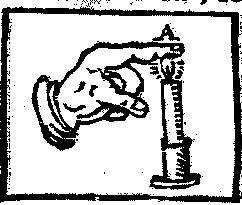
\includegraphics[max width=0.82\textwidth,max height=0.42\textheight,keepaspectratio]{images/figura16.png}\vspace{0.4em}\end{center}


\textit{Quì autem fieri possit, vt ex hac digiti interpositione aspectus flammæ non impediatur, sic ostendo. Cum oculi pupilla indiuisibilis non sit, sed plures possit in partes diuidi; poterit vna illius pars tegi, reliquis non tectis; quamuis ergò, parte aliqua pupillæ obtecta, ad illam species obiecti luminis non perueniant; si tamen reliquæ apertæ remaneant, \& ad illas eædem species pertingere possint, lumen adhuc videbitur.}


\begin{center}\vspace{0.4em}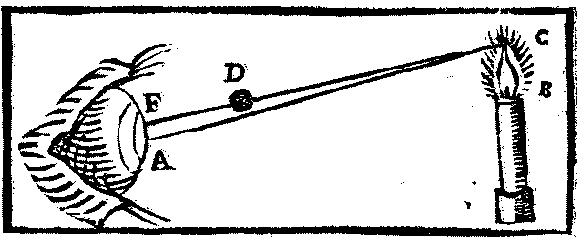
\includegraphics[max width=0.82\textwidth,max height=0.42\textheight,keepaspectratio]{images/figura17.png}\vspace{0.4em}\end{center}


\textit{Sit enim, verbi gratia lumen BC, oculi pupilla FA, corpus opacum interpositum sit D, quod quidem speciem puncti C, peruenire ad F, non permittat; nullo tamen sit impedimento, quìn ex C, alter radius CA, perueniat ad partem pupillæ A; per radium ergo CA, videbitur apex luminis C; non videbitur autem adeò fulgens, vt tunc, quando totam pupillam sua imagine explebat. idem autem apex C,non priùs videri desinet, quàm corpus D, totam pupillam tegat, prohibeatque, nè vllis radijs apex C, ad illam feratur. Quòd si corpus D, multò minus fuerit, quàm oculi pupilla, verbi gratia, filum aliquod crassum, parumque ab eadem pupilla abfuerit, lumine interim longe posito; quomodocunqne inter oculum, \& lumen idem filium extendatur, nullam luminis partem impediet, neque fili eiusdem pars, inter oculum, \& flammam constituta, comparebit, ac si prorsus combusta fuisset; quod ex eadem causa oritur. Neque enim filum illud, }\textit{cum minus sit, quàm pupilla, si ab eadem non longè distet impedire potest quominus omnes flammæ partes, aliquibus saltem radijs, ad potentiam ferantur: quare per eos saltem flamma videbitur. }\textit{Ad tertium denique dictum, quo ait, sidera hoc splendore accidentario spoliari, cum Tubo optico conspiciuntur, multa hic etiam sunt, quæ non facilè soluantur. Nam si Tubus opticus sidera adscititio hoc fulgore spoliaret;}\textit{ }\textit{non deberet hic fulgor per Tubum conspici: at conspicitur tamen. Et quidem inter fixas stellas, nulla est adeò exigua, quæ splendore isto, etiam non suo, à Tubo exui patiatur; quod Galilæus ipse fateri videtur, dum à Cane alijsque stellis, fulgorem illum nunquam omnino auferri posse affirmat. semper enim, etiam per Tubum, scintillantes hosce radios in illis intuemur. Sed quid dico à stellis? Planetæ etiam aliqui adeò fulgoris huius tenaces sunt, vt nunquam sibi illum eripi patiantur; Mars videlicet, Venus, atque Mercurius; quorum lumen, nisi coloratis vitris, specillo aptatis, retuderis, nunquam nudi comparebunt. Et sanè non video, si eadem radiorum illorum causa in superficie oculi remanet, hoc est humor ille pupillæ perpetuò insidens; cur postea, si lumen Astri, per specilli vitra refractum, in eumdem humorem incidat, refringi iterùm, quanquam diuerso fortasse modo, eosdemque luminis ductus producere non debeat. Iam verò si illud admittatur, quod admitti necesse est, vt suprà probauimus, Aërem etiam illuminari, atque ex hoc fieri posse, vt sidus maius appareat, quàm reuerà sit; non poterit Galilæus negare, ex hoc saltem capite, circumfusum etiam fulgorem videri per Tubum, atque ab eodem augeri, quæ vltrà ipsum posita sunt. cum igitur hic etiam splendor vltrà specillum sit, per illud conspici, augerique debebit. Quòd si }\textit{nihilominus in Stellis hoc incrementum non percipitur, aliunde petenda erit huius aspectus causa, non ex eo, quòd radiatio hæc fiat inter specillum, \& oculum, hoc est in superficie humida oculi. Hoc enim, si non de radijs illis vagis, ac distinctis, sed de stabili, \& continuo amplioris luminis coronamento loquamur; ex Aëre illuminato existere posse, Solis, ac Lunæ exemplis, propè Horizontem ampliori orbe, quàm in vertice, apparentium, comprobatur. Si verò de radijs }\textit{ipsis intelligatur: cum hi etiam per specillum conspiciantur in Stellis; non poterit hoc minimum earumdem Stellarum incrementum, in radiorum illorum abiectionem referri, cum non abijciantur.}


Passi ora V. S. Illustrissima alla terza proposizione, la quale legga e rilegga tutta con attenzione; dico con attenzione, acciò tanto più manifestamente si conosca poi, quanto artificiosamente vada pure il Sarsi continuando suo stile di voler coll'alterare, leuare, ed aggiungere, e più col diuertire il discorso e meschiarlo con cose aliene dal proposito, offuscar la mente del lettore, si che in vltimo, trà le cose da se confusamente apprese gli possa restar qualche opinione, che il Signor Mario non abbia così stabilita la sua dottrina, che altri non v'abbia potuto trouar che opporre. Essendo stata opinione di molti, ch'vna fiammella ardente apparisca assai maggiore in certa distanza perch'ella accenda, ed in conseguenza renda egualmente splendida buona parte dell'aria sua circonuicina, onde poi da lontano, è l'aria accesa, e la vera fiammella appariscano vn lume solo; Il Signor Mario confutando questo disse, che l'aria non s'accendeua, nè s'illuminaua, e che l'irraggiamento, per cui si faceua l'ingrandimento, non era intorno alla fiammella, mà nella superficie dell'occhio nostro. Il Sarsi, volendo trouar, che opporre à cotal vera dottrina, in vece di render grazie al Signor Mar. d'auergli insegnato quello, che di sicuro gli era sino allora stato ignoto, si fà innanzi, e si pone à voler prouare, come contro al detto del Signor Mar. l'aria s'illumina, nella quale impresa egli per mio parere, erra in molte maniere. E prima, doue il Signor Mar. redarguendo il detto di quei Filosofi disse, che l'aria non s'accendeua, nè s'illuminaua, il Sarsi mette sotto silenzio quella parte dell'accendersi, e solo tratta dell'illuminarsi, onde il Sig. Mar. con ragion può dire al Sarsi d'auer parlato d'vna cosa, ed esso auer preso ad impugnarne vn'altra, auer parlato dico dell'aria circonuicina alla fiammella, e dell'illuminazione, che le può venire dal suo accendersi, e quello auer parlato dell'illuminazione, che senza incendio viene sopra l'aria vaporosa, posta in qualsiuoglia distanza dall'oggetto illuminante. Inoltre egli medesimo sul primo ingresso dice, che i corpi diafani non s'illuminano, tra i quali mette nel primo luogo l'aria, e poi soggiunge, che mescolata con vapori grossi, e potenti à riflettere il lume, ella ben s'illumina. Adunque Sig. Sarsi sono i vapori grossi, e non l'aria, quelli, che s'illuminano. Voi mi fate souuenir di quello, che diceua, che il grano gli faceua venir capogiroli, e stornimenti di testa, quando però v'era mescolato del loglio. Mà è il loglio, in buon'ora, e non il grano, quello ch'offende. Voi volete insegnarci, che nell'aria vaporosa s'illumina l'Aurora, che mill'altri, ed il Sig. Mar. stesso l'hà in sei luoghi scritto innanzi à voi? Ma che più, voi medesimo in questo medesimo luogo dite, che io l'ammetto insino intorno alla Luna, ed à Gioue, adunque tutte le proue, ed esperienze di Aurora, d'Aloni, di Parelij, e di Luna ascosta dopò qualche parete, sono superflue, non auendo noi giamai dubitato, non che negato, che i vapori diffusi per aria, le nuuole, e la caligine s'illuminano. Mà che volete voi Sig. Sarsi, far poi di cotale illuminazione? dir forse (come in effetto dite) che per essa appariscano i primarij oggetti illuminati maggiori? e come non v'accorgete voi, che, quando ciò fusse vero, bisognerebbe che il Sole, e la Luna si mostrassero grandi, quanto tutta l'Aurora e gli Aloni interi, imperòche cotanta è l'aria vaporosa, che del lume loro è fatta partecipe? Voi dunque Sig. Sarsi, perche auete trouato scritto (dico così, perche voi stesso citate i Filosofi, e gli Autori d'Ottica, per confermare, ed autorizare cotali proposizioni) che la Region vaporosa s'illumina, ed oltre à ciò, che il Sole, e la Luna vicini all'orizonte appariscono mediante tal Regione vaporosa maggiori, che inalzati verso il mezo Cielo vi siete persuaso, che da cotale illuminazione dependa il loro apparente ingrandimento. È vera l'vna, e l'altra propositione, cioè, che l'aria vaporosa s'illumina, e che il Sole, e la Luna presso all'Orizonte, mercè della Region vaporosa appariscono maggiori; ma è falso il connesso delle due proposizioni, cioè che la maggioranza dipenda dall'esser tal Regione illuminata, e voi vi sete molto ingannato, e toglieteui da così erronea opinione; imperocchè, non pel lume de' vapori, ma per la figura Sferica dell'esterna loro superficie, e per la lontananza maggiore di quella dall'occhio nostro, quando gli oggetti son più verso l'Orizonte appariscono essi oggetti maggiori della lor commune apparente grandezza, e non i luminosi solamente, mà qualunque altro posto fuor di tal Regione. Traponete tra l'occhio vostro, e qualsiuoglia oggetto vna lente conuessa cristallina in varie lontananze, vedrete, che quando essa lente sarà vicino all'occhio, poco si accrescerà la specie dell'oggetto veduto, mà discostandola, vedrete successiuamente andar quella ingrandendosi. E perche la Region vaporosa termina in vna superficie sferica non molto eleuata sopra il conuesso della Terra, le linee rette, che tirate dall'occhio nostro arriuano alla detta superficie, sono disuguali, e minima di tutte la perpendicolare verso il vertice, e dell'altre di mano in mano maggior sono le più inclinate verso l'Orizonte che verso il Zenit; Quindi anco (\& sia detto per transito) si può facilmente raccorre la causa dell'apparente figura ouata del Sole, e della Luna presso all'orizonte, considerando la gran lontananza dell'occhio nostro dal centro della Terra ch'è lo stesso, che quello della sfera vaporosa; della quale apparenza, come credo, che sappiate, ne sono stati scritti, come di Problema molto astruso interi trattati, ancorche tutto il misterio non ricerchi maggior profondità di dottrina che l'intender per qual ragione vn cerchio veduto in maestà ci paia rotondo, mà guardato in iscorcio ci apparisca ouato. Mà ritornando alla materia nostra, io non sò con che proposito dica il Sig. Sarsi, esser cosa ridicolosa il dire, che l'Alba, e i crepuscoli, ed altri simili splendori si generino nell'vmore sparso sopra l'occhio, e molto più ridicoloso, se alcuno dicesse, che guardando noi verso il vertice, auessimo gli occhi più secchi, che guardando l'orizonte, e che però la Luna, e 'l Sole ci paresser minori in quel luogo, che in questo, non sò dico à che fine sieno introdotte queste sciocchezze, non si trouando chi già mai l'abbia dette, mà mentre il Sarsi ci figura per troppo semplici, veggiamo se forse cotal nota più ad esso, che à noi s'accommodi. Qui si tratta di quello irraggiamento auuentizio, per lo quale le Stelle, ed altri lumi inghirlandandosi appariscono assai maggiori, che se fussero visti i loro piccoli corpicelli spogliati di tali raggi, trà i quali, perche sono poco men lucidi della prima, e vera fiammella, resta esso corpicello indistinto in modo, che, ed esso, e l'irraggiamento si mostra, come vn sol'oggetto grande, e risplendente. A parte di questo irraggiamento, ed ingrandimento vuole il Sarsi mettere il lume, che per refrazzione si produce nell'aria vaporosa, e vuole, che per questo il Sole, e la Luna si mostrino maggiori verso l'orizonte, che eleuati in alto, e, quel, ch'è peggio vuole, che l'istesso abbiano creduto molti altri Filosofi: il che è falso, nè anno si altamente errato. E che questo sia grandissimo errore, lo doueua molto speditamente mostrare al Sarsi la grandissima distinzione, che si vede trà le luci del Sole, e della Luna, e l'altro splendore circunfuso, dentro al quale incomparabilmente più lucido, e meglio determinato questo, e quel luminare si discerne; il che non accade dell'irraggiamento delle Stelle, tra 'l quale il corpicello della stella resta da pari splendore ingombrato ed indistinto. Mà sento il Sarsi, che risponde, e dice, che quel Sole, e Luna grandi non sono i corpi reali nudi, e schietti, mà vno aggregato, e composto del piccol corpo reale e dell'irraggiamento, che l'inghirlanda e racchiude in mezo, con luce non minore della primaria, onde ne risulta il gran disco apparente tutto egualmente splendido. Mà se questo è, S. Sarsi, perche non si mostra la Luna cosi grande nel mezo del cielo ancora, vi manca forse l'aria vaporosa atta ad illuminarsi io non sò quello, che voi foste per rispondere, nè me lo potrei immaginare, perche non si potendo contra à vn vero venir con altro, che con fallacie, e chimere, le quali, come voi sapete, sono infinite, io non potrei indouinar la vostra eletta. Mà per troncarle tutte in vna volta, e cauar voi, ed, altri, se vi fussero, d'errore, basti à farui taccar con mano che la gran Luna, che voi vedete nell'orizonte è la schietta, e nuda, e non aggrandita per altra luce auuentizia, e circunfusa, basti, dico, il vedere le sue macchie sparse per tutto il suo disco sino all'estrema circonferenza nella guisa à capello, che si mostra nel mezo del Cielo; che se fusse, come auete creduto voi, le macchie nella Luna bassa, e grande, si douerebbon veder raccolte tutte nella parte di mezo, lasciando la ghirlanda intorno lucida, e senza macchie. Adunque non per isplendore aggiunto, mà per vno ingrandimento di tutta la specie nel refrangersi nella remota superficie vaporosa si mostrano il Sole, e la Luna maggiori bassi, che alti.


Or vedete, Sig. Sarsi, quanto è facil cosa l'atterrare il falso e sostenere il vero. Questa pur troppo grand'euidenza della falsità di molte Proposizioni che si leggono nel vostro libro, non mi lascia interamente credere, che voi non l'abbiate compresa, e vò pensando, che possa essere, che, conoscendoui voi internamente dalla realtà delle ragioni conuinto, vi riduciate per vltimo partito à far proua se l'auuersario col creder vere quelle cose, che voi stesso conoscete false, si ritirasse, e cedesse; e che perciò voi arditamente le portiate auanti, imitando quel giocatore, che vedendosi d'auer à carte scoperte perduto l'inuito, tenta con altro soprinuito maggiore di far credere all'auersario gran punto quello, che piccolissimo vede egli stesso, onde cacciato dal timore ceda, e se ne vada, e perche io veggo che voi vi siete alquanto intrigato trà questi lumi primarij, refratti; e reflessi, ne' vapori, ò nell'occhio, comportate voi, come scolare, ch'io come professore, e mæstro vecchio, vi suiluppi ancora vn poco meglio. Per tanto sappiate, che dal Sole, dalla Luna, e dalle Stelle, corpi tutti risplendenti e constituiti fuori, e molto lontani dalla superficie della Region vaporosa, esce splendore, che perpetuamente illumina la metà di tal Regione, e di questo emisferio illuminato l'estremità occidentale, ci arreca la mattina l'Aurora, e la parte opposta ci lascia la sera il crepuscolo: mà niuna di queste illuminazioni accresce, ò scema, ò in modo alcuno altera l'apparente grandezza del Sole, Luna, e stelle che perpetouamente si ritrouano nel centro, ò vogliamo dir nel Polo di questo emisferio vaporoso da loro illuminato; del quale le parti direttamente trapposte trà l'occhio nostro e 'l Sole, ò la Luna, ci si mostrano più splendide dell'altre, che di grado in grado da queste parti di mezo più si discostano, lo splendor delle quali và di mano in mano languendo; e questo è quel lume, che dà segno dell'appressamento della Luna allo scoprirsi, mentre dopo qualche tetto, ò parete ci si nasconde, vna simile illuminazione si fanno intorno intorno anco le fiammelle poste dentro alla sfera vaporosa, mà questa è tanto debile e languida, che se di notte asconderemo vn lume dopò qualche parete, e poi ci anderemo mouendo per iscoprirlo, difficilmente scorgeremo splendore alcuno circonfuso, ò vedremo altra luce, sin che si scuopra la fiamma principale, e questo debolissimo lume nulla assolutamente accresce la visibile specie di essa fiammella. Ci è vn'altra illuminazione, fatta per refrazzione nella superficie vmida dell'occhio, per la quale l'oggetto reale ci si mostra circondato da vn cerchio luminoso, mà inferiore assai di splendore alla primaria luce: e questo si mostra allargarsi per maggiore, ò minore spazio non solamente secondo la maggiore, ò minor copia d'umore, mà secondo la cattiua, ò buona disposizion dell'occhio, il che hò io in mè stesso osseruato, che per certa affezzione cominciai à vedere intorno alla fiamma della candela vno Alone luminoso, e di Diametro di più d'vn braccio, e tale, che mi celaua tutti gli oggetti posti di là da esso, scemando poi l'indisposizione, scemaua la grandezza, e la densità di questo Alone, mà però me ne resta ancora molto più di quello, che veggono gli occhi perfetti; e questo Alone non s'asconde per l'interposizion della mano, ò d'altro corpo opaco, trà la candela, e l'occhio, mà resta sempre trà la mano, e l'occhio, sinche non si occulta il lume stesso della candela; per questo lume parimente non s'ingrandisce la specie della fiammella, del cui splendore egli è assai men chiaro. Ci è vn terzo splendore vivacissimo, e chiaro quasi al par dell'istesso lume principale, il qual si prodduce per riflessione de' raggi primarij fatta nell'vmidità de gli orli, ed estremità delle palpebre, la qual riflessione si distende sopra 'l conuesso della pupilla, della qual prodduzzione abbiamo argomento sicuro dal mutar noi la positura della testa; imperoche secondo, che noi la inchineremo, alzeremo, ò vero terremo dirittamente opposta all'oggetto luminoso, lo vederemo irraggiato nella parte superiore solamente, ò nell'inferiore solamente, ò in ambedue; mà dalla destra, ò dalla sinistra, giamai non vederemo comparirgli raggi, perche le riflessioni fatte verso gli angoli dell'occhio non possono arriuar sopra la pupilla, sotto l'orizonte della quale, mediante la piegatura delle palpebre sù la sfera dell'occhio, esse parti angolari si ritrouano. E se altri calcando colle dita sopra le palpebre, allargherà l'occhio, e discosterà gli orli di quelle dalla pupilla, non vedrà raggi, nè sopra, nè sotto, auuenga, che le reflessioni fatte in essi orli non vanno sopra la pupilla. Questo solo è quello irraggiamento, per lo quale i piccoli lumi ci appariscono grandi, e raggianti, e nel quale la real fiammella resta ingombrata, ed indistinta. L'altre illuminazioni non anno, S. Sarsi che far nulla, nulla \textit{pænitus}, nell'ingrandimento, perche sono tanto inferiori di luce al lume primario, che ben sarebbe cieco affatto, chi non vedesse il termine; confine, e distinzione trà l'vno, e l'altro, oltre che (come di sopra hò detto) il Disco del Sole, e quel della Luna, quando per tale illuminazione s'ingrandissero, dourebbono mostrarsi grandi, quanto gl'immensi cerchi delle loro Aurore. Però quando voi dite, che non negate quella corona raggiante esser affezzion dell'occhio, mà che non perciò hò io ancora prouato, che qualche parte non dipenda dall'aria circunfusa illuminata, toglieteui dal troppo miseramente mendicar sussidij così scarsi. Che volete che faccia quel debolissimo lume mescolato con quei fulgentissimi raggi reflessi dalle palpebre? aggiunge quel, che farebbe il lume d'vna torcia à quel del Sole meridiano. Di questo lume sparso per l'aria vaporosa, io ve ne voglio conceder non solamente quella piccola parte che voi domandate, mà quanto abbraccia tutta l'Aurora, e 'l crepuscolo, e tutto l'emisferio vaporoso, e di questo voglio, che il corpo luminoso, nè per Telescopio, nè per altro mezo possa giamai essere spogliato, e voglio ancora per vostra compitissima soddisfazzione, ch'ei venga dal Telescopio ingrandito, come tutti gli altri oggetti, si che non pure adegui tutta l'Aurora, mà mille volte maggiore spazio, se mille volte tanto si potesse comprendere coll'occhiale. Mà niuna di queste cose solleua punto, nè voi, nè 'l vostro maestro, che aureste bisogno per mantenimento della vostra principal conchiusione, ch'è, che le Stelle fisse per esser lontanissime non riceuono accrescimento veruno dal Telescopio, aureste bisogno dico, che la Stella, ed il suo irraggiamento fusse vna cosa medesima; ò almeno, che l'irraggiamento fusse realmente intorno alla Stella; mà ne quello, ne questo è vero, mà bene è egli nell'occhio, e le Stelle riceuono accrescimento tanto, quanto ogn'altro oggetto veduto col medesimo strumento, come puntualissimamente scrisse, e dimostrò il Sig. Mario. Questi altri vostri diuerticoli d'arie vaporose illuminate, e di Soli, e Lune alte, e basse, son, come si dice, pannicelli caldi, e vn voler fuggir la scuola, e cercar di deuiare il lettore dal primo proposito. e frà l'altre vostre molte diuersioni, questa, che fate in mostrar con assai lungo discorso, come per l'interposizion del dito non s'impedisca la vista della fiammella, e quel, che dite del filo sottile, e del corpo interposto minor della pupilla son tutte cose vere, ma per mio auuiso nulla attenenti al proposito, che si tratta, il che veggo, che internamente auete conosciuto voi medesimo ancora, atteso, che quando era il tempo dell'applicazione di queste cose alla materia, e di chiuder la conchiusione, voi fate punto; e lasciandoci sospesi passate ad altro proposito, e cercate pur per via di discorso prouar cosa di cui cento esperienze chiarissime sono in contrario, e benche voi veggiate guardando col Telescopio la Stella di Saturno terminatissima, e di figura diuersissima dall'altre, il Disco di Gioue, e quel di Marte, e massime quando è vicino à terra, perfettamente rotondi, e terminati, Venere a' suoi tempi corniculata, ed esattissimamente delineata, i globetti delle Stelle fisse, e massime delle maggiori molto ben distinti, e finalmente mille fiammelle di candele poste in gran distanza così ben distornate, come da vicino, doue senza il Telescopio l'occhio libero niuna di cotali figure distingue, mà tutte le vede ingombrate da raggi stranieri, e tutte sotto vna stessa figura radiante: con tutto ciò pur volete che 'l Telescopio non le mostri senza raggi, persuaso da certi vostri discorsi, de i quali, io non sarei in obligo di scoprir le fallacie, auendo per me l'esperienza in contrario, tuttauia, per vostra vtilità, le accennerò così brevemente, e per venir con ogni maggior chiarezza al mio intento, io vi domando Sig. Sarsi, onde auuenga, che Venere si circonda sì fattamente di questi raggi ascitizij, e stranieri, che trà essi perde in modo la sua real figura, ch'essendo stato dalla creazion del mondo in quà mille, e mille volte cornicolata, mai da viuente alcuno non è stata osseruata, ne veduta tale, mà sempre è apparsa d'vna stessa figura, se non dapoi ch'io primieramente col Telescopio scopersi le sue mutazioni? il che non accade della Luna, la quale coll'occhio libero mostra le sue diuersità di figure, senza notabile alterazione, che dipenda dall'irraggiamento auuentizio. Non rispondete, ciò accadere mediante la gran lontananza di Venere, e la vicinanza della Luna; perche io vi dirò, che quello, che accade à Venere, accade ancora alle fiammelle delle candele, le quali in distanza di cento braccia solamente confondono la lor figura trà i raggi, e la perdono non men di Venere. Se volete risponder bene, bisogna che diciate ciò deriuare dalla piccolezza del corpo di Venere, in relazione all'apparente grandezza di quel della Luna; e che vi figuriate la lungezza di quei raggi, che si prodducono nell'occhio esser, v. gr. per quattro Diametri di Venere, che non saranno poi la decima parte del Diametro della Luna. Ora figurateui la piccolissima falce di Venere inghirlandata di vna chioma, che se le sparga e distenda intorno intorno in distanza di quattro suoi diametri, ed insieme la grandissima falce della Luna con vna chioma non più lunga della decima parte del suo diametro; non douerà esserui difficile à intendere, come la forma di Venere del tutto si perderà trà la sua capellatura, mà non già quella della Luna, la quale pochissimo s'altererà: ed accade in questo quello à punto, che accaderebbe in vestire vna formica di pelle d'agnello, di cui la configurazione delle piccoline membra in tutto, e per tutto si perderebbe, trà la lungezza de i peli, si che l'istessa apparenza farebbe, che se fusse vn bioccolo di lana; nulla dimeno l'Agnello per la sua grandezza assai distinte mostra le membra sue sotto la pecorile spoglia. Mà dirò di più, che riceuendo il capillizio splendido, che risiede nell'occhio la limitazion del suo spargimento dalla costituzion dell'occhio stesso, più che dalla grandezza dell'oggetto luminoso, e così veggiamo stringendo le palpebre, si che appariscano sopra dall'oggetto luminoso raggi molto lunghi, non si veggono maggiori quei, che vengono dalla Luna, che quei di Venere, ò d'vna torcia, ò d'vna fiaccola figurateui vna diterminata grandezza d'vna capellatura, nel mezo della quale se voi intenderete essere vn piccolissimo corpo luminoso, perderà la sua figura coronato di troppo lunghi crini; mà ponendoui vn corpo maggiore, e maggiore, finalmente potrà il simulacro reale occupar tanto nell'occhio, che poco, ò niente gli auanzi intorno del capillizio; e così l'immagine, v. gr. della Luna potrà esser, che ingombri nell'occhio spazio maggiore della commune irradiazione. Stante queste cose intendete il disco reale, per essempio, di Gioue, occupar sopra la nostra luce vn cerchietto, il cui diametro sia la ventesima parte dello spargimento della chioma raggiante, onde in si gran piazza resta indistinto il piccolissimo cerchietto reale; viene il Telescopio, e m'aggrandisce la specie di Gioue in Diametro venti volte; mà già non ingrandisce l'irraggiamento, che non passa per li vetri: adunque io vedrò Gioue non più, come vna piccolissima Stella radiante, mà come vna Luna rotonda, ben grande, e terminata; e se la Stella sarà assai più piccola di Gioue, mà di splendore molto fiero, e viuo, qual è per essempio il Cane, il cui diametro non è la decima parte di quel di Gioue, nulla di meno la sua irradiazione è poco minor di quella di Gioue, il Telescopio accrescendo la Stella, mà non la chioma, fà che doue prima il piccolissimo disco trà sì ampio fulgore era impercettibile già fatto in superficie 400. e più volte maggiore si può distinguere, ed assai ben figurare. Con tal fondamento andate discorrendo, che potrete disbrigarui per voi stesso da tutti gl'intoppi. E rispondendo alle vostre instanze, quando dal Sig. Mario, e da me è stato detto che 'l Telescopio spoglia le Stelle di quel coronamento risplendente, ciò è stato profferito non con intenzione d'auere à stare à sindicato di persone così puntuali, come siete voi, che non auendo altro, doue attaccarui, vi conducete sino à dannar con lunghi discorsi chi prende il termine vsitatissimo d'infinito per grandissimo. Quando noi abbiamo detto, che il Telescopio spoglia le Stelle di quello irraggiamento, abbiamo voluto dire, ch'egli opera intorno à loro in modo, che ci fà vedere i lor corpi terminati, e figurati, come se fussero nudi, e senza quello ostacolo, che all'occhio semplice asconde la lor figura. E egli vero Sig. Sarsi, che Saturno, Gioue, Venere, e Marte all'occhio libero non mostrano trà di loro vna minima differenza di figura, e non molto di grandezza seco medesimi in diuersi tempi? e che coll'occhiale si veggono, Saturno, come appare nella presente figura, e Gioue, e Marte in quel modo sempre; e Venere in tutte queste forme diuerse? e, quel, ch'è più merauiglioso con simile diuersità di grandezza? si che cornicolata mostra il suo disco 40. volte maggiore, che rotonda, e Marte 60. volte quando è perigeo, che quando è apogeo, ancorche all'occhio libero non si mostri più che 4. o 5.?


\begin{center}\vspace{0.4em}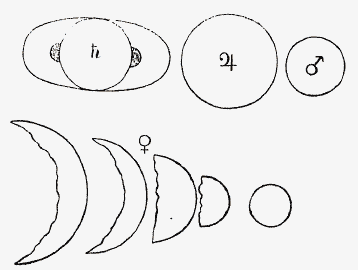
\includegraphics[max width=0.82\textwidth,max height=0.42\textheight,keepaspectratio]{images/figura18.png}\vspace{0.4em}\end{center}


Bisogna, che rispondiate di si, perche queste son cose sensate, ed eterne, si che non si può sperare di poter per via di sillogismi dare ad intendere, che la cosa passò altrimenti. Or l'operare col Telescopio intorno à queste Stelle in modo, che quell'irraggiamento, che perturbaua l'occhio libero, ed impediua l'esatta sensazione, la qual'opera è cosa massima, e d'ammirabili e grandissime conseguenze, è quello, che noi abbiam voluto significare nel dire, \textit{spogliar le Stelle dell'irraggiamento}, che son parole solamente di niun momento, di niuna conseguenza; le quali se à voi che siete ancora scolare, danno fastidio, potrete mutarle à vostro beneplacito, come cambiaste già quello nostro accrescimento nel vostro transito dal non essere all'essere. A quello che voi dite parerui pur ragionevole, che si come l'oggetto lucido venendo per lo mezo libero prodduce nell'occhio l'irraggiamento, egli debba ancor far l'istesso, quando viene passando per li christalli del Telescopio; rispondo concedendouelo liberamente, e dicoui, che accade apunto l'istesso de gli oggetti veduti col Telescopio che de' veduti senza; e si come il disco di Gioue per essempio veduto coll'occhio libero rimane per la sua piccolezza perduto nell'ampiezza del suo irraggiamento, mà non già quello della Luna, che colla sua gran Piazza occupa sopra la nostra pupilla spazio maggiore del cerchio raggiante, per lo che ella si vede rasa, e non crinita, così facendomi il Telescopio arriuar sopra l'occhio il disco di Gioue sei cento, e mille volte maggiore della specie sua semplice, fà ch'egli colla sua ampiezza ingombri tutta la capellatura de' raggi, e comparisca simile ad vna Luna piena, mà il disco piccolissimo del cane, benche mille volte ingrandito dal Telescopio, non però adegua ancora la piazza radiosa, si che ci apparisca tosato del tutto; nientedimeno, per essere i raggi verso l'estremità alquanto men forti, e trà loro diuisi resta egli visibile, e trà la discontinouazion de' raggi si vede assai commodamente la continouazion del globetto della Stella, il quale con vno strumento, che più, e più l'accrescesse, più, e più sempre distinto, e meno irraggiato ci si mostrerebbe, si che la cosa Sig. Sarsi stà così, e questo effetto ci venne chiamato vno spogliar Gioue del suo capillizio; le quali parole se non vi piacciono, già vi si è dato licenza, che le mutiate ad arbitrio vostro, ed io vi dò parola d'vsar per l'auuenire la vostra correzzione; mà non v'affaticate in voler mutar la cosa, perche non farete niente. E già che voi in questo fine replicate, che pure è necessario conceder, che l'aria circunfusa s'illumini, e che perciò la Stella apparisca maggiore, ed io torno à replicarui, che i vapori circunfusi s'illuminano, mà non perciò il corpo luminoso s'accresce punto, essendo che il lume de' vapori è incomparabilmente minore della primaria luce, per lo che il corpo lucido, se è grande, resta nudo, e se è piccolo, rimane col suo irraggiamento fatto nell'occhio, terminatissimo, e distintissimo, tra 'l debolissimo lume dell'aria vaporosa; e vi replico ancora, poiche voi medesimo me ne porgete replicata occasione, che totalmente depogniate quella falsa opinione, che 'l Sole, e la Luna presso all'orizonte si mostrino maggiori per vna ghirlanda d'aria illuminata, che s'aggiunga al lor disco, perche questa è vna grandissima semplicità, come di sopra hò detto, e prouato. E per non lasciar cosa intentata per cauarui d'errore, e far, che voi restiate capace di questo negozio, alle vostre vltime parole, doue voi dite, che vedendosi pur pel Telescopio essi raggi luminosi intorno alle Stelle, non si potrà ridurre il minimo ricrescimento di quelle nella perdita di questi, essendo, che non si perdono, vi rispondo, che l'accrescimento è grandissimo, come in tutti gli altri oggetti, e che il vostro errore stà (come sempre si è detto) nel paragonar voi la Stella insieme con tutto il suo irraggiamento visto coll'occhio libero col corpo solo della Stella veduto collo strumento distinto dalla sua piazza radiosa, della quale egli taluolta compar maggiore, e tal volta eguale, secondo la grandezza della Stella vera, e la moltiplicazion del Telescopio, e quando comparisce minor di esso irraggiamento, tuttauia si scorge il suo Disco, come hò detto, trà l'estremità della capellatura. Ed vna accommodatissima riproua dell'accrescimento grande, come in tutti gli altri oggetti, è il pigliar Gioue coll'occhiale auanti giorno, e andarlo seguitando sino al nascer del Sole, e più oltre ancora; doue si vede il suo Disco pel Telescopio sempre grande nell'istesso modo, mà quel che si vede coll'occhio libero, crescendo il candor dell'Aurora, si và sempre diminuendo, si che vicino al nascer del Sole, quel Gioue, che nelle tenebre, superaua d'assai ogni Stella della prima grandezza, si riduce ad apparir minore di quelle della quinta, e della sesta, e finalmente, ridottosi quasi ad vn punto indiuisibile nascendo il Sole si perde del tutto; nulla dimeno sparito all'occhio libero, si seguita egli pur di vederlo tutto il giorno grande, e ben circolato; ed io hò vno strumento, che me lo mostra, quando è vicino alla Terra, eguale alla Luna veduta liberamente; Non è dunque cotal ricrescimento minimo, ò nullo, mà grande, come di tutti gli altri oggetti. Io vi voglio Sig. Sarsi pigliare alla stracca, se non potrò prenderui correndo. Volete voi vna nuoua dimostrazione per proua, che gli oggetti in tutte le distanze crescono nella medesima proporzione? Sentitelo. Io vi domando se posti quattro, sei, ò dieci oggetti visibili in varie lontananze, mà in guisa però, che tutti si veggano nella medesima linea retta, si che il più vicino occupi tutti gli altri, vi domando dico, se tenendo l'occhio nel medesimo luogo, e riguardando i medesimi oggetti co 'l Telescopio, voi gli vedrete pur posti in linea retta, ò nò, si che il vicino non vi asconda più gli altri; mà ve gli lasci vedere? credo pur, che voi risponderete, ch'ei vi compariranno per linea retta, essendo realmente per linea retta disposti. Ora stante questo, immaginateui quattro, sei, ò dieci bacchette diritte, trà di lor paralelle, poste in distanze dissuguali dall'occhio, ed esse di lunghezze pur disuguali e le più lontane maggiori, e di mano in mano le più vicine minori in modo, che gli estremi termini loro si veggano posti in due linee rette, vna à destra e l'altra à sinistra; pigliate poi il Telescopio, e riguardatele con esso, già per la concession fatta i medesimi termini, tanto i destri, quanto i sinistri, si vederanno pure in due linee rette come prima, mà aperte in maggiore angolo. E come ciò sia Sig. Sarsi, questo appresso i Geometri si domanda ricrescer tutte quelle linee secondo la medesima proporzione, e non ricrescer più le vicine, che le lontane, cedete dunque, e tacete.



\par\bigskip\noindent\phantomsection\addcontentsline{toc}{section}{§ 50}{\Large\color{rubric}\textbf{50.}}\enspace \textit{Sed videamus, quàm rectè, ex Peripatetica disciplina, atque ex experimentis sibi arma contrà Aristotelem fabricet Galilæus. Præterea, inquit, Cometam flammam non fuisse, ex ipsa experientia, \& Peripateticorum dicto deducimus, quo affirmant, nullum corpus lucidum esse perspicuum. experientia verò docet flammam, vel minimam, vnius candelæ, impedimento esse, quominus obiecta vltra ipsam posita conspiciantur: si ergò Cometam flammam fuisse, quis dixerit, dicendum eidem erit, Stellas, vltra illam positas; ab ea celari debuisse; \& tamen per Cometæ caudam lucidissimè intermicantes easdem Stellas vidimus. Hæc ille: in quibus, mirari satis non possum, hominem magni alioqui nominis, atque experimentorum amantissimum, ea disertè adeò asseuerasse, quæ obuijs vbique experimentis, redargui facile possent. Quamuis enim Peripateticorum dictum, si rectè intelligatur, verissimum sit: }(\textit{omne enim corpus, ad hoc vt illuminetur, vel potius illuminatum appareat, excurrentem vlterius lucem quasi sistere, ac reprehendere debet; perspicuum autem, vtpotè eidem luci peruium, eam }\textit{terminare non potest: ex quo dicendum est, corpus quodcumque, eò clarius illuminandum, quò plus opaci, minusque habuerit perspicui})\textit{, nullus tamen est, qui neget, reperiri corpora partim perspicua, partim opaca, quæ partem lucis aliquam terminent, qua lucida appareant; aliquam verò liberè transire permittant; qualia sunt nubes rariores, Aqua, Vitrum, \& huiusmodi multa, quae \& lumen in superficie terminant, \& ad aliam partem idem transmittunt. }\textit{Quare nihil est, cur ex hoc dicto quidquam momenti suis experimentum Galilæus adiectum putet. }\textit{Experimenta porrò ipsa falsa deprehenduntur. Affirmo igitur, candelæ flammam obiecta vltra se posita, ex oculis non auferre, \& perspicuam esse. Huic primùm dicto adstipulantur sacræ litteræ, cum de Anania, Azaria, ac Misæle in fornacem, Regis iussu, coniectis agunt. Sic enim Regem ipsum loquentem inducunt: Ecce ego video quatuor viros solutos, \& ambulantes in medio ignis, \& nihil corruptionis in eis est; \& species quarti similis filio Dei.}\textit{ }\textit{Ac nè quis existimet id pro miraculo habendum. idem probatur iterùm ex eo, quia in candelæ flamma, medio loco consistens videtur ellychnium, seu nigricans, seu candens. Prætereà cum strues aliqua ingens lignorum incenditur, medias inter flammas semiusta ligna, \& carbones accensos liberè prospectamus: cum tamen sæpè maxima flammatum vis, oculum inter, atque eadem ligna, media consistat; flamma igitur perspicua est.}


\textit{Secundò, quodcunque opacum inter oculum, \& obiectum positum, eiusdem obiecti aspectum impedit, siue magno, siue paruo ab eodem distet interuallo. }\textit{Ita, v. gr. lignum aliquod, siue rem quampiam attingat, siue ab illa multum remoueatur }(\textit{si tamen inter illam, atque oculum substiterit})\textit{, }\textit{eam videri non permittet; quod in flamma non accidit. hæc enim quascumque res, vltra se positas, si non longè distent, sed easdem è proximo vehementer illuminet, semper videri patietur, quod quilibet experiri facilè potest, si legendum aliquid vltra lumen collocauerit, vnius tantùm digiti interuallo, tunc enim characteres illos à flamma obtectos facilè perleget: flamma ergò perspicua est, \& luminosa, quod Galilæus negat, eiusque oppositum, tanquam principium, contra Aristotelem disputaturus, assumit.}


\textit{Quòd si quis quærat, cur obiecta vltra flammam posita, si saltem ab eadem longè semota fuerint, non conspiciantur, hanc ego huius rei causam assigno. quia nimirum obiectum mouens potentiam vehementius, impedit nè videantur obiecta reliqua, ad eamdem potentiam mouendam minus apta, obiecta autem quælibet eò vehementius, cæteris paribus, potentiam mouent, quò sunt lucidiora: quia igitur obiecta, longè vltra flammam posita, multò minus illuminantur, quàm flamma ipsa; ideò hæc potentiam veluti totam explet, obruitque, nec obiecta alia videri permittit: \& proptereà quò obiecta eadem eidem flammæ fiunt propiora, quia tantò magis illuminantur; eò etiam magis apta sunt mouere potentiam; ac proinde tunc conspiciuntur, maiori siquidem illustrata lumine, cum flamma penè ipsa contendunt. Quare si aut flamma obtusiori splendeat lumine, aut obiectum vltrà illam positum, luminosum ex se sit, aut ab alio vehementer illuminatum, nunquam illius aspectum interposita flamma impediet, quamuis longissimè obiectum illud à flamma distet. Hoc etiam quibusdam experimentis confirmare placet.}


\textit{Incendatur distillatum vinum, quod Aquam vitis, vulgò, appellant; eius enim flamma, cum non admodum clara sit, liberam, rerum imaginibus, ad oculum viam relinquet, vt etiam minutissimos quosque characteres perlegi patiatur. Idem accidit in flamma, ex incenso sulphure, excitata, quæ, colorata licet sit, \& crassa, vix tamen quidquam impedimenti eisdem rerum imaginibus affert.}


\textit{Secundò sit licet flamma clarissimo ac micanti lumine, si tamen alterius candelæ lumen vltrà illam collocatum, longe etiam semoueris; inter vicinioris flammæ lucem, remotiorem flammam intermicantem cernes. Cum ergo Stellæ corpora sint luminosa, \& quauis flamma longè clariora; nil mirum, si non potuit earundem aspectus ab interposita Cometæ flamma impediri; ac proindè nihil detrimenti, ex hoc Galilæi argumento, patitur Aristotelis opinio.}


\textit{Tertiò, non luminosa solùm illa, quæ propria fulgent luce, ab interposita flamma velari non possunt, sed nè alia quidem corpora opaca, si tamen ab alio lumine illustrentur. Ita interdiu, si quid aspexeris à Sole illuminatum, nullius interpositu flammæ, impediri eius aspectus poterit. Constat igitur satis superque, flammas perspicuas esse, atque hoc etiam non obstare, quominus Cometa flamma esse potuerit.}


È tempo Illustrissimo Signore di venir à capo di questi pur troppo lunghi discorsi. Però passiamo à questa quarta, \& vltima Propositione. Qui com'ella vede, dice il Sarsi non potersi à bastanza stupire, che io auendo qualche nome d'auueduto osseruatore, ed applicato assai all'esperienze, mi sia ridotto ad affermar constantemente quelle cose, che si possono ageuolissimamente confutare con esperimenti manifesti, ed apparecchiati per tutto, de' quali poi n'apporta molti, ond'egli apparisca altrettanto veridico, e diligente sperimentatore, quant'io mal accorto, e mendace. Dirò prima breuemente quello, che persuase il Signor Mario à scriuere, e me à prestargli assenso, che quando la Cometa fusse vna fiamma, douesse asconderci le Stelle; poi anderò considerando l'esempio, e ragioni del Sarsi; lasciando in vltimo a V. S. Illustrissima il giudicar qual di noi sia più difettoso, e mal'auueduto nel suo esperimentare e discorrere. Considerando noi, il trasparire d'vn corpo, non esser altro, che vn lasciar vedere gli oggetti posti oltre di se, ci persuademmo, che quant'esso corpo trasparente fusse men visibile, tanto potesse meglio trasparere, onde l'aria trasparentissima è del tutto inuisibile; l'acqua limpida, ed i cristalli ben tersi, traposti trà oggetti visibili, poco per sè stessi si scorgono; dal che ci pareua, che assai à proposito si potesse all'incontro inferire, i corpi, quanto più per sè stessi fusser visibili, douer esser tanto meno trasparenti, e perche trà i corpi visibili per se stessi, le fiamme per auuentura pareuano non esser degli infimi, però giudicammo quelle douere esser poco trasparenti, l'autorità poi di Aristotile e de Peripatetici aggiunta à questo discorso ci confermò nell'opinione, circa la qual autorità mi par da notare, come il Sarsi le vuol dare altra interpretazione da quella, che apertamente suonan le parole, e dice, che intesa bene è verissima, e che il senso è, che i corpi, accioche si possano illuminare, non deuon'esser trasparenti; e non, che i corpi lucidi non son trasparenti. Ma se il Sarsi la piglia in quel senso, perche così gli par la Proposizion vera, adunque bisogna, ch'ei lasci l'altro perche in quello gli paia falsa (perche quanto alle parole, meglio si adattano à questo, che à quello) tuttauia egli medesimo poco di sotto, non pure afferma, ma con più esperienze conferma i corpi luminosi impedir la vista delle cose poste oltre di loro, doue scriue: \textit{Nam hæc etiam rerum vltra ipsa positarum aspectum }\textit{impediunt}\textit{;} e quelche segue. Mà tornando al primo discorso, dico, che oltre all'autorità de' Peripatetici, ci confermò ancora più il veder finalmente per esperienza vn vetro infocato impedirci assai la vista degli oggetti, che freddo distintamente ci lascia scorgere, e l'istesso far la fiammella d'vna candela, e massime colla sua superior parte, più lucida dell'inferiore ch'è intorno al lucignolo, la qual è più tosto fumo, non bene infiammato, che vera fiamma. Di più auendo noi osseruato la grossezza del corpo, benche per se stesso non molto opaco, importar tanto, che, v. gr. vna nebbia, la quale in profondità di venti, ò trenta braccia non ci leua la vista d'vn tronco, moltiplicata all'altezza di 200. ò 300. ci toglie del tutto anco la vista del Sole stesso, pensammo non esser lontano dal ragioneuole il creder, che la non trasparenza, ed opacità d'vna fiamma non potesse mai essere così poca, che ingrossata in profondità di centinaia, e centinaia di braccia, non ci douesse impedir l'aspetto delle minute Stelle. Conchiudemmo per tanto la profondità della Chioma della Cometa; che pur bisogna, che sia, non dirò col Sarsi, e suo maestro, 70. miglia, mà al manco tante canne, quand'ella fusse vna fiamma, douerci ascondere le stelle, il che vedendo noi, ch'ella non faceua, ci parue auere argomento assai concludentemente, per prouar ch'ella non fusse vno incendio. Ora il Sarsi, curando poco, ò niente la principal sustanza di tutto questo ragioneuolissimo discorso, appiccandosi à quel sol detto del S. Mar. che la fiammella d'vna candela, non è trasparente, si persuade, e promette la vittoria, tuttauolta, ch'ei possa mostrare la detta fiammella auer pur qualche trasparenza, e dice che chi auuicinerà à quella vn foglio scritto, si che quasi la tocchi, e porrà diligente cura, potrà vedere i caratteri, al che io aggiungo, tuttauolta, ch'ei sia di vista perfettissima, perche io, che però non son losco, stento à poterli vedere, seruendomi anco degli occhiali, quanto più posso da vicino. è ben vero, che oltre alla detta, molt'altre esperienze adduce il Sarsi, trà le quali, e per riuerenza, e per religiosa pietà e per esser'ella di suprema autorità, debbo primieramente far considerazione sopra quella, che il medesimo Sarsi ripone nel primo luogo, pigliandola dalle Sacre lettere, doue insieme co'l Sig. Mar. noto le parole della scrittura precedenti alle citate dal Sarsi, le quali mi par, che dicano, che auanti che il Rè vedesse l'Angelo, e i tre fanciulli camminar per la fornace, le fiamme fussero state rimosse, che tanto mi par che importino le parole del Sacro Testo, che son queste. \textit{Angelus autem Domini descendit cum Azaria, \& socijs eius, et excussit flammam ignis de fornace, \& fecit medium fornacis quasi ventum roris flantem. }\textit{E nota, che dicendo la scrittura,}\textit{ flammam ignis}, par che voglia far distinzione tra la fiamma, e 'l fuoco, e quando poi più a basso si legge, che il Re vede caminar le quattro persone, si fà menzione del fuoco, e non della fiamma. \textit{Ecce ego video quatuor viros solutos et ambulantes in medio ignis}. Mà perche io potrei grandemente ingannarmi nel penetrare il vero sentimento di materie che di troppo grand'interuallo trapassano la debolezza del mio ingegno, lasciando cotali determinazioni alla prudenza de' mæstri in Diuinità, anderò semplicemente discorrendo trà queste inferiori dottrine con protesto d'esser sempre apparecchiato ad ogni decreto de' superiori, non ostante qualsiuoglia dimostrazione ed esperimento che paresse essere in contrario. E ritornando all'esperienze del Sarsi, per le quali ei ci fà vedere trasparir per varie fiamme diuersi oggetti, dice, che posso liberamente concedergli, tutto questo esser vero, ma di nessuno solleuamento alla sua causa, per lo stabilimento della quale non basta, che la fiamma interposta sia profonda vn dito, e che gli oggetti altrettanto vicini gli sieno, nè molto più lontano il riguardante, ò vero che gli oggetti sieno dentro alle stesse fiamme, ed anco nella parte bassa, pochissimo lucida; mà hà di bisogno (altrimenti restarà à piè) di farci toccar con mano, ch'vna fiamma, ancorche profonda centinaia, e centinaia di braccia, e lontanissima dal riguardante, e da gli oggetti visibili, non però ce n'impedisca la veduta; ch'è quanto se dicessimo, che gli faccia di mestier prouare, che la fiamma arrechi assai meno impedimento, che se fusse altrettanta nebbia; la qual nebbia è tale, che trappostane non solo alla grossezza d'vn dito, mà di quattro, e sei braccia non arreca impedimento veruno, mà in profondità di 100. o 200. asconde l'istesso Sole, non che le Stelle. E finalmente io non mi posso contener di riuolgermi vn poco al medesimo Sarsi, che si stupisce del mio inescusabil mancamento nell'vso dell'esperienze. Voi dunque Sig. Sarsi mi tassate per cattiuo sperimentatore, mentre nell'istesso maneggio errate, quanto più grauemente errar si possa? voi auete bisogno di mostrarci, che la fiamma interposta non basta contro alla nostra asserzione, ad occultarci le Stelle; e per conuincerci con esperienze dite, che prouando noi à riguardar'vuomini, tizzoni, carboni, scritture, e candele posti oltre alle fiamme sensatamente gli vederemo, ne mai v'è venuto in pensiero di dirci, che noi prouiamo à guardar le Stelle? e perche in buon'ora, non ci hauete voi detto alla bella prima; interponete vna fiamma trà l'occhio, e qualche Stella, che voi ne più ne meno la vederete? Mancano forse le Stelle in Cielo? e questo è esser destro, ed auueduto sperimentatore? Io vi domando, se la fiamma della cometa è come le nostre, ò d'altra natura? se d'altra natura, l'esperienze fatte nelle nostre non anno forza di conchiudere in quelle, se è come le nostre: poteuate immediatamente farci veder le Stelle per le nostre, lasciando stare i tizzoni, fuoghi, e l'altre cose, e quando dite, che dopo la fiammella d'vna candela si scorgono i caratteri poteuate dire, che si scorge vna Stella. S. Sarsi, chi volesse trattarla, con voi, come si dice mercantilmente, cioè con vna bilancia sottilissima, e giustissima, direbbe, che voi foste in obligo di fare accendere vna fiamma lontanissima, e grandissima, quanto la cometa, e farci per essa veder le Stelle atteso che, e la grandezza della fiamma, e la lontananza dell'occhio da quella importano assaissimo in questo fatto, e se ne deue tener gran conto: mà io per farui ogni ageuolezza, e vantaggio, mi voglio contentare d'assai meno, e voglio prepararui mezi accommodatissimi per vostro bisogno. E prima, perche l'essere la fiamma vicina, all'occhio importa assai per vedere gli oggetti meglio in vece di porla rimota, quanto la cometa, mi contento d'vna distanza di cento braccia solamente, in oltre perche la profondità, e grossezza del mezo similmente importa assaissimo, in vece della grossezza della cometa, ch'è, come sapete, tante centinaia di braccia, mi basta quella di dieci solamente, in oltre perche l'esser l'oggetto, che si hà da vedere lucido, arreca parimente vantaggio grandissimo, come voi medesimo affermate, mi contento, che tale oggetto sia vna Stella di quelle, che si vider per la chioma della nostra Cometa, le quali Stelle per vostro detto in questo luogo sono di gran lunga più chiare di qualsiuoglia fiamma; e poi se con tutti questi tanto per la causa vostra vantaggiosi apparecchi, voi fate vedere per la trasparenza di cotal fiamma la Stella, voglio confessarmi per conuinto, e predicar voi pel più cauto, e sottile sperimentatore del Mondo; mà non vi succedendo, non ricerco altro da voi, se non che col silentio pogniate fine alle dispute, come spero, che siate per fare, perche se mai v'accaderà di veder questa mia scrittura, la qual rimane nell'arbitrio di questo Signore, à chi scriuo, dimostrarla à chi più gli piacerà, vederete, come deue fare chi si piglia per impresa di volere essaminar gli altrui componimenti, ch'è non lasciar cosa veruna, senza considerarla, non (come auete fatto voi) andar à guisa della Gallina cieca dando or qua, hor là tanto del becco in terra, che s'incontri in qualche grano di miglio, da morderlo, e roderlo. E per finir questa parte non potete negar d'auer voi medesimo compreso, e confessato, che dalle fiamme interposte qualche sensibile impedimento, anco per l'occhio vostro ne diriua; imperoche se niente assolutamente d'offuscamento arrecassero, senz'altri auuertimenti, e cautele d'esser gli oggetti più, ò men lontani dalla fiamma, più, ò men lucidi, ed esse fiamme nate più da zolfo, ò d'acquauite, che da paglia, ò da cera, aureste risolutamente detto, sia la fiamma, e l'oggetto qualunque siuoglia, nessuno impedimento ne nasce, mà si vede, come per l'aria libera, e pura: ed oltre à questo, poco più a basso parlando delle cose, che non risplendono per se stesse, come le fiamme, mà sono illuminate da altri, dite che queste ancora impediscono la vista degli oggetti, doue la particola \textit{ancora} mostra, che voi concedete qualche impedimento nelle fiamme; mà che più? se elle non punto impedissero, à chi mai sarebbe caduto in pensiero di dire, ch'elle non sieno trasparenti? ci è dunque anco per voi stesso qualche sensibil offuscazioncella (dico per voi stesso, perche per noi e gli altri l'impedimento è assai grande) e le vostre esperienze son fatte intorno à fiammelle così piccole, che risolutissimamente l'impedimento d'altrettanta nebbia sarebbe stato del tutto insensibile; adunque le vostre fiamme impediscono più, che altrettanta nebbia; mà tanta nebbia, quanta è la profondità della Cometa, vela, e totalmente toglie la vista del Sole; adunque quando la cometa fusse vna fiamma, dourebbe esser bastante ad asconderci il Sole, non che le Stelle, le quali ella non asconde; adunque non è vna fiamma. E perche quanto per sostenere vn falso sono scarsi tutti i partiti, tanto per istabilimento del vero soprabondano i contrari veri. Io voglio accennare à V. S. Illustrissima certo particolare, per lo quale mi par che si confermi l'opinion d'Aristotile esser falsa. Auuenga, che natura di tutte le fiamme conosciute da noi è di dirizzarsi all'in sù, restando il lor principio, e capo nella parte inferiore, se la barba della Cometa fusse vna fiamma, ed il suo capo fusse la materia, ond'ella træsse origine, bisognerebbe, che la chioma direttamente si dirizzasse verso il Cielo, dal che ne seguirebbe vna delle due cose, cioè, ò che la Chioma si vedesse sempre à guisa di ghirlanda intorno al capo, il che sarebbe, quando il luogo della Cometa fusse altissimo, ò vero (e questo accaderebbe, quand'ella fusse poco lontana da Terra) bisognerebbe che nel nascere prima nascesse l'estremità della barba, ed in vltimo il capo, ed alzandosi verso il mezo del Cielo, quanto più il capo fusse vicino al nostro Zenit, tanto la barba dourebbe apparire più breue, e nel vertice stesso dourebbe apparir nulla, ò circondante il capo intorno, intorno, e finalmente nell'andar verso l'occaso la barba dourebbe parere riuolta al contrario, si che il capo si vedesse inchinare all'occidente, prima di lei, altramente quando la barba andasse auanti come nel nascere, conuerrebbe, che la fiamma, contro alla sua naturale inclinazione, e contro à quello, che faceua, quand'era nelle parti orientali, risguardasse all'ingiù: mà tali accidenti non si veggono nella Cometa, e suo mouimento, adunque non è vna fiamma.



\par\bigskip\noindent\phantomsection\addcontentsline{toc}{section}{§ 51}{\Large\color{rubric}\textbf{51.}}\enspace \textit{Illud etiam omitti non debet, eodem, quo Aristotelem vrget, argumento Galilæum premi. Sic enim ille. Flammæ perspicuæ non sunt, Cometæ autem coma perspicua est, ergò flamma non est. At ego aduersus Galilæum sic. Luminosa perspicua non sunt; Cometæ coma perspicua est; ergò luminosa non est. Esse autem perspicuam indicant Stellæ, eius interpositu, nulla ex parte celatæ, prætereà, comam hanc luminosam esse, asserit idem Galilæus; dum illam ex illuminato vapore existere contendit; vapor enim illuminatus corpus est luminosum. Neque dicat, loqui se de luminosis natiuo, ac proprio lumine fulgentibus, non autem de ijs, quæ lumen aliunde accipiunt. Nam hæc etiam, rerum vltrà ipsa positarum, aspectum impediente, si enim pila aliqua vitrea, aut amphora, vino aut re alia quacumque, plena fuerit, \& lumini exponatur; ijs tantum partibus, ex quibus lumen non reflectit, nec illuminata comparet, vinum ostendet; ea verò parte, qua lumen ad oculum remittit, nil nisi lucidum quid, \& candens spectandum offeret: idem in Aquis etiam à Sole illuminatis accidit, in quibus pars illa, qua Sol ad oculum reflectitur, nihil vltrà se positum videri patitur; reliquæ verò partes lapillos atque herbas in fundo subsidentes ostendunt. Quare illuminatorum etiam corporum erit, vlteriora obiecta velare, ne videantur; atque hæc etiam luminosa dici poterunt. si ergò hæc apud Galilæum nullam admittunt perspicuitatem, per Cometæ }\textit{barbam, vel luminosam, vel illuminatam, Stellas videre non possumus: at potuimus tamen; Ergò \& illuminata fuit Cometæ barba, \& perspicua.}


\textit{Hæc ego omnia eò libentius affero, quòd ea facilè quiuis intelligat; cum non ex illis linearum, atque angulorum tricis pendeant, ex quibus non omnes æquè facilè se expedire norunt. hic enim si quis oculos habeat, ingenij etiam huic abundè erit.}


Qui com'ella vede, vuol il Sarsi ritorcere il mio medesimo argomento contro di me, mà quanto felicemente questo gli succeda, anderemo breuemente essaminando. E prima noto, com'egli, per effettuar questa sua intenzione, incorre in qualche contradizzione a sè medesimo, e quello di che più mi merauiglio, senza necessità. Di sopra, perche così compliua alla sua causa, fece ogni sforzo di prouar, come le fiamme sono trasparenti, si che per esse si possono veder le stelle; quì per conuincermi colle mie armi, auendo egli bisogno che i corpi luminosi non sieno trasparenti, si mette à prouare così essere con molte esperienze onde pare che e' voglia che i corpi luminosi sieno e non sieno trasparenti secondo, che ricerca il bisogno suo, ed in questo inconueniente cad'egli senza necessità alcuna, atteso, che, senza dar pur'ombra di contradizzione col mostrar di voler'ora quello, che poco fà aueua negato, bastaua, ch'ei dicesse (senza porsi egli stesso à dimostrarlo), che noi medesimi aueuamo affermato generalmente i corpi luminosi non esser trasparenti; ne aueua occasione, di temer, ch'io fussi per venire à distinzioni di luminosi per se, ò per altri, imperoche io hò sempre creduto, che tal ricorso non serua, se non per quelli che da principio non si son saputi ben dichiarare; e se il Sig. Mar. auesse fatto differenza trà questi corpi, e quelli si sarebbe dichiarato à tempo e non aurebbe aspettato, che l'auuersario l'auesse auuto à fare accorto del suo mancamento. Dico dunque, ch'è verissimo, che qualunque illuminazione; ò proprià, ò esterna impedisce la trasparenza del corpo luminoso; ma non bisogna S. Sarsi, che voi intendiate, che dicendo noi così, vogliamo inferire, che per ogni minima luce, il corpo, che la riceue debba diuenir così opaco, com'è vna muraglia; mà che secondo la maggiore ò minor lucidità, perda più o meno della trasparenza. E così veggiamo nel principio dell'Aurora secondo che, la Region vaporosa comincia à participare vn pochetto di lume, perdersi le minori Stelle. Dapoi crescendo lo splendore, perdersi anco le maggiori, e finalmente nella massima illuminazione, celarsi quasi la Luna stessa. In oltre, quando per qualche rottura di nuuole noi veggiamo scendere sino in Terra quei lunghissimi raggi di Sole, se voi porrete ben cura, vedrete notabil differenza circa lo scorgere le parti d'vn monte opposto, imperò che quelle, che sono oltre à i raggi luminosi si scorgono più offuscate dell'altre laterali, che non vengono da essi raggi traversate; e così parimente scendendo vn raggio di Sole per qualche finestrella in vna stanza ombrosa, come tal or si vede per qualche vetro rotto in alcuna Chiesa, tutti gli oggetti opposti in quella parte, doue il raggio gli trauersa, si veggono meno distintamente, mentre però il riguardante sia in lungo, onde ei vegga il raggio luminoso distinto, il che non auuiene da tutti i siti indifferentemente. Ora stanti queste cose vere, dico (e così si è sempre detto) potere esser, che la materia della Cometa sia assai più sottil dell'aria vaporosa, e meno atta ad illuminarsi, chè così ne persuade il vederla noi sparir nell'Aurora, e nel crepuscolo, trouandosi il Sole ancora assai sotto l'orizonte; si che quanto alla lucidità, non ci è ragione perch'ella debba asconderci le Stelle più della Region vaporosa. Quanto poi alla profondità; prima la Region vaporosa è grossa molte miglia, dipoi noi non siamo in necessità di por la barba della Cometa di smisurata profondità, non auendo determinato, ne quanto sia il Diametro del capo, ne s'egli è rotondo, ne quanta sia la lontananza, con tutto ciò, quando anco altri volesse porla profonda 8. ò 10. miglia, non si vede nascerne inconueniente alcuno; perche anco l'aria vaporosa in tanta e maggior profondità, ed illuminata, quanto la barba della Cometa, lascia veder le Stelle.



\par\bigskip\noindent\phantomsection\addcontentsline{toc}{section}{§ 52}{\Large\color{rubric}\textbf{52.}}\enspace \textit{Illud prætereà à Galilæo Aristoteli obijcitur. malè illum ex Cometis prædicere annum fore non admodum pluuium, sed siccum potius, ventorum etiam ingentem vim, ac Terræ motus, portendi. Cum enim, inquit, Cometæ nihil aliud Aristoteli sint, nisi ignes, huiusmodi exhalationum veluti eluones volacissimi; si nullas reliquias ab ijsdem relinquendas dixeris, longè sapientius pronunciaris. Sed ego longè aliter sentiendum existimo. Nam si qua in vrbe, per fora, ac vias, magnam frumenti vim dispersam negligenter haberi, aut si fortè vilissima quæque capita, ac plebeculæ sordes opiparè semper epulari videas; an non indè tantam rei frumentariæ, ac totius annonæ facultatem sapienter arguas, vt nulla ibidem in longum tempus metuenda sit inopia? Ita planè dicendum. Atqui halituum sedes angustis, vt plurimùm, terminis, ac veluti in horreo frumentum, includitur; neque ad illas plagas, quibus vorax flamma dominatur, facilè producitur, nisi quandò eorumdem ingens copia inferioribus sedibus cupi non potest, aut forte ijdem sicciores, ac rariores effecti, omnem aqueam exuerint qualitatem. Quare non ineptè Aristoteles ex Cometis, hoc }\textit{est, ex huiusmodi exhalationibus ad Ignem vsque, adeò non parcè, sed affluenter, productis, intulit, inferiora hæc omnia ijsdem maximè abundare. Neque hinc sequitur, ab eo igne nullas eorumdem halituum reliquias relinquendas. is enim ea tantùm absumit, quæ suprà non capaces inferioris sedis angustias ad Ignis plagam eleuantur; qui posteà Ignis non in alienas regiones irrumpit, sed suo semper fixus in regno, ea sibi vindicat, quæ propius ad illum accesserint, aut, quasi ab humidioribus impressionibus transfuga, ad illum defecerint: \& proptereà potuit Aristoteles hinc etiam ventos, sicciorem anni temperiem, aliaque huiusmodi prænunciare. De nostro certè Cometa, si quis tale aliquid prædixisset, potuisset ab euentu ipso id egregiè confirmare. nam \& annus siccior solito extitit, insolentes ventorum, vehementesque flatus experti sumus, Terræ motibus magna Italiæ pars concussa, idque alicubi non paruo Vrbium, atque Oppidorum damno. Quid igitur?}\textit{ }\textit{an non sapienter, vt alia multa, hæc etiam Aristoteles enunciauit?}


L'essempio in virtù del quale crede il Sarsi di poter difendere Aristotile, e mostrar l'obiezzione del Sig. Mar. inualida, à me par che non molto s'assesti al caso essemplificato. che il veder per le strade e per le piazze copia di biade arguisca esser di quelle maggiore abbondanza che quando non se ne veggono, hà molto ben del ragioneuole, imperò che è in potere, ed in arbitrio de i Padroni l'esporle, ed il celarle; e di più il farne mostra non le consuma, ò diminuisce punto, i quali due particolari non anno luogo nel caso della cometa. E per auuentura essempio più proportionato sarebbe, se alcuno dicesse in cotal modo: Che l'isola Cuba abbondi di cinnamomi e, cannelle, ce ne sia grand'argomento il sapere, che gl'Isolani fanno fuoco di quelle continuamente; il discorso è concludente, perche essendo in arbitrio loro l'arderle, ò nò, quando ne auesser penuria, l'vserebbon per condimento solamente, come noi. Mà quando venisse auuiso, che i mesi passati per certo accidente si fusse attaccato fuoco nella gran selua de' cinnamomi, e che gl'Isolani non furono potenti ad estinguer le fiamme ritrouandosi in questo tempo assai lontani dal luogo, si ch'ella irreparabilmente arse, se alcun mercante da tale accidente insolito volesse a i nostri Aromatarij pronosticare vna straordinaria abbondanza, poiche doue per l'ordinario se ne abbruciano à fascetti, questa volta si è fatto à boscaglie intere, io credo ch'ei verrebbe riputato persona molto semplice, e quello che vedendo dalle fiamme diuorar le biade mature della sua possessione si rallegrasse, e si promettesse d'essere per empire assai più del solito i suoi granai, poiche ven'è da abbruciare à pmoggia, credo, che sarebbe tenuto stolto affatto. La materia di che si fà la Cometa, ò è della medesima, di che si prodducono i venti, ò è diuersa; se è diuersa, non si può dalla copia di quella arguire abbondanza di questa, più che se alcuno dal veder molt'vua si promettesse gran ricolta d'olio; se è dell'istessa, attaccato, che vi sia il fuoco, arderà tutta.



\par\bigskip\noindent\phantomsection\addcontentsline{toc}{section}{§ 53}{\Large\color{rubric}\textbf{53.}}\enspace \textit{Quid porrò ex his omnibus inferri non immeritò possit, non ex me, sed ex Galilæo ipso, audiendum censeo. Ille enim, cum sua hæc experimenta exposuisset, addidit. Hæc nostra sunt experimenta, nostræ hæ conclusiones, ex nostris principijs, nostrisque opticis rationibus deductæ. Si falsa experimenta, si vitiosæ fuerint rationes; infirma ac debilia futura etiam sunt dictorum nostrorum fundamenta}\textit{. }\textit{His ego nihil vltra addendum existimo.}


\textit{Atque hæc illa sunt, quæ mihi in hac disputatione, ob }\textit{meam ergà Præceptorem obseruantiam, dicenda proposui; quibus ostendi, certe conatus sum, primùm, iustam à Galilæo }(\textit{atque hic princeps fuit scribendi scopus})\textit{ querelarum materiam, Præceptori meo, à quo ille perhonorificè semper est habitus, oblatam fuisse. Deinde licuisse nobis, in edita illa disputatione, per parallaxis, ac motus Cometici obseruationes eiusdem Cometæ à Terra distantiam metiri, atque ex Tubo optico, paruum ad modum Cometæ incrementum afferente, aliquid etiam momenti rebus nostris accedere potuisse. Prætereà, non æque eidem Galilæo licuisse, cometam è verorum luminum numero excludere, ac seueras adeò, motus rectissimi, leges eidem præscribere; ad hæc, constare ex his, Aërem ad cæli motum moueri, atteri, calefieri atque incendi posse. ex motu, per attritionem calorem excitari, nulla licet pars attriti corporis deperdatur. Aërem illuminari posse, quotiescunque crassioribus vaporibus admiscetur. Flammas lucidas simul esse, atque perspicuas; quæ Galilæus ita se habere negauit. Falsa denique deprehensa experimenta illa, quibus ferè vnis eiusdem placita nitebantur. Hæc autem innuere }\textit{potius, quàm fusius explicare volui; cum neque plura exigi viderentur, vt pateret omnibus, neque vlli, in disputatione nostra, à nobis iniuriam illatam, neque nos infirmis rationibus ductos, eam, quam proposuimus, sententiam cæteris omnibus prætulisse.}


Quì com'ella vede, il Sarsi fà due cose: la prima contiene implicitamente il giudicio, che altri deue fare della debolezza de' fondamenti della nostra dottrina, appoggiandosi ella sopra esperienze false, e ragioni mancheuoli, com'egli pretende d'auer dimostrato. Aggiunge poi nel secondo luogo vn catalogo, e racconto delle conclusioni contenute nel discorso del Sig. Mar. e da se impugnate, e confutate. In risposta alla prima parte, io ad imitazion del Sarsi liberamente rimetto il giudicio da farsi circa la saldezza della nostra dottrina in quelli, che attentamente auranno ponderate le ragioni, e l'esperienze dell'vna e l'altra parte, sperando che la causa mia sia per esser fauoreggiata non poco dall'auer'io di punto in punto essaminato, e risposto ad ogni ragione, ed esperienza prodotta dal Sarsi, dou'egli hà trapassata la maggior parte, e la più concludente di quelle del Sig. Mar. le quali tutte io aueuo fatto pensiero (\& era in contracambio del catalogo del Sarsi, di registrar nominatamente in questo luogo; mà postomi all'impresa, mi è mancato, e l'animo, e le forze, vedendo, che mi saria stato bisogno trascriuer di nuouo, poco meno, che l'intero trattato del Sig. Mario. Però, per minor tedio di V. S. Illustrissima, e mio, hò risoluto più tosto di rimetterla ad vn altra lettura di quello stesso trattato.


\begin{center}\textsc{Il Fine.}\end{center}


\backmatter
\chapter*{Errori occorsi nello stampare di maggiore considerazione}
\addcontentsline{toc}{chapter}{Errori occorsi nello stampare}



\bigskip
\begin{center}
\begin{tabular}{rrll}
\toprule

\textbf{Car.} & \textbf{Ver.} & \textbf{Errori} & \textbf{Corretioni} \\
\midrule

13 & 31 & pertanto & tanto \\

15 & 25 & proposito & sproposito \\

26 & 16 & posti & sposti \\

29 & 16 & rele & reale \\

41 & 9 & rotte & rette \\

57 & 19 & salsissimo & falsissimo \\

74 & 12 & Sutteri & suttensi \\

86 & 4 & detto & veduto \\

101 & 13 & Oriente & Orizonte \\

107 & 10 & al & del \\

129 & 31 & per poter & poter \\

147 & 27 & sccittura & scrittura \\

151 & 6 & finuosa & sinuosa \\

154 & 20 & che essendo & essendo \\

218 & 34 & la osa & la cosa \\

218 & 35 & chiamatoc & chiamato \\

\bottomrule
\end{tabular}
\end{center}

\end{document}
